% !TeX program = xelatex
% Compile from the project root with build.ps1 -Document notes/complete.tex.
\documentclass[12pt,a4paper,oneside,openany]{report}
% Shared typesetting settings for the study booklets. Build from the project root.
\RequirePackage{array}[=2024-06-01]
% !TeX root = ../2/main.tex
\usepackage[a4paper,margin=25mm,headheight=16pt]{geometry}
\usepackage{amsmath,amssymb}
\usepackage{graphicx}
\usepackage{booktabs}
\usepackage{tabularx}
\usepackage{siunitx}
\usepackage{tikz}
\usepackage{circuitikz}
\usepackage[unicode,hidelinks]{hyperref}
\usepackage{xepersian}
% Only the regular B Nazanin file is installed; synthesize bold explicitly.
\settextfont[Path=C:/Windows/Fonts/,AutoFakeBold=2,AutoFakeSlant=0.2]{B-NAZANIN.TTF}
% B Nazanin lacks U+066A (Arabic percent), required by xepersian's digit setup.
% Arial covers the complete required digit/punctuation set; Persian prose remains B Nazanin.
\setdigitfont[Path=C:/Windows/Fonts/,BoldFont=arialbd.ttf,ItalicFont=ariali.ttf,BoldItalicFont=arialbi.ttf]{arial.ttf}
\setmathdigitfont[Path=C:/Windows/Fonts/,BoldFont=arialbd.ttf,ItalicFont=ariali.ttf,BoldItalicFont=arialbi.ttf]{arial.ttf}
\setlatintextfont{TeX Gyre Termes}
% B Nazanin does not contain the default itemize bullet and dash glyphs.
\renewcommand{\labelitemi}{\(\bullet\)}
\renewcommand{\labelitemii}{\(\circ\)}
\renewcommand{\labelitemiii}{\(\diamond\)}
\setlength{\parindent}{0pt}
\setlength{\parskip}{0.5em}
\linespread{1.25}
\newcommand{\exercise}[1]{\section*{تمرین #1}}
% !TeX root = ../2/main.tex
% Shared title page for every assignment.
% Change only \AssignmentNumber and \AssignmentDate in each main document.

\newcommand{\AssignmentNumber}[1]{\gdef\assignmentnumber{#1}}
\newcommand{\AssignmentDate}[1]{\gdef\assignmentdate{#1}}

\newcommand{\assignmentnumber}{---}
\newcommand{\assignmentdate}{---}

% Stable course metadata
\newcommand{\universityname}{دانشگاه صنعتی امیرکبیر}
\newcommand{\universityalias}{پلی‌تکنیک تهران}
\newcommand{\facultyname}{دانشکده مهندسی کامپیوتر}
\newcommand{\coursename}{طراحی مدارهای مجتمع پرتراکم پیشرفته}
\newcommand{\studentname}{محمد خلیلی اصل}
\newcommand{\instructorname}{دکتر مهدی صدیقی}

\newcommand{\MakeAssignmentCover}{%
  \begin{titlepage}
    \thispagestyle{empty}
    \centering
    \linespread{1}\selectfont

    \vspace*{0mm}
    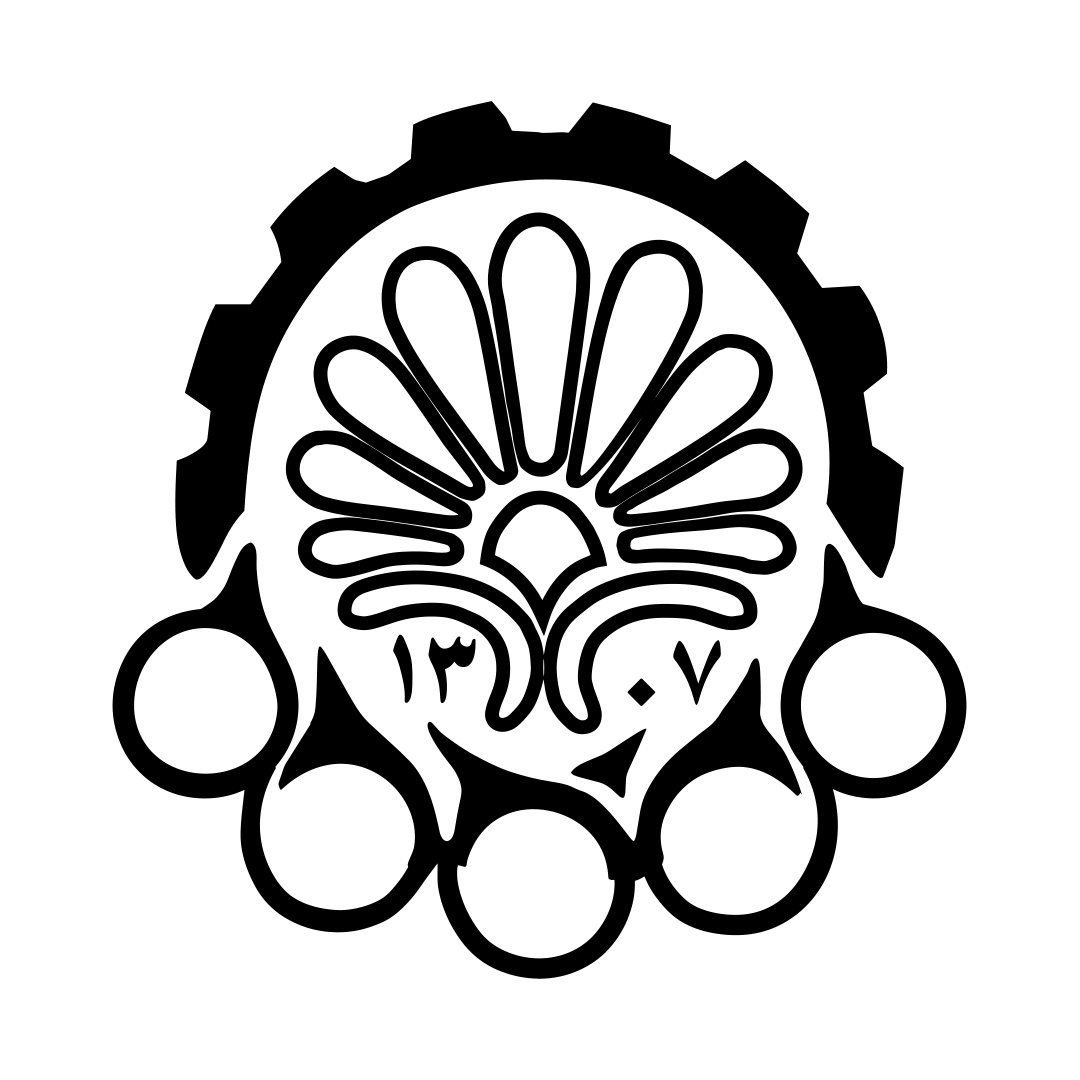
\includegraphics[width=44mm]{assets/aut-logo-black.png}\par
    \vspace{3mm}

    {\Large\bfseries \universityname\par}
    \vspace{1mm}
    {\large (\universityalias)\par}
    \vspace{1mm}
    {\large \facultyname\par}

    \vspace{8mm}
    {\Large\bfseries درس \coursename\par}

    \vspace{12mm}
    {\large عنوان\par}
    \vspace{2mm}
    {\LARGE\bfseries تمرین شماره \assignmentnumber\par}

    \vspace{10mm}
    {\large تهیه‌کننده\par}
    \vspace{2mm}
    {\Large\bfseries \studentname\par}

    \vspace{10mm}
    {\large استاد درس\par}
    \vspace{2mm}
    {\Large\bfseries \instructorname\par}

    \vspace{10mm}
    {\Large \assignmentdate\par}
    \vfill
  \end{titlepage}
  \setcounter{page}{1}%
}


\XeTeXgenerateactualtext=1
\newcommand{\secnum}[1]{\texorpdfstring{\mbox{\beginL#1\endL}}{#1}}
\newcommand{\code}[1]{\lr{\texttt{#1}}}
% Keep hierarchical counters in logical left-to-right order with localized digits.
\renewcommand{\thesection}{\texorpdfstring{\secnum{\arabic{chapter}.\arabic{section}}}{\arabic{chapter}.\arabic{section}}}
\renewcommand{\thesubsection}{\texorpdfstring{\secnum{\arabic{chapter}.\arabic{section}.\arabic{subsection}}}{\arabic{chapter}.\arabic{section}.\arabic{subsection}}}
\renewcommand{\thesubsubsection}{\texorpdfstring{\secnum{\arabic{chapter}.\arabic{section}.\arabic{subsection}.\arabic{subsubsection}}}{\arabic{chapter}.\arabic{section}.\arabic{subsection}.\arabic{subsubsection}}}
\counterwithin*{equation}{section}
\renewcommand{\theHequation}{\arabic{chapter}.\arabic{section}.\arabic{equation}}
\renewcommand{\theequation}{\texorpdfstring{\secnum{\theHequation}}{\theHequation}}
\renewcommand{\thefigure}{\texorpdfstring{\secnum{\arabic{chapter}.\arabic{figure}}}{\arabic{chapter}.\arabic{figure}}}
\renewcommand{\thetable}{\texorpdfstring{\secnum{\arabic{chapter}.\arabic{table}}}{\arabic{chapter}.\arabic{table}}}
\makeatletter
\renewcommand{\@pnumwidth}{2.5em}
\renewcommand{\@tocrmarg}{3.5em}
\makeatother
% Preserve the reviewed fragments while nesting their teaching units under the source section.
\newcommand{\BookletSubsections}[1]{%
  \begingroup
  \let\section\subsection
  \let\subsection\subsubsection
  \input{#1}%
  \endgroup
}
\setlength{\emergencystretch}{3em}
\widowpenalty=10000
\clubpenalty=10000
\setcounter{secnumdepth}{3}
\AtBeginDocument{\DeclareSIPrefix{\micro}{\text{\lr{µ}}}{-6}}
\patchcmd{\MakeAssignmentCover}{تمرین شماره \assignmentnumber}{\assignmentnumber}{}{\errmessage{Cover title replacement failed}}
% Shared bibliographic text. Coverage notes remain in each booklet.
\newcommand{\WesteReference}{%
\begin{latin}
Neil H. E. Weste and David Money Harris,
\textit{CMOS VLSI Design: A Circuits and Systems Perspective},
Fourth Edition, Addison-Wesley (Pearson Education), 2011.
\end{latin}%
}


% The complete edition continues textbook chapter 2 across all three booklets.
\newif\ifCompleteNotes
\newcommand{\NotesTopic}[2]{%
  \ifCompleteNotes\hyperref[#1]{#2}\else#2\fi
}
% Topic reviews are nested under their host section in the comprehensive notes.
\newcommand{\BookletReview}[1]{%
  \ifCompleteNotes
    \begingroup
    \let\chapter\subsection
    \let\section\subsubsection
    \let\BookletAddContentsLine\addcontentsline
    \renewcommand{\addcontentsline}[3]{%
      \ifstrequal{##2}{chapter}
        {\BookletAddContentsLine{##1}{subsection}{##3}}
        {\ifstrequal{##2}{section}
          {\BookletAddContentsLine{##1}{subsubsection}{##3}}
          {\BookletAddContentsLine{##1}{##2}{##3}}}%
    }%
    \input{#1}%
    \endgroup
  \else
    \input{#1}%
  \fi
}

\CompleteNotestrue
\setcounter{tocdepth}{3}
\makeatletter
\renewcommand{\@pnumwidth}{3em}
\renewcommand{\@tocrmarg}{4em}
\makeatother
% PDF bookmarks need literal Persian digits independently of font digit mapping.
\makeatletter
\newcommand{\PersianBookmarkCounter}[1]{%
  \expandafter\PersianBookmarkDigits\number\value{#1}\@nil
}
\def\PersianBookmarkDigits#1{%
  \ifx#1\@nil
  \else
    \ifcase#1۰\or۱\or۲\or۳\or۴\or۵\or۶\or۷\or۸\or۹\fi
    \expandafter\PersianBookmarkDigits
  \fi
}
\makeatother
\renewcommand{\thechapter}{\texorpdfstring{\arabic{chapter}}{\PersianBookmarkCounter{chapter}}}
\renewcommand{\thesection}{\texorpdfstring{\secnum{\arabic{chapter}.\arabic{section}}}{\PersianBookmarkCounter{chapter}.\PersianBookmarkCounter{section}}}
\renewcommand{\thesubsection}{\texorpdfstring{\secnum{\arabic{chapter}.\arabic{section}.\arabic{subsection}}}{\PersianBookmarkCounter{chapter}.\PersianBookmarkCounter{section}.\PersianBookmarkCounter{subsection}}}
\renewcommand{\thesubsubsection}{\texorpdfstring{\secnum{\arabic{chapter}.\arabic{section}.\arabic{subsection}.\arabic{subsubsection}}}{\PersianBookmarkCounter{chapter}.\PersianBookmarkCounter{section}.\PersianBookmarkCounter{subsection}.\PersianBookmarkCounter{subsubsection}}}
\hypersetup{pdftitle={جزوه جامع مبانی CMOS VLSI},pdfauthor={محمد خلیلی اصل},bookmarksnumbered=true}
\AssignmentNumber{جزوه جامع مبانی \lr{CMOS VLSI}}
\AssignmentDate{}
\begin{document}
\MakeAssignmentCover
% !TeX root = ../complete.tex
\chapter*{راهنمای مطالعه}
\phantomsection
\addcontentsline{toc}{chapter}{راهنمای مطالعه}

این جزوه از مبانی ریاضی، مدار و منطق دیجیتال آغاز می‌شود و به تحلیل
ترانزیستور \lr{MOS} و رفتار مدارهای \lr{CMOS} می‌رسد. آشنایی قبلی با
\lr{Digital Electronics} پیش‌نیاز مطالعه نیست. برای شروع، محاسبه با اعداد
و خواندن یک تساوی ساده کافی است. فصل صفر ابزارهای لازم را با مثال آموزش می‌دهد.

\subsection*{مسیر مطالعه}
در خواندن نخست، از \hyperref[chap:foundations]{فصل صفر} آغاز کنید. در
\hyperref[chap:introduction]{فصل ۱}، مسیر اتصال ترانزیستورها به گیت‌ها،
بلوک‌ها و طرح فیزیکی تراشه را دنبال کنید. در \hyperref[chap:mos-theory]{فصل ۲}،
ابتدا مدل جریان و ظرفیت را یاد بگیرید. سپس بررسی کنید اثرهای غیرایده‌آل
چه تغییری در مدل ایجاد می‌کنند و مدل جریان چگونه رفتار \lr{Inverter}
و \lr{Pass Transistor} را توضیح می‌دهد.

پیش از خواندن پاسخ هر مثال، شکل مدار را رسم کنید، مرجع ولتاژ و جهت
جریان را مشخص کنید و شرط‌های مدل را بنویسید. پس از حل، واحدها، علامت‌ها
و اعتبار ناحیه‌ی کاری را بررسی کنید. هنگام مرور، از جدول تطبیق منابع
به مبحث موردنیاز بروید و یکی از تمرین‌های همان مبحث را دوباره حل کنید.

\subsection*{دانش موردنیاز و محل یادگیری}
\begin{itemize}
  \item \hyperref[sec:foundation-math]{ریاضی فصل صفر} از کسر، نسبت، توان،
    نماد علمی و تبدیل واحد شروع می‌شود و به حل معادله، انتخاب ریشه‌ی
    فیزیکی و خواندن نمودار و شیب می‌رسد. این ابزارها در محاسبه‌ی جریان
    و ظرفیت و حل ولتاژ خروجی به کار می‌روند.
  \item آموزش \hyperref[sec:foundation-circuits]{مدار} و منطق در فصل صفر، ولتاژ مرجع،
    جهت جریان، تعادل گره، بار و ظرفیت، و معنای صفر و یک و گیت‌ها را
    معرفی می‌کند. این مفاهیم برای تحلیل مسیر هدایت و تعادل جریان
    خروجی لازم‌اند.
  \item تغییر ولتاژ در زمان و نقش مشتق در
    \hyperref[eq:foundation-rc-ode]{پاسخ مدار \lr{RC}} معرفی می‌شود.
    تابع نماییِ پاسخ را می‌توان با خواندن نمودار دنبال کرد.
    انتگرال به‌صورت جمع پیوسته در
    \hyperref[sec:book-mos-current]{استخراج جریان \lr{Long-channel}}
    معرفی می‌شود. \hyperref[sec:subthreshold-leakage]{تحلیل نشتی زیرآستانه}
    تابع نمایی، لگاریتم و خواندن محور لگاریتمی را مرور می‌کند.
    \hyperref[sec:noise-derivatives]{استخراج شیب در بحث \lr{Noise Margin}}
    مشتق‌گیری لازم برای یافتن نقاط شیب منفی یک را توضیح می‌دهد.
\end{itemize}

\clearpage
\subsection*{تطبیق موضوع‌ها با کتاب و اسلایدها}
جدول، مسیر دسترسی از بخش‌های کتاب \lr{Weste} و \lr{Harris} به
موضوع‌های متن و مجموعه‌اسلایدهای مرتبط را نشان می‌دهد \cite{weste}.
شماره‌های همراه با «کتاب» یا «اسلاید» به همان منبع تعلق دارند.
مثال‌های آموزشی با داده‌های فرضی، روش محاسبه را نشان می‌دهند.
پارامترهای فناوری را با فرض‌ها و زمینه‌ی همان مثال بخوانید.

\begin{center}
\small
\begin{tabularx}{\textwidth}{rXr}
\toprule
بخش کتاب & موضوع در جزوه & اسلاید مرتبط\\
\midrule
\secnum{۱.۱} تا \secnum{۱.۳} & \hyperref[sec:ch1-history]{تاریخچه}، مسیر طراحی و ساختار \lr{MOS} & \cite{intro,mos}\\
\secnum{۱.۴} & \hyperref[sec:book-cmos]{گیت، انتخاب و ذخیره‌ی داده} & \cite{intro}\\
\secnum{۱.۵} & \hyperref[sec:book-fabrication]{ساخت و \lr{Layout}} & \cite{mos}\\
\secnum{۱.۶} & \hyperref[sec:book-partitioning]{سطوح و دامنه‌های طراحی} & \cite{intro}\\
\secnum{۱.۷} و \secnum{۱.۸} & \hyperref[sec:book-mips]{مثال \lr{MIPS}} و \hyperref[sec:book-logic-design]{طراحی منطقی و \lr{HDL}} & \cite{intro}\\
\secnum{۱.۹} تا \secnum{۱.۱۲} & طراحی مدار و طرح فیزیکی، بررسی و \hyperref[sec:book-manufacturing]{تولید} & تکمیل از کتاب\\
\secnum{۲.۱} & \hyperref[sec:book-mos-structure]{ساختار ترانزیستور و تشکیل کانال} & \cite[اسلایدهای ۲ تا ۱۳]{mos}\\
\secnum{۲.۲} & \hyperref[sec:book-mos-current]{مدل جریان \lr{Long-channel}} & \cite[اسلایدهای ۱۴ تا ۲۲]{mos}\\
\secnum{۲.۳} & \hyperref[sec:book-cv]{ظرفیت و هندسه‌ی ترانزیستور} & \cite[اسلایدهای ۲۳ و ۲۴]{mos}\\
\secnum{۲.۴} & \hyperref[sec:nonideal-current]{اثر میدان، تغییر طول کانال، آستانه و نشتی} & \cite[اسلایدهای ۳ تا ۳۷]{nonideal}\\
\secnum{۲.۵} & \hyperref[sec:dc-transfer]{مشخصه‌ی انتقال \lr{DC}}، \hyperref[sec:noise-margin]{حاشیه‌ی نویز} و \hyperref[sec:pass-transistor]{انتقال ولتاژ} & \cite[اسلایدهای ۳ تا ۱۴]{dcslides}\\
\bottomrule
\end{tabularx}
\end{center}

\tableofcontents
% !TeX root = booklet-01.tex
\clearpage
\setcounter{chapter}{-1}
\chapter{پیش‌نیازهای ریاضی، مدار و منطق دیجیتال}
\label{chap:foundations}
این فصل، پایه لازم برای خواندن درس بدون گذراندن \lr{Digital Electronics} را
فراهم می‌کند. ابتدا محاسبه و واحد، سپس قوانین مدار و در پایان منطق دیجیتال
آموزش داده می‌شود. مثال‌ها و پاسخ‌ها را به ترتیب دنبال کنید.
% !TeX root = booklet-01.tex
\section{زبان ریاضی لازم برای خواندن مدار}
\label{sec:foundation-math}
فرمول یک رابطه میان کمیت‌هاست. پیش از محاسبه باید بدانیم هر حرف چه کمیتی را
نمایش می‌دهد، واحد آن چیست و رابطه تحت چه فرضی به کار می‌رود.
در این درس، حفظ شکل رابطه بدون شناخت این سه مورد می‌تواند به جواب عددی ظاهراً درست
اما از نظر فیزیکی نامعتبر منجر شود.

\subsection{نماد، زیرنویس، کسر و نسبت}
حرفی مانند \(V\) می‌تواند نماد ولتاژ باشد؛ زیرنویس آن مشخص می‌کند کدام ولتاژ
منظور است. برای مثال، \(V_a\) ولتاژ گره \(a\) و \(V_{ab}\) اختلاف ولتاژ
گره \(a\) نسبت به \(b\) است. زیرنویس، ضرب نیست: \(V_a\) به معنی \(V\times a\) نیست.
نماد \(\Delta\) نیز تغییر کمیت را نشان می‌دهد. برای نمونه، تغییر ولتاژ را
به صورت زیر تعریف می‌کنیم.
\[
 \Delta V=V_{\mathrm{final}}-V_{\mathrm{initial}}.
\]
واژه‌های زیرنویس \(\mathrm{final}\) و \(\mathrm{initial}\) به‌ترتیب حالت نهایی و اولیه‌اند.

در کسر \(a/b\)، صورت \(a\) بر مخرج \(b\) تقسیم می‌شود و باید \(b\ne0\) باشد.
نسبت دو کمیت هم‌واحد، بدون واحد است. مثلاً نسبت \(\qty{6}{\volt}\)
به \(\qty{2}{\volt}\) برابر ۳ است؛ ولی نسبت ولتاژ به جریان واحد دارد
و می‌تواند مقاومت را بیان کند. پس واحدها بخشی از استدلال‌اند.

برای دیدن اثر یک پارامتر، نخست سایر پارامترها را ثابت می‌گیریم.
در رابطه \(y=kx\)، اگر \(k\) ثابت باشد، دو برابر شدن \(x\)، مقدار \(y\) را
دو برابر می‌کند. در \(y=k/x\)، با \(k\) ثابت و \(x\ne0\)، دو برابر شدن
\(x\)، مقدار \(y\) را نصف می‌کند. این نتیجه‌ها وقتی سایر پارامترها نیز
تغییر کنند الزاماً برقرار نیستند.

\subsection{توان و نماد علمی}
توان مثبت، ضرب تکراری است. برای پایه ده و توان سه داریم
\[
 10^3=10\times10\times10=1000.
\]
توان منفی یعنی معکوس توان مثبت. برای همان پایه و توان منفی سه داریم
\[
 10^{-3}=\frac{1}{10^3}=0.001.
\]
قواعد زیر برای پایه مثبت \(a\) و توان‌های مورد استفاده در این جزوه به کار می‌روند:
\begin{equation}\label{eq:foundation-powers}
a^m a^n=a^{m+n},\qquad
\frac{a^m}{a^n}=a^{m-n},\qquad
(a^m)^n=a^{mn}.
\end{equation}
برای نمونه، قانون تفریق توان‌ها در تقسیم می‌دهد
\[
 \frac{10^{-12}}{10^{-9}}=10^{-12-(-9)}=10^{-3}.
\]
دو علامت منفی در تفریق توان‌ها حذف می‌شوند؛ نتیجه \(10^{-21}\) نیست.

در نماد علمی، عدد را به صورت \(b\times10^n\) می‌نویسیم؛ برای عدد مثبت،
معمولاً \(1\le b<10\) است. مثلاً \(0.000024=2.4\times10^{-5}\).
در جمع، باید ابتدا توان‌ها یکسان شوند:
\[
2\times10^{-3}+3\times10^{-4}
=20\times10^{-4}+3\times10^{-4}
=23\times10^{-4}=2.3\times10^{-3}.
\]
قانون جمع توان‌ها در رابطه \eqref{eq:foundation-powers} برای ضرب است؛
به جمع دو عدد تعمیم داده نمی‌شود.

\subsection{واحد و تبدیل پیشوند}
واحدهای مورد استفاده را در جدول \ref{tab:foundation-units} می‌بینیم.
نماد واحد با نماد متغیر تفاوت دارد؛ مثلاً \(C\) متغیر ظرفیت،
ولی \(\mathrm{C}\) نماد واحد بار است.
\begin{table}[ht]
\centering
\caption{کمیت‌ها و واحدهای اصلی این بخش}
\label{tab:foundation-units}
\begin{tabular}{ccc}
\toprule
کمیت & نماد متداول & واحد \lr{SI}\\
\midrule
بار & \(Q\) & \(\mathrm{C}\)\\
جریان & \(I\) & \(\mathrm{A}\)\\
ولتاژ & \(V\) & \(\mathrm{V}\)\\
مقاومت & \(R\) & \(\Omega\)\\
ظرفیت & \(C\) & \(\mathrm{F}\)\\
زمان & \(t\) & \(\mathrm{s}\)\\
انرژی & \(E\) & \(\mathrm{J}\)\\
توان & \(P\) & \(\mathrm{W}\)\\
\bottomrule
\end{tabular}
\end{table}

پیشوندهای \lr{kilo}، \lr{milli}، \lr{micro}، \lr{nano}، \lr{pico} و
\lr{femto} به‌ترتیب ضرایب \(10^3\)، \(10^{-3}\)، \(10^{-6}\)،
\(10^{-9}\)، \(10^{-12}\) و \(10^{-15}\) هستند.
پس \(\qty{2}{\kilo\ohm}=\qty{2000}{\ohm}\) و
\(\qty{20}{\femto\farad}=20\times10^{-15}\,\mathrm{F}\).

\textbf{مثال آموزشی.} برای محاسبه زمان از نسبت بار به جریان، فرض کنید
\(Q=\qty{6}{\pico\coulomb}\) و جریان ثابت \(I=\qty{3}{\milli\ampere}\) باشد:
\begin{align*}
t&=\frac{Q}{I}
=\frac{6\times10^{-12}\,\mathrm{C}}{3\times10^{-3}\,\mathrm{A}}\\
&=2\times10^{-9}\,\mathrm{s}=\qty{2}{\nano\second}.
\end{align*}
چون \(\mathrm{A}=\mathrm{C}/\mathrm{s}\)، واحد کسر برابر ثانیه می‌شود.
این کنترل واحد، مستقل از حساب عددی است و خطای استفاده از \(I/Q\) را آشکار می‌کند.

\subsection{حل معادله با حفظ تساوی}
معادله یعنی دو عبارت مقدار یکسان دارند. برای حفظ این برابری، باید عملی یکسان
روی هر دو طرف انجام دهیم. در \(V=RI\)، برای پیدا کردن جریان و با فرض \(R\ne0\)،
دو طرف را بر \(R\) تقسیم می‌کنیم تا \(I=V/R\) به دست آید.

\textbf{مثال آموزشی.} معادله \(3x+2=11\) را حل کنیم. ابتدا از دو طرف ۲ کم
می‌کنیم و سپس دو طرف را بر ۳ تقسیم می‌کنیم.
\[
 \begin{aligned}
 3x&=9,\\
 x&=3.
 \end{aligned}
\]
جای‌گذاری در معادله اولیه می‌دهد \(3\times3+2=11\).
منظور از «انتقال جمله به طرف دیگر»، همین عمل روی دو طرف است؛ علامت‌ها بی‌دلیل تغییر نمی‌کنند.

توزیع ضرب روی پرانتز یعنی \(a(b+c)=ab+ac\).
بنابراین \(2(x-3)=2x-6\)، نه \(2x-3\).
همچنین \((x-y)^2=x^2-2xy+y^2\)؛ جمله میانی را نباید حذف کرد.
برای تقسیم بر یک عبارت حاوی مجهول، باید صفر نبودن آن را بررسی کنیم؛
تقسیم معادله \(x(x-1)=0\) بر \(x\)، جواب مجاز \(x=0\) را از دست می‌دهد.

\subsection{معادله درجه‌دو و انتخاب ریشه فیزیکی}
وقتی جمله \(x^2\) داریم، ممکن است دو جواب ریاضی وجود داشته باشد.
برای \(ax^2+bx+c=0\) با \(a\ne0\)، تعریف \(D=b^2-4ac\) می‌دهد:
\begin{equation}\label{eq:foundation-quadratic}
x=\frac{-b\pm\sqrt{D}}{2a}.
\end{equation}
در اعداد حقیقی، اگر \(D<0\) باشد جواب حقیقی نداریم؛ اگر \(D=0\)،
دو ریشه بر هم منطبق‌اند و اگر \(D>0\)، دو ریشه متمایز داریم.
نماد \(\pm\) یعنی یک‌بار علامت مثبت و یک‌بار منفی را به کار ببریم.

\textbf{مثال آموزشی بدون واحد.} فرض کنید \(x^2-3x+2=0\) و مسئله شرط
\(0\le x\le1.5\) را نیز داده باشد. در اینجا \(a=1\)، \(b=-3\) و \(c=2\) است:
\[
D=(-3)^2-4(1)(2)=1,\qquad
x=\frac{3\pm1}{2}.
\]
ریشه‌ها ۱ و ۲ هستند. هر دو معادله را ارضا می‌کنند؛ فقط ریشه ۱ در بازه مجاز است.
پس جواب مسئله ۱ است، نه صرفاً ریشه مثبت؛ هر دو ریشه در این مثال مثبت‌اند.
در تحلیل ترانزیستور نیز علاوه بر معادله، باید شرط ناحیه عملکرد و بازه ولتاژها برقرار باشد.

\subsection{خواندن نمودار و معنای شیب}
در نمودار \(y=f(x)\)، محور افقی مقدار \(x\) و محور عمودی مقدار متناظر \(y\)
را نشان می‌دهد. عبارت \(f(x)\) نام یک قانون وابستگی است؛ ضرب \(f\) در \(x\) نیست.
برای دو نقطه، شیب متوسط را تعریف می‌کنیم:
\begin{equation}\label{eq:foundation-slope}
m=\frac{y_2-y_1}{x_2-x_1},\qquad x_2\ne x_1.
\end{equation}
شیب مثبت یعنی در این بازه با افزایش \(x\)، مقدار \(y\) افزایش یافته است؛
شیب منفی یعنی کاهش یافته است. واحد شیب، واحد محور عمودی تقسیم بر واحد محور افقی است.
مثلاً اگر ولتاژ در \(\qty{2}{\nano\second}\) از صفر به \(\qty{1}{\volt}\) برسد،
شیب متوسط \(\qty{0.5}{\volt\per\nano\second}\) است.

مشتق، حد همین نسبت در یک بازه بسیار کوچک است؛ نوشتن \(\mathrm{d}V/\mathrm{d}t\)
یعنی شیب لحظه‌ای نمودار ولتاژ نسبت به زمان، نه تقسیم خود \(V\) بر خود \(t\).
برای خط راست، شیب در همه نقاط ثابت و با شیب متوسط برابر است؛ برای منحنی چنین نیست.
آموزش استخراج مشتق‌ها در محل استفاده از آن‌ها ادامه خواهد یافت.

\subsection{سنجش فهم ریاضی}
\begin{enumerate}
\item \textbf{آیا \(10^{-6}+10^{-6}=10^{-12}\) است؟}
خیر؛ مجموع \(2\times10^{-6}\) است. حاصل‌ضرب آن دو برابر \(10^{-12}\) می‌شود.
\item \textbf{در \(I=V/R\)، با ثابت بودن \(V\)، سه برابر شدن مقاومت چه اثری دارد؟}
جریان به یک‌سوم می‌رسد؛ زیرا مخرج سه برابر شده است.
\item \textbf{آیا هر ریشه‌ای که معادله را ارضا کند جواب مدار است؟}
خیر؛ باید با واحدها، بازه مجاز، اتصال‌ها و فرض‌های مدل نیز سازگار باشد.
\end{enumerate}

% !TeX root = booklet-01.tex
\section{کمیت‌های الکتریکی و خواندن اتصال‌ها}
\label{sec:foundation-circuits}
\subsection{بار، جریان و جهت مرجع}
بار الکتریکی با \(Q\) و واحد \lr{coulomb} نمایش داده می‌شود.
جریان متوسط، بار خالص عبوری از یک مقطع در واحد زمان است \cite{current}:
\begin{equation}\label{eq:foundation-current}
I_{\mathrm{avg}}=\frac{\Delta Q}{\Delta t}.
\end{equation}
برای مثال، عبور \(\qty{6}{\pico\coulomb}\) در \(\qty{2}{\nano\second}\)،
جریان متوسط \(\qty{3}{\milli\ampere}\) می‌دهد.
این رابطه از شکل تغییر جریان در طول بازه اطلاعی نمی‌دهد.
جریان لحظه‌ای با \(i(t)=\mathrm{d}Q/\mathrm{d}t\) بیان می‌شود؛ معنای نرخ تغییر
در بخش \ref{sec:foundation-math} توضیح داده شد.

جهت جریان قراردادی، جهت حرکت بار مثبت است؛ برای حرکت \lr{Electron} در فلز،
جهت حرکت حامل و جریان مخالف‌اند \cite{current}.
در تحلیل، ابتدا یک پیکان مرجع انتخاب می‌کنیم. اگر پاسخ جریان منفی شد،
جهت واقعی مخالف پیکان است؛ منفی شدن لزوماً نشانه اشتباه محاسبه نیست.

\subsection{ولتاژ، مرجع و تفاوت انرژی و توان}
ولتاژ، اختلاف پتانسیل است. تغییر انرژی پتانسیل بار مثبت \(q\) در جابه‌جایی
از نقطه \(b\) به \(a\)، برابر \(\Delta U=q(V_a-V_b)\) است.
بنابراین واحد ولتاژ، انرژی بر بار است:
\(\qty{1}{\volt}=\qty{1}{\joule\per\coulomb}\).
ولتاژ دو نقطه را با ترتیب مشخص تعریف می‌کنیم:
\begin{equation}\label{eq:foundation-voltage}
V_{ab}=V_a-V_b,\qquad V_{ba}=-V_{ab}.
\end{equation}
اگر \(V_a=\qty{1}{\volt}\) و \(V_b=\qty{0.4}{\volt}\)،
داریم \(V_{ab}=\qty{0.6}{\volt}\).
ولتاژ گره به‌تنهایی، همیشه نسبت به مرجعی مثل \lr{Ground} معنا دارد.
تغییر مرجع مشترک، اختلاف ولتاژ واقعی دو گره را تغییر نمی‌دهد.

انرژی مقدار کار قابل مبادله است؛ توان، نرخ مبادله انرژی است.
اگر جریان \(i\) وارد سر مثبت ولتاژ \(v\) یک جزء شود، توان جذب‌شده آن جزء
\(p=vi\) است. حاصل مثبت یعنی جذب و حاصل منفی یعنی تحویل انرژی به مدار.
این رابطه و کاربرد \(P=VI\) در تحلیل توان مدار با بخش \secnum{۱.۹} کتاب مرتبط‌اند
\cite{weste}. مثلاً یک مقاومت با ولتاژ \(\qty{1}{\volt}\) و جریان
\(\qty{1}{\milli\ampere}\)، توان \(\qty{1}{\milli\watt}\) جذب می‌کند؛
اگر این وضع \(\qty{2}{\milli\second}\) ثابت بماند، انرژی جذب‌شده
\(E=Pt=\qty{2}{\micro\joule}\) است. انرژی و توان هم‌واحد نیستند.

\subsection{گره، شاخه، مدار باز و اتصال کوتاه}
\lr{Node} مجموعه نقاطی است که با سیم ایدئال مستقیم متصل و هم‌پتانسیل‌اند.
وجود یک قطعه میان دو نقطه، معمولاً آن‌ها را به دو گره متفاوت تبدیل می‌کند.
\lr{Branch} یک مسیر میان دو گره است که جریان آن را در تحلیل مشخص می‌کنیم.
\lr{Ground} گره مرجع با ولتاژ صفر است؛ الزامی ندارد به زمین فیزیکی متصل باشد.

در نقشه‌های کتاب، اتصال به‌شکل \lr{T} متصل است؛ برای تقاطع دو سیم،
وجود نقطه، اتصال را مشخص می‌کند \cite[بخش \secnum{۱.۴.۲}]{weste}.
ظاهر نزدیک یا دور دو قطعه معیار هم‌گره بودن نیست؛ مسیر سیم را باید دنبال کرد.

در مدل \lr{Open Circuit}، جریان مسیر باز صفر است، ولی اختلاف ولتاژ دو سر آن
می‌تواند غیرصفر باشد. در مدل \lr{Short Circuit}، اختلاف ولتاژ صفر است؛
جریان را بقیه مدار تعیین می‌کند. اتصال کوتاه مستقیم دو سر منبع ولتاژ ایدئال
غیرصفر، مدلی ناسازگار ایجاد می‌کند؛ برای محاسبه جریان واقعی باید مقاومت‌ها و
محدودیت‌های منبع را در نظر گرفت.

\section{قوانین مدار و روش تحلیل}
\subsection{مقاومت و \lr{Ohm's Law}}
برای مقاومت خطی مثبت \(R\)، با ورود جریان مرجع به سر مثبت ولتاژ، داریم
\cite{resistors}:
\begin{equation}\label{eq:foundation-ohm}
v=Ri,\qquad i=\frac{v}{R}.
\end{equation}
مقاومت بزرگ‌تر در ولتاژ ثابت، جریان کمتری می‌دهد.
اگر جریان محاسبه‌شده منفی شود، جهت مرجع برعکس جریان واقعی بوده است.
از \(p=vi\) و رابطه \eqref{eq:foundation-ohm} نتیجه می‌گیریم
\(p=Ri^2=v^2/R\ge0\). پس مقاومت مثبت در این مدل انرژی تولید نمی‌کند.
ترانزیستور را نباید در تمام ناحیه‌های عملکرد، یک مقاومت ثابت فرض کرد؛
رابطه جریان آن در ادامه جزوه استخراج خواهد شد.

\subsection{قانون گره: \lr{KCL}}
در مدل مدار متمرکز، با حساب‌کردن جریان تمام شاخه‌ها از جمله شاخه‌های خازنی،
مجموع جریان‌های ورودی به گره با مجموع جریان‌های خروجی برابر است
\cite{kirchhoff}. این قانون با نام \lr{Kirchhoff's Current Law (KCL)} شناخته می‌شود:
\begin{equation}\label{eq:foundation-kcl}
\sum I_{\mathrm{in}}=\sum I_{\mathrm{out}}.
\end{equation}
نماد \(\sum\) یعنی جمع‌کردن همه جمله‌های مربوط.
مثلاً اگر \(\qty{3}{\milli\ampere}\) وارد گره و
\(\qty{1}{\milli\ampere}\) از یک شاخه خارج شود، جریان خروجی شاخه دیگر
\(\qty{2}{\milli\ampere}\) است. اگر خروجی به خازن متصل باشد، نباید
جریان شارژ آن را از معادله حذف کنیم.

\subsection{قانون حلقه: \lr{KVL}}
در تحلیل مدار متمرکز و با صرف‌نظر از القای مغناطیسی مدل‌نشده، جمع جبری تغییرات
ولتاژ در پیمودن یک مسیر بسته صفر است \cite{kirchhoff}.
این \lr{Kirchhoff's Voltage Law (KVL)} است:
\begin{equation}\label{eq:foundation-kvl}
\sum_{\mathrm{loop}}\Delta V=0.
\end{equation}
در عبور از منبع از پایانه منفی به مثبت، افزایش ولتاژ داریم؛ در عبور از مقاومت
در جهت جریان، افت \(IR\) داریم. مثلاً منبع \(V_s\) و دو مقاومت سری می‌دهند
\(V_s-IR_1-IR_2=0\). از اینجا
\(I=V_s/(R_1+R_2)\) به دست می‌آید. جهت پیمودن حلقه دلخواه است؛
باید علامت‌ها با همان انتخاب سازگار بمانند.

\subsection{اتصال \lr{Series} و \lr{Parallel} را از گره‌ها بشناسیم}
دو مقاومت وقتی سری‌اند که گره مشترکشان شاخه دیگری نداشته باشد؛ جریان یکسانی از
هر دو می‌گذرد. از جمع افت ولتاژها، \(R_{\mathrm{eq}}=R_1+R_2\) نتیجه می‌شود.
وقتی دو مقاومت دقیقاً میان دو گره یکسان باشند، موازی‌اند و ولتاژ یکسانی دارند.
با جمع جریان‌ها طبق \lr{KCL} به دست می‌آید \cite{resistors}:
\begin{align}
I&=\frac{V}{R_1}+\frac{V}{R_2}
=V\left(\frac{1}{R_1}+\frac{1}{R_2}\right),\notag\\
\frac{1}{R_{\mathrm{eq}}}&=\frac{1}{R_1}+\frac{1}{R_2},
\qquad R_{\mathrm{eq}}=\frac{R_1R_2}{R_1+R_2}.
\label{eq:foundation-parallel}
\end{align}
برای دو مقاومت مثبت، مقاومت معادل موازی از هر دو کمتر است؛ این یک کنترل مفید برای جواب است.
مثلاً دو مقاومت \(\qty{2}{\kilo\ohm}\) و \(\qty{3}{\kilo\ohm}\)،
در سری \(\qty{5}{\kilo\ohm}\) و در موازی \(\qty{1.2}{\kilo\ohm}\) می‌دهند.

\subsection{مثال کامل: استخراج ولتاژ یک گره}
در شکل \ref{fig:foundation-divider}، منبع ایدئال \(V_s\) و دو مقاومت مثبت داریم.
خروجی بار رسانشی ندارد. شکل برای همین جزوه رسم شده است.
\begin{figure}[ht]
\centering
\begin{latin}
\begin{circuitikz}[american]
\draw (0,0) node[ground] {} to[V,invert,l=$V_s$] (0,3)
 to[R,l=$R_1$] (3,3) to[R,l=$R_2$] (3,0) -- (0,0);
\draw (3,3) to[short,*-o] (4.7,3) node[right] {$V_x$};
\end{circuitikz}
\end{latin}
\caption{مدار آموزشی تقسیم ولتاژ؛ خروجی از گره مشترک دو مقاومت گرفته می‌شود.}
\label{fig:foundation-divider}
\end{figure}
جریان \(R_1\) را از منبع به گره \(x\) و جریان \(R_2\) را از گره به زمین
انتخاب می‌کنیم. ولتاژهای دو سر مقاومت‌ها به‌ترتیب \(V_s-V_x\) و \(V_x-0\) هستند.
با استفاده از \lr{Ohm's Law} و سپس \lr{KCL}:
\begin{align}
\frac{V_s-V_x}{R_1}&=\frac{V_x}{R_2},\notag\\
R_2(V_s-V_x)&=R_1V_x,\notag\\
R_2V_s&=(R_1+R_2)V_x,\notag\\
V_x&=V_s\frac{R_2}{R_1+R_2}.
\label{eq:foundation-divider}
\end{align}
در سطر دوم دو طرف را در \(R_1R_2\) ضرب کردیم؛ سپس پرانتز را باز و جمله‌های
حاوی \(V_x\) را یک طرف جمع کردیم. با \(V_s=\qty{1}{\volt}\)،
\(R_1=\qty{2}{\kilo\ohm}\) و \(R_2=\qty{3}{\kilo\ohm}\)،
داریم \(V_x=\qty{0.6}{\volt}\).
جریان هر دو مقاومت \(\qty{0.2}{\milli\ampere}\) و افت‌ها
\(\qty{0.4}{\volt}\) و \(\qty{0.6}{\volt}\) هستند؛ جمع افت‌ها با منبع برابر است.

\textbf{کنترل حدی و فرض بار.} با میل \(R_2\) به صفر، خروجی به صفر و با
بسیار بزرگ شدن آن نسبت به \(R_1\)، خروجی به \(V_s\) نزدیک می‌شود.
اگر بار مقاومتی \(R_L\) از خروجی به زمین وصل شود، در رابطه
\eqref{eq:foundation-divider} باید \(R_2\) را با \(R_2\parallel R_L\) جایگزین کرد؛
زیرا دیگر جریان \(R_1\) فقط از \(R_2\) نمی‌گذرد. نماد \(\parallel\) اتصال موازی را نشان می‌دهد.

\section{خازن، شارژ و مفهوم زمان}
\label{sec:foundation-capacitor}
\subsection{خازن چه چیزی را ذخیره می‌کند؟}
خازن از دو رسانا با ماده عایق میان آن‌ها ساخته می‌شود.
در مدل دوصفحه‌ای ایدئال، بارهای صفحات \(+Q\) و \(-Q\) هستند؛
مجموع بار دو صفحه می‌تواند صفر باشد، درحالی‌که انرژی در میدان ذخیره شده است
\cite{capacitors}. پس عبارت «بار خازن» معمولاً به بار علامت‌دار یک صفحه
یا اندازه بار صفحات اشاره دارد، نه مجموع آن دو.

اگر ظرفیت ثابت \(C\) باشد و \(v\) را ولتاژ صفحه اول نسبت به دوم بگیریم،
بار صفحه اول برابر است با:
\begin{equation}\label{eq:foundation-qcv}
Q=Cv,\qquad C=\frac{Q}{v}\quad(v\ne0).
\end{equation}
واحد ظرفیت \lr{farad} است و \(\mathrm{F}=\mathrm{C}/\mathrm{V}\).
مثلاً در خازن \(\qty{20}{\femto\farad}\)، ولتاژ \(\qty{1}{\volt}\)
با بار \(\qty{20}{\femto\coulomb}\) روی صفحه مثبت همراه است.
ظرفیت بزرگ‌تر در ولتاژ یکسان، بار بیشتری لازم دارد.

\subsection{از تغییر بار به تغییر ولتاژ}
برای ظرفیت ثابت، از رابطه \eqref{eq:foundation-qcv} داریم
\(\Delta Q=C\Delta v\). تقسیم دو طرف بر \(\Delta t\) و استفاده از تعریف
جریان متوسط می‌دهد:
\begin{equation}\label{eq:foundation-cap-current}
I_{\mathrm{avg}}=C\frac{\Delta v}{\Delta t},
\qquad i(t)=C\frac{\mathrm{d}v}{\mathrm{d}t}.
\end{equation}
در این قرارداد، جریان وارد صفحه‌ای می‌شود که ولتاژ مثبت برای آن تعریف شده است.
جریان مثبت بار آن صفحه و ولتاژ آن را افزایش می‌دهد؛ جریان منفی کاهش می‌دهد.
رابطه دوم شکل لحظه‌ای همان رابطه اول است. این ارتباط مبنای توضیح زمان تغییر خروجی
در کتاب و اسلاید است \cite[بخش \secnum{۱.۹}]{weste}\cite[اسلاید ۸]{mos}.
برای ظرفیت وابسته به ولتاژ، باید به رابطه عمومی \(i=\mathrm{d}Q/\mathrm{d}t\)
برگردیم؛ ثابت گرفتن \(C\) یک فرض مدل است.

\textbf{مثال آموزشی.} فرض کنیم جریان خالص ثابت \(I=\qty{10}{\micro\ampere}\)
به خازن \(C=\qty{20}{\femto\farad}\) وارد شود و ولتاژ آن از
\(\qty{0.2}{\volt}\) به \(\qty{0.8}{\volt}\) برسد. تغییر ولتاژ
\(\Delta v=\qty{0.6}{\volt}\) است. پس:
\begin{align}
\Delta t&=\frac{C\Delta v}{I}
=\frac{(20\times10^{-15}\,\mathrm{F})(0.6\,\mathrm{V})}
{10\times10^{-6}\,\mathrm{A}}\notag\\
&=1.2\times10^{-9}\,\mathrm{s}=\qty{1.2}{\nano\second}.
\label{eq:foundation-charge-time}
\end{align}
واحد \(\mathrm{F}\,\mathrm{V}/\mathrm{A}\) برابر ثانیه است.
در این مدل، دو برابر شدن ظرفیت، زمان را دو برابر و دو برابر شدن جریان، زمان را نصف می‌کند.
این نتیجه برای جریان ثابت است؛ جریان ترانزیستور واقعی عموماً طی تغییر ولتاژ ثابت نیست.

\subsection{حالت ماندگار، گذرا و پاسخ ساده \lr{RC}}
در حالت ماندگار \lr{DC}، ولتاژ خازن ثابت است؛ بنابراین در مدل ایدئال
\(\mathrm{d}v/\mathrm{d}t=0\) و جریان آن صفر می‌شود. این به معنی صفر بودن ولتاژ آن نیست.
در حالت گذرا، بار و ولتاژ تغییر می‌کنند. اختلاف ولتاژ خازن در حضور جریان محدود
نمی‌تواند ناگهان جهش کند؛ چون جهش نیازمند انتقال بار محدود در زمان صفر است.

برای درک تفاوت با جریان ثابت، خازنی را در نظر بگیرید که از منبع ثابت \(V_s\)
از طریق مقاومت \(R\) شارژ می‌شود؛ بار دیگری وجود ندارد و \(v(0)=0\).
با افزایش ولتاژ خازن، اختلاف ولتاژ مقاومت کم می‌شود؛ در نتیجه جریان
\(i=(V_s-v)/R\) کاهش می‌یابد. پس نمودار ولتاژ خط راست نیست.
از \lr{KCL} و رابطه \eqref{eq:foundation-cap-current} به دست می‌آید:
\begin{equation}\label{eq:foundation-rc-ode}
C\frac{\mathrm{d}v}{\mathrm{d}t}=\frac{V_s-v}{R}.
\end{equation}
جواب زیر فعلاً برای تفسیر معرفی می‌شود؛ می‌توان درستی آن را با مشتق‌گیری کنترل کرد:
\begin{equation}\label{eq:foundation-rc}
v(t)=V_s\left(1-e^{-t/(RC)}\right),\qquad t\ge0.
\end{equation}
عدد \(e\approx2.718\) پایه تابع نمایی است. برای عدد بی‌بعد مثبت \(x\)،
\(e^{-x}=1/e^x\)؛ با بزرگ شدن \(x\)، این مقدار به صفر نزدیک می‌شود.
حاصل \(RC\) واحد زمان دارد و آن را ثابت زمانی \(\tau=RC\) می‌نامیم.
در \(t=0\)، جواب صفر است؛ در \(t=\tau\)، مقدار ولتاژ تقریباً
\(0.632V_s\) و با زیاد شدن زمان، حد آن \(V_s\) است.
در مدل ایدئال نمایی، رسیدن دقیق به حد در زمان محدود رخ نمی‌دهد.

شکل \ref{fig:foundation-rc} همین پاسخ را بدون وابستگی به مقیاس یک فناوری
نشان می‌دهد. محور افقی زمان تقسیم بر ثابت زمانی و محور عمودی ولتاژ تقسیم بر
ولتاژ منبع است؛ هر دو نسبت بدون واحدند. کم‌شدن شیب یعنی کاهش جریان شارژ.
\begin{figure}[ht]
\centering
\begin{latin}
\begin{tikzpicture}[x=1.6cm,y=2.6cm]
\draw[->] (0,0) -- (3.6,0) node[right] {$t/\tau$};
\draw[->] (0,0) -- (0,1.25) node[above] {$v/V_s$};
\draw[dashed] (0,1) -- (3.3,1);
\node[left] at (0,1) {\rl{۱}};
\node[below left] at (0,0) {\rl{۰}};
\foreach \x/\ticklabel in {1/۱,2/۲,3/۳} {\draw (\x,0.025) -- (\x,-0.025) node[below] {\rl{\ticklabel}};}
\draw[thick,domain=0:3.3,samples=70] plot (\x,{1-exp(-\x)});
\draw[dotted] (1,0) -- (1,{1-exp(-1)}) -- (0,{1-exp(-1)});
\fill (1,{1-exp(-1)}) circle (1.4pt);
% Match the shared digit font for the Persian decimal separator.
\node[left] at (0,{1-exp(-1)}) {\fontspec[Path=C:/Windows/Fonts/]{arial.ttf}\mbox{\beginL۰٫۶۳۲\endL}};
\end{tikzpicture}
\end{latin}
\caption{نمودار تحلیلی پاسخ \lr{RC} رابطه \eqref{eq:foundation-rc}؛
این شکل از خود رابطه رسم شده است و نتیجه شبیه‌سازی \lr{SPICE} نیست.}
\label{fig:foundation-rc}
\end{figure}

برای دیدن سازگاری جواب با معادله، پاسخ و مشتق آن را کنار هم می‌نویسیم.
\[
 \begin{aligned}
 v&=V_s(1-e^{-t/\tau}),\\
 \frac{\mathrm{d}v}{\mathrm{d}t}&=\frac{V_s}{\tau}e^{-t/\tau}.
 \end{aligned}
\]
پس دو طرف رابطه \eqref{eq:foundation-rc-ode} برابر
\((V_s/R)e^{-t/\tau}\) می‌شوند. قاعده مشتق نمایی در اینجا معرفی شده است؛
استخراج تفصیلی قواعد مشتق در محل نیاز بعدی آموزش داده می‌شود.

\subsection{پرسش‌های مدار با پاسخ}
\begin{enumerate}
\item \textbf{در تقسیم ولتاژ با دو مقاومت مساوی و خروجی بی‌بار، خروجی چقدر است؟}
نصف منبع؛ زیرا \(R/(R+R)=1/2\). این حکم برای خروجی بارگذاری‌شده الزاماً برقرار نیست.
\item \textbf{اگر ولتاژ یک خازن ایدئال ثابت باشد، چه چیزی درباره جریان می‌دانیم؟}
جریان خازن صفر است، ولی شاخه‌های دیگر مدار می‌توانند جریان غیرصفر داشته باشند.
\item \textbf{چرا مدل جریان ثابت و مدل شارژ مقاومتی دو نمودار متفاوت می‌دهند؟}
در اولی شیب \(I/C\) ثابت است؛ در دومی جریان با افزایش ولتاژ خازن کاهش می‌یابد.
\item \textbf{اگر جواب جریان یک مقاومت منفی شد، چه کنیم؟}
ابتدا جهت مرجع و قطب‌های ولتاژ را کنترل کنیم؛ اگر معادله‌ها سازگار باشند،
علامت منفی فقط جهت مخالف جریان واقعی را نشان می‌دهد.
\end{enumerate}

% !TeX root = booklet-01.tex
\section{از ولتاژ فیزیکی به منطق دیجیتال}
\subsection{چرا مقدار منطقی با ولتاژ یکی نیست؟}
سیگنال فیزیکی مدار، ولتاژ یا جریان است؛ مدل دیجیتال بخشی از این رفتار را با
مقادیر گسسته صفر و یک توصیف می‌کند. سیگنال \lr{Analog} می‌تواند در یک بازه
مقادیر پیوسته داشته باشد؛ در توصیف \lr{Digital}، بازه‌هایی از ولتاژ به مقدارهای
منطقی نگاشت می‌شوند. خود ولتاژ واقعی مدار دیجیتال نیز هنگام تغییر پیوسته است.
در قرارداد این درس، ولتاژ نزدیک \lr{Ground} نماینده صفر و نزدیک
\(V_{\mathrm{DD}}\) نماینده یک است \cite[بخش \secnum{۱.۳}]{weste}.
نماد \(V_{\mathrm{DD}}\) نام ریل تغذیه مثبت است، نه یک مقدار ثابت همگانی.

\textbf{مثال آموزشی با مرزهای فرضی.} فرض کنید در مداری با تغذیه
\(\qty{1}{\volt}\)، ورودی از صفر تا \(\qty{0.3}{\volt}\) صفر معتبر و
از \(\qty{0.7}{\volt}\) تا تغذیه یک معتبر تعریف شود.
ولتاژ \(\qty{0.2}{\volt}\) صفر معتبر است، هرچند صفر ولت نیست؛
\(\qty{0.8}{\volt}\) یک معتبر و \(\qty{0.5}{\volt}\) در بازه نامعین است.
این مرزها صرفاً برای آموزش‌اند و مشخصات یک فناوری واقعی را بیان نمی‌کنند.
سطح‌های معتبر و \NotesTopic{sec:noise-margin}{\lr{Noise Margin}} از
مشخصه انتقال مدار استخراج می‌شوند.

\subsection{بیت، بردار و شمارش حالت‌ها}
یک \lr{Bit} یک مقدار دودویی دارد. دو بیت مستقل چهار ترکیب و \(n\) بیت مستقل
\(2^n\) ترکیب دارند؛ هر بیت تعداد حالت‌ها را دو برابر می‌کند.
برای سه ورودی، بنابراین هشت سطر در جدول کامل نیاز داریم.
برای آشنایی با نمایش عددی، سه بیت \(b_2,b_1,b_0\) در نمایش بدون علامت، عدد
\(4b_2+2b_1+b_0\) را نمایش می‌دهند. مثلاً بیت‌های ۱، ۰، ۱ مقدار ۵ دارند.
اما هر بردار منطقی الزاماً عدد نیست؛ می‌تواند سه سیگنال کنترل مستقل باشد.

\section{گیت‌های پایه و \lr{Truth Table}}
\subsection{تعریف عملگرها و ترتیب محاسبه}
\lr{Truth Table} خروجی را برای تمام ترکیب‌های مجاز ورودی می‌نویسد.
در این بخش ورودی‌ها فقط صفر یا یک هستند.
\lr{NOT} مقدار را معکوس می‌کند؛ آن را با خط بالای متغیر می‌نویسیم:
\(\overline{0}=1\) و \(\overline{1}=0\).
این خط علامت منفی عددی نیست.

عملگر \lr{AND} فقط وقتی یک است که همه ورودی‌ها یک باشند؛ نماد آن
\(A\cdot B\) یا \(AB\) است.
عملگر \lr{OR} وقتی یک است که دست‌کم یک ورودی یک باشد؛ نماد آن \(A+B\) است.
در اینجا \(+\) جمع معمولی نیست: \(1+1=1\) در جبر منطقی.
\lr{XOR} برای دو ورودی وقتی یک است که ورودی‌ها متفاوت باشند و با
\(A\oplus B\) نمایش داده می‌شود. \lr{NAND}، \lr{NOR} و \lr{XNOR}
به‌ترتیب مکمل \lr{AND}، \lr{OR} و \lr{XOR} هستند.
این تعریف‌ها زمینه خواندن گیت‌های بخش \secnum{۱.۴} کتاب را فراهم می‌کنند \cite{weste}.

جدول \ref{tab:foundation-gates} تمام حالت‌های دو ورودی را نشان می‌دهد.
برای جلوگیری از ابهام، در روابط ترکیبی از پرانتز استفاده می‌کنیم؛
در قرارداد متعارف، \lr{NOT} پیش از \lr{AND} و سپس \lr{OR} محاسبه می‌شود.
\begin{table}[ht]
\centering
\caption{جدول گیت‌های دوورودی؛ همه مدخل‌ها مقدار منطقی بدون واحد هستند.}
\label{tab:foundation-gates}
\begin{tabular}{cccccccc}
\toprule
\(A\)&\(B\)&\lr{AND}&\lr{OR}&\lr{XOR}&\lr{NAND}&\lr{NOR}&\lr{XNOR}\\
\midrule
۰&۰&۰&۰&۰&۱&۱&۱\\
۰&۱&۰&۱&۱&۱&۰&۰\\
۱&۰&۰&۱&۱&۱&۰&۰\\
۱&۱&۱&۱&۰&۰&۰&۱\\
\bottomrule
\end{tabular}
\end{table}
برای مثال، در سطر آخر، \lr{OR} یک ولی \lr{XOR} صفر است؛
پس «یا»ی \lr{OR} حالت هم‌زمان یک بودن هر دو ورودی را حذف نمی‌کند.

\subsection{مثال مرحله‌ای و ساخت جدول از عبارت}
برای عبارت \(Y=\overline{AB+C}\)، ابتدا \(AB\)، سپس \(AB+C\) و در پایان
مکمل کل عبارت را محاسبه می‌کنیم. با \(A=1\)، \(B=0\) و \(C=1\)،
داریم \(AB=0\)، سپس \(0+1=1\) و در نتیجه \(Y=0\).
خط مکمل فقط روی \(C\) نیست؛ محل و طول آن جزئی از تعریف تابع است.

برای ساخت جدول کامل، هر هشت ترکیب ورودی را می‌نویسیم و ستون میانی \(AB\)
را پیش از \(Y\) محاسبه می‌کنیم. راه فشرده‌تر برای فهم نتیجه این است:
اگر \(C=1\)، خروجی در همه حالت‌ها صفر است؛ اگر \(C=0\)،
داریم \(Y=\overline{AB}\). پس خروجی فقط در سه حالت
\((A,B,C)=(0,0,0),(0,1,0),(1,0,0)\) یک است.
این نتیجه با تعریف \lr{NAND} در جدول \ref{tab:foundation-gates} قابل کنترل است.

\subsection{از جدول به عبارت منطقی}
اگر خروجی تابعی فقط برای دو حالت \((A,B)=(0,1)\) و \((1,0)\) یک باشد،
برای حالت اول عبارت \(\overline{A}B\) و برای حالت دوم \(A\overline{B}\) را می‌نویسیم.
هر عبارت فقط همان حالت خود را تشخیص می‌دهد. سپس آن‌ها را با \lr{OR} ترکیب می‌کنیم:
\begin{equation}\label{eq:foundation-xor}
Y=\overline{A}B+A\overline{B}=A\oplus B.
\end{equation}
بنابراین جدول، عبارت و شبکه گیت‌ها سه نمایش مرتبط از یک تابع‌اند.
برای تعداد ورودی زیاد، روش‌های ساده‌سازی کارآمدتری وجود دارد؛
در این بخش هدف فهم نگاشت میان این نمایش‌هاست.

\section{جبر منطقی و اتصال \lr{Switch}ها}
\subsection{قانون‌های موردنیاز و کنترل آن‌ها}
برای متغیر دودویی \(A\)، روابط زیر از بررسی دو مقدار صفر و یک به دست می‌آیند:
\begin{align}
A+0&=A,& A\cdot1&=A,& A+1&=1,& A\cdot0&=0,\notag\\
A+A&=A,& AA&=A,& A+\overline{A}&=1,& A\overline{A}&=0.
\label{eq:foundation-identities}
\end{align}
مثلاً \(A+A=A\) نشان می‌دهد نباید جمع منطقی را مانند جمع عددی
به \(2A\) تبدیل کنیم.
دو قانون پرکاربرد دیگر، توزیع \(A(B+C)=AB+AC\) و جذب
\(A+AB=A\) هستند. برای جذب، اگر \(A=1\)، خروجی در هر صورت یک است؛
اگر \(A=0\)، هر دو جمله صفرند. پس دو طرف در همه حالت‌ها برابرند.

\lr{De Morgan's Laws} می‌گویند مکمل \lr{AND} برابر \lr{OR} مکمل‌ها و
مکمل \lr{OR} برابر \lr{AND} مکمل‌هاست \cite[بخش \secnum{۱.۴}]{weste}:
\begin{equation}\label{eq:foundation-demorgan}
\overline{AB}=\overline{A}+\overline{B},\qquad
\overline{A+B}=\overline{A}\,\overline{B}.
\end{equation}
برای رابطه اول، خروجی فقط وقتی صفر است که هر دو ورودی یک باشند؛
در غیر این صورت حداقل یک مکمل، یک است. این استدلال تمام چهار حالت را پوشش می‌دهد.
پس هنگام بردن مکمل داخل پرانتز، هم متغیرها مکمل می‌شوند و هم عملگر عوض می‌شود.

\textbf{مثال آموزشی.} با جذب داریم
\[
 F=A+\overline{A}B=(A+\overline{A})(A+B)=A+B.
\]
در این تبدیل از قانون توزیع دیگر جبر منطقی،
\(X+YZ=(X+Y)(X+Z)\)، استفاده شده است.
می‌توان بدون حفظ قانون نیز بررسی کرد: اگر \(A=1\)، هر دو طرف یک‌اند؛
اگر \(A=0\)، هر دو طرف برابر \(B\) هستند.

\subsection{چرا اتصال سری با \lr{AND} ارتباط دارد؟}
فعلاً \lr{Switch} ایدئالی را فرض می‌کنیم که با کنترل یک بسته می‌شود.
در دو \lr{Switch} سری، مسیر تنها وقتی بسته است که هر دو بسته باشند؛
پس شرط هدایت \(AB\) است. در دو \lr{Switch} موازی، بسته بودن یکی کافی است؛
پس شرط هدایت \(A+B\) است \cite[اسلاید ۲۲]{intro}.
این‌ها شرط هدایت مسیرند، نه الزاماً مقدار منطقی ولتاژ خروجی.
اگر شبکه مسیر خروجی به زمین را بسازد، برقرار شدن شرط هدایت می‌تواند خروجی را صفر کند.

در اتصال متعارف ریل‌به‌ریل، \lr{nMOS} با ورودی یک و \lr{pMOS} با ورودی صفر
هدایت می‌کند \cite[بخش \secnum{۱.۳}]{weste}\cite[اسلاید ۲۱]{intro}.
بنابراین برای \lr{pMOS} با کنترل \(A\)، شرط هدایت \(\overline{A}\) است.
این عبارت یک مدل مقدماتی برای اتصال مشخص است؛ شرط عمومی روشن شدن به اختلاف ولتاژ
\lr{Gate} و \lr{Source} و آستانه نیاز دارد.

\textbf{پل به تحلیل گیت.} دو \lr{nMOS} سری با کنترل \(A\) و \(B\)،
خروجی را وقتی \(AB=1\) به زمین وصل می‌کنند. برای داشتن گیت معتبر،
شبکه بالایی باید در بقیه حالت‌ها خروجی را به تغذیه برساند و در حالت اول قطع باشد.
با دو \lr{pMOS} موازی، شرط هدایت بالا
\(\overline{A}+\overline{B}=\overline{AB}\) است؛
پس تابع خروجی \(Y=\overline{AB}\)، یعنی \lr{NAND} خواهد بود.
طراحی شماتیک و تحلیل تفصیلی آن در بخش فصل اول دنبال می‌شود.

\section{مدارهای \lr{Combinational} و \lr{Sequential}}
\subsection{وابستگی به ورودی و وابستگی به گذشته}
در مدار \lr{Combinational}، پس از گذشت زمان لازم برای پایدار شدن،
خروجی از ورودی‌های همان زمان تعیین می‌شود. گیت‌های پایه و \lr{Multiplexer}
از نمونه‌های آن‌اند. وجود تاخیر فیزیکی، مدار را به‌خودی‌خود \lr{Sequential} نمی‌کند.

در مدار \lr{Sequential}، خروجی یا حالت بعدی علاوه بر ورودی، به حالت ذخیره‌شده
قبلی وابسته است. مثلاً شمارنده با ورودی کنترلی یکسان می‌تواند بسته به عدد قبلی،
عدد بعدی متفاوتی تولید کند. برای نمایش آن می‌توان نوشت:
\begin{equation}\label{eq:foundation-state}
q_{\mathrm{next}}=f(q_{\mathrm{current}},u).
\end{equation}
در اینجا \(q\) حالت، \(u\) ورودی و \(f\) قانون انتقال حالت است.
این رابطه تعریف ساختاری مسئله است، نه فرمول عددی ثابت برای همه مدارها.
مبانی مدارهای حافظه‌دار در بخش \secnum{۱.۴.۹} کتاب آمده‌اند \cite{weste}.

\subsection{نقش \lr{Clock} و تفاوت \lr{Latch} و \lr{Flip-Flop}}
\lr{Clock} سیگنالی زمان‌بندی‌شده است که در مدارهای هم‌زمان، زمان مجاز
به‌روزرسانی حالت را مشخص می‌کند. همه مدارهای حافظه‌دار الزاماً \lr{Clock} ندارند.
در مدل مقدماتی \lr{D Flip-Flop} لبه‌بالارونده، مقدار ورودی \(D\) در لبه
صفر به یک \lr{Clock} ثبت و تا لبه بعدی نگه داشته می‌شود؛ ورودی باید در
بازه زمانی لازم اطراف لبه پایدار باشد. این محدودیت‌ها در تحلیل دقیق‌تر با
\lr{Setup Time} و \lr{Hold Time} بیان می‌شوند.

\lr{D Latch} با فعال بودن \lr{Enable} شفاف است؛ خروجی می‌تواند تغییر ورودی را
دنبال کند و با غیرفعال شدن آن، مقدار را نگه دارد.
پس «حساس به سطح» بودن \lr{Latch} با «حساس به لبه» بودن \lr{Flip-Flop} تفاوت دارد
\cite[بخش \secnum{۱.۴.۹}]{weste}.
جزئیات ترانزیستوری آن‌ها بعد از معرفی گیت‌ها و \lr{Transmission Gate} آموزش داده می‌شود.

\textbf{مثال آموزشی.} اگر خروجی اولیه یک \lr{D Flip-Flop} صفر و مقدار
\(D\) در لبه اول یک باشد، خروجی پس از تاخیر انتشار یک می‌شود.
اگر \(D\) میان دو لبه به صفر تغییر کند، خروجی فوراً صفر نمی‌شود؛
با فرض رعایت محدودیت‌های زمانی، در لبه بعدی صفر ثبت خواهد شد.
مدل ثبت لبه‌ای را نباید با اتصال مستقیم \(Q=D\) اشتباه گرفت.

\section{تمرین‌های جمع‌بندی و پاسخ‌ها}
\subsection{ابتدا پاسخ خود را بنویسید}
\begin{enumerate}
\item اگر \(V_g=\qty{0.9}{\volt}\) و \(V_s=\qty{0.2}{\volt}\) باشد،
\(V_{gs}\) چقدر است؟ آیا فقط از این اطلاعات می‌توان روشن بودن ترانزیستور را نتیجه گرفت؟
\item در تقسیم ولتاژ، \(V_s=\qty{1.2}{\volt}\)، \(R_1=\qty{1}{\kilo\ohm}\)
و \(R_2=\qty{2}{\kilo\ohm}\) است. خروجی بی‌بار و جریان منبع را بیابید.
اگر بار \(\qty{2}{\kilo\ohm}\) به خروجی وصل شود، چه تغییری رخ می‌دهد؟
\item برای ظرفیت ثابت \(\qty{30}{\femto\farad}\)، تغییر ولتاژ از صفر به
\(\qty{0.6}{\volt}\) با جریان خالص ثابت \(\qty{9}{\micro\ampere}\) چقدر زمان می‌برد؟
\item تابع \(Y=\overline{A+B}\) در چه حالتی یک است؟ آیا با \(\overline{A}+\overline{B}\) برابر است؟
\item چرا مدار با تاخیر انتشار، الزاماً مدار حافظه‌دار نیست؟
\end{enumerate}

\subsection{پاسخ و کنترل نتیجه}
\begin{enumerate}
\item \(V_{gs}=V_g-V_s=\qty{0.7}{\volt}\).
برای نتیجه‌گیری درباره روشن بودن، نوع ترانزیستور، قرارداد ولتاژ و مقدار آستانه لازم است.
\item با رابطه \eqref{eq:foundation-divider}، خروجی بی‌بار
\(\qty{0.8}{\volt}\) و جریان منبع
\(1.2/3000=\qty{0.4}{\milli\ampere}\) است.
با بار، \(R_2\parallel R_L=\qty{1}{\kilo\ohm}\)،
خروجی \(\qty{0.6}{\volt}\) و جریان منبع \(\qty{0.6}{\milli\ampere}\) می‌شود.
کاهش مقاومت معادل بار باعث کاهش خروجی و افزایش جریان منبع شده است.
\item \(\Delta Q=C\Delta v=\qty{18}{\femto\coulomb}\).
بنابراین \(\Delta t=\Delta Q/I=\qty{2}{\nano\second}\).
واحد زمان و وابستگی نتیجه به فرض جریان ثابت باید کنترل شوند.
\item فقط برای \(A=B=0\) یک است.
طبق \lr{De Morgan} با \(\overline{A}\,\overline{B}\) برابر است؛
برای \((A,B)=(1,0)\)، عبارت اصلی صفر ولی
\(\overline{A}+\overline{B}\) یک می‌شود، پس دو عبارت اخیر برابر نیستند.
\item تاخیر انتشار فقط مدت رسیدن اثر ورودی به خروجی است.
حافظه‌دار بودن به وجود حالت ذخیره‌شده و وابستگی به گذشته نیاز دارد؛
یک \lr{Inverter} هم تاخیر دارد، اما در مدل منطقی پایدار \lr{Combinational} است.
\end{enumerate}

\subsection{آمادگی برای ورود به فصل اول}
اکنون باید بتوانید واحدها را تبدیل کنید، اختلاف ولتاژ و جهت جریان را مشخص کنید،
یک معادله گره ساده بنویسید، اثر خازن بر زمان تغییر را توضیح دهید و یک تابع منطقی
را از جدول یا اتصال \lr{Switch}ها استخراج کنید.
در گام بعد، این ابزارها برای فهم ساختار ترانزیستور، گیت‌های \lr{CMOS} و
مراحل طراحی فصل اول به کار خواهند رفت. هرجا ابزار تازه‌ای لازم باشد،
پیش از استفاده معرفی می‌شود.

برای حل یک مسئله تازه، ترتیب زیر را رعایت کنید:
\begin{enumerate}
\item گره‌ها، اتصال‌ها و مرجع ولتاژ را مشخص کنید؛ شباهت ظاهری شکل‌ها کافی نیست.
\item معلوم‌ها، مجهول‌ها و فرض مدل را بنویسید؛ مثلاً خروجی بی‌بار، ظرفیت ثابت
یا \lr{Switch} ایدئال. فرضی که داده نشده است باید صریح معرفی شود.
\item واحدها را یکسان کنید و سپس رابطه مناسب، مانند \lr{KCL}، قانون خازن
یا تابع منطقی، را بنویسید.
\item ابتدا رابطه را تا حد امکان نمادی حل کنید؛ سپس مقدارها را جای‌گذاری کنید.
\item جواب را در رابطه اولیه قرار دهید؛ واحد، علامت، بازه مجاز و رفتار حدی را کنترل کنید.
\end{enumerate}
برای نمونه، خروجی تقسیم ولتاژ با دو مقاومت مثبت و منبع مثبت باید میان صفر و منبع باشد؛
زمان شارژ با جریان خالص مثبت و تغییر ولتاژ مثبت نیز باید مثبت به دست آید.
چنین کنترل‌هایی جای محاسبه را نمی‌گیرند، اما خطاهای پنهان آن را آشکار می‌کنند.


\chapter{از ترانزیستور تا طراحی و ساخت تراشه}
\label{chap:introduction}
عنوان‌های اصلی این فصل با بخش‌های \secnum{۱.۱} تا \secnum{۱.۱۲} مرجع هماهنگ‌اند.
زیربخش‌های آموزشی برای توضیح پیش‌نیاز و حل مثال گسترش یافته‌اند.
% !TeX root = booklet-01.tex
\section{از مدار مجتمع تا \lr{VLSI}}
\label{sec:ch1-history}
\subsection{چرا مجتمع‌سازی اهمیت دارد؟}
در \lr{Integrated Circuit (IC)}، تعداد زیادی قطعه و اتصال روی یک بستر
ساخته می‌شوند. این کار با کنار هم قرار دادن قطعات مجزا روی برد تفاوت دارد:
ابعاد اجزا و فاصله اتصال‌ها می‌توانند بسیار کوچک‌تر باشند و ساخت تعداد زیادی
قطعه با یک فرایند تکرارشونده امکان‌پذیر می‌شود.
اصطلاح \lr{Very Large-Scale Integration (VLSI)} به مجتمع‌سازی در مقیاس بسیار
بزرگ اشاره دارد. مرزهای نام‌گذاری تاریخی \lr{SSI}، \lr{MSI} و \lr{LSI}
رده‌بندی سخت و همیشگی همه تراشه‌ها نیستند؛ کتاب از \lr{VLSI} به‌عنوان نام رایج
مدارهای با مجتمع‌سازی گسترده یاد می‌کند \cite[بخش \secnum{۱.۱}]{weste}.

مطابق روایت تاریخی کتاب، ترانزیستور نقطه‌تماسی در ۱۹۴۷ به دست
\lr{John Bardeen} و \lr{Walter Brattain} ساخته شد و نمونه نخست \lr{IC}
را \lr{Jack Kilby} در ۱۹۵۸ ساخت.
ترانزیستورهای \lr{Bipolar} در مدارهای اولیه نقش مهمی داشتند؛
در مقابل، \lr{MOSFET} با \lr{Gate} عایق‌شده، جریان کنترلی رسانشی بسیار کمی
در حالت ساکن نیاز دارد. ترکیب \lr{nMOS} و \lr{pMOS} به منطق \lr{CMOS}
با توان ساکن پایین در مدل ایدئال می‌انجامد
\cite[صفحات چاپی ۱ تا ۳]{weste}\cite[اسلایدهای ۴ تا ۸]{intro}.
این به معنی صفر بودن جریان هنگام شارژ ظرفیت \lr{Gate} یا نبود \lr{Leakage} واقعی نیست.

\subsection{رشد نمایی و \lr{Moore's Law}}
اگر تعداد ترانزیستورها در هر بازه زمانی یکسان دو برابر شود، رشد نمایی داریم.
با \(N_0\) تعداد اولیه، \(T\) زمان دو برابر شدن و \(t\) زمان سپری‌شده، مدل آموزشی زیر را می‌نویسیم:
\begin{equation}\label{eq:ch1-doubling}
N(t)=N_0\,2^{t/T}.
\end{equation}
نسبت \(t/T\) بدون واحد است. در \(t=0\)، ضریب رشد یک است؛ در \(t=T\)
دو و در \(t=2T\) چهار می‌شود. در رشد خطی، افزایش مطلق در بازه‌های برابر ثابت است؛
در این مدل نمایی، ضریب افزایش ثابت است.

\textbf{مثال آموزشی.} فرض کنیم \(N_0=1000\) و \(T\) دو سال باشد.
پس از شش سال، \(t/T=3\) و \(N=1000\times2^3=8000\).
این مثال پیش‌بینی صنعت یا تعداد واقعی ترانزیستورهای یک محصول نیست.

کتاب، \lr{Moore's Law} را به روند تاریخی افزایش تعداد ترانزیستورهای قابل ساخت
اقتصادی مرتبط می‌کند و برای داده‌های پردازنده‌های \lr{Intel} در شکل
\secnum{۱.۴} خود، زمان دو برابر شدن حدود ۲۶ ماه را گزارش می‌کند.
این برازش تاریخی، قانون بنیادی طبیعت یا تضمین یک دوره ثابت برای همه فناوری‌ها نیست
\cite[صفحات چاپی ۳ و ۴]{weste}\cite[اسلاید ۹]{intro}.
آمار و پیش‌بینی‌های کتاب و اسلاید متعلق به دوره انتشارشان هستند؛
در این جزوه به‌عنوان وضعیت فعلی صنعت گزارش نمی‌شوند.

اسلاید ۵، نرخ رشد مرکب سالانه تاریخی ۵۳ درصد را برای بازه مورد بحث خود ذکر
می‌کند \cite{intro}. اگر نرخ سالانه ثابت \(r\) باشد و \(t\) بر حسب سال سنجیده
شود، مدل رشد \(N(t)=N_0(1+r)^t\) است.
با \(r=0.53\)، پس از دو سال ضریب رشد \((1.53)^2=2.3409\) می‌شود.
افزایش سال دوم بر مقدار افزایش‌یافته سال اول اعمال می‌شود.
این گزارش تاریخی و برازش ۲۶ماهه شمار ترانزیستورهای نمونه‌های \lr{Intel}،
به مجموعه داده و بازه خود مربوط‌اند.

\subsection{چرا نمودار نیمه‌لگاریتمی می‌تواند خطی باشد؟}
لگاریتم، توان لازم برای رسیدن به یک عدد از یک پایه را نشان می‌دهد.
مثلاً \(\log_2 8=3\)، چون \(2^3=8\).
با گرفتن لگاریتم پایه دو از رابطه \eqref{eq:ch1-doubling}، برای \(N,N_0>0\)، داریم:
\begin{equation}\label{eq:ch1-semilog}
\log_2 N(t)=\log_2 N_0+\frac{t}{T}.
\end{equation}
از قاعده \(\log_2(ab)=\log_2 a+\log_2 b\) و
\(\log_2(2^x)=x\) استفاده شد.
در نموداری که محور زمان معمولی و محور تعداد لگاریتمی است، رشد نمایی ایدئال
به خط راست تبدیل می‌شود؛ فاصله‌های برابر روی محور لگاریتمی نسبت‌های برابر را نشان می‌دهند،
نه اختلاف‌های برابر. این نکته روش خواندن نمودار تاریخی کتاب را روشن می‌کند.

\subsection{کوچک‌تر شدن، مساحت، توان و محدودیت‌ها}
اگر در یک مدل هندسی ساده هر دو بعد افقی یک قطعه در \(s\) ضرب شوند،
مساحت آن در \(s^2\) ضرب می‌شود. برای \(s=0.7\)، مساحت نسبی \(0.49\) است؛
در مساحت ثابت تراشه و با فرض ثابت بودن سایر محدودیت‌ها، ظرفیت هندسی تعداد قطعات
حدود \(1/0.49\approx2.04\) برابر می‌شود. این استدلال علت ارتباط
کاهش ابعاد و افزایش چگالی را توضیح می‌دهد؛ فضای سیم‌ها، تماس‌ها و محدودیت‌های طراحی را حذف کرده است.

کتاب در بحث \lr{Scaling}، محدودیت توان، نشتی و هزینه طراحی را نیز بیان می‌کند
\cite[صفحات چاپی ۴ تا ۶]{weste}.
بنابراین افزایش تعداد ترانزیستورها لزوماً به همان نسبت فرکانس یا کارایی برنامه را افزایش نمی‌دهد.
\lr{Delay}، \lr{Power} و \lr{Area} معیارهای متفاوتی‌اند و انتخاب یک مدار
ممکن است میان آن‌ها موازنه ایجاد کند. تحلیل کمی این موازنه‌ها به مدل جریان و ظرفیت نیاز دارد.

\section{پیش‌نمایش مسیر طراحی}
\label{sec:book-preview}
تابع منطقی، مدار ترانزیستوری و شکل فیزیکی سه توصیف متفاوت از یک طراحی‌اند.
مثلاً \(Y=\overline{A}\) تابع است؛ دو ترانزیستور با اتصال مشخص، مدار آن است؛
و ناحیه‌های مواد و اتصال‌ها، \lr{Layout} آن را می‌سازند.
استفاده از ابزارهای خودکار، نیاز به فهم این رابطه‌ها را از بین نمی‌برد؛
کتاب به همین دلیل مسیر آموزش را از مدل‌های ساده مدار آغاز می‌کند
\cite[بخش \secnum{۱.۲}]{weste}.
در ادامه، منطق و ذخیره یک بیت، فرآیند ساخت و سطوح طراحی بررسی می‌شوند.

\section{ساختار مقدماتی \lr{MOS Transistor}}
\label{sec:ch1-mos}
\subsection{از \lr{Silicon} به حامل بار}
\lr{Silicon} یک نیمه‌هادی با شبکه بلوری است؛ الکترون‌های لایه ظرفیت آن
در پیوند با اتم‌های مجاور شرکت می‌کنند. افزودن مقدار کنترل‌شده ناخالصی
را \lr{Doping} می‌نامیم. در \lr{n-type}، الکترون‌ها حامل غالب و در
\lr{p-type}، حفره‌ها یا \lr{Hole} حامل غالب‌اند
\cite[بخش \secnum{۱.۳}]{weste}\cite[اسلایدهای ۲ و ۳]{mos}.

\lr{Hole} اتم جداگانه‌ای نیست؛ نبود یک الکترون در پیوند است که با جابه‌جایی
الکترون‌های مجاور، مانند حامل بار مثبت جابه‌جا می‌شود.
نام‌های \lr{n-type} و \lr{p-type} به نوع حامل غالب اشاره دارند؛
به معنی منفی یا مثبت بودن بار خالص کل توده نیمه‌هادی در حالت معمول نیستند.

وقتی ناحیه \lr{p-type} و \lr{n-type} کنار هم قرار گیرند، پیوند \lr{PN}
تشکیل می‌شود. بایاس مستقیم آن، یعنی پتانسیل سمت \lr{p} نسبت به سمت \lr{n}
به‌اندازه کافی بالاتر باشد، امکان جریان قابل‌توجه را فراهم می‌کند؛
در بایاس معکوس معمول، جریان کوچک است.
این توضیح به معنی وجود یک ولتاژ آستانه دقیق و همگانی برای همه دیودها نیست؛
شکست در بایاس معکوس زیاد نیز خارج از مدل مقدماتی است
\cite[صفحه چاپی ۷]{weste}.

\subsection{چهار پایانه و نقش عایق}
\lr{Metal-Oxide-Semiconductor Field-Effect Transistor (MOSFET)}
چهار پایانه دارد: \lr{Gate}، \lr{Source}، \lr{Drain} و \lr{Body}.
\lr{Gate} از نیمه‌هادی با لایه عایق جدا می‌شود.
در مدل مقدماتی، میدان ناشی از ولتاژ \lr{Gate} تعداد حامل‌ها نزدیک سطح
را تغییر می‌دهد و مسیر میان \lr{Source} و \lr{Drain} را کنترل می‌کند.
پس \lr{Gate} ورودی کنترل است، نه سیمی که جریان اصلی از آن وارد خروجی شود.

شکل \ref{fig:ch1-crosssection} یک مقطع ساده \lr{nMOS} است؛ مقیاس واقعی ندارد.
در این مقطع، دو ناحیه \(n^+\) در بدنه \lr{p-type} قرار دارند؛
علامت مثبت در \(n^+\) یعنی \lr{Doping} زیاد، نه بار مثبت ناحیه.
جزئیات اتصال بدنه و ساخت آن در بخش \secnum{۱.۵} آموزش داده می‌شود.
\begin{figure}[ht]
\centering
\begin{latin}
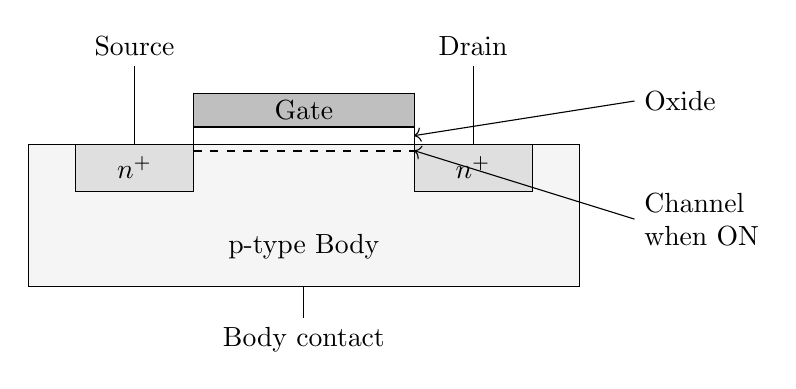
\begin{tikzpicture}[x=1cm,y=1cm]
\draw[fill=gray!8] (0,0) rectangle (7,1.8);
\draw[fill=gray!25] (0.6,1.2) rectangle (2.1,1.8);
\draw[fill=gray!25] (4.9,1.2) rectangle (6.4,1.8);
\node at (1.35,1.5) {$n^+$};\node at (5.65,1.5) {$n^+$};
\node at (3.5,0.5) {p-type Body};
\draw[fill=white] (2.1,1.8) rectangle (4.9,2.02);
\draw[fill=gray!50] (2.1,2.02) rectangle (4.9,2.45);
\node at (3.5,2.23) {Gate};
\draw (1.35,1.8)--(1.35,2.8) node[above] {Source};
\draw (5.65,1.8)--(5.65,2.8) node[above] {Drain};
\draw (3.5,0)--(3.5,-0.4) node[below] {Body contact};
\draw[<-] (4.9,1.91)--(7.7,2.35) node[right] {Oxide};
\draw[dashed,thick] (2.1,1.72)--(4.9,1.72);
\draw[<-] (4.9,1.72)--(7.7,0.85) node[right,align=left] {Channel\\when ON};
\end{tikzpicture}
\end{latin}
\caption{طرح آموزشی مقطع \lr{nMOS} بر پایه شکل \secnum{۱.۹} کتاب
\cite{weste}. خط‌چین محل تشکیل کانال را نشان می‌دهد؛ وجود همیشگی کانال را القا نمی‌کند.
خط اتصال بدنه فقط نمایش مفهومی پایانه است، نه طرح ساخت تماس.}
\label{fig:ch1-crosssection}
\end{figure}

در \lr{pMOS}، نوع ناحیه‌ها معکوس است: \lr{Source} و \lr{Drain} از نوع
\(p^+\) و بدنه از نوع \lr{n} هستند. در \lr{CMOS}، هر دو نوع روی یک تراشه
ساخته می‌شوند؛ به همین دلیل برای یکی از آن‌ها ناحیه مناسب \lr{Well} لازم است
\cite[صفحات چاپی ۷ و ۸]{weste}.
نام \lr{MOS} تاریخی است؛ جنس \lr{Gate} در دوره‌های مختلف یکسان نبوده است.

\subsection{تشکیل کانال در \lr{nMOS} و \lr{pMOS}}
برای \lr{nMOS} با بدنه و \lr{Source} نزدیک زمین، بالا بردن ولتاژ
\lr{Gate} الکترون‌ها را به سطح زیر عایق جذب می‌کند.
با ولتاژ کافی، نزدیک سطح کانالی با حامل غالب الکترون تشکیل می‌شود؛
این \lr{Inversion} مسیر هدایت میان دو ناحیه \(n^+\) را فراهم می‌کند
\cite[صفحه چاپی ۸]{weste}\cite[اسلایدهای ۶ و ۷]{mos}.
خاموش بودن یعنی مسیر کانال در مدل ساده برقرار نیست؛ این مدل جریان نشتی را حذف می‌کند.

در \lr{pMOS} با بدنه و \lr{Source} نزدیک تغذیه، پایین آوردن ولتاژ
\lr{Gate} نسبت به \lr{Source}، کانال حفره‌ای را ایجاد می‌کند.
بنابراین رفتار کنترلی آن مکمل \lr{nMOS} است.
این توصیف مقدماتی است؛ حالت‌های بار سطحی و روابط کمی در ابتدای فصل دوم استخراج می‌شوند.

\subsection{ولتاژ کنترل، آستانه و مدل \lr{Switch}}
برای \lr{nMOS} از اختلاف \(V_{gs}=V_g-V_s\) و آستانه مثبت \(V_{tn}\)
استفاده می‌کنیم. برای \lr{pMOS} در قرارداد اندازه‌های مثبت،
\(V_{sg}=V_s-V_g\) را با \(|V_{tp}|\) مقایسه می‌کنیم:
\begin{equation}\label{eq:ch1-threshold}
V_{gs}>V_{tn}\quad(\mathrm{nMOS}),\qquad
V_{sg}>|V_{tp}|\quad(\mathrm{pMOS}).
\end{equation}
در هر دو شرط، معیار اختلاف پتانسیل است، نه ولتاژ یک پایانه به‌تنهایی.
برابری با آستانه، مرز مدل ساده است؛ برای کاربرد عملی نمی‌توان آن را هدایت قوی دانست.
بدنه و آستانه نیز در مدل‌های دقیق‌تر مستقل از بایاس نیستند.

\textbf{مثال آموزشی.} در یک \lr{nMOS} فرضی با \(V_{tn}=\qty{0.3}{\volt}\)،
اگر \(V_g=\qty{1}{\volt}\) و \(V_s=\qty{0.9}{\volt}\)،
داریم \(V_{gs}=\qty{0.1}{\volt}\) و شرط روشن بودن برقرار نیست.
پس «\lr{Gate} بالا است» به‌تنهایی کافی نیست.
در گیت‌های ایستای متعارف که \lr{nMOS} خروجی را به زمین و \lr{pMOS} آن را
به تغذیه وصل می‌کند، ورودی‌های ریل‌به‌ریل این قاعده ساده را می‌دهند:
ورودی یک، \lr{nMOS} را روشن و \lr{pMOS} را خاموش می‌کند؛ ورودی صفر برعکس است
\cite[اسلاید ۲۱]{intro}. فرض می‌کنیم تغذیه از آستانه‌های لازم بیشتر است.

مدل \lr{Switch}، مسیر روشن را وصل و مسیر خاموش را قطع فرض می‌کند.
در آن، مقاومت مسیر، ظرفیت، نشتی و زمان روشن شدن را حذف می‌کنیم.
روشن بودن فقط امکان عبور جریان را نشان می‌دهد؛ بدون اختلاف ولتاژ یا بار مناسب،
جریان می‌تواند صفر باشد. شباهت تقریبی دو ناحیه \lr{Source} و \lr{Drain}
در شکل مقدماتی نیز مجوز نادیده گرفتن دیودهای بدنه یا محدودیت‌های یک قطعه واقعی نیست.

\subsection{پرسش کوتاه برای کنترل مدل}
\begin{enumerate}
\item \textbf{چرا \lr{Gate} عایق‌شده می‌تواند جریان کانال را کنترل کند؟}
کنترل با میدان الکتریکی و تغییر بار سطح انجام می‌شود؛ به عبور جریان اصلی از عایق نیاز ندارد.
\item \textbf{آیا بدون جریان رسانشی \lr{Gate}، ورودی هیچ انرژی نمی‌خواهد؟}
خیر؛ تغییر ولتاژ، ظرفیت ورودی را شارژ و دشارژ می‌کند.
\item \textbf{چرا بدنه را نباید حذف‌شده فرض کنیم؟}
پایانه چهارم بر پیوندها و آستانه اثر دارد؛ در این گام فقط اتصال متعارف و مدل ساده آن را به کار می‌بریم.
\end{enumerate}

% !TeX root = booklet-01.tex
\section{گیت‌های ایستای \lr{CMOS}}
\label{sec:book-cmos}
\label{sec:ch1-static}
\subsection{شبکه بالا و پایین چه وظیفه‌ای دارند؟}
گیت \lr{Static Complementary CMOS} یک شبکه \lr{pMOS} میان تغذیه و خروجی
به نام \lr{Pull-up Network (PUN)} و یک شبکه \lr{nMOS} میان خروجی و زمین
به نام \lr{Pull-down Network (PDN)} دارد.
برای ورودی‌های دودویی پایدار و در مدل \lr{Switch}، باید دقیقاً یکی از دو شبکه
مسیر برقرار داشته باشد \cite[بخش \secnum{۱.۴.۳}]{weste}.
این «دقیقاً یکی» هم از خروجی شناور و هم از مسیر مستقیم تغذیه به زمین جلوگیری می‌کند.

اگر شرط هدایت پایین را \(F\) بنامیم، خروجی وقتی \(F=1\) است صفر می‌شود.
پس \(Y=\overline{F}\)، و شبکه بالا باید شرط \(\overline{F}\) را پیاده کند.
\textbf{شرط هدایت شبکه پایین را نباید با تابع خروجی یکی گرفت.}
جدول \ref{tab:ch1-drive} چهار حالت کلی اتصال را نشان می‌دهد.
\begin{table}[ht]
\centering
\caption{حالت خروجی از روی هدایت دو شبکه در مدل مقدماتی؛ اثر گذرا و نشتی حذف شده است.}
\label{tab:ch1-drive}
\begin{tabular}{ccc}
\toprule
شبکه بالا & شبکه پایین & وضعیت خروجی\\
\midrule
قطع & وصل & صفر منطقی\\
وصل & قطع & یک منطقی\\
قطع & قطع & \lr{High Impedance} یا \(Z\)\\
وصل & وصل & \lr{Contention}\\
\bottomrule
\end{tabular}
\end{table}
در \(Z\)، خروجی از دو ریل جداست و مقدار آن ممکن است به بار قبلی وابسته باشد.
در \lr{Contention}، دو شبکه با هم خروجی را به دو ریل می‌کشند؛
مدل کلید ایدئال ولتاژ و جریان واقعی این اتصال را تعیین نمی‌کند.
نماد \(X\) در بحث مدار می‌تواند خروجی نامعین را نشان دهد؛
در جدول فشرده یک تابع، ممکن است به معنی «مقدار ورودی برای این سطر اهمیتی ندارد» باشد.
این دو کاربرد باید از متن تشخیص داده شوند \cite[صفحه چاپی ۱۰ و جدول بخش \secnum{۱.۴.۸}]{weste}.

\subsection{\lr{Inverter}: تحلیل اتصال، نه حفظ جدول}
در شکل \ref{fig:ch1-inverter}، ورودی \(A\) به \lr{Gate} هر دو ترانزیستور
و خروجی \(Y\) به \lr{Drain}های مشترک وصل است.
\lr{Source} بالا به \(V_{\mathrm{DD}}\) و پایین به زمین متصل است؛
بدنه‌ها نیز به‌ترتیب به تغذیه و زمین وصل‌اند و در نماد ساده رسم نشده‌اند.
\begin{figure}[ht]
\centering
\begin{latin}
\begin{circuitikz}[american]
\draw (0,2) node[pmos] (p) {} (0,-1) node[nmos] (n) {};
\draw (p.S)--(0,3.2) node[above] {$V_{\mathrm{DD}}$};
\draw (n.S)--(0,-2.2) node[ground] {};
\draw (p.D)--(0,0.5)--(n.D);
\draw (0,0.5) to[short,*-o] (1.8,0.5) node[right] {$Y$};
\draw (p.G)--(-1.6,2)--(-1.6,-1)--(n.G);
\draw (-1.6,0.5) to[short,*-o] (-2.5,0.5) node[left] {$A$};
\node[right] at (0.5,2) {pMOS};\node[right] at (0.5,-1) {nMOS};
\end{circuitikz}
\end{latin}
\caption{بازترسیم آموزشی \lr{Inverter} بر پایه شکل \secnum{۱.۱۱} کتاب و اسلاید ۲۳
\cite{weste,intro}. حباب \lr{Gate} ترانزیستور بالا نشانه \lr{pMOS} است.}
\label{fig:ch1-inverter}
\end{figure}

اگر \(A=0\)، پایین قطع و بالا وصل است؛ پس خروجی به تغذیه می‌رسد.
اگر \(A=1\)، بالا قطع و پایین وصل است؛ پس خروجی به زمین می‌رسد.
بنابراین \(Y=\overline{A}\). ورودی به خروجی اتصال رسانشی مستقیم ندارد؛
ورودی فقط وضعیت مسیرها را کنترل می‌کند.

اگر خروجی ظرفیت داشته باشد، برای رسیدن به ریل باید شارژ یا دشارژ شود.
از رابطه \(I=C\,\mathrm{d}V/\mathrm{d}t\) در بخش پیش‌نیازها می‌دانیم
این تغییر زمان می‌خواهد. مدل فعلی مقدار منطقی پایدار را می‌دهد، نه زمان گذار.
در ورودی میانی، فرض «دقیقاً یکی روشن است» لزوماً درست نیست؛
تحلیل آن به منحنی انتقال و ناحیه عملکرد جزوه سوم نیاز دارد.

\subsection{\lr{NAND}: سری در پایین، موازی در بالا}
برای دو \lr{nMOS} سری، جریان پایین فقط وقتی مسیر دارد که هر دو ورودی یک باشند؛
پس \(F_{\mathrm{PDN}}=AB\). خروجی در این حالت صفر می‌شود و تابع موردنظر
\(Y=\overline{AB}\) است. طبق \lr{De Morgan}:
\begin{equation}\label{eq:ch1-nand}
F_{\mathrm{PUN}}=\overline{AB}=\overline{A}+\overline{B}.
\end{equation}
هر \lr{pMOS} با صفر ورودی خودش روشن می‌شود، پس شبکه بالا باید دو \lr{pMOS}
موازی داشته باشد. در شکل \ref{fig:ch1-nand-nor}، مسیر هر ورودی را می‌توان دنبال کرد
\cite[بخش \secnum{۱.۴.۲}]{weste}\cite[اسلاید ۲۴]{intro}.

\begin{figure}[ht]
\centering
\begin{latin}
\begin{circuitikz}[american,scale=0.9,transform shape]
\begin{scope}
\draw (0,3) node[pmos] (pa) {} (2,3) node[pmos] (pb) {};
\draw (pa.S)--(0,4)--(2,4)--(pb.S);\node[above] at (1,4) {$V_{\mathrm{DD}}$};
\draw (pa.D)--(0,2)--(2,2)--(pb.D);
\draw (1,0.9) node[nmos] (na) {} (1,-0.8) node[nmos] (nb) {};
\draw (1,2)--(na.D) (na.S)--(nb.D) (nb.S)--(1,-1.8) node[ground] {};
\draw (2,2) to[short,*-o] (3,2) node[right] {$Y$};
\node[left] at (pa.G) {$A$};\node[left] at (pb.G) {$B$};
\node[left] at (na.G) {$A$};\node[left] at (nb.G) {$B$};
\node at (1,-2.5) {NAND};
\end{scope}
\begin{scope}[xshift=7cm]
\draw (1,3) node[pmos] (pc) {} (1,1.3) node[pmos] (pd) {};
\draw (pc.S)--(1,4) node[above] {$V_{\mathrm{DD}}$};\draw (pc.D)--(pd.S);
\draw (pd.D)--(1,0.3)--(0,0.3) (1,0.3)--(2,0.3);
\draw (0,-0.8) node[nmos] (nc) {} (2,-0.8) node[nmos] (nd) {};
\draw (0,0.3)--(nc.D) (2,0.3)--(nd.D);
\draw (nc.S)--(0,-1.8)--(2,-1.8)--(nd.S);\draw (1,-1.8) node[ground] {};
\draw (2,0.3) to[short,*-o] (3,0.3) node[right] {$Y$};
\node[left] at (pc.G) {$A$};\node[left] at (pd.G) {$B$};
\node[left] at (nc.G) {$A$};\node[left] at (nd.G) {$B$};
\node at (1,-2.5) {NOR};
\end{scope}
\end{circuitikz}
\end{latin}
\caption{بازترسیم دو گیت دوورودی بر پایه شکل‌های \secnum{۱.۱۲} و \secnum{۱.۱۶} کتاب
\cite{weste}. تکرار برچسب ورودی یعنی ولتاژ مشترک \lr{Gate}ها؛ سیم کنترل برای خوانایی حذف شده است.
بدنه همه \lr{nMOS}ها به زمین و بدنه همه \lr{pMOS}ها به تغذیه متصل است.}
\label{fig:ch1-nand-nor}
\end{figure}

برای ورودی‌های \((A,B)=(0,0)\)، هر دو \lr{pMOS} روشن‌اند و هر دو
\lr{nMOS} خاموش؛ خروجی یک می‌شود. در \((0,1)\)، مسیر پایین با ترانزیستور
کنترل‌شده با \(A\) قطع است و مسیر بالای مربوط به \(A\) وصل؛ باز خروجی یک است.
حالت \((1,0)\) مشابه است. فقط \((1,1)\) مسیر پایین را کامل و بالا را قطع می‌کند.
این چهار بررسی، جدول \ref{tab:ch1-gates} را می‌سازند.

\subsection{\lr{NOR} و تعمیم به چند ورودی}
در \lr{NOR} باید وقتی دست‌کم یک ورودی یک است، خروجی صفر شود؛
پس پایین دو \lr{nMOS} موازی با شرط \(A+B\) دارد.
بالا باید فقط وقتی هر دو ورودی صفرند هدایت کند، یعنی
\(\overline{A+B}=\overline{A}\,\overline{B}\)؛ پس دو \lr{pMOS} سری لازم است
\cite[بخش \secnum{۱.۴.۴}]{weste}\cite[اسلاید ۲۵]{intro}.
\begin{table}[ht]
\centering
\caption{خروجی پایدار دو گیت؛ هر دو برای چهار ترکیب ورودی کنترل شده‌اند.}
\label{tab:ch1-gates}
\begin{tabular}{cccc}
\toprule
\(A\)&\(B\)&\(Y_{\mathrm{NAND}}\)&\(Y_{\mathrm{NOR}}\)\\
\midrule
۰&۰&۱&۱\\
۰&۱&۱&۰\\
۱&۰&۱&۰\\
۱&۱&۰&۰\\
\bottomrule
\end{tabular}
\end{table}
برای \lr{NAND} با \(k\) ورودی، پایین \(k\) ترانزیستور سری و بالا \(k\)
ترانزیستور موازی دارد؛ برای \lr{NOR} جای سری و موازی عوض می‌شود.
تعداد کل، \(2k\) ترانزیستور است.
مثلاً \lr{NAND} سه‌ورودی \(Y=\overline{ABC}\) شش ترانزیستور دارد
\cite[اسلاید ۲۶]{intro}.
افزایش تعداد ورودی‌ها، مسیرها و ظرفیت‌ها را نیز تغییر می‌دهد؛
برابر بودن تابع منطقی مجوز نتیجه‌گیری درباره برابر بودن سرعت نیست.

\subsection{گیت \lr{Compound} و اصل \lr{Conduction Complements}}
برای ساخت گیت \(Y=\overline{AB+CD}\)، نخست عبارت داخل مکمل را
شرط هدایت پایین می‌گیریم:
\begin{equation}\label{eq:ch1-aoi}
F_{\mathrm{PDN}}=AB+CD,\qquad
F_{\mathrm{PUN}}=(\overline{A}+\overline{B})(\overline{C}+\overline{D}).
\end{equation}
پایین دو شاخه موازی دارد که هر شاخه شامل دو \lr{nMOS} سری است.
بالا، گروه موازی \(A,B\) از نوع \lr{pMOS} را با گروه موازی \(C,D\) سری می‌کنیم.
عملگرها تغییر کرده‌اند، ولی برچسب \lr{Gate} هر ترانزیستور همان ورودی اصلی است؛
برای هر \lr{pMOS}، مکمل بودن شرط هدایت از خود نوع ترانزیستور می‌آید.
این تبدیل سری به موازی و برعکس، \lr{Conduction Complements} نام دارد
\cite[بخش \secnum{۱.۴.۵} و شکل \secnum{۱.۱۸}]{weste}.

شکل \ref{fig:ch1-aoi} شبکه‌ها را بدون شلوغی نماد ترانزیستور نشان می‌دهد.
هر بلوک یک ترانزیستور با نوع و نام ورودی کنترل است؛ نقطه‌ها اتصال الکتریکی‌اند.
\begin{figure}[ht]
\centering
\begin{latin}
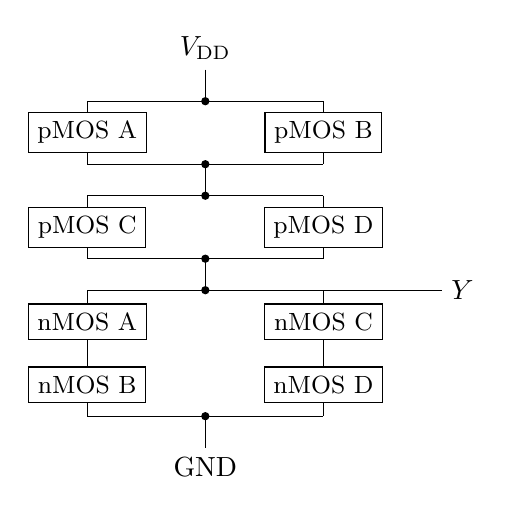
\begin{tikzpicture}[x=1cm,y=0.8cm]
\node[above] at (0,6) {$V_{\mathrm{DD}}$};
\draw (0,6)--(0,5.5)--(-1.5,5.5) (0,5.5)--(1.5,5.5);
\draw (-1.5,5.5)--(-1.5,4.5) node[midway,draw,fill=white,font=\small] {pMOS A};
\draw (1.5,5.5)--(1.5,4.5) node[midway,draw,fill=white,font=\small] {pMOS B};
\draw (-1.5,4.5)--(1.5,4.5);\draw (0,4.5)--(0,4)--(-1.5,4) (0,4)--(1.5,4);
\draw (-1.5,4)--(-1.5,3) node[midway,draw,fill=white,font=\small] {pMOS C};
\draw (1.5,4)--(1.5,3) node[midway,draw,fill=white,font=\small] {pMOS D};
\draw (-1.5,3)--(1.5,3);\draw (0,3)--(0,2.5)--(3,2.5) node[right] {$Y$};
\draw (0,2.5)--(-1.5,2.5)--(-1.5,1.5) node[midway,draw,fill=white,font=\small] {nMOS A};
\draw (0,2.5)--(1.5,2.5)--(1.5,1.5) node[midway,draw,fill=white,font=\small] {nMOS C};
\draw (-1.5,1.5)--(-1.5,0.5) node[midway,draw,fill=white,font=\small] {nMOS B};
\draw (1.5,1.5)--(1.5,0.5) node[midway,draw,fill=white,font=\small] {nMOS D};
\draw (-1.5,0.5)--(1.5,0.5);\draw (0,0.5)--(0,0) node[below] {GND};
\foreach \x/\y in {0/5.5,0/4.5,0/4,0/3,0/2.5,0/0.5} {\fill (\x,\y) circle (1.5pt);}
\end{tikzpicture}
\end{latin}
\caption{نمای توپولوژی آموزشی \lr{AOI22} برای رابطه \eqref{eq:ch1-aoi}.
بلوک‌های برچسب‌دار در این نمایش جایگزین نماد ترانزیستورند؛
وضعیت هدایت هر بلوک به نوع ترانزیستور و ورودی نوشته‌شده در آن بستگی دارد.}
\label{fig:ch1-aoi}
\end{figure}

نام \lr{AND-OR-Invert (AOI22)} می‌گوید دو گروه \lr{AND} دوورودی داریم،
خروجی آن‌ها \lr{OR} و سپس معکوس می‌شود.
در مثال \((A,B,C,D)=(1,1,0,0)\)، شاخه \(AB\) پایین وصل است؛
در بالا گروه \(A,B\) کاملاً قطع است، پس \(Y=0\).
در \((1,0,1,0)\)، هر شاخه پایین یک ترانزیستور قطع دارد؛
در بالا از \(B\) و \(D\) مسیر کامل داریم، پس \(Y=1\).
این دو مثال جای بررسی تمام حالت‌ها را نمی‌گیرند؛ رابطه مکمل، پوشش همه حالت‌ها را می‌دهد.

\textbf{مثال کتاب، \lr{OAI31}.} برای
\(Y=\overline{(A+B+C)D}\)، پایین گروه موازی \(A,B,C\) را با \(D\) سری می‌کنیم.
بالا گروه سری سه \lr{pMOS} با کنترل \(A,B,C\) را با یک \lr{pMOS} کنترل‌شده با \(D\)
موازی می‌کنیم؛ چون شرط بالا
\(\overline{A}\,\overline{B}\,\overline{C}+\overline{D}\) است.
این هشت ترانزیستور، تابع مثال \secnum{۱.۲} کتاب را می‌سازند
\cite[صفحه چاپی ۱۲]{weste}.

\subsection{چرا \lr{AND} را با یک \lr{NAND} و یک \lr{Inverter} می‌سازیم؟}
در خانواده محدود شبکه‌های مکمل ایستا که ورودی‌های غیرمعکوس مستقیماً
\lr{Gate}ها را کنترل می‌کنند، روشن شدن مسیر پایین خروجی را صفر می‌کند؛
ازاین‌رو گیت یک‌مرحله‌ای، تابع معکوس‌کننده ورودی‌هاست.
جابه‌جا کردن ساده \lr{nMOS} و \lr{pMOS} برای ساخت \lr{Buffer} مناسب نیست؛
با انتقال سطوح ضعیف روبه‌رو می‌شویم \cite[صفحه چاپی ۱۴]{weste}.
به‌جای آن، دو معکوس‌سازی می‌دهند
\[
 Y=\overline{\overline{AB}}=AB.
\]
برای \lr{OR} نیز \lr{NOR} و سپس \lr{Inverter} به کار می‌رود.

\lr{AND} دوورودی با این روش شش ترانزیستور دارد: چهار برای \lr{NAND}
و دو برای \lr{Inverter}. ساخت تابع \lr{AOI22} از دو \lr{AND}، یک \lr{OR}
و یک \lr{Inverter} با این سلول‌های ساده، \(6+6+6+2=20\)
ترانزیستور می‌خواهد؛ گیت \lr{Compound} فقط هشت ترانزیستور دارد.
این مقایسه شمارش قطعات است؛ برای نتیجه قطعی درباره \lr{Delay} یا توان باید
اندازه ترانزیستورها، بار و مسیرها نیز تحلیل شوند \cite[شکل \secnum{۱.۲۴}]{weste}.

\subsection{کنترل اعتبار گیت ایستا}
برای هر ترکیب ورودی، ابتدا قطع یا وصل بودن تک‌تک قطعات و سپس وجود مسیر کامل
را مشخص می‌کنیم. اگر پایین هدایت دارد، بالا باید قطع باشد و برعکس.
این کنترل برای تمام ورودی‌ها، شرط منطقی طراحی است.
در مدل ایدئال پایدار، ابعاد ترانزیستورها جدول درستی را عوض نمی‌کنند؛
در مدار واقعی، ابعاد بر زمان و توان و رفتار گذرا اثر دارند.
عبارت «توان ساکن صفر» نیز فقط به مدل بدون نشتی و ورودی‌های پایدار معتبر تعلق دارد؛
بار خازنی و هدایت هم‌زمان در گذار، همچنان انرژی مصرف می‌کنند.

\BookletSubsections{notes/booklet-01/ch1-pass-mux}
\BookletSubsections{notes/booklet-01/ch1-storage}
\section{ساخت و \lr{Layout} مدارهای \lr{CMOS}}
\label{sec:book-fabrication}
این بخش، زیربخش‌های \secnum{۱.۵.۱} تا \secnum{۱.۵.۵} کتاب را پوشش می‌دهد.
فرآیند \lr{n-well CMOS} و قواعد هندسی، مدل آموزشی مرجع هستند.
\BookletSubsections{notes/booklet-01/ch1-fabrication}
\BookletSubsections{notes/booklet-01/ch1-layout-rules}
\BookletSubsections{notes/booklet-01/ch1-layout-examples}
% !TeX root = booklet-01.tex
\section{تقسیم طراحی و سطوح \lr{Abstraction}}
\label{sec:book-partitioning}
\subsection{چرا طراحی بزرگ را تقسیم می‌کنیم؟}
خواندن یک \lr{Inverter} با دنبال کردن دو ترانزیستور ممکن بود؛
در یک پردازنده، بررسی هم‌زمان تمام ترانزیستورها روش مناسبی برای فهم عملکرد نیست.
\lr{Abstraction} یعنی جزئیات نامربوط به پرسش فعلی را موقتاً پنهان کنیم،
ولی قرارداد ورودی، خروجی و رفتار را نگه داریم.
\lr{Design Partitioning} نیز تقسیم سیستم به بخش‌هایی با مسئولیت و رابط مشخص است
\cite[بخش \secnum{۱.۶}]{weste}.

تقسیم بیش‌ازحد مستقل، ممکن است هر بلوک را بهینه ولی ترکیب کل را نامناسب کند؛
وابستگی همه بلوک‌ها به همه جزئیات یکدیگر نیز پیشرفت را کند می‌کند.
برای مثال، کوچک کردن یک بلوک با خروجی ضعیف می‌تواند نیاز به بافر و تاخیر بلوک بعدی را بیشتر کند.
پس بهینه‌سازی باید اثر بر همسایه‌ها و هدف کل سیستم را نیز بسنجد.

\subsection{پنج سطح طراحی را با یک مثال تشخیص دهیم}
جدول \ref{tab:design-levels} پنج سطح بخش \secnum{۱.۶.۱} کتاب را روی مثال
جمع دو داده نشان می‌دهد \cite{weste}\cite[اسلاید ۱۷]{intro}.
ستون پرسش، دلیل متفاوت بودن سطح‌ها را مشخص می‌کند.
\begin{table}[ht]
\centering
\caption{سطوح طراحی و نمونه تصمیم در هر سطح}
\label{tab:design-levels}
\begin{tabularx}{\textwidth}{l>{\raggedleft\arraybackslash}X>{\raggedleft\arraybackslash}X}
\toprule
سطح & پرسش اصلی & نمونه تصمیم\\
\midrule
\lr{Architecture}&کار قابل مشاهده سیستم چیست؟&دستور جمع، ثبات‌های قابل مشاهده و معنای نتیجه\\
\lr{Microarchitecture}&عملیات با چه منابعی و در چه چرخه‌هایی انجام می‌شود؟&یک \lr{ALU} مشترک یا چند واحد؛ محل ثبات‌های میانی\\
\lr{Logic}&واحدها از چه منطق و حالت‌هایی ساخته می‌شوند؟&جمع‌کننده \lr{Ripple Carry} یا \lr{Carry Lookahead}\\
\lr{Circuit}&منطق با چه مدار ترانزیستوری پیاده می‌شود؟&گیت‌های \lr{Static CMOS} یا مدار عبوری\\
\lr{Physical}&اجزا و اتصال‌ها کجا و با چه هندسه‌ای قرار می‌گیرند؟&جانمایی سلول و مسیر فلزی\\
\bottomrule
\end{tabularx}
\end{table}

دو پیاده‌سازی می‌توانند دستورهای یکسانی اجرا کنند ولی تعداد چرخه، مصرف توان
و مساحت متفاوت داشته باشند. بنابراین \lr{Architecture} با
\lr{Microarchitecture} یکی نیست. همچنین انتخاب الگوریتم جمع‌کننده با انتخاب
مدار ترانزیستوری گیت آن یک تصمیم نیست.
\lr{ALU} مخفف \lr{Arithmetic/Logic Unit} است و عملیات حسابی و منطقی را انجام می‌دهد.

این سطح‌ها دیوار مستقل نیستند. اگر یک مسیر فیزیکی طولانی شود، ممکن است
هدف فرکانس برآورده نشود و تعداد مرحله‌های زمانی یا ساختار منطقی تغییر کند.
کتاب بر تعامل طراحی \lr{Microarchitecture}، منطق، مدار و شکل فیزیکی تاکید می‌کند؛
ترتیب توضیح آموزشی، تضمین یک فرایند یک‌طرفه و بدون بازگشت نیست.

\subsection{چهار اصل \lr{Structured Design}}
\begin{enumerate}
\item \textbf{\lr{Hierarchy}:} سیستم به بلوک، زیر‌بلوک و سلول تقسیم می‌شود.
برای مثال پردازنده شامل \lr{Datapath} و کنترل است؛ جمع‌کننده داخل \lr{Datapath}
نیز از \lr{Full Adder}ها ساخته می‌شود.
\item \textbf{\lr{Regularity}:} تعداد نوع‌های متفاوت بلوک کم و استفاده مجدد زیاد باشد.
هشت نمونه یک \lr{MUX} تک‌بیتی، منطق انتخاب هشت‌بیتی را می‌سازند؛
لازم نیست هر بیت از ابتدا با سبک متفاوت طراحی شود.
\item \textbf{\lr{Modularity}:} رابط بلوک روشن باشد؛ عرض داده، قطبیت کنترل،
زمان معتبر بودن و بار قابل راه‌اندازی جزو قراردادند.
نام برابر دو سیگنال یا اتصال سیم به‌تنهایی، سازگاری رابط را اثبات نمی‌کند.
\item \textbf{\lr{Locality}:} اطلاعات در زمان و مکان نزدیک استفاده‌اش نگه داشته شود.
قرار دادن ثبات موقت نزدیک واحد محاسبه می‌تواند نیاز به رفت‌وآمد داده را کمتر کند؛
نتیجه کمی آن به سیم‌کشی و مدل مدار وابسته است.
\end{enumerate}
این اصول از بخش \secnum{۱.۶.۲} کتاب و اسلاید ۱۶ گرفته شده‌اند
\cite{weste,intro}. تکرار یک سلول بررسی‌شده، تعداد مسئله‌های مستقل را کم می‌کند؛
اما اتصال و زمان‌بندی نمونه‌های کنار هم هنوز باید کنترل شوند.

\subsection{سه دامنه \lr{Behavioral}، \lr{Structural} و \lr{Physical}}
سطح \lr{Abstraction} میزان جزئیات را می‌گوید؛ دامنه، نوع توصیف را.
در نمودار \lr{Y}، سه دامنه در چند سطح جزئیات وجود دارند
\cite[بخش \secnum{۱.۶.۳} و شکل \secnum{۱.۴۸}]{weste}:
\lr{Behavioral} می‌گوید «چه می‌کند»، \lr{Structural} می‌گوید «از چه اجزایی و اتصال‌هایی ساخته شده»
و \lr{Physical} هندسه و جای اجزا را توصیف می‌کند.

برای یک \lr{Full Adder}، رابطه جمع و نقلی توصیف رفتاری است؛
شبکه \lr{XOR} و گیت‌های نقلی توصیف ساختاری است؛
مستطیل‌های لایه‌ها و تماس‌ها توصیف فیزیکی‌اند.
پس \lr{Behavioral} فقط مخصوص سطح پردازنده و \lr{Physical} فقط مخصوص یک ترانزیستور نیست؛
یک تراشه نیز \lr{Floorplan} فیزیکی دارد.

در شکل \ref{fig:design-domains}، خط‌های بین دامنه‌ها تبدیل توصیف را نشان می‌دهند.
پس از هر تبدیل باید معادل بودن رفتار موردنظر بررسی شود؛
هندسه کوچک یا خروجی ابزار خودکار به‌خودی‌خود حفظ عملکرد را ثابت نمی‌کند.
\begin{figure}[ht]
\centering
\begin{latin}
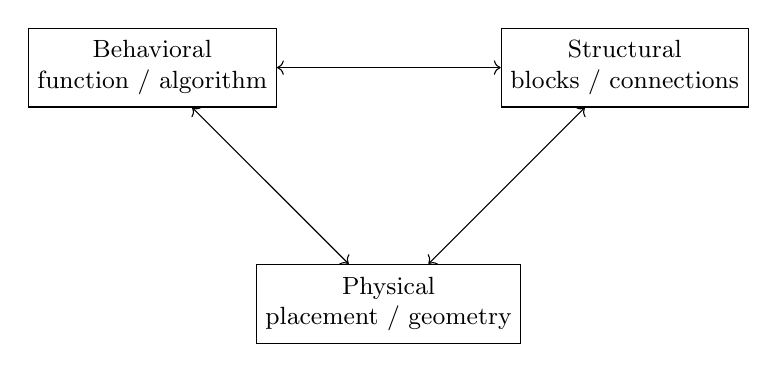
\begin{tikzpicture}[font=\small]
\node[draw,align=center,minimum width=3.1cm,minimum height=1cm] (b) at (-3,1.6) {Behavioral\\function / algorithm};
\node[draw,align=center,minimum width=3.1cm,minimum height=1cm] (s) at (3,1.6) {Structural\\blocks / connections};
\node[draw,align=center,minimum width=3.1cm,minimum height=1cm] (p) at (0,-1.4) {Physical\\placement / geometry};
\draw[<->] (b)--(s);\draw[<->] (b)--(p);\draw[<->] (s)--(p);
\end{tikzpicture}
\end{latin}
\caption{بازنمایی مفهومی رابطه سه دامنه، بر پایه بحث نمودار \lr{Y} کتاب
\cite{weste}. این شکل بازتولید هندسی خود نمودار \lr{Y} نیست؛
تبدیل دامنه‌ها در یک سطح مشخص را برجسته می‌کند.}
\label{fig:design-domains}
\end{figure}

\subsection{مثال بررسی رابط}
فرض کنید بلوکی \lr{MUX} هشت‌بیتی دارد و انتخابش با یک بیت \(S\) انجام می‌شود.
باید معلوم باشد \(S=0\) کدام ورودی را انتخاب می‌کند، هر ورودی چه زمانی معتبر است
و خروجی چه زمانی مصرف می‌شود. اتصال ورودی هفت‌بیتی به آن، یا برداشت معکوس از
معنای \(S\)، می‌تواند عملکرد را عوض کند؛ حتی اگر نام بلوک درست باشد.
در ادامه، همین انضباط را برای رابط پردازنده و حافظه به کار می‌بریم.

\section{مثال پردازنده آموزشی \lr{MIPS}}
\label{sec:book-mips}
در زیرمجموعه آموزشی کتاب، داده و \lr{PC} هشت‌بیتی و دستور ۳۲ بیتی است.
هر جا قرارداد با معماری کامل متفاوت باشد، فرض مثال در متن مشخص می‌شود.
\BookletSubsections{notes/booklet-01/ch1-mips-architecture}
\BookletSubsections{notes/booklet-01/ch1-mips-microarchitecture}
\section{از رابط بلوک‌ها تا \lr{Logic Design} و \lr{HDL}}
\label{sec:book-logic-design}
\BookletSubsections{notes/booklet-01/ch1-logic-hdl}
\section{طراحی در سطح مدار}
\label{sec:book-circuit-design}
\subsection{جریان و خازن چگونه تأخیر را تعیین می‌کنند؟}
در \lr{Circuit Design}، برای تابع منطقی مشخص، شبکه ترانزیستورها و اندازه آن‌ها
انتخاب می‌شود. خروجی یک گیت، ورودی گیت بعدی و سیم میان آن‌ها را راه‌اندازی می‌کند.
عایق \lr{Gate} موجب رفتار خازنی ورودی است. خازن‌های \lr{Diffusion} و سیم نیز به بار
خروجی افزوده می‌شوند. بنابراین صفر و یک‌شدن خروجی به جابه‌جایی بار الکتریکی نیاز دارد
\cite[بخش \secnum{۱.۹}، شکل \secnum{۱.۶۰}]{weste}.

اگر خازن معادل بار را \(C_L\) بنامیم، در مدل خازن ثابت رابطه بار و ولتاژ
\(Q=C_LV\) است. با تغییر ولتاژ به اندازه \(\Delta V\)، بار به اندازه
\(\Delta Q=C_L\Delta V\) تغییر می‌کند. جریان متوسط، بار جابه‌جاشده تقسیم بر زمان است.
از این دو تعریف، بدون نیاز به حل معادله دیفرانسیل، داریم
\begin{equation}
 I_{\mathrm{avg}}=\frac{\Delta Q}{\Delta t}
 \quad\Longrightarrow\quad
 \Delta t=\frac{C_L\Delta V}{I_{\mathrm{avg}}}.
 \label{eq:impl-charge-delay}
\end{equation}
برای جریان لحظه‌ای همین معنا به صورت \(i=C_L\,dV/dt\) نوشته می‌شود.
نماد \(dV/dt\) سرعت تغییر ولتاژ را بیان می‌کند. برای تخمین زمان تغییر کامل ولتاژ
از صفر تا \(V_{DD}\)، کتاب از تقریب
\begin{equation}
 t_{\mathrm{sw}}\approx\frac{C_LV_{DD}}{I_{\mathrm{avg}}}
 \label{eq:impl-full-swing}
\end{equation}
استفاده می‌کند. جریان ترانزیستور در طول گذار تغییر می‌کند، بنابراین انتخاب
\(I_{\mathrm{avg}}\) باید با همان بازه ولتاژ سازگار باشد. \lr{Propagation Delay}
معمولاً میان نقاط مرجع گذار ورودی و خروجی، مانند نصف ولتاژ تغذیه، اندازه‌گیری می‌شود.
رابطه \eqref{eq:impl-full-swing} یک تخمین مرتبه اول برای زمان تغییر ولتاژ است.

کنترل واحدها نتیجه را روشن می‌کند. چون \(\unit{\farad}=\unit{\coulomb\per\volt}\)
و \(\unit{\ampere}=\unit{\coulomb\per\second}\)، واحد
\(C_LV/I\) برابر ثانیه می‌شود. بار بیشتر، زمان بیشتر می‌خواهد. جریان قوی‌تر همان بار
را سریع‌تر جابه‌جا می‌کند. در مدل ایدئال، اگر \(C_L=0\) باشد این سهم از تأخیر صفر
می‌شود. اگر جریان به صفر نزدیک شود، زمان لازم افزایش می‌یابد.

در مثال فرضی، \(C_L=\qty{20}{\femto\farad}\)، \(V_{DD}=\qty{1}{\volt}\)
و \(I_{\mathrm{avg}}=\qty{100}{\micro\ampere}\) هستند. جای‌گذاری مرحله‌ای می‌دهد
\begin{equation*}
 t_{\mathrm{sw}}\approx
 \frac{20\times10^{-15}\times1}{100\times10^{-6}}\,\unit{\second}
 =2\times10^{-10}\,\unit{\second}=\qty{200}{\pico\second}.
\end{equation*}
دوبرابرشدن بار با جریان ثابت، زمان را به \qty{400}{\pico\second} می‌رساند.
این اعداد صرفاً برای تمرین تبدیل پیشوند و تحلیل رابطه انتخاب شده‌اند.

\subsection{اثر عرض ترانزیستور و بار مرحله بعد}
با ثابت‌بودن طول و شرایط بایاس، مدل مقدماتی جریان و خازن ورودی را متناسب با عرض
\(W\) می‌گیرد \cite[صفحه ۴۲]{weste}. افزایش عرض، جریان راه‌انداز و هم‌زمان بار
دیده‌شده در مرحله قبل را افزایش می‌دهد. اگر ضریب بزرگ‌کردن ترانزیستور \(s>0\)
باشد، برای تحلیل ساده می‌توان نوشت
\begin{equation}
 I(s)\approx sI_0,\qquad
 C_L(s)\approx C_{\mathrm{ext}}+sC_{\mathrm{int},0},\qquad
 t(s)\approx\frac{V_{DD}}{I_0}
 \left(\frac{C_{\mathrm{ext}}}{s}+C_{\mathrm{int},0}\right).
 \label{eq:impl-sizing}
\end{equation}
در این مدل، \(C_{\mathrm{ext}}\) بار ثابت خارجی و \(C_{\mathrm{int},0}\) سهم داخلی
در اندازه اولیه است. بزرگ‌کردن گیت، سهم بار ثابت را سریع‌تر راه‌اندازی می‌کند، اما
سهم خازن داخلی نیز رشد می‌کند. خازن ورودی بزرگ‌تر، تأخیر و انرژی مرحله قبل را تغییر
می‌دهد. انتخاب اندازه به مسیر چندمرحله‌ای، \lr{Fan-in}، \lr{Fan-out}، سیم و محدودیت
مساحت وابسته است. مدل‌های دقیق‌تر جریان و خازن در فصل ۲ و روش‌های اندازه‌گذاری در فصل ۴ آمده‌اند.

\subsection{استخراج انرژی و توان از شارژ خازن}
توان لحظه‌ای منبع تغذیه برابر \(p=V_{DD}i\) است. برای شارژ کامل یک خازن از صفر
تا \(V_{DD}\)، منبع بار \(Q=C_LV_{DD}\) تحویل می‌دهد. چون ولتاژ منبع ثابت است،
انرژی دریافت‌شده از منبع برابر می‌شود با
\begin{equation}
 E_{\mathrm{supply}}=V_{DD}Q=C_LV_{DD}^2.
 \label{eq:impl-supply-energy}
\end{equation}
انرژی ذخیره‌شده در خود خازن از جمع انرژی‌های کوچک \(V\,dQ\) به دست می‌آید.
با \(dQ=C_L\,dV\)، مساحت زیر خط \(C_LV\) از صفر تا \(V_{DD}\) یک مثلث است، پس
\begin{equation}
 E_C=\int_0^{V_{DD}}C_LV\,dV=\frac12 C_LV_{DD}^2.
 \label{eq:impl-stored-energy}
\end{equation}
در شارژ معمول مقاومتی، نیم دیگر انرژی منبع در مسیر شارژ تلف می‌شود. هنگام تخلیه،
انرژی ذخیره‌شده نیز در مسیر تخلیه تلف می‌شود. بنابراین انرژی یک چرخه کامل
\(0\rightarrow1\rightarrow0\) در این مدل برابر \(C_LV_{DD}^2\) است.

اگر در هر ثانیه \(f_{\mathrm{cyc}}\) چرخه کامل رخ دهد، توان متوسط برابر انرژی
هر چرخه ضرب‌در تعداد چرخه در ثانیه خواهد بود
\begin{equation}
 P_{\mathrm{dyn}}=C_LV_{DD}^2f_{\mathrm{cyc}}.
 \label{eq:impl-dynamic-power}
\end{equation}
این همان صورت رابطه کتاب است \cite[صفحه ۴۳]{weste}. برای ارتباط با \lr{Clock}،
\(\alpha_{01}\) را متوسط تعداد گذارهای \(0\rightarrow1\) در هر دوره \lr{Clock}
تعریف می‌کنیم. در حالت پایدار، فرکانس شارژ \(\alpha_{01}f_{\mathrm{clk}}\) است، پس
\begin{equation}
 P_{\mathrm{dyn}}=\alpha_{01}C_LV_{DD}^2f_{\mathrm{clk}}.
 \label{eq:impl-activity-power}
\end{equation}
با شمارش مجموع گذارهای صعودی و نزولی، باید تعریف ضریب فعالیت را نیز عوض کرد.
برای سیگنال متناوب \(0,1,0,1,\ldots\) در نمونه‌های متوالی \lr{Clock}، در هر دو
دوره یک شارژ رخ می‌دهد، بنابراین \(\alpha_{01}=1/2\) است. برای چند گره، سهم
\(\alpha_{01,k}C_kV_{DD}^2f_{\mathrm{clk}}\) هر گره جمع می‌شود.

در مثال فرضی \(C_L=\qty{20}{\femto\farad}\)، \(V_{DD}=\qty{1}{\volt}\)،
\(f_{\mathrm{clk}}=\qty{100}{\mega\hertz}\) و \(\alpha_{01}=0.25\)، داریم
\begin{equation}
 P_{\mathrm{dyn}}=0.25(20\times10^{-15})(1)^2(100\times10^6)
 \,\unit{\watt}=\qty{0.50}{\micro\watt}.
 \label{eq:impl-power-example}
\end{equation}
کاهش ولتاژ به \qty{0.8}{\volt} با ثابت‌فرض‌کردن سایر عوامل، توان را در
\(0.8^2=0.64\) ضرب می‌کند و به \qty{0.32}{\micro\watt} می‌رساند. جریان ترانزیستور
نیز به ولتاژ وابسته است، پس بررسی سرعت به مدل جریان نیاز دارد.

\subsection{توان \lr{Static} و انتخاب پیاده‌سازی}
ترانزیستور خاموش واقعی جریان نشتی دارد. اگر جریان متوسط مستقیم از تغذیه به زمین
را \(I_{\mathrm{static}}\) بنامیم، از تعریف توان به دست می‌آید
\begin{equation}
 P_{\mathrm{static}}=V_{DD}I_{\mathrm{static}}.
 \label{eq:impl-static-power}
\end{equation}
این رابطه حتی در نبود تغییر منطقی خروجی کاربرد دارد \cite[صفحه ۴۳]{weste}.
برای جریان فرضی \qty{10}{\nano\ampere} و تغذیه \qty{1}{\volt}، توان
\qty{10}{\nano\watt} است. مجموع این سهم و مثال \eqref{eq:impl-power-example}،
در مدل دو مؤلفه‌ای، \qty{0.51}{\micro\watt} می‌شود. جریان گذرای هم‌پوشانی روشن‌شدن
شبکه‌های \lr{Pull-up} و \lr{Pull-down} نیز می‌تواند سهم دیگری ایجاد کند که در تحلیل
تفصیلی فصل توان بررسی می‌شود.

\lr{Synthesis} با انتخاب گیت‌های کتابخانه و اندازه آن‌ها، تابع منطقی را تحت
محدودیت‌های طراحی پیاده می‌کند. \lr{Custom Circuit Design} امکان انتخاب شبکه
ترانزیستوری متناسب با تابع را فراهم می‌سازد. کتاب اهمیت آن را برای بخش‌های دارای
نیاز سرعت یا توان ویژه و برای حجم تولید توجیه‌کننده هزینه مهندسی توضیح می‌دهد.
\lr{Area}، توان، سرعت و تلاش طراحی باید هم‌زمان سنجیده شوند.

\subsection{مثال \lr{Carry} با ۲۶ و ۱۲ ترانزیستور}
در \lr{Full Adder}، ورودی‌های تک‌بیتی \(a,b,c\) هستند و \(c\) نقش \lr{Carry-in}
را دارد. خروجی \(c_{\mathrm{out}}\) وقتی یک می‌شود که دست‌کم دو ورودی یک باشند.
تابع آن برابر است با
\begin{equation}
 c_{\mathrm{out}}=ab+ac+bc.
 \label{eq:impl-carry-majority}
\end{equation}
در این معادله، کنارهم‌نوشتن نمادها به معنای \lr{AND} و علامت جمع به معنای
\lr{OR} است. برای مثال \(a=b=1\) با هر مقدار \(c\)، خروجی یک می‌دهد.
اگر فقط یک ورودی یک باشد، هر سه حاصل‌ضرب صفر می‌شوند.

پیاده‌سازی شکل \secnum{۱.۶۱} کتاب از سه \lr{AND2} و یک \lr{OR3} تشکیل می‌شود
\cite{weste}. \lr{AND2} در \lr{Static CMOS} معمول، یک \lr{NAND2} چهارترانزیستوری
و یک \lr{Inverter} دوترانزیستوری دارد. \lr{OR3} نیز از \lr{NOR3} شش‌ترانزیستوری
و یک \lr{Inverter} ساخته می‌شود. بنابراین
\begin{equation*}
 N_{\mathrm{gate}}=3(4+2)+(6+2)=26.
\end{equation*}
مسیر ورودی تا خروجی از چهار مرحله وارون‌کننده منطقی عبور می‌کند.
تأخیر هر مرحله تابع اندازه و بار آن است.

برای ساخت مدار فشرده، ابتدا تابع را عامل‌گیری می‌کنیم
\begin{equation}
 F=ab+c(a+b),\qquad c_n=\overline F,\qquad c_{\mathrm{out}}=\overline{c_n}.
 \label{eq:impl-factored-carry}
\end{equation}
شبکه \lr{Pull-down} گره \(c_n\)، یک شاخه دوترانزیستوری سری با کنترل \(a,b\)
و یک شاخه شامل \(c\) در سری با دو ترانزیستور موازی \(a,b\) دارد. این شبکه پنج
\lr{nMOS} می‌خواهد. هرگاه \(F=1\) باشد، مسیری تا زمین برقرار می‌شود.

شبکه \lr{Pull-up} شکل کتاب نیز پنج \lr{pMOS} دارد. شرط هدایت آن را با
\(\bar a,\bar b,\bar c\) بیان می‌کنیم، زیرا \lr{pMOS} با ورودی صفر روشن می‌شود.
با قانون \lr{De Morgan} و توزیع حاصل‌ضرب داریم
\begin{align*}
 \overline F
 &=(\bar a+\bar b)(\bar c+\bar a\bar b)\\
 &=\bar c(\bar a+\bar b)+\bar a\bar b.
\end{align*}
جمله اول، \(c\) در سری با موازی \(a,b\)، و جمله دوم، سری \(a,b\) در شبکه
\lr{pMOS} را مشخص می‌کند. بنابراین برای هر ورودی دودویی پایدار، یکی از شبکه‌ها
گره \(c_n\) را به تغذیه مناسب می‌رساند. \lr{Inverter} پایانی دو ترانزیستور دیگر دارد
و تعداد کل \(5+5+2=12\) می‌شود. مسیر منطقی شامل یک گیت مرکب و یک
\lr{Inverter} است. مقایسه سرعت عددی، به اندازه ترانزیستورها و بارها نیاز دارد.

جدول \ref{tab:impl-carry} همه حالت‌های دودویی را کنترل می‌کند. ستون \lr{PDN}
و \lr{PUN}، وجود مسیر رسانا برای گره \(c_n\) را نشان می‌دهند.
\begin{table}[ht]
\centering
\caption{کنترل کامل تابع و شبکه‌های \lr{Carry} در مدل سوئیچی ایدئال.}
\label{tab:impl-carry}
\begin{tabular}{ccccccc}
\toprule
\(a\)&\(b\)&\(c\)&\lr{PDN}&\lr{PUN}&\(c_n\)&\(c_{\mathrm{out}}\)\\
\midrule
۰&۰&۰&۰&۱&۱&۰\\
۰&۰&۱&۰&۱&۱&۰\\
۰&۱&۰&۰&۱&۱&۰\\
۰&۱&۱&۱&۰&۰&۱\\
۱&۰&۰&۰&۱&۱&۰\\
۱&۰&۱&۱&۰&۰&۱\\
۱&۱&۰&۱&۰&۰&۱\\
۱&۱&۱&۱&۰&۰&۱\\
\bottomrule
\end{tabular}
\end{table}

\subsection{\lr{Schematic} و دو سطح \lr{Netlist}}
\lr{Schematic} اتصال‌ها را به صورت تصویر و \lr{Netlist} همان ارتباط‌ها را به صورت
متن نمایش می‌دهد. در توصیف ساختاری گیت‌ها، نمونه آموزشی تابع \lr{Carry} چنین است
\cite[صفحات ۴۳ و ۴۴]{weste}.
\begin{latin}
\small
\begin{verbatim}
module carry(input logic a, b, c, output logic cout);
  logic x, y, z;
  and g1(x, a, b);
  and g2(y, a, c);
  and g3(z, b, c);
  or  g4(cout, x, y, z);
endmodule
\end{verbatim}
\end{latin}
در این \lr{Verilog}، نخستین آرگومان هر گیت خروجی است. نام‌های \code{g1} تا
\code{g4} شناسه نمونه‌ها و \code{x}، \code{y} و \code{z} سیم‌های میانی هستند.
گیت عمومی هنوز اندازه، خازن و مدل فناوری را مشخص نمی‌کند.

در توصیف سوئیچی کتاب، \code{tranif1} با کنترل یک و \code{tranif0} با کنترل صفر
اتصال برقرار می‌کنند. ترتیب آرگومان آن‌ها دو پایانه مسیر و سپس کنترل است.
برای نمونه \code{tranif1 n3(cn, i1, c)} گره‌های \code{cn} و \code{i1} را هنگام
یک‌بودن \code{c} وصل می‌کند. مسیر در این مدل دوطرفه است. \code{supply0} و
\code{supply1} به‌ترتیب زمین و تغذیه منطقی، و \code{tri} گره سیمی با قابلیت حالت
پرامپدانس را معرفی می‌کنند. این نمایش برای بررسی اتصال و عملکرد سوئیچی مناسب است.

برای تحلیل پیوسته ولتاژ، جریان، تأخیر و توان، \lr{SPICE} به مدل افزاره و ابعاد نیاز
دارد. ترانزیستور \lr{MOS} چهار پایانه \lr{Drain}، \lr{Gate}، \lr{Source} و
\lr{Body} دارد. خط معرفی آن در کتاب به ترتیب زیر است
\cite[صفحات ۴۴ و ۴۵]{weste}.
\begin{latin}
\small
\begin{verbatim}
Mname drain gate source body model W=width L=length
+ AD=drain_area AS=source_area
Cname node1 node2 value
\end{verbatim}
\end{latin}
علامت \code{+} در آغاز خط، ادامه همان دستور را نشان می‌دهد. \code{W} و
\code{L} عرض و طول کانال، و \code{AD} و \code{AS} مساحت‌های اتصال
\lr{Drain} و \lr{Source} هستند. نام مدل، پارامترهای فناوری را به نمونه مرتبط می‌کند.
این ترتیب با ترتیب آرگومان گیت‌های \lr{Verilog} تفاوت دارد.

فهرست \lr{SPICE} آموزشی زیر اتصال و ابعاد مثال کتاب را حفظ می‌کند. پسوندهای
\code{u}، \code{p} و \code{f} به‌ترتیب ضرایب \(10^{-6}\)، \(10^{-12}\) و
\(10^{-15}\) هستند. بنابراین \code{W=2u} طول \qty{2}{\micro\metre} و
\code{AD=1.8p} مساحت \qty{1.8}{\micro\metre\squared} را مشخص می‌کنند.
نام‌های گره و ترتیب درگاه‌ها از مرجع حفظ شده‌اند.
\begin{latin}
\footnotesize
\begin{verbatim}
.SUBCKT CARRY A B C COUT VDD GND
MN1 I1 A GND GND NMOS W=2u L=0.6u AD=1.8p AS=3p
MN2 I1 B GND GND NMOS W=2u L=0.6u AD=1.8p AS=3p
MN3 CN C I1 GND NMOS W=2u L=0.6u AD=3p AS=3p
MN4 I2 B GND GND NMOS W=2u L=0.6u AD=0.9p AS=3p
MN5 CN A I2 GND NMOS W=2u L=0.6u AD=3p AS=0.9p
MP1 I3 A VDD VDD PMOS W=4u L=0.6u AD=3.6p AS=6p
MP2 I3 B VDD VDD PMOS W=4u L=0.6u AD=3.6p AS=6p
MP3 CN C I3 VDD PMOS W=4u L=0.6u AD=6p AS=6p
MP4 I4 B VDD VDD PMOS W=4u L=0.6u AD=1.8p AS=6p
MP5 CN A I4 VDD PMOS W=4u L=0.6u AD=6p AS=1.8p
MN6 COUT CN GND GND NMOS W=4u L=0.6u AD=6p AS=6p
MP6 COUT CN VDD VDD PMOS W=8u L=0.6u AD=12p AS=12p
CI1 I1 GND 6f
CI3 I3 GND 9f
CA A GND 12f
CB B GND 12f
CC C GND 6f
CCN CN GND 12f
CCOUT COUT GND 6f
.ENDS CARRY
\end{verbatim}
\end{latin}
در نمونه \code{MN3}، \lr{Body} به زمین متصل است، هرچند \lr{Source} روی گره
داخلی \code{I1} قرار دارد. \lr{Body}های \lr{pMOS} به \code{VDD} وصل شده‌اند.
مدل ترانزیستور، سهم خازن‌های ذاتی و پیوندی را با استفاده از ابعاد محاسبه می‌کند.
خازن‌های صریح این مثال، سهم اضافی سیم‌کشی را نمایش می‌دهند. در شبکه‌های دارای
سیم بلند، مقاومت سیم نیز باید در مدل مناسب منظور شود.

این قطعه، تعریف \lr{Subcircuit} است. اجرای تحلیل به تعریف معتبر مدل‌های
\code{NMOS} و \code{PMOS}، منبع تغذیه، تحریک ورودی، بار و دستور تحلیل نیاز دارد.
پارامترهای مدل فناوری باید از منبع فناوری انتخاب‌شده تأمین شوند.

\subsection{تمرین‌های پاسخ‌دار \lr{Circuit Design}}
\textbf{تمرین ۱.} بار \qty{30}{\femto\farad} با تغییر ولتاژ \qty{0.8}{\volt}
در \qty{120}{\pico\second} شارژ می‌شود. جریان متوسط لازم چقدر است؟
از \eqref{eq:impl-charge-delay} با حل برای جریان داریم
\[
 I_{\mathrm{avg}}=\frac{30\times10^{-15}\times0.8}{120\times10^{-12}}
 \,\unit{\ampere}=\qty{200}{\micro\ampere}.
\]
توان \(10^{-15}/10^{-12}=10^{-3}\) و ضریب \(24/120=0.2\) است، بنابراین
\(0.2\times10^{-3}\,\unit{\ampere}=\qty{200}{\micro\ampere}\) می‌شود.

\textbf{تمرین ۲.} اگر خازن دو برابر، فرکانس نصف و ولتاژ ۱۰ درصد کمتر شود، با
ضریب فعالیت ثابت، نسبت توان جدید به قبلی چقدر است؟ با تقسیم دو بار
\eqref{eq:impl-activity-power} بر یکدیگر داریم
\[
 \frac{P_2}{P_1}=\frac{C_2}{C_1}
 \left(\frac{V_2}{V_1}\right)^2\frac{f_2}{f_1}
 =2(0.9)^2\frac12=0.81.
\]
پس توان ۱۹ درصد کمتر می‌شود. این نتیجه به فرض‌های ثابت‌بودن ضریب فعالیت و
مستقل‌بررسی‌کردن پارامترهای داده‌شده وابسته است.

\textbf{تمرین ۳.} برای \(a=1,b=0,c=1\)، مسیر مدار فشرده را توضیح دهید.
در \lr{PDN}، شاخه \(c(a+b)\) از طریق ترانزیستورهای \(c\) و \(a\) وصل است.
در \lr{PUN}، ترانزیستورهای کنترل‌شده با \(a\) و \(c\) خاموش‌اند و مسیر کاملی
تا تغذیه وجود ندارد. پس \(c_n=0\) و \lr{Inverter} پایانی، \(c_{\mathrm{out}}=1\) می‌سازد.
\clearpage

\section{طراحی فیزیکی و تخمین مساحت}
\label{sec:book-physical-design}
\subsection{\lr{Floorplan} و بازخورد به معماری}
\lr{Physical Design} جای سلول‌ها، سیم‌ها، اتصال‌های تغذیه و هندسه لایه‌های تراشه
را تعیین می‌کند. \lr{Floorplan} تخمین اولیه ابعاد بلوک‌های بزرگ و موقعیت نسبی آن‌هاست.
این طرح برای ارزیابی جاگرفتن مدار، طول اتصال‌ها و \lr{Routing Congestion} به کار می‌رود.
تراکم مسیر به وضعیتی اشاره دارد که تقاضای سیم‌کشی در ناحیه‌ای به ظرفیت مسیرهای
موجود نزدیک شود یا از آن بیشتر شود \cite[بخش \secnum{۱.۱۰.۱}]{weste}.

تخمین مکان بلوک‌ها با تصمیم‌های \lr{Microarchitecture} ارتباط دوطرفه دارد.
در مثال مفهومی کتاب، نزدیک‌شدن \lr{Cache} به واحد اجرا ممکن است زمان دسترسی را
از دو دوره به یک دوره کاهش دهد. این تغییر می‌تواند انتخاب ظرفیت \lr{Cache} و
سپس \lr{Floorplan} را تغییر دهد. چنین نتیجه‌ای نیازمند تأیید زمان‌بندی طراحی واقعی است.
طرح اولیه باید با دقیق‌شدن منطق، اندازه سلول‌ها و سیم‌کشی بازبینی شود.

در مثال \lr{MIPS} کتاب، \lr{Controller}، \lr{Datapath}، کانال سیم‌کشی و
\lr{Pad Frame} بلوک‌های اصلی‌اند. \lr{Pad} محل اتصال الکتریکی سطح تراشه به محیط
بیرون است. از ۴۰ \lr{Pad}، تعداد ۲۹ برای سیگنال و ۱۱ برای تغذیه و زمین هستند.
شکل \ref{fig:impl-floorplan} ابعاد اصلی شکل \secnum{۱.۶۲} کتاب را بازنمایی می‌کند.

\begin{figure}[ht]
\centering
\begin{latin}
\PersianMathDigits
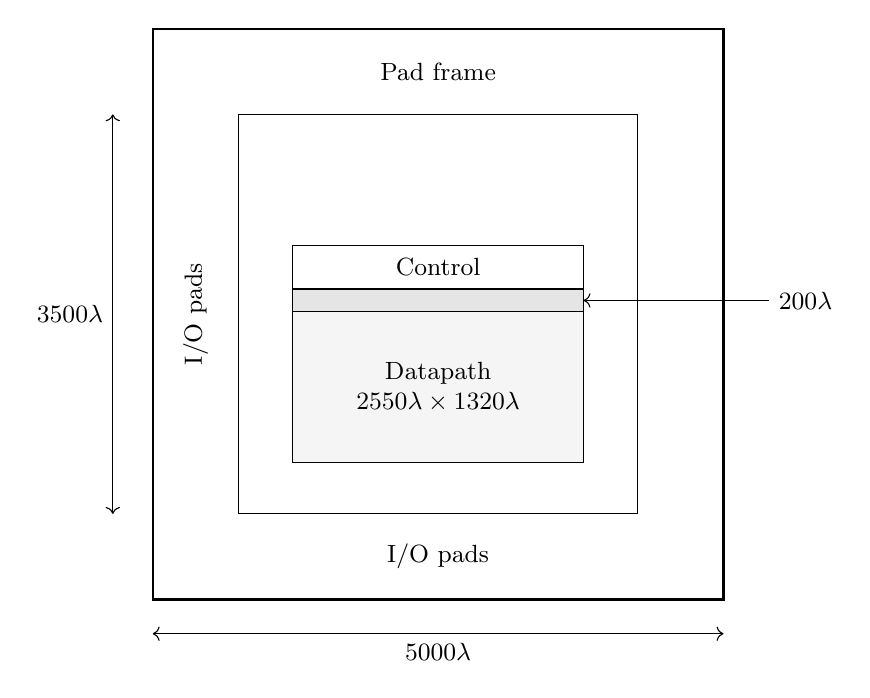
\begin{tikzpicture}[x=0.00145cm,y=0.00145cm,font=\small]
\draw[thick] (0,0) rectangle (5000,5000);
\draw (750,750) rectangle (4250,4250);
\node at (2500,4625) {Pad frame};
\node[rotate=90] at (375,2500) {I/O pads};
\node at (2500,375) {I/O pads};
\draw[fill=gray!8] (1225,1200) rectangle (3775,2520);
\node[align=center] at (2500,1860) {Datapath\\$2550\lambda\times1320\lambda$};
\draw[fill=gray!20] (1225,2520) rectangle (3775,2720);
\draw (1225,2720) rectangle (3775,3100);
\node at (2500,2910) {Control};
\draw[<-] (3775,2620)--(5400,2620) node[right] {$200\lambda$};
\draw[<->] (0,-300)--(5000,-300) node[midway,below] {$5000\lambda$};
\draw[<->] (-350,750)--(-350,4250) node[midway,left] {$3500\lambda$};
\end{tikzpicture}
\end{latin}
\caption{\lr{Floorplan} آموزشی با نسبت ابعاد اصلی کتاب. مستطیل میانی، فضای قابل‌استفاده
داخل \lr{Pad Frame} است. نوار خاکستری کانال کنترل را نشان می‌دهد. جزئیات تک‌تک \lr{Pad}ها حذف شده‌اند
\cite[شکل \secnum{۱.۶۲}]{weste}.}
\label{fig:impl-floorplan}
\end{figure}

\subsection{تبدیل طول و مساحت در مثال کتاب}
در فناوری آموزشی \qty{0.6}{\micro\metre} این مثال، \(\lambda=\qty{0.3}{\micro\metre}\)
است. بنابراین ضلع \(5000\lambda\) برابر \qty{1500}{\micro\metre} یا
\qty{1.5}{\milli\metre} می‌شود. رابطه عمومی تبدیل مساحت چنین است
\begin{equation}
 A_{\mathrm{physical}}=A_{\lambda}\lambda^2.
 \label{eq:impl-area-conversion}
\end{equation}
در این رابطه \(A_{\lambda}\) مقدار عددی مساحت در واحد \(\lambda^2\) است.
چون هر دو بعد طول در \(\lambda\) ضرب می‌شوند، ضریب تبدیل مساحت مربع می‌شود.
در این فناوری، \(1\lambda^2=\qty{0.09}{\micro\metre\squared}\) است.

ابعاد هر \lr{Pad} در کتاب \(750\lambda\times350\lambda\) ذکر شده‌اند.
با کنارگذاشتن حاشیه شعاعی \(750\lambda\) در هر طرف، ضلع فضای داخلی
\(5000-2(750)=3500\lambda\) می‌شود. پس
\begin{align}
 A_{\mathrm{die}}&=(5000\lambda)^2
 =25\times10^6\lambda^2=\qty{2.25}{\milli\metre\squared},\notag\\
 A_{\mathrm{inside}}&=(3500\lambda)^2
 =12.25\times10^6\lambda^2=\qty{1.1025}{\milli\metre\squared}.
 \label{eq:impl-die-core}
\end{align}
مساحت داخل قاب، ظرفیت هندسی موجود را بیان می‌کند. ابعاد بسته پردازنده، شامل دو
بلوک و کانال میان آن‌ها، کوچک‌تر است. با ابعاد گرد‌شده \lr{Floorplan} داریم
\begin{align}
 H_{\mathrm{core}}&=(1320+200+380)\lambda=1900\lambda,\notag\\
 A_{\mathrm{core}}&=(2550)(1900)\lambda^2
 =4.845\times10^6\lambda^2\approx4.8\times10^6\lambda^2.
 \label{eq:impl-core-area}
\end{align}
سهم \lr{Datapath}، کنترل و کانال به‌ترتیب
\(3.366\times10^6\lambda^2\)، \(0.969\times10^6\lambda^2\) و
\(0.510\times10^6\lambda^2\) است. جمع آن‌ها دقیقاً مقدار
\eqref{eq:impl-core-area} را می‌دهد. مقدار فیزیکی متناظر \qty{0.43605}{\milli\metre\squared}
است که برای گزارش تقریبی می‌توان \qty{0.44}{\milli\metre\squared} نوشت.

در این مثال، فضای موردنیاز \lr{Pad Frame} اندازه \lr{Die} را تعیین می‌کند و طراحی
\lr{Pad-limited} است. در طراحی \lr{Core-limited}، اندازه منطق داخلی عامل تعیین‌کننده
مساحت است. کاهش یک بلوک داخلی در حالت اول، تا زمانی که نیاز قاب ثابت بماند،
الزاماً اندازه نهایی \lr{Die} را کاهش نمی‌دهد \cite[صفحه ۴۷]{weste}.

\subsection{گونه‌های ساختار و \lr{Standard Cell}}
کتاب ساختارهای روی تراشه را در گروه‌های \lr{Random Logic}، \lr{Datapath}،
\lr{Array}، \lr{Analog} و \lr{I/O} توضیح می‌دهد \cite[صفحه ۴۸]{weste}.
\lr{Random Logic} اتصال‌های کم‌نظم، مانند \lr{Decoder} منطقی عمومی، دارد.
در \lr{Datapath}، کار مشابه در چند بیت تکرار می‌شود. در \lr{Array}، سلول‌های مشابه
در دو بعد تکرار می‌شوند، مانند \lr{RAM}، \lr{ROM} و \lr{PLA}.
مدار \lr{Analog} و سلول \lr{I/O} به نیازهای الکتریکی و فناوری ویژه خود وابسته‌اند.
تکرار سلولِ طراحی و بررسی‌شده، هزینه طراحی آرایه‌ها را میان نمونه‌های متعدد تقسیم می‌کند.

\lr{Standard Cell} یک سلول کتابخانه‌ای با تابع و هندسه ازپیش‌تعریف‌شده، مانند
\lr{Inverter}، \lr{NAND} یا \lr{Flip-flop}، است. در نمونه کتاب، ریل‌های افقی
تغذیه در \lr{Metal1} عرض \(8\lambda\) و فاصله مرکز تا مرکز \(90\lambda\) دارند.
\lr{nMOS}ها در ناحیه پایین \(40\lambda\) و \lr{pMOS}ها در ناحیه بالای
\(50\lambda\) قرار می‌گیرند. هم‌ترازی ریل و \lr{n-well} امکان اتصال سلول‌های مجاور
از طریق \lr{Abutment} را فراهم می‌کند.

عرض سلول مضربی از \(8\lambda\) است تا تعداد صحیحی مسیر عمودی \lr{Metal2}
داشته باشد. ورودی و خروجی در \lr{Metal2} در دسترس‌اند. \lr{Poly} عمدتاً عمودی و
\lr{Diffusion} و \lr{Metal1} عمدتاً افقی‌اند. اتصال‌های \lr{Substrate} و
\lr{Well} زیر ریل‌ها جا می‌گیرند. فاصله تکرار ردیف‌ها حداقل \(110\lambda\) است.
این اعداد، قواعد کتابخانه آموزشی همان مثال هستند \cite[بخش \secnum{۱.۱۰.۲}]{weste}.

در فرآیند دوفلزی، مسیرهای افقی میان ردیف‌ها به کانال نیاز دارند و تعداد سیم‌ها
ارتفاع کانال را تعیین می‌کند. در مثال سه‌فلزی، \lr{Metal3} افقی با
\lr{Pitch} برابر \(10\lambda\)، روی ارتفاع \(110\lambda\) حدود ۱۱ مسیر فراهم می‌کند.
اگر تقاضای سیم‌کشی در این ظرفیت جا بگیرد، کانال جداگانه می‌تواند حذف شود.
در مثال \lr{MIPS}، جهت‌های غالب \lr{Metal1}، \lr{Metal2} و \lr{Metal3}
به‌ترتیب افقی، عمودی و افقی‌اند. این ترتیب عبور سیم‌ها در لایه‌های مختلف را آسان می‌کند.

کتاب در شکل‌های \secnum{۱.۶۴} و \secnum{۱.۶۵}، نتیجه \lr{Place and Route}
کنترل‌کننده و پردازنده را نشان می‌دهد. نمونه پردازنده در فناوری \qty{130}{\nano\metre}
با هفت لایه فلز، ۲۶ ردیف سلول و حدود \(4\times10^6\lambda^2\) مساحت دارد.
مقایسه تلاش طراحی و سرعت در متن کتاب مربوط به همین زمینه تاریخی است.

\subsection{\lr{Pitch Matching} و \lr{Slice Plan}}
\lr{Pitch} فاصله تکرار یک ساختار است. برای سلول‌هایی که در امتداد یک لبه به هم
می‌چسبند، اندازه و محل اتصال‌های آن لبه باید هماهنگ شوند. این هماهنگی
\lr{Pitch Matching} نام دارد. کوچک‌کردن یک سلول هنگامی که ابعاد نهایی را سلول
همسایه تعیین می‌کند، ممکن است تنها فضای خالی ایجاد کند. بزرگ‌کردن همان سلول نیز
می‌تواند ابعاد همسایه و کل آرایه را افزایش دهد \cite[شکل \secnum{۱.۶۶}]{weste}.

برای نمونه فرضی، چهار سلول با عرض \(w_A\) کنار هم به بلوکی با عرض \(w_B\)
متصل می‌شوند. اگر لبه‌های بیرونی باید هم‌تراز بمانند، عرض موردنیاز ناحیه
\(W=\max(4w_A,w_B)\) است. با \(w_A=20\lambda\) و \(w_B=90\lambda\)،
عرض \(90\lambda\) می‌شود. کاهش \(w_A\) به \(18\lambda\) همچنان همان عرض
نهایی را می‌دهد. برای استفاده از فضای آزاد باید سازمان‌دهی ناحیه نیز بازنگری شود.

\lr{Slice Plan} ترتیب \lr{Wordslice}ها و تخصیص مسیرها در هر \lr{Bitslice} را
پیش از رسم جزئیات مشخص می‌کند. در شکل \secnum{۱.۶۸} کتاب، نقطه روی مسیر بیان می‌کند
که گذرگاه علاوه بر عبور از سلول، در آن سلول مصرف یا تولید می‌شود. پهنای هر جزء با
تعداد مسیر نوشته شده است. بیشترین تراکم این مثال روی \lr{Register File} و برابر
هفت مسیر است \cite[بخش \secnum{۱.۱۰.۴}]{weste}.

جمع عرض اجزای شکل کتاب ۳۱۹ مسیر است. با \lr{Pitch} برابر \(8\lambda\)،
عرض \lr{Datapath} چنین محاسبه می‌شود
\begin{equation}
 W_{\mathrm{data}}=319\times8\lambda=2552\lambda.
 \label{eq:impl-slice-width}
\end{equation}
عدد \(2550\lambda\) در \lr{Floorplan}، مقدار گرد‌شده همین تخمین است.
ارتفاع از هشت \lr{Bitslice}، یک ردیف \lr{Zipper} و سه ردیف \lr{Address Decoder}
ساخته می‌شود. پس با ۱۲ ردیف و فاصله \(110\lambda\)، ارتفاع
\(12(110)\lambda=1320\lambda\) است. فضای خالی ردیف‌های \lr{Decoder} در طراحی
فشرده‌تر می‌تواند برای بخش دیگری مانند کنترل استفاده شود. این تغییر به سازگاری
اتصال و زمان‌بندی نیاز دارد.

\subsection{\lr{Array} و نمونه \lr{PLA}}
\lr{Programmable Logic Array} یا \lr{PLA} توابع به صورت \lr{Sum of Products}
را با دو صفحه پیاده می‌کند. \lr{AND Plane} جمله‌های حاصل‌ضرب و \lr{OR Plane}
ترکیب آن‌ها را می‌سازد. برای نمونه، \(F=ab+ac\) به دو جمله حاصل‌ضرب و یک خروجی
نیاز دارد. در کنترل‌کننده کتاب، این ساختار منطق حالت بعد و خروجی \lr{FSM} را
پیاده می‌کند \cite[بخش \secnum{۱.۱۰.۵}، شکل \secnum{۱.۶۹}]{weste}.

برای قالب آموزشی همان کتاب، هر ورودی دو مسیر عمودی، هر خروجی سه مسیر عمودی و
حاشیه حدود شش مسیر می‌خواهد. هر جمله حاصل‌ضرب حدود یک‌ونیم مسیر افقی و حاشیه
حدود ۱۴ مسیر لازم دارد. اگر \(n_i,n_o,n_p\) به‌ترتیب تعداد ورودی، خروجی و جمله
حاصل‌ضرب و \(p_v,p_h\) فاصله مسیرهای عمودی و افقی باشند، تخمین ساختاری برابر است با
\begin{equation}
 W\approx(2n_i+3n_o+6)p_v,\qquad
 H\approx(1.5n_p+14)p_h.
 \label{eq:impl-pla-estimate}
\end{equation}
فاصله مسیر هر جهت باید از همان قالب سلول تعیین شود. این رابطه رشد عرض با ورودی
و خروجی و رشد ارتفاع با تعداد جمله‌ها را روشن می‌کند.

\lr{PLA} مثال کتاب \(500\lambda\times350\lambda\) است و چهار \lr{Flip-flop}
خارجی ناحیه \(336\lambda\times220\lambda\) دارند. جمع مساحت این دو بخش
\(175000+73920=248920\lambda^2\) می‌شود. مساحت کنترل‌کننده باید سیم‌های ورودی
و خروجی و الزامات جانمایی را نیز در بر بگیرد. برای مقایسه، نمونه کنترل‌کننده حاصل
از ابزار در شکل \secnum{۱.۶۴} ابعاد \(1500\lambda\times400\lambda\) دارد و
بخش بزرگی از آن را کانال‌ها اشغال می‌کنند. این دو سازمان‌دهی و \lr{Floorplan}
بالادستی را با ابعاد و قیود مخصوص خود مقایسه می‌کنیم.

\subsection{تخمین مساحت و دقت اعداد}
تخمین زودهنگام می‌تواند از بلوک مشابه پیشین یا از چگالی تقریبی آغاز شود.
جدول \ref{tab:impl-density} داده‌های جدول \secnum{۱.۱۰} کتاب را با واحد روشن
بازنویسی می‌کند. این اعداد به فناوری، قالب سلول و روش سیم‌کشی وابسته‌اند.
\begin{table}[ht]
\centering
\caption{چگالی‌های تقریبی آموزشی کتاب برای تخمین اولیه \cite[صفحه ۵۲]{weste}.}
\label{tab:impl-density}
\begin{tabularx}{\textwidth}{rX}
\toprule
ساختار & مساحت تقریبی\\
\midrule
\lr{Random Logic} با دو لایه فلز & \(1000\) تا \(1500\lambda^2\) به‌ازای ترانزیستور\\
\lr{Datapath} & \(250\) تا \(750\lambda^2\) به‌ازای ترانزیستور، یا مدل \(6WL+360\lambda^2\)\\
\lr{SRAM} & \(1000\lambda^2\) به‌ازای بیت\\
\lr{DRAM} در فرآیند ویژه آن & \(100\lambda^2\) به‌ازای بیت\\
\lr{ROM} & \(100\lambda^2\) به‌ازای بیت\\
\bottomrule
\end{tabularx}
\end{table}
در مدل \(6WL+360\lambda^2\)، طول‌های \(W,L\) باید با واحد طول سازگار جای‌گذاری
شوند تا \(WL\) مساحت شود. برای حافظه، مساحت بیت‌ها به همراه \lr{Decoder} و مدارهای
جانبی در نظر گرفته می‌شود. تخمین کانال نیز از تعداد مسیر ضرب‌در \lr{Pitch}
آغاز می‌شود. کاهش جزئی سلولی که بارها تکرار می‌شود می‌تواند در سطح کل تراشه اثر
زیادی بگذارد. تخمین محافظه‌کارانه، فضای لازم برای اصلاح و رشد بلوک را فراهم می‌کند.

گاهی چگالی به صورت \lr{kgates/mm²} گزارش می‌شود. کتاب در مثال خود، هر \lr{Gate}
معادل را یک \lr{NAND3} یا \lr{NOR3} شش‌ترانزیستوری می‌گیرد. با این تعریف و
\(\lambda\approx\qty{0.03}{\micro\metre}\)، چگالی
\(160\) تا \(500\) هزار \lr{Gate} در \unit{\milli\metre\squared} به‌ترتیب حدود
\(1160\) تا \(370\lambda^2\) برای هر ترانزیستور می‌دهد
\cite[صفحه ۵۳]{weste}. برای مقدار ۱۶۰ هزار، محاسبه چنین است
\begin{equation}
 a_{\mathrm{tr}}\approx
 \frac{10^6\,\unit{\micro\metre\squared}}
 {160000\times6}\,
 \frac{\lambda^2}{0.03^2\,\unit{\micro\metre\squared}}
 \approx1160\lambda^2.
 \label{eq:impl-density-conversion}
\end{equation}
افزایش چگالی، مساحت متناظر هر ترانزیستور را کاهش می‌دهد. مقایسه دو گزارش چگالی
باید با تعریف یکسان \lr{Gate} و محدوده یکسان سیم‌کشی انجام شود.

\clearpage
\subsection{تمرین‌های پاسخ‌دار \lr{Physical Design}}
\textbf{تمرین ۱.} بلوک فرضی با ۱۰ هزار ترانزیستور و تخمین
\(1000\lambda^2\) برای هر ترانزیستور، در فناوری \(\lambda=\qty{0.1}{\micro\metre}\)
چه مساحتی دارد؟ ابتدا مساحت در واحد \(\lambda^2\) برابر \(10^7\lambda^2\) است.
پس مساحت فیزیکی \(10^7(0.1)^2=10^5\,\unit{\micro\metre\squared}\) یا
\qty{0.1}{\milli\metre\squared} می‌شود. برای فرض مربع‌بودن بلوک، ضلع
\(\sqrt{0.1}\,\unit{\milli\metre}\approx\qty{0.316}{\milli\metre}\) است.
این تخمین باید با محدوده‌ای که چگالی گزارش‌شده پوشش می‌دهد تفسیر شود.

\textbf{تمرین ۲.} برای کانال فرضی ۲۵ مسیر با فاصله \(8\lambda\)، ارتفاع لازم
در مدل کتاب چقدر است؟ حاصل \(25(8)\lambda=200\lambda\) می‌شود.
در \(\lambda=\qty{0.3}{\micro\metre}\)، ارتفاع \qty{60}{\micro\metre} است.
عرض کانال \(2550\lambda\) باشد، مساحت \(510000\lambda^2\) یا
\qty{45900}{\micro\metre\squared} خواهد بود.

\textbf{تمرین ۳.} اگر عرض \lr{Datapath} از ۳۱۹ به ۳۰۰ مسیر برسد و ارتفاع
۱۲ ردیفی ثابت بماند، کاهش مساحت چقدر است؟ عرض جدید \(2400\lambda\) و کاهش
عرض \((319-300)8\lambda=152\lambda\) است. کاهش مساحت برابر
\(152(1320)\lambda^2=200640\lambda^2\)، یعنی حدود ۶ درصد مساحت اولیه
\(2552(1320)\lambda^2\)، می‌شود. تغییر مساحت کل \lr{Die} به عامل تعیین‌کننده
ابعاد نهایی نیز وابسته است.
\clearpage

\section{بررسی درستی طراحی}
\label{sec:book-verification}
\subsection{رابطه میان \lr{Specification} و نمایش‌های طراحی}
\lr{Verification} بررسی می‌کند که طراحی با رفتار و محدودیت‌های مورد انتظار
سازگار باشد. \lr{Specification} باید رفتار خروجی، شرایط ورودی، \lr{Reset}،
زمان‌بندی و سایر قیود لازم را مشخص کند. با دقیق‌ترشدن نمایش، تعداد جزئیات و هزینه
تحلیل افزایش می‌یابد. کتاب برای مدیریت این هزینه، بررسی عملکرد در سطوح بالاتر و
بررسی سازگاری میان نمایش‌های متوالی را توضیح می‌دهد
\cite[بخش \secnum{۱.۱۱}، شکل \secnum{۱.۷۰}]{weste}.

در سطح معماری، مدل رفتاری مانند برنامه \lr{C} با تعریف معماری سنجیده می‌شود.
در سطح منطق، \lr{HDL} با ورودی و خروجی مورد انتظار بررسی می‌شود. در مرحله مدار،
عملکرد شبکه ترانزیستور با تابع منطقی مقایسه می‌شود. در مرحله فیزیکی، اتصال‌های
استخراج‌شده از \lr{Layout} با \lr{Schematic} مقایسه می‌شوند. در کنار این زنجیره،
مدار و \lr{Layout} باید قیود زمان‌بندی و توان را برآورده کنند.

برای نمونه، اگر نیاز سیستم جمع هشت‌بیتی با \lr{Carry-out} باشد، رفتار مرجع باید
جمع کامل ۹ بیتی را مشخص کند. سپس خروجی هشت‌بیتی، هشت بیت کم‌ارزش نتیجه و
\lr{Carry-out} بیت نهم است. اگر تعریف علامت‌دار بودن داده یا رفتار \lr{Overflow}
مبهم بماند، پاسخ مورد انتظار آزمون نیز مبهم می‌شود.

\subsection{\lr{Testbench} و انتخاب ورودی‌ها}
\lr{Testbench} محیطی است که \lr{Device Under Test} یا \lr{DUT} را نمونه‌سازی
می‌کند، ورودی‌ها را اعمال می‌کند و پاسخ را با مرجع مقایسه می‌کند. یک \lr{Test Vector}
می‌تواند شامل ورودی و پاسخ مورد انتظار باشد. در مدار ترتیبی، زمان اعمال ورودی،
\lr{Clock}، \lr{Reset} و وضعیت قبلی نیز بخشی از سناریو هستند
\cite[صفحه ۵۳]{weste}.

برای تابع ترکیبی با \(n\) ورودی دودویی، تعداد حالت‌ها \(2^n\) است، زیرا برای هر
ورودی دو انتخاب مستقل داریم. \lr{Carry} سه‌ورودی ۸ حالت دارد. جمع‌کننده هشت‌بیتی
با دو عملوند هشت‌بیتی و یک \lr{Carry-in}، تعداد
\(2^{8+8+1}=131072\) حالت دارد. با افزایش ورودی‌ها، بررسی کامل به‌سرعت پرهزینه
می‌شود. برای مدار ترتیبی، ترتیب ورودی‌ها و حالت داخلی نیز باید بررسی شوند.

در نمونه آموزشی، برای جمع‌کننده ورودی‌های صفر، بیشینه مقدار، تولید و انتشار
\lr{Carry} و الگوهای مکمل ارزش بررسی دارند. در پردازنده، \lr{Reset}، هر نوع دستور،
شاخه گرفته‌شده و گرفته‌نشده و مرز نشانی‌ها باید طبق تعریف معماری آزموده شوند.
پاسخ مرجع باید از صورت مسئله و محاسبه مستقل به دست آید. کپی همان عبارت اشتباه
از طراحی به مرجع می‌تواند همان خطا را در هر دو حفظ کند.

\lr{Post-synthesis Netlist} را می‌توان با بردارهای آزمون قبلی شبیه‌سازی کرد.
برای شبکه ترانزیستور نیز آزمون عملکرد ممکن است. در مدار ترتیبی، ترتیب رخدادها و
\lr{Race Condition} اهمیت پیدا می‌کند. ابزار \lr{Formal Verification} نیز می‌تواند
تحت فرض‌ها و مدل تعریف‌شده، هم‌ارزی تابع یا خاصیت را بررسی کند.
کیفیت فرض‌ها و پوشش حالت‌ها بر معنای نتیجه اثر می‌گذارد.

\subsection{\lr{DRC}، \lr{LVS}، \lr{ERC} و تحلیل الکتریکی}
\lr{Design Rule Check} یا \lr{DRC} هندسه را با قواعد فناوری مقایسه می‌کند، مانند
حداقل عرض، فاصله و پوشش اتصال. \lr{Layout Versus Schematic} یا \lr{LVS} بررسی
می‌کند که ترانزیستورها و اتصال‌های استخراج‌شده از \lr{Layout} با مدار مرجع سازگار
باشند. \lr{Electrical Rule Check} یا \lr{ERC} برای یافتن مسئله‌های الکتریکی
تعریف‌شده در مجموعه قواعد به کار می‌رود. کتاب به مشکلاتی مانند نویز یا فرسودگی
زودهنگام اشاره می‌کند \cite[صفحه ۵۳]{weste}.

جدول \ref{tab:impl-verification} مثال‌هایی از ارتباط خطا و بررسی مناسب را نشان می‌دهد.
یک مسئله ممکن است در بیش از یک بررسی آشکار شود و توان کشف هر ابزار به مدل و قواعدش وابسته است.
\begin{table}[ht]
\centering
\caption{نمونه ارتباط مسئله طراحی با بررسی لازم.}
\label{tab:impl-verification}
\begin{tabularx}{\textwidth}{rX}
\toprule
مسئله & بررسی مرتبط\\
\midrule
اشتباه در تابع \lr{Carry} & مقایسه رفتاری، جدول کامل یا بررسی هم‌ارزی\\
سیم با عرض کمتر از حد مجاز & \lr{DRC} با قواعد فناوری\\
اتصال خروجی به گره داخلی اشتباه & \lr{LVS} در برابر مدار مرجع\\
اتصال الکتریکی نامناسب تغذیه یا \lr{Body} & \lr{ERC} و بررسی اتصال با قواعد مرتبط\\
رسیدن خروجی پس از مهلت لازم & تحلیل زمان‌بندی با مدل مناسب مدار و سیم\\
مصرف توان بیشتر از بودجه & تحلیل توان با تحریک، فعالیت و مدل معتبر\\
\bottomrule
\end{tabularx}
\end{table}

اگر هندسه قانونی باشد اما دو گره منطقی جابه‌جا شده باشند، ممکن است
\lr{DRC} بدون خطای هندسی پایان یابد و \lr{LVS} اختلاف اتصال را پیدا کند.
اگر اتصال با مرجع برابر باشد اما خود مرجع تابع اشتباه داشته باشد، مقایسه رفتاری
با \lr{Specification} لازم است. برای بررسی سرعت و توان نیز مقاومت و خازن سیم،
اندازه ترانزیستور، ولتاژ و شرایط مدل‌شده اهمیت دارند.

\subsection{تمرین‌های پاسخ‌دار \lr{Verification}}
\textbf{تمرین ۱.} در گیت \lr{NAND2}، خروجی در \lr{Layout} به \(V_{DD}\) اتصال
پیدا کرده است. آزمون عملکرد چه ورودی‌ای را باید حتماً اعمال کند؟
برای \(a=b=1\)، پاسخ مرجع صفر است. خروجی ثابت یک اختلاف را آشکار می‌کند.
سه حالت دیگر خروجی مرجع یک دارند و این خطا را در مدل خروجی ثابت نشان نمی‌دهند.
\lr{LVS} نیز باید اختلاف اتصال با مدار صحیح را بررسی کند.

\textbf{تمرین ۲.} مدار تابع درست را با تأخیر \qty{2}{\nano\second} تولید می‌کند،
ولی مهلت داده‌شده \qty{1.5}{\nano\second} است. نتیجه چیست؟
شرط عملکرد منطقی برآورده شده، اما قید زمان‌بندی \qty{0.5}{\nano\second} نقض شده است.
برای اعلام موفقیت باید هر دو شرط تابع و مهلت برقرار باشند.

\textbf{تمرین ۳.} آیا یک آزمون موفق برنامه \lr{Fibonacci}، همه حالت‌های پردازنده
را پوشش می‌دهد؟ این برنامه تنها توالی مشخصی از دستورها، داده‌ها و شاخه‌ها را طی
می‌کند. برای پوشش نیازهای دیگر باید سناریوهای متناسب با همان نیازها افزوده شود.
مثلاً صحت \lr{Reset}، دستور استفاده‌نشده و حالت مرزی \lr{Branch} به بررسی مربوط خود نیاز دارد.
\clearpage

\section{ساخت، \lr{Packaging} و \lr{Testing}}
\label{sec:book-manufacturing}
\subsection{\lr{Tapeout}، \lr{Mask} و تقسیم هزینه ساخت}
پس از نهایی‌شدن طراحی و بررسی‌های لازم، توصیف هندسه ماسک‌ها برای ساخت تحویل
داده می‌شود. این مرحله \lr{Tapeout} نام دارد. نام آن از روش تاریخی تحویل داده روی
نوار مغناطیسی آمده است. کتاب قالب‌های \lr{Caltech Interchange Format} یا
\lr{CIF} و \lr{Calma GDS II Stream Format} یا \lr{GDS} را معرفی می‌کند
\cite[بخش \secnum{۱.۱۲}]{weste}.

\lr{Mask} الگوی لازم برای انتقال هندسه یک مرحله از فرآیند را فراهم می‌کند.
کتاب روش ساخت الگوی کروم روی شیشه با پرتو الکترونی را توضیح می‌دهد.
هزینه ماسک و تجهیز خط تولید، بخش مهمی از هزینه ثابت ساخت است.
متن سال ۲۰۱۱ برای مثال‌های \qty{180}{\nano\metre} و \qty{65}{\nano\metre}
به‌ترتیب حدود ۲۵۰ هزار و ۳ میلیون دلار هزینه مجموعه ماسک ذکر می‌کند.
این مقادیر، مثال تاریخی همان کتاب‌اند.

در \lr{Multi-project Wafer}، چند طراحی کوچک از مجموعه مشترکی از ماسک‌ها استفاده
می‌کنند تا هزینه ثابت میان مشتریان تقسیم شود. کتاب خدمات \lr{MOSIS}،
\lr{EUROPRACTICE} و \lr{VDEC} را در زمینه زمان انتشار معرفی می‌کند.
در مدل آموزشی فرضی، اگر هزینه ثابت مشترک \(K\) میان \(N\) طراحی با سهم برابر
تقسیم شود، سهم هر طراحی \(K/N\) است. هزینه عملی به سهم سطح، فرآیند، تعداد نمونه،
\lr{Packaging} و شرایط خدمات وابسته است.

\lr{Fab} کارخانه ساخت و \lr{Foundry} تأمین‌کننده خدمات ساخت است.
شرکت \lr{Fabless} طراحی را انجام می‌دهد و ساخت را به کارخانه طرف قرارداد می‌سپارد.
کتاب هزینه بالای تأسیس کارخانه و اهمیت اقتصادی این تقسیم کار را توضیح می‌دهد.

\subsection{از \lr{Wafer} تا \lr{Die}}
روی یک \lr{Wafer} سیلیکونی، تعداد زیادی نسخه مدار هم‌زمان ساخته می‌شوند.
مراحل تکراری رسوب‌دهی، ماسک‌گذاری، \lr{Etch} و \lr{Implant} همان هندسه و
ساختار افزاره را ایجاد می‌کنند که در بخش ساخت مقدماتی آموختیم.
کتاب قطرهای \qty{150}{\milli\metre} تا \qty{300}{\milli\metre} و زمان بازگشت
تا حدود ۱۰ هفته را برای زمینه صنعتی زمان خود شرح می‌دهد \cite[صفحه ۵۴]{weste}.

در \lr{Clean Room}، فیلتر هوا و پوشش کارکنان، ورود ذرات آلاینده را کاهش می‌دهد.
یک ذره کوچک می‌تواند بخشی از الگو را خراب کند و اتصال باز یا اتصال کوتاه بسازد.
پس از فرآوری، \lr{Wafer} به قطعه‌های \lr{Die} بریده می‌شود. هندسه نهایی قطعه،
تعداد و محل اتصال‌ها و نیاز حرارتی، در انتخاب \lr{Package} نقش دارند.

\subsection{\lr{Wire Bonding} و \lr{Flip-chip}}
\lr{Package} اتصال قابل‌استفاده با محیط بیرونی و حفاظت مکانیکی قطعه را فراهم
می‌کند و در دفع گرما و رفتار الکتریکی نیز نقش دارد. مثال \lr{MIPS} کتاب، قطعه
\qty{1.5}{\milli\metre} در \qty{1.5}{\milli\metre} را در \lr{Dual-inline Package}
یا \lr{DIP} با ۴۰ پایه نشان می‌دهد. در \lr{Wire Bonding}، سیم‌های نازک طلا
\lr{Pad}های قطعه را به \lr{Lead Frame} بسته وصل می‌کنند
\cite[شکل \secnum{۱.۷۳} و صفحه ۵۵]{weste}.

در \lr{Flip-chip}، اتصال‌های لحیمی کوچک روی سطح قطعه ایجاد می‌شوند و قطعه
روبه‌پایین به زیرلایه متصل می‌شود. امکان توزیع اتصال‌ها در سطح تراشه، ظرفیت اتصال
را افزایش می‌دهد. حذف سیم \lr{Bond Wire} سهم القایی آن سیم را از مسیر برمی‌دارد.
رفتار الکتریکی نهایی همچنان به کل مسیر اتصال و بسته وابسته است.
کتاب معیارهای هزینه، تعداد پایه، پهنای باند پایه، انتقال توان و قابلیت اطمینان را
برای مقایسه بسته‌ها مطرح می‌کند و جزئیات را به فصل ۱۳ ارجاع می‌دهد.

\subsection{آزمون قطعه ساخته‌شده و \lr{BIST}}
\lr{Testing} قطعه ساخته‌شده را با معیار پذیرش می‌سنجد تا نمونه‌های دارای عیب
شناسایی شوند. حتی با طراحی صحیح، نقص ساخت یا آلودگی می‌تواند قطعه معیوب ایجاد کند.
آزمون به دسترسی ورودی‌ها، مشاهده پاسخ‌ها، سرعت موردنظر و هزینه زمانی دستگاه
آزمون وابسته است \cite[صفحه ۵۵]{weste}.

در \lr{Built-in Self-test} یا \lr{BIST}، مدارهای کمکی روی تراشه بخشی از تولید
تحریک و بررسی پاسخ را انجام می‌دهند. هدف معرفی‌شده در کتاب کاهش زمان لازم
دستگاه آزمون خارجی است. این انتخاب، منطق و مساحت کمکی می‌خواهد.
پوشش عیب به روش تولید الگو و تحلیل پاسخ وابسته است.
معیار آزمون باید با عیب‌هایی که قصد کشفشان را داریم متناسب باشد.

برای تحلیل اقتصادی ساده، \lr{Yield} را نسبت تعداد قطعات سالم به تعداد قطعات
ساخته‌شده تعریف می‌کنیم. اگر به فرض ۱۰۰۰ قطعه ساخته شود و ۸۵۰ قطعه معیار پذیرش
را برآورده کنند، \(Y=850/1000=0.85\)، یعنی ۸۵ درصد است.
اگر هزینه مفروض همین مرحله \(K\) باشد، هزینه سرشکن‌شده هر قطعه سالم در این مدل
\begin{equation}
 C_{\mathrm{good}}=\frac{K}{N_{\mathrm{good}}}
 =\frac{K}{YN_{\mathrm{total}}}
 \label{eq:impl-yield-cost}
\end{equation}
خواهد بود. \(N_{\mathrm{total}}\) تعداد کل و \(N_{\mathrm{good}}\) تعداد سالم است.
با ثابت‌بودن هزینه و تعداد ساخت، کاهش \lr{Yield} هزینه هر قطعه سالم را افزایش می‌دهد.
این مثال افزوده، مدل سرشکن‌کردن یک هزینه مشخص است. هزینه‌های مراحل دیگر باید
در مدل اقتصادی کامل خود لحاظ شوند.

\subsection{تمرین‌های پاسخ‌دار ساخت و آزمون}
\textbf{تمرین ۱.} هزینه فرضی یک مرحله برای ۱۰۰۰ قطعه، ۲۰ هزار واحد پول است.
با \lr{Yield} برابر ۸۰ درصد، هزینه همان مرحله برای هر قطعه سالم چقدر می‌شود؟
تعداد سالم \(0.8(1000)=800\) و هزینه واحد \(20000/800=25\) واحد پول است.
با \lr{Yield} برابر ۵۰ درصد، هزینه \(20000/500=40\) واحد پول می‌شود.

\textbf{تمرین ۲.} برای عیب خروجی گیرکرده روی صفر در \lr{Carry}، چه ورودی‌ای مناسب است؟
مثلاً \(a=b=1,c=0\) پاسخ مرجع یک دارد و عیب را در مدل گیرکردن خروجی آشکار می‌کند.
ورودی \(0,0,0\) پاسخ مرجع صفر دارد و این عیب خاص را آشکار نمی‌کند.
همان منطق انتخاب تحریک در \lr{Testbench} نیز کاربرد دارد.

\textbf{تمرین ۳.} اگر \lr{LVS} و آزمون عملکرد پیش از ساخت موفق باشند، قطعه ساخته‌شده
چه بررسی دیگری می‌خواهد؟ شرایط ساخت هر نمونه می‌تواند نقص ایجاد کند، بنابراین
آزمون قطعه با معیارهای عملکرد و کیفیت تعیین‌شده لازم است. صحت اتصال استخراج‌شده،
صحت رفتار مدل و سلامت نمونه فیزیکی، هر یک به شواهد مناسب خود وابسته‌اند.

\subsection{پیوند این بخش با مدل‌های فصل ۲}
برای محاسبه دقیق‌تر تأخیر باید بدانیم جریان ترانزیستور چگونه به
\(V_{GS}\)، \(V_{DS}\)، \(V_{BS}\)، \(W\) و \(L\) وابسته است.
برای محاسبه بار باید خازن‌های \lr{Gate}، \lr{Diffusion} و سیم را بشناسیم.
برای ارزیابی حالت منطقی پایدار نیز رابطه ورودی و خروجی \lr{Inverter} اهمیت دارد.
بخش‌های آغازین فصل ۲ این مدل‌های افزاره را می‌سازند و بخش‌های بعدی اثرهای غیرایده‌آل
و مشخصه‌های \lr{DC} را به آن‌ها اضافه می‌کنند.
\clearpage

\section*{جمع‌بندی اهداف طراحی و هزینه}
\phantomsection
\addcontentsline{toc}{section}{جمع‌بندی اهداف طراحی و هزینه}
\label{sec:book-objectives}
جمع‌بندی فصل ۱ کتاب چهار هدف \lr{Reliability}، \lr{Performance}، \lr{Power}
و \lr{Cost} را کنار هم قرار می‌دهد \cite[صفحات چاپی ۵۵ و ۵۶]{weste}.
\lr{Reliability} به عملکرد قابل‌قبول در شرایط و طول عمر مورد انتظار مربوط است.
ولتاژ و دمای مجاز، بخشی از این شرایط‌اند.
\lr{Performance} به زمان انجام کار و توان عملیاتی وابسته است و با فرکانس
\lr{Clock} و میزان موازی‌سازی ارتباط دارد.
توان، محدودیت حرارتی و مصرف انرژی را به انتخاب مدار و فعالیت آن پیوند می‌دهد.
هزینه نیز از تلاش طراحی، ماسک و تولید هر قطعه اثر می‌پذیرد.

\subsection*{هزینه ثابت و هزینه هر قطعه}
\lr{Nonrecurring Engineering} یا \lr{NRE} هزینه‌هایی مانند طراحی و تهیه ماسک
را دربرمی‌گیرد. برای مدل اقتصادی آموزشی، \(K\) را هزینه ثابت، \(c\) را هزینه
تولید هر قطعه و \(N>0\) را تعداد قطعه می‌نامیم.
با فرض ثابت‌بودن \(c\) و لحاظ‌شدن شرایط تولید در همین ضریب، هزینه کل و میانگین برابرند با
\begin{equation}
 C_{\mathrm{total}}=K+Nc,\qquad
 C_{\mathrm{unit}}=\frac{K}{N}+c.
 \label{eq:booklet-nre}
\end{equation}
با افزایش تعداد تولید، سهم هزینه ثابت در هر قطعه کاهش می‌یابد.
کتاب این سازوکار را در مقایسه فناوری با هزینه مهندسی بالا و فناوری بالغ‌تر
توضیح می‌دهد. هزینه واقعی به مساحت، فرآیند، \lr{Yield}، بسته‌بندی و شرایط تولید
وابسته است. اعداد نمونه این پاراگراف برای تحلیل روش فرض می‌شوند.

دو انتخاب فرضی \(A\) و \(B\) با داده‌های
\(K_A=100000\)، \(c_A=5\)، \(K_B=400000\) و \(c_B=2\)، همگی در واحد پول
سازگار، را در نظر بگیرید.
برای \(N=10000\)، میانگین‌ها \(100000/10000+5=15\) و
\(400000/10000+2=42\) واحد پول‌اند.
برای یافتن تعداد برابری، دو رابطه را برابر می‌کنیم
\begin{equation}
 \frac{100000}{N}+5=\frac{400000}{N}+2
 \quad\Longrightarrow\quad
 3=\frac{300000}{N}
 \quad\Longrightarrow\quad N=100000.
 \label{eq:booklet-cost-crossover}
\end{equation}
در این تعداد، هر دو میانگین ۶ واحد پول می‌شوند.
برای تولید کمتر، \(A\) و برای تولید بیشتر، \(B\) در همین فرض‌ها هزینه میانگین
کمتری دارد. این مثال از مفهوم هزینه ثابت در جمع‌بندی کتاب بسط داده شده است.

\subsection*{پیوند مدل‌های درس با تصمیم طراحی}
انتخاب شبکه منطقی و اندازه ترانزیستور، جریان و ظرفیت را تغییر می‌دهد.
این دو کمیت، زمان شارژ و تخلیه را تعیین می‌کنند.
انتخاب \lr{Layout}، طول سیم، مساحت پیوندها و فضای سیم‌کشی را تغییر می‌دهد.
روش ساخت و بسته‌بندی نیز بر محدودیت الکتریکی، هزینه و قابلیت اطمینان اثر دارند.
برای ارزیابی یک تصمیم، باید فرض عملکرد، معیار زمان، بودجه توان و مدل فیزیکی
مورد استفاده مشخص باشد.
فصل ۲ این جزوه، مدل جریان و ظرفیت لازم برای آغاز این محاسبه را فراهم می‌کند.
\clearpage


\chapter{مدل جریان و ظرفیت ترانزیستور \lr{MOS}}
\label{chap:mos-theory}
در این فصل، بخش‌های \secnum{۲.۱} تا \secnum{۲.۳} کتاب با استخراج روابط و
کنترل شرط‌های اعتبار مطالعه می‌شوند. نمادهای کوچک \(V_{gs},I_{ds}\) در بحث
مقدماتی و نمادهای \(V_{GS},I_{DS}\) در استخراج تفصیلی، به یک کمیت اشاره دارند.
برای \lr{pMOS}، قرارداد بزرگی مثبت و قرارداد علامت‌دار به‌صراحت معرفی می‌شوند.
\section{ساختار و عملکرد فیزیکی \lr{MOS}}
\label{sec:book-mos-structure}
\subsection{\lr{Silicon}، \lr{Dopant} و حامل متحرک}
اتم \lr{Silicon} چهار الکترون ظرفیت دارد و در شبکه بلوری با همسایه‌ها پیوند
تشکیل می‌دهد. هدایت الکتریکی به وجود حامل‌های متحرک وابسته است.
در دمای غیرصفر، \lr{Silicon} خالص نیز می‌تواند الکترون و \lr{Hole} ناشی از
برانگیزش گرمایی داشته باشد. افزودن مقدار کنترل‌شده ناخالصی، یا \lr{Doping}،
تعداد و نوع حامل غالب را تغییر می‌دهد. اسلایدهای ۲ و ۳ این مقدمه را به صورت
تصویر شبکه و ناخالصی نشان می‌دهند \cite{mos}.

در \lr{n-type}، ناخالصی \lr{Donor} از گروه پنج، مانند \lr{Arsenic}، یک الکترون
اضافی در اختیار هدایت می‌گذارد. پس از آزادشدن الکترون، یون ناخالصی مثبت در شبکه
باقی می‌ماند. در \lr{p-type}، ناخالصی \lr{Acceptor} از گروه سه، مانند
\lr{Boron}، کمبود الکترونی ایجاد می‌کند که به صورت \lr{Hole} توصیف می‌شود.
حرکت پی‌درپی الکترون‌های پیوندی برای پرکردن این جای خالی، مانند جابه‌جایی
حاملی با بار مثبت دیده می‌شود. یون‌های ناخالصی در شبکه ثابت‌اند، اما حامل‌ها متحرک‌اند.

در \lr{n-type}، الکترون‌ها و در \lr{p-type}، \lr{Hole}ها حامل غالب‌اند.
\lr{Doping} معمولاً ماده را در مقیاس حجمی تقریباً خنثی نگه می‌دارد، زیرا بار
حامل‌های متحرک و یون‌ها یکدیگر را جبران می‌کنند. در ناحیه \lr{Depletion}،
خارج‌شدن حامل‌های متحرک، بار یون‌های ثابت را آشکار می‌کند.
این توضیح، معنای دقیق‌تر تقریب «نبود حامل آزاد» در مدل مقدماتی اسلاید ۳ و
متن ساده‌شده صفحه ۶۲ کتاب را فراهم می‌کند.

\subsection{پیوند \lr{p-n} و اتصال \lr{Body}}
تماس ناحیه \lr{p-type} و \lr{n-type} یک پیوند \lr{p-n} می‌سازد.
در مدل دیودی، سمت \lr{p}، \lr{Anode} و سمت \lr{n}، \lr{Cathode} است.
وقتی ولتاژ سمت \lr{p} نسبت به سمت \lr{n} افزایش کافی داشته باشد، پیوند
\lr{Forward-biased} می‌شود. با منفی‌ترشدن سمت \lr{p} نسبت به سمت \lr{n}،
پیوند \lr{Reverse-biased} است و جریان نشتی کوچکی دارد. این مدل مقدماتی
در اسلاید ۴ معرفی شده است \cite{mos}.

در \lr{nMOS}، دو ناحیه \(n^+\) داخل \lr{Body} نوع \lr{p} قرار دارند.
هر یک با \lr{Body} پیوند دیودی دارد. با اتصال \lr{Body} به زمین و ولتاژهای
نامنفی \lr{Source} و \lr{Drain}، این پیوندها بایاس صفر یا معکوس دارند.
در \lr{pMOS}، ناحیه‌های \(p^+\) داخل \lr{Body} نوع \lr{n} هستند و معمولاً
\lr{Body} به بالاترین تغذیه وصل می‌شود. این اتصال پیوندها را در شرایط معمول
مدار از هدایت مستقیم دور نگه می‌دارد \cite[صفحات ۶۲ تا ۶۴]{weste}.

علامت \(+\) در \(n^+\) یا \(p^+\) بیانگر شدت بیشتر \lr{Doping} است.
در ساختمان \lr{MOS}، مسیر کنترل‌شده جریان از لایه زیر \lr{Gate} عبور می‌کند.
بایاس ناخواسته پیوند \lr{Body} می‌تواند مسیر دیگری برای جریان ایجاد کند، بنابراین
پایانه چهارم در بررسی مدار اهمیت دارد.

\subsection{پشته \lr{MOS} و سه وضعیت سطح \lr{Silicon}}
نام کامل \lr{MOS}، عبارت \lr{Metal-Oxide-Semiconductor} است.
لایه \lr{Gate} رسانا، لایه میانی \lr{Gate Oxide} عایق و لایه زیرین نیمه‌رسانای
\lr{Body} است. کتاب به کاربرد تاریخی \lr{Metal Gate}، استفاده از
\lr{Polysilicon} و بازگشت \lr{Metal Gate} در فناوری‌های مورد بحث خود اشاره می‌کند
\cite[صفحه ۶۱]{weste}. عایق میان \lr{Gate} و سطح، امکان کنترل بار سطح با میدان
الکتریکی را فراهم می‌کند.

برای دیدن سه وضعیت سطح، ابتدا ساختار \lr{MOS Capacitor} با \lr{Body} نوع
\lr{p} و متصل به زمین را در نظر می‌گیریم. توصیف ساده کتاب، اثر اختلاف
\lr{Work Function} و بار ثابت اکسید را در نمودار مقدماتی کنار می‌گذارد.
در مدل دقیق، محل آغاز این وضعیت‌ها نسبت به صفر ولتاژ به \lr{Flat-band Voltage}
و پارامترهای ساخت وابسته است. شکل \ref{fig:mos-surface} سه حالت مقدماتی را نشان می‌دهد.

\begin{figure}[ht]
\centering
\begin{latin}
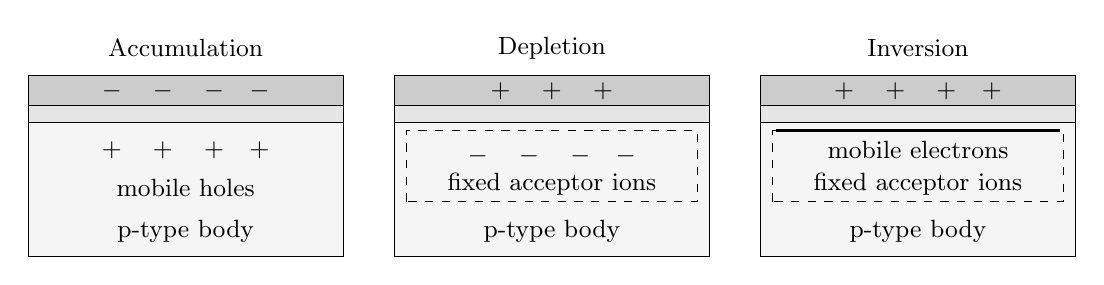
\begin{tikzpicture}[x=1cm,y=1cm,font=\small]
\foreach \x/\title in {0/Accumulation,4.65/Depletion,9.3/Inversion}{
 \draw[fill=gray!8] (\x,0) rectangle +(4,1.7);
 \draw[fill=gray!20] (\x,1.7) rectangle +(4,0.22);
 \draw[fill=gray!40] (\x,1.92) rectangle +(4,0.38);
 \node at (\x+2,2.65) {\title};
 \node at (\x+2,0.32) {p-type body};
}
\node at (2,2.1) {$-\quad-\quad-\quad-$};
\node at (2,1.35) {$+\quad+\quad+\quad+$};
\node at (2,0.87) {mobile holes};
\node at (6.65,2.1) {$+\quad+\quad+$};
\draw[dashed] (4.8,0.7) rectangle (8.5,1.6);
\node at (6.65,1.28) {$-\quad-\quad-\quad-$};
\node at (6.65,0.92) {fixed acceptor ions};
\node at (11.3,2.1) {$+\quad+\quad+\quad+$};
\draw[dashed] (9.45,0.7) rectangle (13.15,1.6);
\draw[very thick] (9.5,1.6)--(13.1,1.6);
\node at (11.3,1.36) {mobile electrons};
\node at (11.3,0.92) {fixed acceptor ions};
\end{tikzpicture}
\end{latin}
\caption{بازنمایی آموزشی سه وضعیت سطح \lr{MOS Capacitor} بر پایه شکل
\secnum{۲.۲} کتاب و اسلاید ۹. نوار میانی نازک، اکسید و نوار بالایی، \lr{Gate} است.
علامت‌های بار شماتیک‌اند و تعداد واقعی حامل‌ها را نشان نمی‌دهند \cite{weste,mos}.}
\label{fig:mos-surface}
\end{figure}

در \lr{Accumulation}، ولتاژ منفی \lr{Gate}، \lr{Hole}های مثبت را به سطح
جذب می‌کند. تراکم حامل غالب نزدیک سطح بیشتر می‌شود.
در \lr{Depletion}، ولتاژ مثبت کوچک \lr{Gate}، \lr{Hole}ها را از سطح دور
می‌کند و ناحیه‌ای با بار یون‌های منفی ثابت \lr{Acceptor} باقی می‌ماند.
در \lr{Inversion}، ولتاژ مثبت کافی، الکترون‌ها را به نزدیکی سطح می‌آورد و
لایه‌ای با حامل غالب الکترونی روی \lr{Body} نوع \lr{p} تشکیل می‌شود.
نوع حامل غالب در سطح تغییر می‌کند، درحالی‌که نوع \lr{Doping} کل \lr{Body} ثابت است.

\lr{Threshold Voltage} یا \(V_t\)، مرز قراردادی تشکیل \lr{Strong Inversion}
در این مدل است. مقدار آن به ساختار و \lr{Doping}، ضخامت اکسید و بایاس بستگی دارد.
در ترانزیستور \lr{Enhancement-mode nMOS} این درس، \(V_{tn}>0\) فرض می‌شود.
کتاب امکان مهندسی آستانه منفی را نیز یادآوری می‌کند.
در استخراج مقدماتی، \(V_t\) ثابت است و اثر بایاس \lr{Body} در بخش
\secnum{۲.۴} بررسی خواهد شد.

\subsection{پایانه‌ها، نمادها و جهت جریان}
چهار پایانه افزاره \lr{Gate}، \lr{Source}، \lr{Drain} و \lr{Body} هستند.
نماد سه‌پایانه اتصال \lr{Body} را به طور ضمنی نشان می‌دهد و در نماد چهارپایانه،
این اتصال آشکار است. کتاب در شکل \secnum{۲.۱} چند قرارداد رسم را نشان می‌دهد.
در نماد متداول اسلایدها، حباب روی \lr{Gate} رفتار معکوس \lr{pMOS} را مشخص می‌کند.
هنگام خواندن شکل، نوع افزاره و اتصال \lr{Body} را هم‌زمان بررسی می‌کنیم
\cite[صفحه ۶۱]{weste}.

هر ولتاژ دوپایانه‌ای، اختلاف پتانسیل پایانه اول و دوم است. تعریف‌ها چنین‌اند
\begin{equation}
 V_{GS}=V_G-V_S,\qquad V_{GD}=V_G-V_D,\qquad
 V_{DS}=V_D-V_S.
 \label{eq:mos-terminal-voltages}
\end{equation}
با کم‌کردن دو ولتاژ اول، \(V_G\) حذف می‌شود و داریم
\begin{equation*}
 V_{GS}-V_{GD}=(V_G-V_S)-(V_G-V_D)=V_D-V_S=V_{DS}.
\end{equation*}
این رابطه همان اسلاید ۱۰ است. برابرگرفتن \(V_{GS}\) با \(V_G\) هنگامی معتبر است
که \(V_S=0\) باشد.

در مدل متقارن مورد استفاده، برای \lr{nMOS} پایانه کم‌پتانسیل‌تر را
\lr{Source} می‌گیریم تا \(V_{DS}\ge0\) باشد. الکترون‌ها از \lr{Source} به
\lr{Drain} حرکت می‌کنند. به دلیل بار منفی الکترون، جریان قراردادی مثبت
\(I_{DS}\) از \lr{Drain} به \lr{Source} است. در \lr{pMOS}،
\lr{Source} پایانه پرپتانسیل‌تر و حرکت \lr{Hole} و جریان قراردادی از
\lr{Source} به \lr{Drain} است \cite[صفحه ۶۴]{weste}.

\subsection{تشخیص \lr{Cutoff}، \lr{Linear} و \lr{Saturation}}
برای \lr{nMOS} با \(V_{tn}>0\)، اگر \(V_{GS}<V_{tn}\) باشد، کانال
\lr{Strong Inversion} تشکیل نمی‌شود و افزاره در \lr{Cutoff} است.
مدل مرتبه اول جریان را صفر می‌گیرد. نشتی واقعی در بخش \secnum{۲.۴} بررسی می‌شود.
وقتی \(V_{GS}>V_{tn}\)، سمت \lr{Source} کانال تشکیل می‌شود.
اگر \(V_{DS}=0\)، با وجود کانال، اختلاف پتانسیل طولی و جریان خالص صفر است
\cite[شکل \secnum{۲.۳}]{weste}.

برای ولتاژ \lr{Drain} مثبت کوچک، کانال تا سمت \lr{Drain} ادامه دارد.
شرط تشکیل کانال در آن سمت \(V_{GD}>V_{tn}\) است.
با جای‌گذاری \(V_{GD}=V_{GS}-V_{DS}\)، این شرط به
\begin{equation}
 V_{DS}<V_{GS}-V_{tn}
 \label{eq:mos-linear-condition}
\end{equation}
تبدیل می‌شود. نام‌های \lr{Linear}، \lr{Triode}، \lr{Resistive} و
\lr{Nonsaturated} در کتاب برای این ناحیه به کار رفته‌اند.
تناسب تقریباً خطی جریان با \(V_{DS}\) هنگامی دقیق‌تر است که \(V_{DS}\) خیلی
کوچک‌تر از \(V_{GS}-V_{tn}\) باشد.

در مرز \(V_{DS}=V_{GS}-V_{tn}\)، اضافه‌ولتاژ مؤثر انتهای کانال صفر می‌شود.
با افزایش بیشتر \(V_{DS}\)، کانال در نزدیکی \lr{Drain} دچار \lr{Pinch-off}
می‌شود. حامل‌ها از انتهای کانال به ناحیه میدان قوی رسیده و به \lr{Drain}
منتقل می‌شوند. جریان برقرار می‌ماند. در مدل \lr{Long-channel} ایدئال، مقدار آن
برای \(V_{GS}\) ثابت تقریباً مستقل از \(V_{DS}\) است. این ناحیه
\lr{Saturation} نام دارد \cite[صفحات ۶۳ و ۶۴]{weste}.

شکل \ref{fig:mos-channel-shape} کاهش بار موضعی کانال از سمت \lr{Source}
به \lr{Drain} را نمایش می‌دهد. ضخامت ترسیمی، بزرگی بار را به طور شماتیک نشان می‌دهد.
\begin{figure}[ht]
\centering
\begin{latin}
\PersianMathDigits
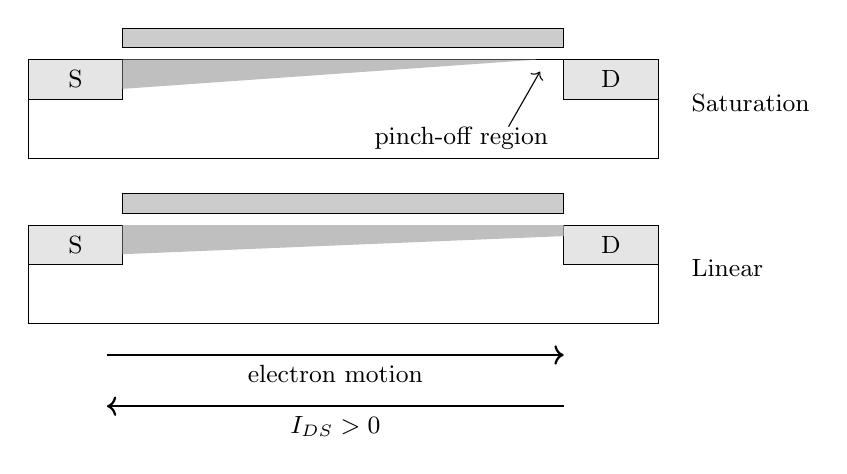
\begin{tikzpicture}[x=1cm,y=1cm,font=\small]
\foreach \y/\name in {0/Linear,2.1/Saturation}{
 \draw (0,\y) rectangle (8,\y+1.25);
 \draw[fill=gray!20] (0,\y+0.75) rectangle (1.2,\y+1.25);
 \draw[fill=gray!20] (6.8,\y+0.75) rectangle (8,\y+1.25);
 \draw[fill=gray!40] (1.2,\y+1.4) rectangle (6.8,\y+1.65);
 \draw (1.2,\y+1.25)--(6.8,\y+1.25);
 \node at (0.6,\y+1) {S};\node at (7.4,\y+1) {D};
 \node[anchor=west] at (8.3,\y+0.7) {\name};
}
\fill[gray!50] (1.2,1.25)--(6.8,1.25)--(6.8,1.11)--(1.2,0.88)--cycle;
\fill[gray!50] (1.2,3.35)--(6.45,3.35)--(1.2,2.98)--cycle;
\draw[->] (6.1,2.5)--(6.5,3.2);
\node at (5.5,2.35) {pinch-off region};
\draw[->,thick] (1,-0.4)--(6.8,-0.4) node[midway,below] {electron motion};
\draw[<-,thick] (1,-1.05)--(6.8,-1.05) node[midway,below] {$I_{DS}>0$};
\end{tikzpicture}
\end{latin}
\caption{نمای آموزشی کانال در دو ناحیه کاری، بر پایه شکل \secnum{۲.۳} کتاب.
کانال نزدیک \lr{Drain} بار کمتری دارد. در \lr{Saturation} حامل‌ها از ناحیه
\lr{Pinch-off} به \lr{Drain} انتقال می‌یابند \cite{weste}.}
\label{fig:mos-channel-shape}
\end{figure}

برای اختصار، \lr{Overdrive Voltage} را مطابق نماد کتاب به صورت
\(V_{GT}=V_{GS}-V_{tn}\) تعریف می‌کنیم. جدول \ref{tab:mos-regions} روند انتخاب
ناحیه را خلاصه می‌کند. در مدل قطعه‌ای، نقطه آستانه را با جریان صفر به
\lr{Cutoff} و مرز \lr{Linear} و \lr{Saturation} را به ناحیه دوم نسبت می‌دهیم.
دو رابطه جریان در مرز دوم یک مقدار می‌دهند.
\clearpage
\begin{table}[ht]
\centering
\caption{ناحیه‌های \lr{nMOS} با فرض \(V_{DS}\ge0\) و آستانه ثابت.}
\label{tab:mos-regions}
\begin{tabularx}{\textwidth}{rXX}
\toprule
ناحیه & شرط & تفسیر\\
\midrule
\lr{Cutoff} & \(V_{GS}\le V_{tn}\) & جریان صفر در مدل مرتبه اول\\
\lr{Linear} & \(V_{GS}>V_{tn},\ 0\le V_{DS}<V_{GT}\) & کانال تا دو انتها برقرار است\\
\lr{Saturation} & \(V_{GS}>V_{tn},\ V_{DS}\ge V_{GT}\) & جریان ایدئال با ولتاژ \lr{Gate} تعیین می‌شود\\
\bottomrule
\end{tabularx}
\end{table}

\subsection{مثال‌های تشخیص ناحیه با \lr{Source} غیرصفر}
در مثال‌های فرضی این قسمت، \(V_{tn}=\qty{0.4}{\volt}\) ثابت است.
اگر \(V_G=\qty{1.2}{\volt}\)، \(V_S=\qty{0.3}{\volt}\) و
\(V_D=\qty{0.5}{\volt}\) باشند، ابتدا اختلاف‌ها را حساب می‌کنیم
\[
 V_{GS}=1.2-0.3=\qty{0.9}{\volt},\qquad
 V_{DS}=0.5-0.3=\qty{0.2}{\volt},\qquad
 V_{GT}=0.9-0.4=\qty{0.5}{\volt}.
\]
چون \(V_{GS}>V_{tn}\) و \(0.2<0.5\)، ناحیه \lr{Linear} است.
از سوی دیگر \(V_{GD}=1.2-0.5=\qty{0.7}{\volt}>V_{tn}\) نیز همان نتیجه را تأیید می‌کند.

اگر تنها \(V_D\) به \qty{1.0}{\volt} تغییر کند، \(V_{DS}=\qty{0.7}{\volt}\)
و \(V_{GD}=\qty{0.2}{\volt}\) می‌شوند. شرط \(V_{DS}\ge V_{GT}\) برقرار است
و ترانزیستور در \lr{Saturation} قرار می‌گیرد. اگر در حالت دیگری
\(V_G=\qty{0.6}{\volt}\) باشد و \(V_S=\qty{0.3}{\volt}\) باقی بماند،
\(V_{GS}=\qty{0.3}{\volt}<V_{tn}\) و ترانزیستور در \lr{Cutoff} است.
شرط روشن‌شدن پیش از مقایسه \(V_{DS}\) با \(V_{GT}\) بررسی می‌شود.

برای \lr{Body} ثابت و \lr{Source} متحرک، آستانه واقعی می‌تواند با
\lr{Body Effect} تغییر کند. این سه مثال برای تمرین اختلاف ولتاژ، آستانه را
ثابت فرض کرده‌اند. تحلیل اثر بایاس \lr{Body} در دامنه بخش \secnum{۲.۴} است.
\subsection{ولتاژ تغذیه و محدودیت اکسید}
\(V_{DD}\) ولتاژ ریل تغذیه نسبت به \lr{GND} با مرجع صفر است.
اسلاید ۲۵، تغذیه \qty{5}{\volt} در مثال تاریخی دهه ۱۹۸۰ و کاهش ولتاژ در
فناوری‌های مورد بحث خود را نشان می‌دهد \cite{mos}.
با نازک‌شدن اکسید، همان اختلاف ولتاژ می‌تواند میدان عمودی بزرگ‌تری ایجاد کند.
در مدل یکنواخت، بزرگی میدان اکسید تقریباً \(E_{\mathrm{ox}}=V_{\mathrm{ox}}/t_{\mathrm{ox}}\)
است، که \(V_{\mathrm{ox}}\) ولتاژ دو سوی خود اکسید است.
انتخاب تغذیه باید با محدودیت افزاره و مشخصات فناوری سازگار باشد.
کاهش ولتاژ در رابطه توان دینامیکی، انرژی هر شارژ را کاهش می‌دهد.
هم‌زمان، جریان و زمان تغییر ولتاژ مدار نیز با نقطه بایاس تغییر می‌کنند.
این وابستگی، سرعت، توان و قابلیت اطمینان را به انتخاب مشترک ولتاژ مرتبط می‌کند.
\clearpage

\section{استخراج و کاربرد روابط \lr{Long-channel I-V}}
\label{sec:book-mos-current}
\subsection{فرض‌های مدل و معنای پارامترها}
مدل \lr{Long-channel} را \lr{Ideal}، \lr{First-order} یا \lr{Shockley Model}
نیز می‌نامند. کانال به اندازه‌ای بلند فرض می‌شود که مدل سرعت متناسب با میدان
طولی قابل‌استفاده باشد. \lr{Mobility}، ضخامت مؤثر اکسید و آستانه را در این تحلیل
ثابت می‌گیریم. جریان \lr{Gate} و جریان حالت خاموش صفر فرض می‌شوند. اثرهای
\lr{Velocity Saturation}، \lr{Mobility Degradation} و \lr{Channel Length Modulation}
در بخش \secnum{۲.۴} به تحلیل افزوده می‌شوند \cite[صفحات ۶۴ و ۶۵]{weste}.

در مدل کانال تدریجی، تغییر پتانسیل در امتداد کانال نسبت به تغییر عمودی آن آرام
فرض می‌شود. در نتیجه، بار موضعی را می‌توان با یک رابطه خازنی تقریب زد.
برای محاسبه حاضر، تأثیر تغییر بایاس محلی بر بار \lr{Depletion} در یک آستانه ثابت
خلاصه می‌شود. این فرض‌ها دامنه کاربرد روابط را تعیین می‌کنند.
نمادهای جدول \ref{tab:mos-parameters} پیش از استخراج به کار می‌روند.
\begin{table}[ht]
\centering
\caption{نمادها و واحدهای روابط جریان.}
\label{tab:mos-parameters}
\begin{tabularx}{\textwidth}{rXr}
\toprule
نماد & تعریف & واحد نمونه\\
\midrule
\(W,L\) & عرض کانال و طول مسیر میان \lr{Source} و \lr{Drain} & \unit{\metre}\\
\(t_{\mathrm{ox}}\) & ضخامت اکسید یا ضخامت معادل تعریف‌شده & \unit{\metre}\\
\(\varepsilon_{\mathrm{ox}}\) & \lr{Permittivity} اکسید & \unit{\farad\per\metre}\\
\(C_{\mathrm{ox}}\) & ظرفیت اکسید بر واحد سطح & \unit{\farad\per\metre\squared}\\
\(C_g\) & ظرفیت مدل صفحه‌ای \lr{Gate} و کانال & \unit{\farad}\\
\(\mu_n,\mu_p\) & \lr{Mobility} الکترون و \lr{Hole} & \unit{\metre\squared\per\volt\per\second}\\
\(\beta\) & ضریب فناوری و هندسه در رابطه جریان & \unit{\ampere\per\volt\squared}\\
\(V_{GT}\) & اضافه‌ولتاژ \(V_{GS}-V_{tn}\) در \lr{nMOS} & \unit{\volt}\\
\bottomrule
\end{tabularx}
\end{table}

\subsection{ظرفیت اکسید، هندسه و \lr{EOT}}
طول \(L\) در راستای حرکت حامل از \lr{Source} به \lr{Drain} و عرض \(W\)
در راستای عمود بر آن، روی سطح کانال اندازه‌گیری می‌شود.
در \lr{Strong Inversion}، \lr{Gate} و کانال در دو سوی عایق، تقریباً یک خازن
صفحه‌ای می‌سازند. مساحت مؤثر هندسی \(WL\) است و برای اکسید \lr{SiO\(_2\)} داریم
\begin{equation}
 \varepsilon_{\mathrm{ox}}=3.9\varepsilon_0,\qquad
 C_{\mathrm{ox}}=\frac{\varepsilon_{\mathrm{ox}}}{t_{\mathrm{ox}}},\qquad
 C_g=C_{\mathrm{ox}}WL.
 \label{eq:mos-oxide-cap}
\end{equation}
\(\varepsilon_0\approx\qty{8.85e-12}{\farad\per\metre}\) است.
در واحد سانتی‌متری کتاب، همین مقدار
\qty{8.85e-14}{\farad\per\centi\metre} نوشته می‌شود
\cite[رابطه \secnum{۲.۲}، شکل \secnum{۲.۶}]{weste}.
با نصف‌شدن ضخامت، ظرفیت بر واحد سطح دو برابر می‌شود. با دوبرابرشدن عرض، ظرفیت
کل دو برابر می‌شود. \(C_{\mathrm{ox}}\) و \(C_g\) واحد و نقش متفاوتی دارند.

برای نمونه فرضی \(t_{\mathrm{ox}}=\qty{10}{\nano\metre}\)،
\(W=\qty{1}{\micro\metre}\) و \(L=\qty{0.5}{\micro\metre}\)، ابتدا همه طول‌ها
را به متر می‌بریم. چون \(\qty{10}{\nano\metre}=10^{-8}\,\unit{\metre}\)، داریم
\begin{align*}
 C_{\mathrm{ox}}&=\frac{3.9(8.85\times10^{-12})}{10^{-8}}
 =3.4515\times10^{-3}\,\unit{\farad\per\metre\squared},\\
 C_g&=(3.4515\times10^{-3})(10^{-6})(0.5\times10^{-6})\,\unit{\farad}
 \approx\qty{1.73}{\femto\farad}.
\end{align*}
ضریب تبدیل مساحت از \unit{\micro\metre\squared} به \unit{\metre\squared}
برابر \(10^{-12}\) است، زیرا هر دو بعد در \(10^{-6}\) ضرب می‌شوند.
این ظرفیت صفحه‌ای، پایه استخراج جریان است. تقسیم آن میان پایانه‌ها در بخش
\secnum{۲.۳} بررسی می‌شود.

برای عایق \lr{High-k}، \lr{Equivalent Oxide Thickness} یا \lr{EOT} را ضخامت
لایه فرضی \lr{SiO\(_2\)} با همان \(C_{\mathrm{ox}}\) تعریف می‌کنند
\cite[صفحه ۶۶]{weste}. اگر ضخامت فیزیکی عایق \(t_h\) و گذردهی آن
\(\varepsilon_h\) باشد، از برابرگرفتن ظرفیت بر واحد سطح نتیجه می‌شود
\begin{equation}
 \frac{\varepsilon_h}{t_h}=\frac{\varepsilon_{\mathrm{ox}}}{\mathrm{EOT}}
 \quad\Longrightarrow\quad
 \mathrm{EOT}=t_h\frac{\varepsilon_{\mathrm{ox}}}{\varepsilon_h}.
 \label{eq:mos-eot}
\end{equation}
اگر گذردهی چهار برابر و ضخامت فیزیکی \qty{4}{\nano\metre} باشد،
\(\mathrm{EOT}=\qty{1}{\nano\metre}\) می‌شود. در این مثال، ضخامت فیزیکی بیشتر
با ظرفیت معادل همان اکسید نازک سازگار است.

\subsection{بار کانال در توضیح متوسط کتاب}
بار روی خازن به ولتاژ دو سوی همان خازن وابسته است. پتانسیل کانال میان
\(V_S\) و \(V_D\) تغییر می‌کند. کتاب برای استخراج مقدماتی، پتانسیل نماینده کانال
را میانگین دو انتها می‌گیرد و می‌نویسد
\begin{align}
 V_c&\approx\frac{V_S+V_D}{2}=V_S+\frac{V_{DS}}2,\notag\\
 V_{gc}&\approx V_G-V_c=V_{GS}-\frac{V_{DS}}2.
 \label{eq:mos-mean-potential}
\end{align}
برای تشکیل بار متحرک، ولتاژ باید از آستانه عبور کند. با تعریف بزرگی بار کانال
\(Q_{\mathrm{ch}}\ge0\)، رابطه مقدماتی کتاب چنین بازنویسی می‌شود
\begin{equation}
 Q_{\mathrm{ch}}\approx C_g(V_{gc}-V_{tn})
 \approx C_{\mathrm{ox}}WL\left(V_{GT}-\frac{V_{DS}}2\right).
 \label{eq:mos-average-charge}
\end{equation}
این توضیح از رابطه \secnum{۲.۱} کتاب و اسلاید ۱۵ گرفته شده است.
علامت بار الکترون‌ها منفی است. در این رابطه با بزرگی آن کار می‌کنیم.
افزایش \(V_{GS}\) بار متحرک را بیشتر می‌کند. افزایش \(V_{DS}\) با ثابت‌ماندن
\(V_{GS}\)، اضافه‌ولتاژ مؤثر نزدیک \lr{Drain} را کم می‌کند.

میانگین دو ولتاژ انتهایی یک ساده‌سازی برای استخراج مقدماتی است.
پتانسیل واقعی در طول کانال الزاماً خطی با مکان تغییر نمی‌کند، بنابراین
\eqref{eq:mos-average-charge} را به عنوان تقریب بزرگی کل بار به کار می‌بریم.
استخراج با بار موضعی در ادامه، همان رابطه جریان را در مدل کانال تدریجی به دست می‌دهد
و نیاز به فرض خطی‌بودن پتانسیل مکانی را برمی‌دارد.

\subsection{\lr{Mobility}، میدان طولی و زمان عبور}
\lr{Mobility} ضریب تبدیل بزرگی میدان الکتریکی به سرعت متوسط رانش در مدل میدان
کم است. اگر \(v\) بزرگی سرعت و \(E\) بزرگی میدان طولی باشد، داریم
\begin{equation}
 v=\mu_n E,\qquad E\approx\frac{V_{DS}}L,\qquad
 t_{\mathrm{tr}}\approx\frac Lv.
 \label{eq:mos-drift}
\end{equation}
رابطه‌های \secnum{۲.۳} و \secnum{۲.۴} کتاب و اسلاید ۱۶ همین مسیر را بیان می‌کنند.
\(t_{\mathrm{tr}}\) زمان عبور حامل در این تصویر مقدماتی است. تأخیر گیت به جریان
شارژ و تخلیه بار خارجی نیز وابسته است.

برای فهم واحد \(\mu\)، میدان واحد \unit{\volt\per\metre} دارد و سرعت واحد
\unit{\metre\per\second}. پس واحد ضریب تناسب
\unit{\metre\squared\per\volt\per\second} است. تبدیل واحد رایج کتاب چنین است
\begin{equation*}
 \qty{1}{\centi\metre\squared\per\volt\per\second}
 =10^{-4}\,\unit{\metre\squared\per\volt\per\second}.
\end{equation*}
کتاب برای الکترون در میدان کم حدود \num{500} تا
\qty{700}{\centi\metre\squared\per\volt\per\second}
را ذکر می‌کند و سپس کاهش \lr{Mobility} در میدان‌های قوی را یادآور می‌شود
\cite[صفحه ۶۶]{weste}. مقدار مناسب هر مثال باید از داده همان مثال برداشته شود.

در مثال فرضی \(L=\qty{1}{\micro\metre}\)، \(V_{DS}=\qty{0.1}{\volt}\)
و \(\mu_n=\qty{500}{\centi\metre\squared\per\volt\per\second}\)، داریم
\[
 E\approx\frac{0.1}{10^{-6}}=10^5\,\unit{\volt\per\metre},\qquad
 v\approx(0.05)(10^5)=\qty{5000}{\metre\per\second},\qquad
 t_{\mathrm{tr}}\approx\qty{0.2}{\nano\second}.
\]
در این محاسبه، تناسب سرعت با میدان و تقریب میدان متوسط فرض شده‌اند.

\subsection{استخراج رابطه \lr{Linear} با روش کتاب}
جریان، بار عبوری در واحد زمان است. در تصویر بار متوسط و زمان عبور متوسط،
جریان برابر \(Q_{\mathrm{ch}}/t_{\mathrm{tr}}\) تخمین زده می‌شود.
با جای‌گذاری \eqref{eq:mos-average-charge} و \eqref{eq:mos-drift}، مراحل حذف
عامل‌ها را به صورت زیر دنبال می‌کنیم
\begin{align}
 I_{DS}&\approx\frac{Q_{\mathrm{ch}}}{L/v}
 =Q_{\mathrm{ch}}\frac vL,\notag\\
 &\approx C_{\mathrm{ox}}WL\left(V_{GT}-\frac{V_{DS}}2\right)
 \frac{\mu_n V_{DS}}{L^2},\notag\\
 &=\mu_n C_{\mathrm{ox}}\frac WL
 \left(V_{GT}V_{DS}-\frac{V_{DS}^2}{2}\right).
 \label{eq:mos-book-linear}
\end{align}
از یک عامل \(L\) در صورت و دو عامل \(L\) در مخرج، نسبت \(1/L\) باقی می‌ماند.
با معرفی پارامتر فناوری \(k'_n\) و پارامتر فناوری و هندسه \(\beta_n\)، داریم
\begin{equation}
 k'_n=\mu_n C_{\mathrm{ox}},\qquad
 \beta_n=k'_n\frac WL=\mu_n C_{\mathrm{ox}}\frac WL.
 \label{eq:mos-beta}
\end{equation}
پس رابطه مدل برای \(V_{GS}>V_{tn}\) و \(0\le V_{DS}\le V_{GT}\) چنین است
\begin{equation}
 \boxed{I_{DS}=\beta_n\left[(V_{GS}-V_{tn})V_{DS}-\frac{V_{DS}^2}{2}\right].}
 \label{eq:mos-linear}
\end{equation}
این رابطه با روابط \secnum{۲.۵} تا \secnum{۲.۷} کتاب و اسلاید ۱۷ سازگار است.
علامت مساوی در \eqref{eq:mos-linear} بیانگر رابطه تعریف‌شده در مدل ایدئال است.

واحد \(\mu C_{\mathrm{ox}}\) برابر
\(\unit{\farad\per\volt\per\second}=\unit{\ampere\per\volt\squared}\) است.
نسبت \(W/L\) بی‌بعد است. داخل کروشه دو جمله با واحد \unit{\volt\squared}
داریم و حاصل، جریان با واحد \unit{\ampere} است.
برخی منابع، عامل \(1/2\) را در تعریف \(k'\) یا ضریب جریان جذب می‌کنند.
پانوشت صفحه ۶۶ کتاب نیز این تفاوت را یادآوری می‌کند.
پیش از استفاده از مقدار نقل‌شده، تعریف ضریب را با \eqref{eq:mos-beta} مقایسه می‌کنیم.

\subsection{استخراج تکمیلی با بار موضعی و انتگرال}
برای دقیق‌ترکردن استدلال در چارچوب همان مدل، مکان \(x\) را از \lr{Source}
در \(x=0\) تا \lr{Drain} در \(x=L\) تعریف می‌کنیم. \(V(x)\) پتانسیل محلی
نسبت به \lr{Source} است. پس \(V(0)=0\) و \(V(L)=V_{DS}\).
در قطعه کوچکی به طول \(dx\)، بزرگی بار متحرک کانال برابر است با
\begin{equation}
 dQ_{\mathrm{ch}}=W C_{\mathrm{ox}}[V_{GT}-V(x)]\,dx.
 \label{eq:mos-local-charge}
\end{equation}
عبارت \(C_{\mathrm{ox}}[V_{GT}-V(x)]\) بار بر واحد سطح و
\(Wdx\) سطح قطعه است. بار علامت‌دار الکترون‌ها، منفی این مقدار است.

زمان عبور از همین قطعه \(dt=dx/v(x)\) و بزرگی سرعت رانش
\(v(x)=\mu_n\,dV/dx\) است. این رابطه از بزرگی میدان استفاده می‌کند.
با تقسیم بار عبوری بر زمان و فرض جریان پایدار در طول کانال، داریم
\begin{equation}
 I_{DS}=W\mu_nC_{\mathrm{ox}}[V_{GT}-V(x)]\frac{dV}{dx}.
 \label{eq:mos-local-current}
\end{equation}
در جریان پایدار، بار در هیچ قطعه‌ای انباشته نمی‌شود، بنابراین جریان عبوری از
همه مقطع‌ها یکسان است. دو طرف را در \(dx\) ضرب و در طول کانال جمع می‌کنیم.
نماد انتگرال، جمع پیوسته سهم قطعه‌های کوچک است. با تغییر متغیر از مکان به
پتانسیل، جمع از صفر تا \(V_{DS}\) انجام می‌شود
\begin{equation*}
 \int_0^L I_{DS}\,dx
 =W\mu_nC_{\mathrm{ox}}\int_0^{V_{DS}}(V_{GT}-V)\,dV.
\end{equation*}
سمت چپ چون جریان ثابت است، \(I_{DS}L\) می‌شود. در سمت راست، مساحت زیر خط
\(V_{GT}-V\) در بازه صفر تا \(V_{DS}\)، مساحت یک مستطیل به ارتفاع \(V_{GT}\)
منهای مساحت مثلث به ارتفاع و قاعده \(V_{DS}\) است. پس
\begin{equation*}
 I_{DS}L=W\mu_n C_{\mathrm{ox}}
 \left(V_{GT}V_{DS}-\frac12V_{DS}^2\right).
\end{equation*}
تقسیم بر \(L\)، دقیقاً رابطه \eqref{eq:mos-linear} را در فرض‌های مدل به دست
می‌دهد. عامل یک‌دوم از تغییر بار در امتداد کانال ناشی می‌شود. شرط
\(V_{DS}\le V_{GT}\) تضمین می‌کند بار موضعی در سراسر کانال نامنفی باقی بماند.

\subsection{تقریب مقاومتی و مرز \lr{Saturation}}
برای \(V_{DS}\ll V_{GT}\)، جمله مربعی نسبت به جمله اول کوچک است. نسبت بزرگی
آن دو جمله \(V_{DS}/(2V_{GT})\) است. با حذف جمله کوچک، داریم
\begin{equation}
 I_{DS}\approx\beta_nV_{GT}V_{DS},\qquad
 R_{\mathrm{on}}\approx\frac{V_{DS}}{I_{DS}}
 \approx\frac1{\beta_nV_{GT}}.
 \label{eq:mos-small-vds}
\end{equation}
مقاومت تقریبی با ولتاژ \lr{Gate} کنترل می‌شود.
در رابطه کامل ناحیه \lr{Linear}، نسبت \(V_{DS}/I_{DS}\) برابر
\(1/[\beta_n(V_{GT}-V_{DS}/2)]\) است و با ولتاژ تغییر می‌کند.

برای \(\beta_n=\qty{200}{\micro\ampere\per\volt\squared}\)،
\(V_{GT}=\qty{0.8}{\volt}\) و \(V_{DS}=\qty{0.1}{\volt}\)، جریان کامل
به صورت زیر محاسبه می‌شود.
\[
 200[0.8(0.1)-0.1^2/2]=\qty{15}{\micro\ampere}.
\]
تقریب مقاومتی \qty{16}{\micro\ampere} می‌دهد، حدود \num{6.7} درصد بیشتر از مقدار
رابطه کامل. برای کاهش خطای این تقریب باید نسبت \(V_{DS}/V_{GT}\) کوچک‌تر شود.

در مرز تشکیل \lr{Pinch-off}، \(V_{GD}=V_{tn}\)، بنابراین ولتاژ اشباع در مدل
بلندکانال برابر است با
\begin{equation}
 V_{DS,\mathrm{sat}}=V_{GT}=V_{GS}-V_{tn}.
 \label{eq:mos-vdsat}
\end{equation}
با جای‌گذاری همین مقدار در \eqref{eq:mos-linear}، داریم
\begin{align}
 I_{DS,\mathrm{sat}}
 &=\beta_n\left(V_{GT}^2-\frac{V_{GT}^2}{2}\right)
 =\frac{\beta_n}{2}V_{GT}^2,\notag\\
 &\boxed{I_{DS,\mathrm{sat}}=\frac{\beta_n}{2}(V_{GS}-V_{tn})^2.}
 \label{eq:mos-saturation}
\end{align}
این رابطه برای \(V_{GS}>V_{tn}\) و \(V_{DS}\ge V_{DS,\mathrm{sat}}\) به کار
می‌رود \cite[رابطه \secnum{۲.۸} و اسلاید ۱۸]{weste,mos}.
پس از مرز، افزایش ولتاژ \lr{Drain} عمدتاً روی ناحیه نزدیک \lr{Drain} می‌افتد.
در تقریبِ طول مؤثر ثابت، جریان به مقدار مرزی محدود می‌شود.

می‌توان رابطه \lr{Linear} را با کامل‌کردن مربع نیز بازنوشت
\begin{equation}
 I_{DS}=\frac{\beta_n}{2}
 \left[V_{GT}^2-(V_{GT}-V_{DS})^2\right],\qquad 0\le V_{DS}\le V_{GT}.
 \label{eq:mos-complete-square}
\end{equation}
در مرز، مربع دوم صفر و جریان برابر بیشینه این قطعه است.
برای \(V_{DS}>V_{GT}\)، فرض بار نامنفی تا انتهای کانال از اعتبار می‌افتد و
قطعه اشباع انتخاب می‌شود. همین انتخاب از افت مصنوعی جریان ناشی از ادامه‌دادن
سهمی به بیرون بازه جلوگیری می‌کند.

\subsection{رابطه قطعه‌ای، پیوستگی و جریان‌های \lr{Ion} و \lr{Ioff}}
برای \(V_{DS}\ge0\)، مدل جریان را با شرط‌ها یکجا می‌نویسیم
\begin{equation}
 I_{DS}=\begin{cases}
 0,&V_{GS}\le V_{tn},\\[2pt]
 \beta_n(V_{GT}V_{DS}-V_{DS}^2/2),
 &V_{GS}>V_{tn},\quad 0\le V_{DS}<V_{GT},\\[2pt]
 \beta_n V_{GT}^2/2,
 &V_{GS}>V_{tn},\quad V_{DS}\ge V_{GT}.
 \end{cases}
 \label{eq:mos-piecewise}
\end{equation}
این صورت، مرزهای رابطه \secnum{۲.۱۰} کتاب و اسلاید ۱۹ را نیز پوشش می‌دهد.
در \(V_{DS}=0\)، قطعه \lr{Linear} جریان صفر می‌دهد. در
\(V_{DS}=V_{GT}\)، دو قطعه مقدار \(\beta_n V_{GT}^2/2\) می‌دهند.
با \(V_{GS}\) نزدیک آستانه از بالا، جریان اشباع به صفر میل می‌کند.
در هر سه بررسی، رفتار قطعه‌ای پیوسته است.

کتاب \(I_{\mathrm{on}}\) را جریان در \(V_{GS}=V_{DS}=V_{DD}\)، و
\(I_{\mathrm{off}}\) را جریان در \(V_{GS}=0,V_{DS}=V_{DD}\) تعریف می‌کند.
برای \(V_{DD}>V_{tn}>0\)، شرط اشباع برای حالت روشن برقرار است و داریم
\begin{equation}
 I_{\mathrm{on}}=\frac{\beta_n}{2}(V_{DD}-V_{tn})^2,\qquad
 I_{\mathrm{off}}=0\quad\text{\rl{در مدل مرتبه اول}}.
 \label{eq:mos-ion-ioff}
\end{equation}
اگر \(V_{DD}\le V_{tn}\) باشد، همین مدل جریان حالت روشن را نیز صفر می‌گیرد.
این شرط پیش از مربع‌کردن اختلاف بررسی می‌شود. جریان خاموش واقعی در درس
\lr{Leakage} تحلیل خواهد شد \cite[رابطه \secnum{۲.۹}]{weste}.

در \lr{Saturation}، دوبرابرشدن \(W\) با بقیه پارامترهای ثابت، جریان را دو برابر
می‌کند. دوبرابرشدن \(L\) جریان را نصف می‌کند، مشروط به حفظ اعتبار مدل و پارامترها.
دوبرابرشدن \(V_{GT}\) جریان را چهار برابر می‌کند. برای تغییر \(V_{GS}\)،
ابتدا آستانه را کم می‌کنیم و سپس توان دو می‌گیریم.
\clearpage

\subsection{حل مثال اسلاید ۲۰ با واحدهای سازگار}
داده‌های اسلاید ۲۰ عبارت‌اند از \(t_{\mathrm{ox}}=\qty{10}{\nano\metre}\)،
\(\mu_n=\qty{350}{\centi\metre\squared\per\volt\per\second}\)،
\(V_{tn}=\qty{0.7}{\volt}\) و \(W/L=4/2=2\) \cite{mos}.
در اسلاید، ضخامت به صورت \(100\) \lr{angstrom} داده شده است.
هر \lr{angstrom} برابر \(10^{-10}\,\unit{\metre}\) است، پس
\(100\) \lr{angstrom} برابر \qty{10}{\nano\metre} می‌شود.

با واحد متر، \(\mu_n=0.035\,\unit{\metre\squared\per\volt\per\second}\)
و \(C_{\mathrm{ox}}=3.4515\times10^{-3}\,\unit{\farad\per\metre\squared}\) است.
بنابراین
\begin{align*}
 k'_n&=(0.035)(3.4515\times10^{-3})\,
 \unit{\ampere\per\volt\squared}
 \approx\qty{120.8}{\micro\ampere\per\volt\squared},\\
 \beta_n&=k'_n\frac WL\approx\qty{241.6}{\micro\ampere\per\volt\squared}.
\end{align*}
اسلاید ضریب \(k'_n\) را حدود \qty{120}{\micro\ampere\per\volt\squared}
گزارش می‌کند. برای هماهنگی با دقت همان مثال، در ادامه
\(\beta_n=\qty{240}{\micro\ampere\per\volt\squared}\) می‌گیریم.
وقتی \(V_{GS}=\qty{3}{\volt}\)، اضافه‌ولتاژ \(V_{GT}=\qty{2.3}{\volt}\) است.
برای \(V_{DS}=\qty{1}{\volt}\)، ناحیه \lr{Linear} و جریان
\[
 I_{DS}=240\left[2.3(1)-\frac{1^2}{2}\right]\,\unit{\micro\ampere}
 =\qty{432}{\micro\ampere}
\]
می‌شود. برای \(V_{DS}=\qty{4}{\volt}\)، ناحیه \lr{Saturation} و جریان
\[
 I_{DS}=\frac{240}{2}(2.3)^2\,\unit{\micro\ampere}
 =\qty{634.8}{\micro\ampere}\approx\qty{0.635}{\milli\ampere}
\]
است. مقدار \(V_{DS}=\qty{2.3}{\volt}\) در هر دو فرمول همین پاسخ را می‌دهد.
منحنی‌های شکل \ref{fig:mos-slide-curves} با همین ضریب گرد‌شده محاسبه شده‌اند.

\begin{figure}[ht]
\centering
\begin{latin}
\PersianMathDigits
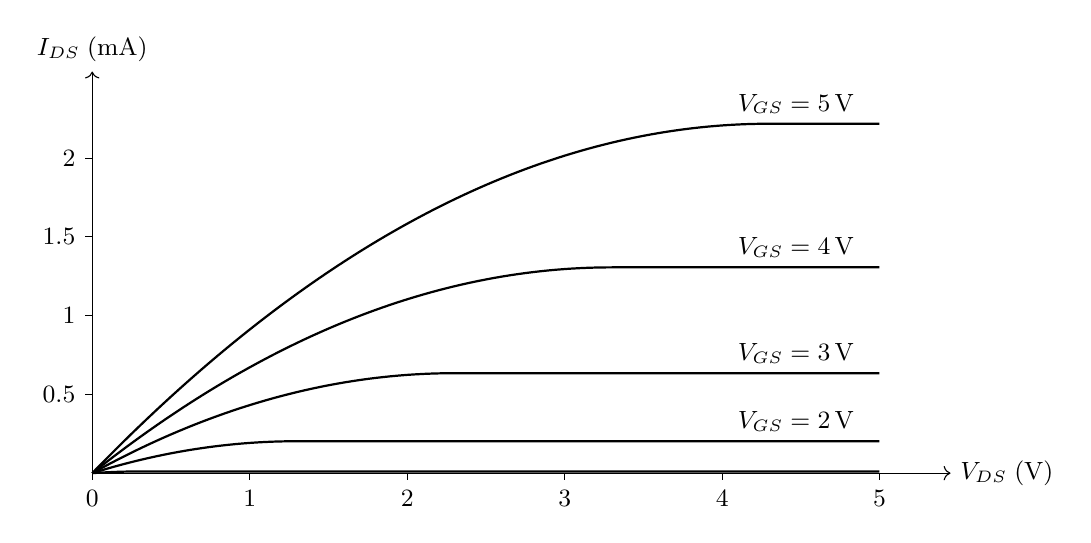
\begin{tikzpicture}[x=2cm,y=2cm,font=\small]
\draw[->] (0,0)--(5.45,0) node[right] {$V_{DS}\;(\mathrm V)$};
\draw[->] (0,0)--(0,2.55) node[above] {$I_{DS}\;(\mathrm{mA})$};
\foreach \x in {0,1,2,3,4,5}{\draw (\x,0)--(\x,-0.045) node[below] {$\x$};}
\foreach \y in {0.5,1,1.5,2}{\draw (0,\y)--(-0.045,\y) node[left] {$\y$};}
\foreach \g in {1,2,3,4,5}{
 \draw[thick,domain=0:5,samples=101] plot (\x,{0.24*((\g-0.7)*min(\x,\g-0.7)-0.5*min(\x,\g-0.7)^2)});
}
\node[anchor=south east] at (4.9,2.22) {$V_{GS}=5\,\mathrm V$};
\node[anchor=south east] at (4.9,1.307) {$V_{GS}=4\,\mathrm V$};
\node[anchor=south east] at (4.9,0.635) {$V_{GS}=3\,\mathrm V$};
\node[anchor=south east] at (4.9,0.203) {$V_{GS}=2\,\mathrm V$};
\end{tikzpicture}
\end{latin}
\caption{مشخصه‌های محاسبه‌شده از مدل \lr{Long-channel} با داده اسلاید ۲۰ و
\(\beta_n=\qty{240}{\micro\ampere\per\volt\squared}\). منحنی \(V_{GS}=0\)
روی محور افقی است و پایین‌ترین منحنی غیرصفر به \(V_{GS}=\qty{1}{\volt}\) مربوط است.
نمودار، بازتولید مدل ایدئال با فرض‌های بیان‌شده است \cite{mos}.}
\label{fig:mos-slide-curves}
\end{figure}

\subsection{حل مثال \texorpdfstring{\secnum{۲.۱}}{۲.۱} کتاب و اختلاف عدد ضریب}
در مثال \secnum{۲.۱} کتاب، نام فناوری \qty{65}{\nano\metre} است، اما طول رسم‌شده
\(L=\qty{50}{\nano\metre}\) و \(W=\qty{100}{\nano\metre}\) داده شده است.
برای محاسبه \(W/L\)، ابعاد واقعی داده‌شده را به کار می‌بریم. سایر داده‌ها
\(t_{\mathrm{ox}}=\qty{1.05}{\nano\metre}\)،
\(\mu_n=\qty{80}{\centi\metre\squared\per\volt\per\second}\) و
\(V_{tn}=\qty{0.3}{\volt}\) در دمای ذکرشده \qty{70}{\degreeCelsius} هستند
\cite[صفحه ۶۷]{weste}.

تبدیل‌ها \(\mu_n=0.008\,\unit{\metre\squared\per\volt\per\second}\)،
\(t_{\mathrm{ox}}=1.05\times10^{-9}\,\unit{\metre}\) و \(W/L=2\) می‌دهند.
پس با ثابت \(\varepsilon_0\) درج‌شده در کتاب داریم
\begin{align}
 C_{\mathrm{ox}}&=\frac{3.9(8.85\times10^{-12})}{1.05\times10^{-9}}
 \approx0.03287\,\unit{\farad\per\metre\squared},\notag\\
 k'_n&\approx(0.008)(0.03287)
 \approx\qty{263}{\micro\ampere\per\volt\squared},\notag\\
 \beta_n&\approx\qty{526}{\micro\ampere\per\volt\squared}.
 \label{eq:mos-book-beta}
\end{align}
در رابطه \secnum{۲.۱۱} چاپ کتاب، ضریب پیش از \(W/L\) برابر
\qty{262}{\micro\ampere\per\volt\squared} نوشته شده است.
محاسبه از داده‌های درج‌شده حدود \qty{263}{\micro\ampere\per\volt\squared}
می‌دهد. اختلاف حدود \num{0.4} درصد است. برای سازگاری داخلی، جدول و نمودار این جزوه
همگی با \(\beta_n=\qty{526}{\micro\ampere\per\volt\squared}\) محاسبه شده‌اند.

برای \(V_{GS}=0\) و \qty{0.2}{\volt}، شرط روشن‌شدن برقرار نیست.
برای چهار مقدار بعدی، جدول \ref{tab:mos-book-points} ولتاژ مرزی و جریان اشباع
را نشان می‌دهد. مثلاً در \(V_{GS}=\qty{0.8}{\volt}\)،
\(V_{GT}=\qty{0.5}{\volt}\) و جریان اشباع
\((526/2)(0.5)^2=\qty{65.75}{\micro\ampere}\) است.
\begin{table}[ht]
\centering
\caption{نقاط مرزی مثال کتاب، با ضریب محاسبه‌شده و گرد‌شده در \eqref{eq:mos-book-beta}.}
\label{tab:mos-book-points}
\begin{tabular}{ccc}
\toprule
\(V_{GS}\;(\unit{\volt})\)&\(V_{DS,\mathrm{sat}}\;(\unit{\volt})\)&
\(I_{DS,\mathrm{sat}}\;(\unit{\micro\ampere})\)\\
\midrule
\(0.4\)&\(0.1\)&\(2.63\)\\
\(0.6\)&\(0.3\)&\(23.67\)\\
\(0.8\)&\(0.5\)&\(65.75\)\\
\(1.0\)&\(0.7\)&\(128.87\)\\
\bottomrule
\end{tabular}
\end{table}

برای رسم هر منحنی، از صفر تا \(V_{DS,\mathrm{sat}}\) رابطه \lr{Linear} و پس از
آن رابطه \lr{Saturation} به کار می‌رود. شکل \ref{fig:mos-book-curves} نتیجه را
نمایش می‌دهد. افزاره کوچک این مثال، از نظر فیزیکی اثرهای میدان قوی دارد.
کتاب صریحاً استفاده از مدل ایدئال را برای این تمرین خواسته و اثرهای اصلاحی را
به بخش بعد ارجاع داده است.
\begin{figure}[ht]
\centering
\begin{latin}
\PersianMathDigits
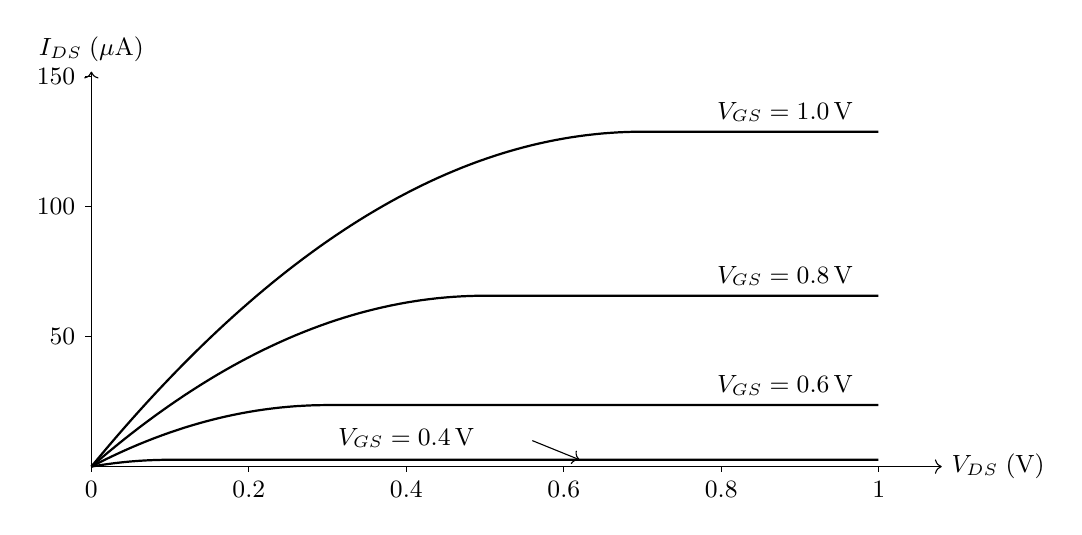
\begin{tikzpicture}[x=10cm,y=0.033cm,font=\small]
\draw[->] (0,0)--(1.08,0) node[right] {$V_{DS}\;(\mathrm V)$};
\draw[->] (0,0)--(0,152) node[above] {$I_{DS}\;(\mathrm{\mu A})$};
\foreach \x in {0,0.2,0.4,0.6,0.8,1}{\draw (\x,0)--(\x,-2) node[below] {$\x$};}
\foreach \y in {50,100,150}{\draw (0,\y)--(-0.008,\y) node[left] {$\y$};}
\foreach \g in {0.4,0.6,0.8,1.0}{
 \draw[thick,domain=0:1,samples=101] plot (\x,{526*((\g-0.3)*min(\x,\g-0.3)-0.5*min(\x,\g-0.3)^2)});
}
\node[anchor=south east] at (0.98,128.87) {$V_{GS}=1.0\,\mathrm V$};
\node[anchor=south east] at (0.98,65.75) {$V_{GS}=0.8\,\mathrm V$};
\node[anchor=south east] at (0.98,23.67) {$V_{GS}=0.6\,\mathrm V$};
\draw[->] (0.56,10)--(0.62,2.63);
\node at (0.40,11) {$V_{GS}=0.4\,\mathrm V$};
\end{tikzpicture}
\end{latin}
\caption{منحنی‌های مدل ایدئال مثال \secnum{۲.۱} کتاب با
\(\beta_n=\qty{526}{\micro\ampere\per\volt\squared}\).
دو منحنی \(V_{GS}=0\) و \(V_{GS}=\qty{0.2}{\volt}\) روی محور افقی قرار دارند
\cite[شکل \secnum{۲.۷}]{weste}.}
\label{fig:mos-book-curves}
\end{figure}

\subsection{\lr{pMOS} با بزرگی مثبت و سپس قرارداد علامت‌دار}
برای \lr{pMOS}، \lr{Source} پایانه پرپتانسیل‌تر است. آستانه علامت‌دار را
\(V_{tp}<0\) و بزرگی مثبت آن را \(V_{TP}=|V_{tp}|\) می‌نامیم.
ولتاژها و ضریب مثبت را به صورت زیر تعریف می‌کنیم
\begin{equation}
 V_{SG}=V_S-V_G,\quad V_{SD}=V_S-V_D,\quad
 V_{GT,p}=V_{SG}-V_{TP},\quad
 \beta_p=\mu_p C_{\mathrm{ox}}\frac{W_p}{L_p}>0.
 \label{eq:mos-p-defs}
\end{equation}
با این تعریف، برای \(V_{SD}\ge0\)، بزرگی جریان از \lr{Source} به \lr{Drain}
دقیقاً همان ساختار مدل \lr{nMOS} را دارد
\cite[صفحه ۶۷ و اسلایدهای ۲۱ و ۲۲]{weste,mos}.
\begin{equation}
 |I_{DS,p}|=\begin{cases}
 0,&V_{SG}\le V_{TP},\\[2pt]
 \beta_p(V_{GT,p}V_{SD}-V_{SD}^2/2),
 &V_{SG}>V_{TP},\quad 0\le V_{SD}<V_{GT,p},\\[2pt]
 \beta_p V_{GT,p}^2/2,
 &V_{SG}>V_{TP},\quad V_{SD}\ge V_{GT,p}.
 \end{cases}
 \label{eq:mos-p-piecewise}
\end{equation}
در قرارداد جریان \lr{Drain}-به-\lr{Source}، مقدار جریان \lr{pMOS} منفی است.
همچنین \(V_{GS}=-V_{SG}\) و \(V_{DS}=-V_{SD}\) هستند.
بنابراین نمودار علامت‌دار کتاب در ربع سوم قرار می‌گیرد.
برای نوشتن رابطه علامت‌دار اشباع با \(\beta_p>0\)، می‌توان نوشت
\begin{equation}
 I_{DS,p}=-\frac{\beta_p}{2}(V_{GS}-V_{tp})^2,
 \quad V_{GS}<V_{tp},\quad V_{SD}\ge V_{GT,p}.
 \label{eq:mos-p-signed}
\end{equation}
کتاب برای ساده‌کردن محاسبه‌ها اغلب بزرگی‌ها را به کار می‌برد.
در هر مسئله، قرارداد بزرگی یا علامت‌دار باید در تمام رابطه ثابت بماند.

مثال فرضی \(V_S=\qty{1.8}{\volt}\)، \(V_G=\qty{0.6}{\volt}\)،
\(V_D=\qty{1.5}{\volt}\)، \(V_{tp}=-\qty{0.4}{\volt}\) و
\(\beta_p=\qty{100}{\micro\ampere\per\volt\squared}\) را در نظر بگیرید.
\(V_{SG}=\qty{1.2}{\volt}\)، \(V_{GT,p}=\qty{0.8}{\volt}\) و
\(V_{SD}=\qty{0.3}{\volt}\) هستند. پس ناحیه \lr{Linear} و جریان
\[
 |I_{DS,p}|=100\left[0.8(0.3)-\frac{0.3^2}{2}\right]\,\unit{\micro\ampere}
 =\qty{19.5}{\micro\ampere}
\]
است. در قرارداد علامت‌دار، \(V_{DS}=-\qty{0.3}{\volt}\) و
\(I_{DS,p}=-\qty{19.5}{\micro\ampere}\) می‌شوند.
اگر تنها \(V_D\) به \qty{0.6}{\volt} کاهش یابد، \(V_{SD}=\qty{1.2}{\volt}\)
و ناحیه \lr{Saturation} است. بزرگی جریان
\((100/2)(0.8)^2=\qty{32}{\micro\ampere}\) خواهد بود.

در نمونه \lr{pMOS} همراه شکل \secnum{۲.۷} کتاب، هندسه و بزرگی آستانه با نمونه
\lr{nMOS} یکسان و \(\mu_p=\mu_n/2\) است. پس در ولتاژهای متناظر، بزرگی جریان
نصف می‌شود. مثلاً نقطه \((V_{DS},I_{DS})=(\qty{1}{\volt},\qty{128.87}{\micro\ampere})\)
در نمونه \lr{nMOS} متناظر با حدود
\((-\qty{1}{\volt},-\qty{64.44}{\micro\ampere})\) در نمونه \lr{pMOS} است.

\clearpage
\subsection{نسبت \lr{Mobility} و انتخاب عرض \lr{pMOS}}
برای دو ترانزیستور با \(L\)، \(C_{\mathrm{ox}}\) و اضافه‌ولتاژ یکسان، برابرشدن
جریان در مدل نیازمند \(\beta_p=\beta_n\) است. از \eqref{eq:mos-beta} داریم
\begin{equation}
 \mu_pW_p=\mu_nW_n
 \quad\Longrightarrow\quad
 \frac{W_p}{W_n}=\frac{\mu_n}{\mu_p}.
 \label{eq:mos-width-ratio}
\end{equation}
اسلاید ۲۲ مقادیر \(\mu_n=350\) و \(\mu_p=120\) را برای نمونه فناوری خود ذکر
می‌کند. نسبت این دو حدود \num{2.92} است. همان اسلاید برای مثال‌های کلاس، نسبت ۲ را
به عنوان فرض قراردادی اعلام می‌کند. کتاب نیز نسبت متداول ۲ تا ۳ را بیان کرده و
برای مثال‌هایش معمولاً ۲ می‌گیرد. پس با داده عددی ۳۵۰ و ۱۲۰، عرض حدود \num{2.92} برابر
و با فرض قراردادی ۲، عرض دو برابر به دست می‌آید.
\(\mu\)های این پاراگراف واحد مشترک
\unit{\centi\metre\squared\per\volt\per\second} دارند.

اگر طول یا ظرفیت اکسید یا اضافه‌ولتاژها برابر نباشند، باید از خود رابطه جریان
استفاده کرد. برای اشباع و اضافه‌ولتاژهای مثبت، برابرشدن جریان‌ها می‌دهد
\begin{equation}
 \frac{W_p}{W_n}
 =\frac{\mu_nC_{\mathrm{ox},n}}{\mu_pC_{\mathrm{ox},p}}
 \frac{L_p}{L_n}\left(\frac{V_{GT,n}}{V_{GT,p}}\right)^2.
 \label{eq:mos-general-width}
\end{equation}
بنابراین نسبت عرض از فرض‌های فیزیکی و نقطه بایاس مسئله نتیجه می‌شود.
\clearpage

\subsection{تحلیل مدار مقاومتی و انتخاب ریشه فیزیکی}
در مدار شکل \ref{fig:mos-load}، \lr{Source} و \lr{Body} به زمین،
\lr{Drain} از طریق \(R_D\) به \(V_{DD}\) و \lr{Gate} به ولتاژ ثابت \(V_G\)
متصل‌اند. برای مثال آموزشی، \(V_{DD}=\qty{1.8}{\volt}\)،
\(V_G=\qty{1.2}{\volt}\)، \(V_{tn}=\qty{0.4}{\volt}\) و
\(\beta_n=\qty{1}{\milli\ampere\per\volt\squared}\) هستند.
\begin{figure}[ht]
\centering
\begin{latin}
\begin{circuitikz}[font=\small]
\draw (0,0) node[nmos] (M) {};
\draw (M.S)--++(0,-0.4) node[ground] {};
\draw (M.D) to[R,l=$R_D$] ++(0,2) node[vcc] {$V_{DD}$};
\draw (M.G)--++(-1,0) node[ocirc] {} node[left] {$V_G$};
\draw (M.D)--++(1,0) node[ocirc] {} node[right] {$V_D=V_{DS}$};
\end{circuitikz}
\end{latin}
\caption{مدار آموزشی برای پیوند رابطه ترانزیستور با قانون جریان و ولتاژ مدار.
اتصال \lr{Body} به زمین در نماد به صورت ضمنی فرض شده است.}
\label{fig:mos-load}
\end{figure}

ابتدا اضافه‌ولتاژ گیت را محاسبه می‌کنیم.
\[
 V_{GT}=1.2-0.4=\qty{0.8}{\volt}.
\]
از افت ولتاژ مقاومت و برابری جریان مقاومت با جریان ترانزیستور داریم
\begin{equation}
 I_{DS}=\frac{V_{DD}-V_D}{R_D}.
 \label{eq:mos-load-line}
\end{equation}
برای \(R_D=\qty{2}{\kilo\ohm}\)، ابتدا اشباع را فرض می‌کنیم.
جریان پیشنهادی و ولتاژ متناظر با آن چنین‌اند.
\[
 \begin{aligned}
 I_{DS}&=(1/2)(0.8)^2=\qty{0.32}{\milli\ampere},\\
 V_D&=1.8-(0.32)(2)=\qty{1.16}{\volt}.
 \end{aligned}
\]
در این ضرب، \unit{\milli\ampere} در \unit{\kilo\ohm} واحد \unit{\volt} می‌دهد.
چون \(1.16\ge0.8\)، شرط اشباع برقرار و فرض تأیید می‌شود.

اکنون \(R_D=\qty{5}{\kilo\ohm}\) را بگذارید. فرض اشباع همان جریان
\qty{0.32}{\milli\ampere} را می‌دهد. ولتاژ متناظر با این فرض برابر است با
\[
 V_D=1.8-(0.32)(5)=\qty{0.2}{\volt}.
\]
چون \(0.2<0.8\)، این فرض با شرط ناحیه سازگار نیست.
با فرض \lr{Linear} و نوشتن جریان در \unit{\milli\ampere} و ولتاژ در \unit{\volt}،
رابطه مقاومت و ترانزیستور را برابر می‌کنیم
\begin{align}
 \frac{1.8-V_D}{5}&=0.8V_D-\frac{V_D^2}{2},\notag\\
 0.36-0.2V_D&=0.8V_D-0.5V_D^2,\notag\\
 0.5V_D^2-V_D+0.36&=0.
 \label{eq:mos-load-quadratic}
\end{align}
اعداد رابطه \eqref{eq:mos-load-quadratic} در دستگاه واحد معرفی‌شده نوشته شده‌اند.
برای معادله \(aV_D^2+bV_D+c=0\)، فرمول ریشه
به صورت زیر است.
\[
 V_D=\frac{-b\pm\sqrt{b^2-4ac}}{2a}.
\]
با \(a=0.5,b=-1,c=0.36\)، داخل رادیکال \(1-0.72=0.28\) می‌شود، پس
\begin{equation*}
 V_D=1\pm\sqrt{0.28},\qquad
 V_{D,1}\approx\qty{0.471}{\volt},\qquad
 V_{D,2}\approx\qty{1.529}{\volt}.
\end{equation*}
شرط ناحیه انتخاب‌شده \(0\le V_D<\qty{0.8}{\volt}\) است.
فقط ریشه \qty{0.471}{\volt} این شرط را دارد. ریشه دوم از ادامه ریاضی رابطه
\lr{Linear} به بیرون بازه معتبر آن به دست آمده است. با ریشه پذیرفته‌شده،
جریان چنین محاسبه می‌شود.
\[
 I_{DS}=\frac{1.8-0.47085}{5}\approx\qty{0.266}{\milli\ampere}.
\]
جای‌گذاری در رابطه ترانزیستور نیز همین جریان را می‌دهد.

\subsection{تمرین‌های پاسخ‌دار و مرور تحلیلی}
\textbf{تمرین ۱.} با \(V_G=\qty{0.8}{\volt}\)، \(V_S=\qty{0.5}{\volt}\)،
\(V_D=\qty{1.2}{\volt}\) و آستانه ثابت \qty{0.4}{\volt}، جریان مدل چیست؟
\(V_{GS}=0.8-0.5=\qty{0.3}{\volt}\) و کمتر از آستانه است.
پس در مدل مرتبه اول \(I_{DS}=0\)، هرچند ولتاژ \lr{Drain} مثبت است.

\textbf{تمرین ۲.} برای \(\beta_n=\qty{200}{\micro\ampere\per\volt\squared}\)،
\(V_{tn}=\qty{0.4}{\volt}\)، \(V_{GS}=\qty{1.2}{\volt}\) و
\(V_{DS}=\qty{0.2}{\volt}\)، ناحیه و جریان را بیابید.
\(V_{GT}=\qty{0.8}{\volt}\) و \(0.2<0.8\)، پس \lr{Linear} است.
جریان از رابطه \lr{Linear} به دست می‌آید.
\[
 200[0.8(0.2)-0.2^2/2]=\qty{28}{\micro\ampere}.
\]

\textbf{تمرین ۳.} در تمرین قبل، \(V_{DS}=\qty{1}{\volt}\) شود.
اکنون \(1\ge0.8\)، پس اشباع برقرار است. جریان برابر است با
\[
 I_{DS}=(200/2)(0.8)^2=\qty{64}{\micro\ampere}.
\]
اگر اشتباهاً رابطه \lr{Linear} را ادامه دهیم، \qty{60}{\micro\ampere} می‌دهد.
این عدد شرط اعتبار همان فرمول را نقض می‌کند.

\textbf{تمرین ۴.} در اشباع، \(I_{DS}=\qty{36}{\micro\ampere}\)،
\(\beta_n=\qty{200}{\micro\ampere\per\volt\squared}\) و
\(V_{tn}=\qty{0.4}{\volt}\) است. \(V_{GS}\) را بیابید.
ابتدا مربع اضافه‌ولتاژ را از رابطه جریان جدا می‌کنیم.
\[
 (V_{GS}-0.4)^2=\frac{2(36)}{200}=0.36\,\unit{\volt\squared}.
\]
ریشه‌ها \(V_{GS}=0.4\pm0.6\) هستند.
شرط \(V_{GS}>V_{tn}\)، پاسخ \(V_{GS}=\qty{1}{\volt}\) را انتخاب می‌کند.
برای معتبرماندن فرض اشباع، \(V_{DS}\ge\qty{0.6}{\volt}\) نیز لازم است.

\textbf{تمرین ۵.} در فرض اشباع، \(V_{tn}=\qty{0.3}{\volt}\) و سایر پارامترها
ثابت باشند. کاهش \(V_{GS}\) از \qty{1}{\volt} به \qty{0.8}{\volt}
جریان را در چه نسبتی تغییر می‌دهد؟
اضافه‌ولتاژها \qty{0.7}{\volt} و \qty{0.5}{\volt} هستند، بنابراین
\[
 \frac{I_2}{I_1}=\frac{(0.8-0.3)^2}{(1-0.3)^2}
 =\frac{0.25}{0.49}\approx0.510.
\]
جریان حدود ۴۹ درصد کاهش می‌یابد. مربعِ نسبت اضافه‌ولتاژها در رابطه ظاهر می‌شود.

\textbf{تمرین ۶.} اگر \(W\) و \(L\) هر دو دو برابر شوند، با سایر شرایط ثابت،
جریان این مدل چه تغییری می‌کند؟ نسبت \(W/L\) ثابت و در نتیجه \(\beta\)
و جریان ثابت می‌مانند. مدل صفحه‌ای، \(C_g\propto WL\)، ظرفیت را چهار برابر می‌دهد.
برای استنباط تأخیر مدار باید اثر بار و جریان همه مراحل بررسی شود.

\textbf{تمرین ۷.} با \(\mu_n/\mu_p=2\)، طول برابر، اکسید برابر و بزرگی آستانه
برابر، جریان متناظر \lr{pMOS} با عرض برابر نسبت به \lr{nMOS} چقدر است؟
\(\beta_p/\beta_n=1/2\)، پس در اضافه‌ولتاژ و ناحیه متناظر، بزرگی جریان نصف است.
عرض دو برابر \lr{pMOS}، ضریب‌ها را در همین فرض‌ها برابر می‌کند.

\textbf{تمرین ۸.} برای \lr{pMOS} با \(V_S=\qty{1.2}{\volt}\)،
\(V_G=\qty{1.0}{\volt}\)، \(V_D=\qty{0.2}{\volt}\) و
\(V_{tp}=-\qty{0.3}{\volt}\)، ناحیه چیست؟
\(V_{SG}=\qty{0.2}{\volt}<|V_{tp}|\)، پس \lr{Cutoff} است.
بزرگی زیاد \(V_{SD}\) شرط روشن‌شدن را تأمین نمی‌کند.

\textbf{تمرین ۹.} در مثال اسلاید، با \(\beta_n=\qty{240}{\micro\ampere\per\volt\squared}\)،
\(V_{GS}=\qty{5}{\volt}\) و \(V_{DS}=\qty{5}{\volt}\)، جریان و ناحیه را بیابید.
اضافه‌ولتاژ گیت برابر است با
\[
 V_{GT}=5-0.7=\qty{4.3}{\volt}.
\]
پس اشباع برقرار است و محاسبه جریان می‌دهد
\[
 (240/2)(4.3)^2=\qty{2218.8}{\micro\ampere}\approx\qty{2.22}{\milli\ampere}.
\]
این نتیجه با منحنی بالای شکل \ref{fig:mos-slide-curves} سازگار است.

\textbf{تمرین ۱۰.} چرا در مرز \(V_{DS}=V_{GT}\) دو فرمول جریان برابرند؟
در قطعه \lr{Linear}، جای‌گذاری می‌دهد
\[
 \beta_n(V_{GT}^2-V_{GT}^2/2)=\beta_nV_{GT}^2/2.
\]
این دقیقاً مقدار قطعه اشباع است. بنابراین نحوه نسبت‌دادن خود نقطه مرزی به یکی
از دو ناحیه، مقدار جریان را تغییر نمی‌دهد.

در حل مسئله، مسیر محاسبه از تعریف اختلاف ولتاژ آغاز می‌شود، سپس شرط روشن‌شدن،
مرز ناحیه و مقدار جریان بررسی می‌شوند. اگر ولتاژ یا جریان مجهول از معادله مدار
به دست آید، نتیجه باید دوباره در شرط ناحیه جای‌گذاری شود.
این روند، ریشه ریاضی را به پاسخ سازگار با مدل فیزیکی تبدیل می‌کند.
\clearpage

\section{مشخصه‌های ظرفیت و ولتاژ، \lr{C-V}}
\label{sec:book-cv}
در مدل تفصیلی این بخش، پسوند \(i\) سهم \lr{Intrinsic} و پسوند
\(\mathrm{ov}\) سهم \lr{Overlap} را مشخص می‌کند.
\(C_0=WLC_{\mathrm{ox}}\) ظرفیت هندسی مرجع است.
نماد بدون این پسوندها، در مدار معادل کامل، مجموع سهم‌های دو پایانه مربوط را
نشان می‌دهد. ظرفیت مؤثر گذار، علاوه بر بایاس به حرکت پایانه دیگر نیز وابسته است.
\BookletSubsections{notes/booklet-01/ch2-capacitance-basics}
\BookletSubsections{notes/booklet-01/ch2-gate-capacitance}
\BookletSubsections{notes/booklet-01/ch2-diffusion-capacitance}
\BookletReview{notes/booklet-01/final-review}


% !TeX root = booklet-02.tex
\BookletReview{notes/booklet-02/prerequisites}
\ifCompleteNotes\else
\setcounter{chapter}{1}
\chapter{اثرهای غیرایده‌آل جریان ترانزیستور}
\fi
\setcounter{section}{3}
\section{اثرهای غیرایده‌آل در مشخصه \lr{I-V}}
\label{sec:nonideal-current}
مدل \lr{Long-channel} نقطه شروع تحلیل است. در افزاره‌های با میدان قوی،
وابستگی سرعت به میدان و تغییر طول مؤثر کانال، شکل منحنی جریان را تغییر
می‌دهند. شکل \secnum{۲.۱۴} کتاب تفاوت جریان مدل ایده‌آل و مدل شبیه‌سازی‌شده
مرجع را نشان می‌دهد \cite[صفحه چاپی ۷۴]{weste}. در ادامه، منشأ اثرهای
میدان، طول مؤثر و آستانه، روابط تقریبی و روش استفاده سازگار از مدل‌ها را
بررسی می‌کنیم.
% !TeX root = booklet-02.tex
\subsection{\lr{Mobility Degradation} و \lr{Velocity Saturation}}
\label{sec:high-field}
\subsubsection*{دو میدان با دو نقش فیزیکی}
میدان عمودی، حامل‌های متحرک را نزدیک فصل مشترک \lr{Silicon} و اکسید
نگه می‌دارد. افزایش این میدان، پراکندگی حامل‌ها در نزدیکی فصل مشترک را
شدیدتر می‌کند و \lr{Mobility} مؤثر کاهش می‌یابد. میدان طولی در امتداد کانال،
حرکت رانشی ایجاد می‌کند. در میدان طولی بزرگ، سرعت با افزایش میدان به یک
حد نزدیک می‌شود. این دو پدیده در کتاب و اسلایدها به‌ترتیب
\lr{Mobility Degradation} و \lr{Velocity Saturation} نامیده شده‌اند
\cite[صفحات چاپی ۷۴ تا ۷۶]{weste}\cite[اسلایدهای ۶ تا ۹]{nonideal}.

برای برآورد مرتبه بزرگی، اسلاید ۶ از دو رابطه استفاده می‌کند
\begin{equation}
 E_{\mathrm{vert}}\sim\frac{V_{GS}}{t_{\mathrm{ox}}},\qquad
 \overline E_{\mathrm{lat}}=\frac{V_{DS}}{L}.
 \label{eq:fields-estimate}
\end{equation}
رابطه اول نمایش تقریبی وابستگی میدان عمودی به بایاس و ضخامت است.
افت واقعی ولتاژ اکسید و میدان مؤثر حامل‌ها به ساختار و توزیع بار وابسته‌اند.
رابطه دوم، میانگین میدان طولی روی طول کانال را می‌دهد. در استخراج رابطه
جریان، میدان محلی \(E(x)\) را دنبال می‌کنیم.

\subsubsection*{مدل تجربی کاهش \lr{Mobility}}
در رابطه \secnum{۲.۲۳} کتاب و اسلاید ۸، \lr{Mobility} مؤثر با یک مدل تجربی
برحسب بایاس گیت و ضخامت اکسید نوشته شده است. برای \lr{nMOS} و
\lr{pMOS}، روابط را با قرارداد بزرگی مثبت ولتاژها چنین بازنویسی می‌کنیم
\begin{align}
 \mu_{\mathrm{eff},n}
 &=\frac{\qty{540}{\centi\metre\squared\per\volt\per\second}}
 {1+\left[\dfrac{V_{GS}+V_{tn}}
 {\bigl(\qty{0.54}{\volt\per\nano\metre}\bigr)t_{\mathrm{ox}}}\right]^{1.85}},
 \label{eq:mobility-n}\\[3pt]
 \mu_{\mathrm{eff},p}
 &=\frac{\qty{185}{\centi\metre\squared\per\volt\per\second}}
 {1+\dfrac{\left|V_{SG}+1.5V_{TP}\right|}
 {\bigl(\qty{0.338}{\volt\per\nano\metre}\bigr)t_{\mathrm{ox}}}}.
 \label{eq:mobility-p}
\end{align}
در \eqref{eq:mobility-p}، \(V_{TP}=|V_{tp}|\) است. کتاب در این رابطه،
ولتاژهای \lr{pMOS} را به‌صورت بزرگی مثبت به کار می‌برد
\cite[رابطه \secnum{۲.۲۳} و مثال \secnum{۲.۳}]{weste}. صورت هر کسر،
مقیاس \lr{Mobility} در همان مدل تجربی است. اعداد ۵۴۰ و ۱۸۵ به همراه
واحدشان پارامترهای مدل‌اند. این ضرایب از برازش داده‌های افزاره به دست آمده‌اند.

در مخرج \eqref{eq:mobility-n}، ضریب
\(\qty{0.54}{\volt\per\nano\metre}\) در ضخامت ضرب می‌شود و نتیجه ولتاژ
است. نسبت دو ولتاژ بی‌بعد است و توان \(1.85\) به همین نسبت اعمال می‌شود.
اگر ضخامت را با واحد \(\unit{\nano\metre}\) وارد می‌کنیم، مقدار عددی
\(1.05\) برای ضخامت \(\qty{1.05}{\nano\metre}\) به کار می‌رود.
برای محاسبه کاملاً \lr{SI}، ضریب متناظر
\(\qty{5.4e8}{\volt\per\metre}\) است.

با ثابت بودن آستانه و ضخامت، افزایش \(V_{GS}\) در دامنه هدایت
\lr{nMOS}، مخرج \eqref{eq:mobility-n} را بزرگ‌تر و \(\mu_{\mathrm{eff},n}\)
را کوچک‌تر می‌کند. این نتیجه، کاهش \lr{Mobility} در مدل را نشان می‌دهد.
جریان هم‌زمان به مقدار بار کانال وابسته است و افزایش گیت می‌تواند با وجود
کاهش \lr{Mobility}، جریان را افزایش دهد. سهم هر عامل باید در رابطه کامل
جریان بررسی شود.

\subsubsection*{حل مرحله‌به‌مرحله مثال \secnum{۲.۳} کتاب}
مثال کتاب از \(V_{GS}=V_{SG}=\qty{1.0}{\volt}\)،
\(V_{tn}=V_{TP}=\qty{0.3}{\volt}\) و
\(t_{\mathrm{ox}}=\qty{1.05}{\nano\metre}\) استفاده می‌کند
\cite[صفحه چاپی ۷۶]{weste}. ابتدا بخش بی‌بعد مخرج را حساب می‌کنیم
\begin{align}
 a_n&=\frac{1.0+0.3}{0.54\times1.05}\approx2.293,
 &a_n^{1.85}&\approx4.642,\notag\\
 a_p&=\frac{1.0+1.5(0.3)}{0.338\times1.05}\approx4.086.
 \label{eq:mobility-example-ratios}
\end{align}
جایگذاری این اعداد در دو رابطه \lr{Mobility} نتیجه می‌دهد
\begin{align}
 \mu_{\mathrm{eff},n}
 &\approx\frac{540}{1+4.642}
 \approx\qty{95.7}{\centi\metre\squared\per\volt\per\second},\notag\\
 \mu_{\mathrm{eff},p}
 &\approx\frac{185}{1+4.086}
 \approx\qty{36.4}{\centi\metre\squared\per\volt\per\second}.
 \label{eq:mobility-example-results}
\end{align}
اعداد گرد‌شده کتاب، به‌ترتیب ۹۶ و ۳۶ با واحد
\(\unit{\centi\metre\squared\per\volt\per\second}\) هستند. در مثال
ولتاژ بحرانی از همین گردکردن استفاده می‌کنیم. برای محاسبات چندمرحله‌ای،
نگهداری رقم‌های بیشتر تا انتهای محاسبه خطای گردکردن را محدود می‌کند.

مثال \secnum{۲.۱} کتاب برای مدل ایده‌آل یک مقدار ثابت
\(\qty{80}{\centi\metre\squared\per\volt\per\second}\) به \lr{Mobility}
الکترون نسبت می‌دهد. رابطه تجربی \eqref{eq:mobility-n} مجموعه پارامترهای
دیگری دارد. برای مقایسه کنترل‌شده اثر \lr{Velocity Saturation} در این جزوه،
\lr{Mobility} مؤثر را در دو محاسبه یکسان می‌گیریم. تفسیر کاهش \lr{Mobility}
در \eqref{eq:mobility-n} بر اساس صورت ۵۴۰ و وابستگی به بایاس همان مدل
انجام می‌شود \cite[مثال‌های \secnum{۲.۱} و \secnum{۲.۳}]{weste}.

\subsubsection*{مدل سرعت و دلیل ضریب دو در میدان بحرانی}
در میدان کوچک، سرعت رانش با میدان متناسب است و \(v=\mu_{\mathrm{eff}}E\).
در میدان بزرگ، سرعت متوسط به \(v_{\mathrm{sat}}\) نزدیک می‌شود. مدل قطعه‌ای
کتاب این رفتار را چنین تقریب می‌زند
\cite[روابط \secnum{۲.۲۴} و \secnum{۲.۲۵}]{weste}\cite[اسلاید ۹]{nonideal}
\begin{equation}
 v(E)=\begin{cases}
 \dfrac{\mu_{\mathrm{eff}}E}{1+E/E_c},&0\le E<E_c,\\[5pt]
 v_{\mathrm{sat}},&E\ge E_c.
 \end{cases}
 \label{eq:velocity-model}
\end{equation}
نماد \(E_c\) میدان بحرانی است. در مرز \(E=E_c\)، حد شاخه اول برابر
\(\mu_{\mathrm{eff}}E_c/2\) است. برای پیوستگی سرعت، این مقدار باید با
\(v_{\mathrm{sat}}\) برابر باشد. ازاین‌رو
\begin{equation}
 \frac{\mu_{\mathrm{eff}}E_c}{2}=v_{\mathrm{sat}}
 \quad\Longrightarrow\quad
 \boxed{E_c=\frac{2v_{\mathrm{sat}}}{\mu_{\mathrm{eff}}}}.
 \label{eq:critical-field}
\end{equation}
ضریب دو از شکل مشخص شاخه اول در \eqref{eq:velocity-model} به دست آمده است.
برای \(E\ll E_c\)، مخرج تقریباً یک است و قانون میدان کوچک بازیابی می‌شود.
نمودار بی‌بعد شکل \ref{fig:velocity-normalized} همین اتصال دو شاخه را نشان
می‌دهد. با تعریف \(u=E/E_c\)، شاخه اول برابر
\(v/v_{\mathrm{sat}}=2u/(1+u)\) می‌شود.

\begin{figure}[!htbp]
\centering
\begin{latin}
\PersianMathDigits
\begin{tikzpicture}[x=3.2cm,y=2.5cm]
 \draw[->] (0,0)--(2.15,0) node[right] {\(E/E_c\)};
 \draw[->] (0,0)--(0,2.15) node[above] {\(v/v_{\mathrm{sat}}\)};
 \draw[densely dashed,gray] (0,0)--(1,2) node[above right] {\(v=\mu_{\mathrm{eff}}E\)};
 \draw[thick,domain=0:1,samples=70] plot (\x,{2*\x/(1+\x)});
 \draw[thick] (1,1)--(2,1);
 \draw[dotted] (1,0)--(1,1)--(0,1);
 \foreach \x in {0,1,2} {\draw (\x,0)--(\x,-0.03) node[below] {\(\x\)};}
 \foreach \y in {1,2} {\draw (0,\y)--(-0.03,\y) node[left] {\(\y\)};}
\end{tikzpicture}
\end{latin}
\caption{نمودار آموزشی مدل سرعت \eqref{eq:velocity-model}. خط‌چین امتداد قانون میدان کوچک و خط پیوسته مدل قطعه‌ای کتاب را نشان می‌دهد.}
\label{fig:velocity-normalized}
\end{figure}

در کتاب، \(v_{\mathrm{sat},n}\approx\qty{e7}{\centi\metre\per\second}\)
و \(v_{\mathrm{sat},p}\approx\qty{8e6}{\centi\metre\per\second}\) ذکر
شده‌اند \cite[صفحه چاپی ۷۶]{weste}. این مقادیر و ضرایب \lr{Mobility}،
پارامترهای مدل مورد استفاده مرجع‌اند. در اسلاید ۹، استقلال \(E_c\) از
\(V_{DS}\) و \(L\) در مدل بیان شده است. با ثابت بودن بایاس گیت و پارامترهای
ماده، \eqref{eq:critical-field} نیز همین رفتار را دارد. هنگام تغییر
\(V_{GS}\)، \(\mu_{\mathrm{eff}}\) می‌تواند تغییر کند و مقدار \(E_c\)
باید سازگار با آن به‌روزرسانی شود.

\subsubsection*{ولتاژ بحرانی و حل مثال \secnum{۲.۴}}
ولتاژ بحرانی را با استفاده از طول کانال تعریف می‌کنیم
\begin{equation}
 V_c=E_cL=\frac{2v_{\mathrm{sat}}L}{\mu_{\mathrm{eff}}}.
 \label{eq:critical-voltage}
\end{equation}
واحد \(E_cL\) برابر ولت است. در مثال کتاب، \(L=\qty{50}{\nano\metre}
=\qty{5e-6}{\centi\metre}\) است. جایگذاری مقادیر گرد‌شده
\eqref{eq:mobility-example-results} می‌دهد
\begin{align}
 E_{c,n}&=\frac{2\times10^7}{96}
 \approx\qty{2.08e5}{\volt\per\centi\metre},
 &V_{c,n}&\approx(2.08\times10^5)(5\times10^{-6})\,\unit{\volt}
 \approx\qty{1.04}{\volt},\notag\\
 E_{c,p}&=\frac{2(8\times10^6)}{36}
 \approx\qty{4.44e5}{\volt\per\centi\metre},
 &V_{c,p}&\approx\qty{2.22}{\volt}.
 \label{eq:critical-example}
\end{align}
این نتایج با مثال \secnum{۲.۴} کتاب و اسلاید ۱۲ تطبیق دارند
\cite{weste,nonideal}. در این نمونه، \(V_c\) در \lr{pMOS} بزرگ‌تر است و
برای اضافه‌ولتاژ گیت یکسان، اثر محدودشدن سرعت ضعیف‌تر خواهد بود. نسبت
\(V_{GT}/V_c\) در جریان استخراج‌شده این تفاوت را کمّی می‌کند.

تعریف \(V_c\) با میدان متوسط، مقیاسی برای مقایسه بایاس‌هاست. میدان محلی
نزدیک \lr{Drain} می‌تواند زودتر از میدان متوسط به \(E_c\) برسد.
ولتاژ شروع اشباع جریان، \(V_{\mathrm{dsat}}\)، در ادامه از شرط مرزی همان
مدل تعیین می‌شود.

\subsubsection*{استخراج رابطه جریان با میدان محلی}
محور \(x\) را از \lr{Source} به \lr{Drain} می‌گیریم و \(V(x)\) را
پتانسیل کانال نسبت به \lr{Source} تعریف می‌کنیم. کران‌ها
\(V(0)=0\) و \(V(L)=V_{DS}\) هستند. برای اختصار،
\(A=V_{GT}>0\) و \(D=V_{DS}\) می‌گذاریم. بزرگی بار متحرک بر واحد
طول کانال در مدل تدریجی برابر است با
\begin{equation}
 q'(x)=WC_{\mathrm{ox}}[A-V(x)].
 \label{eq:local-charge}
\end{equation}
این بیان بار، همان مبنای بخش \secnum{۲.۲} کتاب است. تغییر این استخراج،
استفاده از رابطه سرعت \eqref{eq:velocity-model} است
\cite[بخش‌های \secnum{۲.۲} و \secnum{۲.۴.۱}]{weste}.

پیش از رسیدن میدان انتهای کانال به \(E_c\)، با
\(E(x)=\mathrm{d}V/\mathrm{d}x\)، جریان در هر مقطع چنین نوشته می‌شود
\begin{equation}
 I=WC_{\mathrm{ox}}(A-V)
 \frac{\mu_{\mathrm{eff}}\,\mathrm{d}V/\mathrm{d}x}
 {1+(\mathrm{d}V/\mathrm{d}x)/E_c}.
 \label{eq:current-local}
\end{equation}
در محاسبه برای یک بایاس گیت ثابت، \(\mu_{\mathrm{eff}}\) را در طول کانال
ثابت می‌گیریم. جریان \lr{DC} نیز در همه مقاطع یکسان است. ابتدا دو طرف را
در مخرج و سپس در \(\mathrm{d}x\) ضرب می‌کنیم
\begin{align}
 I+\frac{I}{E_c}\frac{\mathrm{d}V}{\mathrm{d}x}
 &=\mu_{\mathrm{eff}}WC_{\mathrm{ox}}(A-V)
 \frac{\mathrm{d}V}{\mathrm{d}x},\notag\\
 I\,\mathrm{d}x
 &=\left[\mu_{\mathrm{eff}}WC_{\mathrm{ox}}(A-V)-\frac{I}{E_c}\right]
 \mathrm{d}V.
 \label{eq:current-separated}
\end{align}
اکنون سمت چپ روی طول کانال و سمت راست روی اختلاف پتانسیل جمع می‌شود.
با استفاده از انتگرال‌های مرور پیش‌نیاز داریم
\begin{align}
 IL&=\mu_{\mathrm{eff}}WC_{\mathrm{ox}}
 \int_0^D(A-V)\,\mathrm{d}V-\frac{I}{E_c}\int_0^D\mathrm{d}V,\notag\\
 IL&=\mu_{\mathrm{eff}}WC_{\mathrm{ox}}\left(AD-\frac{D^2}{2}\right)
 -\frac{ID}{E_c},\notag\\
 I\left(L+\frac{D}{E_c}\right)
 &=\mu_{\mathrm{eff}}WC_{\mathrm{ox}}\left(AD-\frac{D^2}{2}\right).
 \label{eq:current-integrated}
\end{align}
با تقسیم بر \(L\)، استفاده از \(E_cL=V_c\) و تعریف
\(\beta_{\mathrm{eff}}=\mu_{\mathrm{eff}}C_{\mathrm{ox}}W/L\)، نتیجه می‌شود
\begin{equation}
 \boxed{I_{\mathrm{lin}}=
 \frac{\beta_{\mathrm{eff}}\left(V_{GT}V_{DS}-V_{DS}^2/2\right)}
 {1+V_{DS}/V_c}},\qquad 0\le V_{DS}<V_{\mathrm{dsat}}.
 \label{eq:high-field-linear}
\end{equation}
این رابطه با شاخه نخست رابطه \secnum{۲.۲۶} کتاب برابر است. مخرج بی‌بعد،
اثر کاهش سرعت نسبت به قانون میدان کوچک را در جریان وارد می‌کند. اگر
\(V_{DS}/V_c\) کوچک باشد، مخرج به یک نزدیک می‌شود.

\subsubsection*{شرط انتهای کانال و اثبات تمرین \secnum{۲.۶}}
تمرین \secnum{۲.۶}، اثبات رابطه \secnum{۲.۲۷} کتاب را می‌خواهد
\cite[صفحه چاپی ۹۶]{weste}. در مرز اشباع این مدل، میدان محلی انتهای کانال
به \(E_c\) و سرعت به \(v_{\mathrm{sat}}\) می‌رسد. اگر
\(s=V_{\mathrm{dsat}}\) باشد، رابطه \eqref{eq:local-charge} بار بر واحد
طول انتهای کانال را برابر \(WC_{\mathrm{ox}}(A-s)\) می‌دهد. بنابراین
\begin{equation}
 I_{\mathrm{sat}}=WC_{\mathrm{ox}}(A-s)v_{\mathrm{sat}}.
 \label{eq:drain-saturation-current}
\end{equation}
در این مدل، برای \(V_{DS}\ge s\)، افزایش بایاس \lr{Drain} با ناحیه
میدان قوی انتهای کانال همراه است و جریان را به همین مقدار محدود می‌کنیم
\cite[رابطه \secnum{۲.۲۶}]{weste}.

در مرز، دو شاخه باید یک جریان بدهند. از \eqref{eq:critical-voltage}،
\(v_{\mathrm{sat}}=\mu_{\mathrm{eff}}V_c/(2L)\) است. جایگذاری می‌دهد
\begin{equation}
 \frac{\mu_{\mathrm{eff}}WC_{\mathrm{ox}}}{L}
 \frac{(A-s/2)s}{1+s/V_c}
 =WC_{\mathrm{ox}}(A-s)\frac{\mu_{\mathrm{eff}}V_c}{2L}.
 \label{eq:boundary-equality}
\end{equation}
عامل \(\mu_{\mathrm{eff}}WC_{\mathrm{ox}}/L\) در دو طرف مثبت و مشترک است.
آن را حذف می‌کنیم و دو طرف را در \(2(1+s/V_c)\) ضرب می‌کنیم
\begin{align}
 2(A-s/2)s&=(A-s)(V_c+s),\notag\\
 2As-s^2&=AV_c+As-V_cs-s^2,\notag\\
 As+V_cs&=AV_c,\notag\\
 (A+V_c)s&=AV_c.
 \label{eq:saturation-algebra}
\end{align}
جمله‌های \(-s^2\) از دو طرف حذف می‌شوند. چون \(A+V_c>0\)، تقسیم بر آن
مجاز است و جواب یکتا به دست می‌آید
\begin{equation}
 \boxed{V_{\mathrm{dsat}}=\frac{V_{GT}V_c}{V_{GT}+V_c}}.
 \label{eq:high-field-saturation-voltage}
\end{equation}
صورت، واحد ولت به توان دو و مخرج، واحد ولت دارد. پس جواب ولتاژ است.
برای \(V_{GT}>0,V_c>0\)، دو نسبت زیر را می‌نویسیم
\begin{equation}
 \frac{V_{\mathrm{dsat}}}{V_{GT}}=\frac{V_c}{V_{GT}+V_c}<1,\qquad
 \frac{V_{\mathrm{dsat}}}{V_c}=\frac{V_{GT}}{V_{GT}+V_c}<1.
 \label{eq:saturation-bounds}
\end{equation}
در نتیجه، \(0<V_{\mathrm{dsat}}<\min(V_{GT},V_c)\) و بار انتهای کانال
در مرز مثبت است. شکل جبری \(ab/(a+b)\) در فرمول دو مقاومت موازی نیز
دیده می‌شود. در اینجا دو عامل \(V_{GT},V_c\) هر دو ولتاژند.

با جایگذاری \eqref{eq:high-field-saturation-voltage} در
\eqref{eq:drain-saturation-current}، ابتدا اختلاف \(A-s\) را ساده می‌کنیم
\[
 A-s=A-\frac{AV_c}{A+V_c}=\frac{A^2}{A+V_c}.
\]
بنابراین جریان اشباع به شکل زیر نوشته می‌شود
\begin{equation}
 \boxed{I_{\mathrm{sat}}
 =WC_{\mathrm{ox}}v_{\mathrm{sat}}\frac{V_{GT}^2}{V_{GT}+V_c}}.
 \label{eq:high-field-saturation-current}
\end{equation}
این نتیجه همان رابطه \secnum{۲.۲۸} کتاب است. ضرب
\(WC_{\mathrm{ox}}\) در یک ولتاژ و یک سرعت، واحد آمپر می‌دهد.

\subsubsection*{حدهای مدل و تفاوت دو معنای \lr{Saturation}}
برای آشکارشدن حد کانال بلند، از \(v_{\mathrm{sat}}=
\mu_{\mathrm{eff}}V_c/(2L)\) استفاده می‌کنیم
\begin{equation}
 I_{\mathrm{sat}}=
 \frac{\beta_{\mathrm{eff}}V_{GT}^2}{2}
 \frac{1}{1+V_{GT}/V_c}.
 \label{eq:current-reduction-factor}
\end{equation}
اگر \(V_{GT}\ll V_c\)، عامل آخر به یک و
\(V_{\mathrm{dsat}}\) به \(V_{GT}\) نزدیک می‌شود. جریان مربعی مدل
\lr{Long-channel} با همان \lr{Mobility} مؤثر به دست می‌آید. اگر
\(V_{GT}\gg V_c\)، با تقسیم صورت و مخرج
\eqref{eq:high-field-saturation-current} بر \(V_{GT}\) داریم
\begin{equation}
 I_{\mathrm{sat}}=
 WC_{\mathrm{ox}}v_{\mathrm{sat}}V_{GT}
 \frac{1}{1+V_c/V_{GT}}
 \approx WC_{\mathrm{ox}}v_{\mathrm{sat}}V_{GT}.
 \label{eq:velocity-saturated-limit}
\end{equation}
در این حد، جریان تقریباً با \(V_{GT}\) متناسب و
\(V_{\mathrm{dsat}}\approx V_c\) است
\cite[روابط \secnum{۲.۲۸} و \secnum{۲.۲۹}]{weste}.

واژه \lr{Saturation} برای ناحیه کاری جریان به کار می‌رود.
\lr{Velocity Saturation} محدودشدن سرعت حامل‌ها را توصیف می‌کند.
مدل کانال بلند نیز ناحیه \lr{Saturation} دارد. در مدل حاضر، میدان بحرانی
محلی شرط مرز را تعیین کرده است و می‌تواند جریان را در ولتاژی کوچک‌تر از
\(V_{GT}\) به اشباع برساند \cite[پانوشت صفحه چاپی ۷۵]{weste}.

برای استفاده از \eqref{eq:high-field-linear}، ابتدا باید
\(V_{\mathrm{dsat}}\) حساب شود. شاخه \lr{Linear} فقط تا این مرز معتبر
است. اتصال دو شاخه مدل قطعه‌ای پیوستگی جریان را برقرار می‌کند. شیب دو
شاخه در مرز می‌تواند متفاوت باشد، زیرا مدل سرعت نیز در \(E_c\) اتصال
قطعه‌ای دارد. تعیین مرز از شرط میدان انتهای کانال با همین فرض‌ها سازگار است.

\subsubsection*{مثال آموزشی جریان و کنترل ناحیه کاری}
پارامترهای هندسی و اکسید مثال \secnum{۲.۱} کتاب را با \lr{Mobility} مؤثر
گرد‌شده مثال \secnum{۲.۳} به کار می‌بریم. فرض‌ها در جدول
\ref{tab:high-field-data} آمده‌اند. این محاسبه، کاربرد آموزشی مدل
\eqref{eq:high-field-linear} و \eqref{eq:high-field-saturation-current} است.

\begin{table}[!htbp]
\centering
\caption{پارامترهای مثال آموزشی جریان. بایاس بدنه و آستانه ثابت فرض شده‌اند.}
\label{tab:high-field-data}
\begin{tabular}{cc@{\qquad}cc}
\toprule
کمیت & مقدار & کمیت & مقدار\\
\midrule
\(W\) & \(\qty{100}{\nano\metre}\) & \(L\) & \(\qty{50}{\nano\metre}\)\\
\(t_{\mathrm{ox}}\) & \(\qty{1.05}{\nano\metre}\) & \(V_t\) & \(\qty{0.3}{\volt}\)\\
\(V_{GS}\) & \(\qty{1.0}{\volt}\) & \(v_{\mathrm{sat}}\) & \(\qty{e5}{\metre\per\second}\)\\
\(\mu_{\mathrm{eff}}\) & \(\qty{0.0096}{\metre\squared\per\volt\per\second}\) & \(\varepsilon_{\mathrm{ox}}\) & \(3.9\varepsilon_0\)\\
\bottomrule
\end{tabular}
\end{table}

با ثابت \lr{Permittivity} خلأ
\(\varepsilon_0\approx\qty{8.85e-12}{\farad\per\metre}\)، نخست
ظرفیت بر واحد سطح و ضریب جریان را می‌یابیم
\begin{align}
 C_{\mathrm{ox}}&=\frac{3.9(8.85\times10^{-12})}{1.05\times10^{-9}}
 \approx\qty{0.03287}{\farad\per\metre\squared},\notag\\
 \beta_{\mathrm{eff}}&=(0.0096)(0.03287)\frac{100}{50}
 \approx\qty{631.1}{\micro\ampere\per\volt\squared},\notag\\
 V_{GT}&=\qty{0.7}{\volt},\qquad
 V_c\approx\qty{1.0417}{\volt},\qquad
 V_{\mathrm{dsat}}=\frac{0.7(1.0417)}{0.7+1.0417}\,\unit{\volt}
 \approx\qty{0.4187}{\volt}.
 \label{eq:high-field-example-parameters}
\end{align}
برای \(V_{DS}=\qty{0.1}{\volt}\)، شرط شاخه \lr{Linear} برقرار است.
جریان و عامل کاهش آن برابرند با
\begin{equation}
 I_{DS}\approx\frac{631.1[0.7(0.1)-(0.1)^2/2]}{1+0.1/1.0417}
 \,\unit{\micro\ampere}
 \approx\qty{37.4}{\micro\ampere}.
 \label{eq:high-field-example-linear}
\end{equation}
اگر در همین بایاس مخرج را یک بگیریم، جریان حدود
\(\qty{41.0}{\micro\ampere}\) می‌شود. نسبت دو جریان
\(1/(1+0.1/1.0417)\approx0.912\) است.

برای \(V_{DS}=\qty{1.0}{\volt}\)، شرط
\(V_{DS}>V_{\mathrm{dsat}}\) برقرار است. از رابطه اشباع به دست می‌آوریم
\begin{equation}
 I_{DS}\approx(100\times10^{-9})(0.03287)(10^5)
 \frac{0.7^2}{0.7+1.0417}\,\unit{\ampere}
 \approx\qty{92.5}{\micro\ampere}.
 \label{eq:high-field-example-sat}
\end{equation}
مرجع مقایسه با همان \(\mu_{\mathrm{eff}}\)، جریان مربعی
\(\beta_{\mathrm{eff}}V_{GT}^2/2\approx\qty{154.6}{\micro\ampere}\)
است. نسبت \eqref{eq:current-reduction-factor} حدود \(0.598\) می‌شود.
پس محدودشدن سرعت در این مقایسه کنترل‌شده، جریان را حدود \num{40.2} درصد
کاهش می‌دهد. تغییرات \lr{Mobility} و اثرهای آستانه در این مقایسه ثابت‌اند.

شکل \ref{fig:high-field-current} دو شاخه مدل همین مثال را نشان می‌دهد.
افزایش ولتاژ در ناحیه اشباع این مدل، جریان را ثابت نگه می‌دارد. در بخش
\ref{sec:clm}، اثر افزایش طول ناحیه تخلیه بر شیب جریان بررسی می‌شود.
\begin{figure}[!htbp]
\centering
\begin{latin}
\PersianMathDigits
\begin{tikzpicture}[x=8cm,y=0.035cm]
 \draw[->] (0,0)--(1.1,0) node[right] {\(V_{DS}\;(\mathrm{V})\)};
 \draw[->] (0,0)--(0,175) node[above] {\(I_{DS}\;(\mathrm{\mu A})\)};
 \draw[densely dashed,gray,domain=0:0.7,samples=80] plot (\x,{631.1314*(0.7*\x-\x*\x/2)});
 \draw[densely dashed,gray] (0.7,154.6272)--(1,154.6272);
 \draw[thick,domain=0:0.4186603,samples=80] plot (\x,{631.1314*(0.7*\x-\x*\x/2)/(1+\x/1.0416667)});
 \draw[thick] (0.4186603,92.4804)--(1,92.4804);
 \draw[dotted] (0.4186603,0)--(0.4186603,92.4804);
 \node[above] at (0.82,154.6272) {\(\mu_{\mathrm{eff}}\) fixed};
 \node[above] at (0.78,92.4804) {velocity model};
 \foreach \x in {0,0.5,1} {\draw (\x,0)--(\x,-2) node[below] {\(\x\)};}
 \foreach \y in {50,100,150} {\draw (0,\y)--(-0.012,\y) node[left] {\(\y\)};}
\end{tikzpicture}
\end{latin}
\caption{مقایسه آموزشی مدل میدان قوی با مدل مربعی، با \lr{Mobility} مؤثر یکسان و پارامترهای جدول \ref{tab:high-field-data}.}
\label{fig:high-field-current}
\end{figure}

\subsubsection*{مدل \lr{Alpha-power law} و معنای پارامترهای آن}
برای برازش ساده‌تر منحنی‌ها، کتاب و اسلاید ۱۱ مدل \lr{Alpha-power law}
را معرفی می‌کنند. \(\alpha\) توان تجربی وابستگی جریان به اضافه‌ولتاژ گیت
است. در توصیف مرجع، مقدار آن از حدود دو در رفتار کانال بلند به حدود یک
در محدودیت شدید سرعت تغییر می‌کند
\cite[روابط \secnum{۲.۳۰} و \secnum{۲.۳۱}]{weste}\cite[اسلایدهای ۱۰ و ۱۱]{nonideal}.
با \(V_{GT}>0\)، دو پارامتر شاخه‌ها چنین تعریف می‌شوند
\begin{equation}
 I_{\mathrm{dsat}}=\frac{\beta P_c}{2}V_{GT}^{\alpha},\qquad
 V_{\mathrm{dsat},\alpha}=P_vV_{GT}^{\alpha/2}.
 \label{eq:alpha-parameters}
\end{equation}
نماد \(P_c\) ضریب برازش جریان و \(P_v\) ضریب برازش ولتاژ است. جریان
کل با خط مستقیم در شاخه \lr{Linear} تقریب زده می‌شود
\begin{equation}
 I_{DS}=\begin{cases}
 0,&V_{GT}\le0,\\[2pt]
 I_{\mathrm{dsat}}\dfrac{V_{DS}}{V_{\mathrm{dsat},\alpha}},
 &V_{GT}>0,\quad 0\le V_{DS}<V_{\mathrm{dsat},\alpha},\\[5pt]
 I_{\mathrm{dsat}},&V_{GT}>0,\quad V_{DS}\ge V_{\mathrm{dsat},\alpha}.
 \end{cases}
 \label{eq:alpha-piecewise}
\end{equation}
در مرز دو شاخه، عامل \(V_{DS}/V_{\mathrm{dsat},\alpha}=1\) و جریان
پیوسته است. مقدار \(V_{\mathrm{dsat},\alpha}\) باید از پارامترهای همین
برازش محاسبه شود. مرز \eqref{eq:high-field-saturation-voltage} متعلق به
مدل سرعت بخش قبل است. کاربرد هر دو مرز در یک محاسبه به بازبرازش سازگار
نیاز دارد.

اگر \(\beta\) واحد \(\unit{\ampere\per\volt\squared}\) داشته باشد،
سازگاری ابعادی \eqref{eq:alpha-parameters} ایجاب می‌کند
\begin{equation}
 [P_c]=\mathrm{V}^{\,2-\alpha},\qquad
 [P_v]=\mathrm{V}^{\,1-\alpha/2}.
 \label{eq:alpha-dimensions}
\end{equation}
برای \(\alpha=2\)، هر دو ضریب بی‌بعد می‌شوند. برای توان دیگر، مقدار عددی
آن‌ها به قرارداد واحد ولتاژ وابسته است. می‌توان با یک ولتاژ مرجع مثبت
\(V_0\)، بیان بی‌بعد زیر را به کار برد
\begin{equation}
 I_{\mathrm{dsat}}=K_I\left(\frac{V_{GT}}{V_0}\right)^\alpha,\qquad
 V_{\mathrm{dsat},\alpha}=K_V
 \left(\frac{V_{GT}}{V_0}\right)^{\alpha/2}.
 \label{eq:alpha-normalized}
\end{equation}
در این بیان، \(K_I\) جریان و \(K_V\) ولتاژ هستند و
\(K_I=\beta P_cV_0^\alpha/2\)، \(K_V=P_vV_0^{\alpha/2}\).
این بازنویسی آموزشی، همان مدل را با واحدهای آشکار بیان می‌کند.

\subsubsection*{مثال آموزشی برازش توان و استفاده از مدل}
فرض کنید دو مقدار جریان اشباع برای یک افزاره فرضی در یک دما و هندسه
ثابت در اختیار داریم. در \(V_{GT,1}=\qty{0.4}{\volt}\)، جریان
\(I_1=\qty{120}{\micro\ampere}\) و در
\(V_{GT,2}=\qty{0.8}{\volt}\)، جریان
\(I_2=\qty{300}{\micro\ampere}\) است. فرض می‌کنیم هر دو نقطه در ناحیه
اشباع و در دامنه معتبر یک برازش مشترک قرار دارند. با تقسیم دو رابطه
جریان در \eqref{eq:alpha-normalized}، \(K_I\) حذف می‌شود
\begin{align}
 \frac{I_2}{I_1}&=\left(\frac{V_{GT,2}}{V_{GT,1}}\right)^\alpha,\notag\\
 \alpha&=\frac{\ln(I_2/I_1)}{\ln(V_{GT,2}/V_{GT,1})}
 =\frac{\ln(2.5)}{\ln2}\approx1.322.
 \label{eq:alpha-fit}
\end{align}
نسبت جریان‌ها و نسبت ولتاژها هر دو بی‌بعدند. برای \(V_0=\qty{1}{\volt}\)،
ضریب جریان از نقطه نخست به دست می‌آید.
\[
 K_I=\frac{120}{(0.4)^{1.322}}\approx\qty{402.9}{\micro\ampere}.
\]
پیش‌بینی همین برازش در \(V_{GT}=\qty{0.6}{\volt}\)،
حدود \(\qty{205.1}{\micro\ampere}\) است. برای تعیین مرز اشباع، هنوز
داده‌ای برای \(K_V\) لازم است.

در مثال فرضی مستقل دیگری، \(\alpha=1.3\)،
\(K_I=\qty{400}{\micro\ampere}\)، \(K_V=\qty{0.4}{\volt}\) و
\(V_0=\qty{1}{\volt}\) را معلوم می‌گیریم. در
\(V_{GT}=\qty{0.5}{\volt}\)، داریم
\begin{align}
 I_{\mathrm{dsat}}&=400(0.5)^{1.3}\,\unit{\micro\ampere}
 \approx\qty{162.5}{\micro\ampere},\notag\\
 V_{\mathrm{dsat},\alpha}&=0.4(0.5)^{0.65}\,\unit{\volt}
 \approx\qty{0.2549}{\volt}.
 \label{eq:alpha-example}
\end{align}
اگر \(V_{DS}=\qty{0.1}{\volt}\) باشد، جریان شاخه \lr{Linear} برابر
\(162.5(0.1/0.2549)\approx\qty{63.7}{\micro\ampere}\) است.
در \(V_{DS}=\qty{0.7}{\volt}\)، جریان برابر مقدار اشباع
\(\qty{162.5}{\micro\ampere}\) می‌شود. شکل \secnum{۲.۱۶} کتاب نشان
می‌دهد که دقت این تقریب خطی در ولتاژهای کوچک \lr{Drain} محدود است
\cite[صفحه چاپی ۷۸]{weste}. ضرایب این دو مثال آموزشی از داده یک فناوری
واقعی استخراج نشده‌اند.

\subsubsection*{جریان روشن، ولتاژ تغذیه و تقریب خطی ناحیه روشن}
جریان روشن در اسلاید ۵ با بایاس \(V_{GS}=V_{DS}=V_{DD}\) تعریف شده
است. در مدل توان، با ثابت بودن ضرایب و آستانه و برقرار بودن اشباع، داریم
\begin{equation}
 I_{\mathrm{on}}\propto(V_{DD}-V_t)^\alpha.
 \label{eq:on-current-alpha}
\end{equation}
عبارت \(I_{DS}\propto V_{DD}^{\alpha}\) در اسلاید ۱۰، وابستگی ساده‌شده
به تغذیه را بیان می‌کند. برای محاسبه عددی با آستانه معلوم، اضافه‌ولتاژ
\(V_{DD}-V_t\) در \eqref{eq:on-current-alpha} وارد می‌شود.
برای مثال آموزشی، کاهش تغذیه از \(\qty{1.0}{\volt}\) به
\(\qty{0.8}{\volt}\)، با \(V_t=\qty{0.3}{\volt}\) و \(\alpha=1.3\)،
نسبت جریان \((0.5/0.7)^{1.3}\approx0.646\) می‌دهد. نسبت
\((0.8/1.0)^{1.3}\approx0.748\) متناظر با حذف آستانه از این وابستگی است.

برای ارتباط با تأخیر گیت، ظرفیت بار خروجی را \(C_L\) و جریان متوسط
گذار را \(I_{\mathrm{avg}}\) می‌نامیم. برآورد
\(t_{\mathrm{sw}}\approx C_LV_{DD}/I_{\mathrm{avg}}\) از تقسیم بار
\(C_LV_{DD}\) بر جریان متوسط به دست می‌آید
\cite[بخش \secnum{۱.۹}]{weste}. اگر ظرفیت بار ثابت باشد و نسبت جریان
روشن را تقریب نسبت جریان متوسط گذار بگیریم، در همین مثال نسبت تأخیر
\(0.8/0.646\approx1.24\) می‌شود. کاهش دامنه ولتاژ و کاهش جریان در
این برآورد با یکدیگر رقابت می‌کنند و تأخیر حدود ۲۴ درصد افزایش می‌یابد.
این محاسبه به فرض ثابت‌بودن بار، آستانه و ضرایب برازش و تقریب جریان
متوسط وابسته است.

کتاب برای ناحیه به‌اندازه کافی روشن، یک تقریب خطی دیگر نیز معرفی می‌کند
\cite[رابطه \secnum{۲.۳۲} و شکل \secnum{۲.۱۷}]{weste}
\begin{equation}
 I_{DS}\approx k(V_{GS}-V_t^*),\qquad V_{DS}=V_{GS}.
 \label{eq:linear-on-fit}
\end{equation}
در این رابطه، \(k\) شیب برازش با واحد
\(\unit{\ampere\per\volt}\) و \(V_t^*\) محل برخورد امتداد خط با محور
ولتاژ است. این کمیت از برازش ناحیه جریان زیاد تعیین می‌شود.
آستانه \(V_t\) در مدل تشکیل کانال جداگانه تعریف شده است.

برای مثال آموزشی، فرض کنید جریان در \(V_{GS}=\qty{0.7}{\volt}\) برابر
\(\qty{0.48}{\milli\ampere}\) و در
\(V_{GS}=\qty{0.9}{\volt}\) برابر \(\qty{0.72}{\milli\ampere}\) باشد.
در هر دو نقطه، \(V_{DS}=V_{GS}\) است. شیب و عرض از محور ولتاژ چنین‌اند
\begin{equation}
 k=\frac{0.72-0.48}{0.9-0.7}
 =\qty{1.2}{\milli\ampere\per\volt},\qquad
 V_t^*=0.7-\frac{0.48}{1.2}=\qty{0.3}{\volt}.
 \label{eq:linear-on-example}
\end{equation}
پیش‌بینی خط در \(V_{GS}=\qty{0.8}{\volt}\)، جریان
\(\qty{0.60}{\milli\ampere}\) است. اعتبار این برازش به همان بازه بایاس
محدود است. در نزدیکی خاموشی، مدل جریان زیرآستانه باید جداگانه بررسی شود.

\clearpage
% !TeX root = booklet-02.tex
\subsection{\lr{Channel Length Modulation}}
\label{sec:clm}
\subsubsection*{ناحیه تخلیه و کوتاه‌شدن طول مؤثر}
پیوند \lr{Drain} و \lr{Body} در شرایط معمول \lr{nMOS}، معکوس بایاس
است. در اطراف این پیوند، ناحیه‌ای با حامل متحرک کمتر شکل می‌گیرد که
\lr{Depletion Region} نام دارد. با افزایش بایاس معکوس، پهنای این ناحیه
زیاد می‌شود. گسترش آن در نزدیکی انتهای کانال، طول مؤثر کانال را کاهش
می‌دهد \cite[بخش \secnum{۲.۴.۲} و شکل \secnum{۲.۱۸}]{weste}
\cite[اسلاید ۱۳]{nonideal}. اگر سهم طولی این گسترش را \(L_d\) بنامیم،
مدل هندسی مرجع چنین است
\begin{equation}
 L_{\mathrm{eff}}=L-L_d.
 \label{eq:effective-length}
\end{equation}
برای دامنه معتبر این بیان، \(0\le L_d<L\) است. کاهش
\(L_{\mathrm{eff}}\) در ضریب جریان متناسب با \(1/L_{\mathrm{eff}}\)،
باعث افزایش جریان می‌شود.

ولتاژ تعیین‌کننده بایاس پیوند، \(V_{DB}=V_D-V_B\) است. چون
\(V_{DB}=V_{DS}+V_{SB}\)، با اتصال \lr{Source} و \lr{Body} داریم
\(V_{DB}=V_{DS}\). کتاب برای ساده‌کردن تحلیل، نزدیک‌بودن پتانسیل این
دو پایانه را فرض می‌کند \cite[صفحه چاپی ۷۸]{weste}. بنابراین در این
تحلیل، افزایش \(V_{DS}\) با افزایش بایاس معکوس پیوند و افزایش \(L_d\)
همراه است.

برای فهم رابطه هندسی، جریان مرجع با طول \(L\) را
\(I_0\) بگیریم. اگر تنها طول مؤثر تغییر کند، نسبت جریان‌ها چنین است
\begin{equation}
 \frac{I}{I_0}=\frac{L}{L-L_d}
 =\frac{1}{1-L_d/L}.
 \label{eq:length-current-ratio}
\end{equation}
برای \(L_d/L\ll1\)، تقریب مرتبه نخست
\(I/I_0\approx1+L_d/L\) به دست می‌آید. برای نمونه فرضی
\(L_d/L=0.05\)، مقدار دقیق \(1/0.95\approx1.0526\) و تقریب
\(1.05\) است. این تحلیل آموزشی منشأ افزایش جریان را توضیح می‌دهد.
برای برازش جریان برحسب ولتاژ، کتاب از پارامتر تجربی مستقل استفاده می‌کند.

\subsubsection*{مدل \lr{Early Voltage} و قرارداد اسلاید}
کتاب جریان اشباع مدل مربعی را در یک عامل وابسته به بایاس ضرب می‌کند
\cite[رابطه \secnum{۲.۳۴}]{weste}
\begin{equation}
 I_{DS}=\frac{\beta}{2}V_{GT}^2
 \left(1+\frac{V_{DS}}{V_A}\right),
 \qquad V_{GT}>0,\quad V_{DS}\ge V_{GT}.
 \label{eq:clm-early}
\end{equation}
در این بیان، \(V_A>0\) بزرگی \lr{Early Voltage} با واحد ولت است.
اسلاید ۱۴ همان عامل را به‌صورت \(1+\lambda V_{DS}\) می‌نویسد
\begin{equation}
 \lambda=\frac{1}{V_A},\qquad
 I_0=\frac{\beta}{2}V_{GT}^2,\qquad
 \boxed{I_{DS}=I_0(1+\lambda V_{DS})}.
 \label{eq:clm-lambda}
\end{equation}
واحد \(\lambda\)، \(\unit{\per\volt}\) است تا حاصل‌ضرب
\(\lambda V_{DS}\) بی‌بعد باشد. در قواعد \lr{Layout}، نماد \(\lambda\)
برای یک طول مرجع هندسی نیز استفاده می‌شود. در این بخش، \(\lambda\)
پارامتر برازش \lr{Channel Length Modulation} است
\cite[اسلاید ۱۴]{nonideal}.

در \eqref{eq:clm-lambda}، ولتاژ \(V_{DS}\) با همان قرارداد کتاب و اسلاید
وارد شده است. پارامتر \(I_0\)، جریان مرجع مدل پیش از اعمال این عامل است.
برای استخراج آن از داده‌ها، امتداد خط اشباع به \(V_{DS}=0\) استفاده
می‌شود. خود مدل اشباع در نزدیکی صفر ولتاژ درین، شرط ناحیه کاری را
برآورده نمی‌کند.

کتاب \(V_A\) را در یک توصیف تقریبی متناسب با طول کانال در نظر می‌گیرد.
در یک فرایند و شرایط مقایسه مشابه، کانال کوتاه‌تر می‌تواند \(V_A\)
کوچک‌تر و \(\lambda\) بزرگ‌تر داشته باشد. همین کتاب محدودیت دقت مدل
خطی را یادآور می‌شود \cite[صفحه چاپی ۷۸]{weste}. برازش دقیق افزاره
واقعی به پارامترها و مدل کامل فناوری وابسته است.

\subsubsection*{مثال آموزشی افزایش جریان در اشباع}
فرض کنید \(\beta=\qty{200}{\micro\ampere\per\volt\squared}\)،
\(V_{GS}=\qty{1.2}{\volt}\)، \(V_t=\qty{0.4}{\volt}\) و
\(\lambda=\qty{0.08}{\per\volt}\) باشند. اتصال \lr{Source} و
\lr{Body} و ثابت‌بودن پارامترها را فرض می‌کنیم. ابتدا داریم
\begin{equation}
 V_{GT}=\qty{0.8}{\volt},\qquad
 I_0=\frac{200}{2}(0.8)^2\,\unit{\micro\ampere}
 =\qty{64}{\micro\ampere},\qquad
 V_A=\frac{1}{0.08}=\qty{12.5}{\volt}.
 \label{eq:clm-example-base}
\end{equation}
در \(V_{DS}=\qty{1.0}{\volt}\) و \(\qty{1.5}{\volt}\)، شرط
\(V_{DS}\ge V_{GT}\) برقرار است. بنابراین
\begin{align}
 I_1&=64[1+0.08(1.0)]\,\unit{\micro\ampere}
 =\qty{69.12}{\micro\ampere},\notag\\
 I_2&=64[1+0.08(1.5)]\,\unit{\micro\ampere}
 =\qty{71.68}{\micro\ampere}.
 \label{eq:clm-example-currents}
\end{align}
تغییر جریان برابر \(\qty{2.56}{\micro\ampere}\) و نسبت آن به جریان
نقطه نخست برابر \(2.56/69.12\approx0.0370\) است. افزایش جریان بین دو
بایاس حدود \num{3.70} درصد می‌شود. عامل افزایش نسبت به \(I_0\) در دو
نقطه، به‌ترتیب \(1.08\) و \(1.12\) است. مبنای نسبت در هر محاسبه باید
مشخص باشد.

شکل \ref{fig:clm-curves} برای سه مقدار فرضی \(V_{GT}\) رسم شده است.
بخش افقی خط‌چین، مدل مرجع بدون این اثر را نشان می‌دهد و بخش پیوسته،
رشد جریان با \(V_{DS}\) را در ناحیه اشباع بیان می‌کند.
\begin{figure}[!htbp]
\centering
\begin{latin}
\PersianMathDigits
\begin{tikzpicture}[x=4.6cm,y=0.065cm]
 \draw[->] (0,0)--(1.85,0) node[right] {\(V_{DS}\;(\mathrm{V})\)};
 \draw[->] (0,0)--(0,85) node[above] {\(I_{DS}\;(\mathrm{\mu A})\)};
 \foreach \a/\base in {0.4/16,0.6/36,0.8/64} {
  \draw[densely dashed,gray] (\a,\base)--(1.65,\base);
  \draw[thick,domain=\a:1.65,samples=30] plot (\x,{\base*(1+0.08*\x)});
  \node[right] at (1.65,{\base*(1+0.08*1.65)}) {\(V_{GT}=\a\)};
 }
 \foreach \x in {0,0.5,1,1.5} {\draw (\x,0)--(\x,-1) node[below] {\(\x\)};}
 \foreach \y in {20,40,60,80} {\draw (0,\y)--(-0.02,\y) node[left] {\(\y\)};}
\end{tikzpicture}
\end{latin}
\caption{نمودار آموزشی شاخه‌های اشباع در مدل \eqref{eq:clm-lambda} با
\(\beta=\qty{200}{\micro\ampere\per\volt\squared}\) و
\(\lambda=\qty{0.08}{\per\volt}\). فقط دامنه اشباع هر منحنی رسم شده است.}
\label{fig:clm-curves}
\end{figure}

\subsubsection*{استخراج پارامتر از دو نقطه منحنی}
در گیت ثابت، \eqref{eq:clm-lambda} را به شکل خط می‌نویسیم
\begin{equation}
 I_{DS}=b+mV_{DS},\qquad b=I_0,\quad m=\lambda I_0.
 \label{eq:clm-line}
\end{equation}
اگر دو نقطه \((D_1,I_1)\) و \((D_2,I_2)\) در دامنه اشباع همین مدل
قرار داشته باشند و \(D_2\ne D_1\)، شیب و عرض از مبدأ برابرند با
\begin{equation}
 m=\frac{I_2-I_1}{D_2-D_1},\qquad
 b=I_1-mD_1,\qquad
 \lambda=\frac{m}{b},\qquad V_A=\frac{b}{m}.
 \label{eq:clm-extraction}
\end{equation}
دو رابطه آخر برای \(b>0,m>0\) نوشته شده‌اند. اگر \(m=0\) باشد،
\(\lambda=0\) و حد \(V_A\to\infty\) حاصل می‌شود.
این استخراج، نتیجه جبری مدل کتاب و اسلاید است.

با داده‌های \eqref{eq:clm-example-currents}، شیب و عرض از مبدأ
به‌ترتیب محاسبه می‌شوند.
\[
 \begin{aligned}
 m&=\frac{71.68-69.12}{1.5-1.0}=\qty{5.12}{\micro\ampere\per\volt},\\
 b&=69.12-5.12(1)=\qty{64}{\micro\ampere}.
 \end{aligned}
\]
در نتیجه، پارامترهای مدل بازیابی می‌شوند.
\[
 \lambda=\frac{5.12}{64}=\qty{0.08}{\per\volt},\qquad
 V_A=\qty{12.5}{\volt}.
\]
اگر خط را تا جریان صفر امتداد دهیم،
\(V_{DS}=-b/m=-V_A\) به دست می‌آید. علامت منفی، محل برخورد امتداد
خط با محور ولتاژ را مشخص می‌کند و \(V_A\) در قرارداد این جزوه مثبت است.

\subsubsection*{شیب خروجی، مقاومت خروجی و معنای مشتق}
برای توضیح اثر روی مدار، تغییر کوچک ولتاژ درین را در گیت ثابت بررسی
می‌کنیم. با مشتق‌گیری از \eqref{eq:clm-lambda} و ثابت گرفتن
\(I_0\) و \(\lambda\)، داریم
\begin{equation}
 g_{ds}=\left.\frac{\partial I_{DS}}{\partial V_{DS}}\right|_{V_{GS}}
 =\lambda I_0,\qquad
 r_o=\frac{1}{g_{ds}}=\frac{1}{\lambda I_0}.
 \label{eq:output-conductance}
\end{equation}
نماد \(\partial\) یعنی هنگام تغییر یک متغیر، متغیر دیگر ثابت نگه داشته
می‌شود. \(g_{ds}\) رسانایی خروجی با واحد زیمنس و \(r_o\) مقاومت خروجی
با واحد اهم است. این دو کمیت، توصیف تغییر کوچک جریان در اطراف نقطه کارند.
رابطه \(r_o\) از معکوس شیب خط مدل به دست آمده است.

چون \(I_{DS}=I_0(1+V_{DS}/V_A)\)، می‌توان همان مقاومت را برحسب جریان
نقطه کار نوشت
\begin{equation}
 r_o=\frac{V_A+V_{DS}}{I_{DS}}
 \approx\frac{V_A}{I_{DS}},\qquad V_{DS}\ll V_A.
 \label{eq:output-resistance-current}
\end{equation}
تقریب آخر با کوچک‌گرفتن \(V_{DS}/V_A\) حاصل می‌شود. در مثال عددی،
\(g_{ds}=\qty{5.12}{\micro\siemens}\) و
\(r_o=\qty{195.3}{\kilo\ohm}\) است. در نقطه
\(V_{DS}=\qty{1}{\volt}\)، رابطه دقیق
\((12.5+1)/(69.12\times10^{-6})\) همین مقدار را می‌دهد. تقریب
\(12.5/(69.12\times10^{-6})\approx\qty{180.8}{\kilo\ohm}\) حدود
\num{7.41} درصد کوچک‌تر است.

در حد \(\lambda\to0\)، شیب به صفر و \(r_o\) به بی‌نهایت نزدیک
می‌شود. جریان اشباع مدل ایده‌آل نیز به \(V_{DS}\) وابسته نیست.
کتاب اهمیت این اثر در کاهش بهره مدارهای \lr{Analog} را توضیح می‌دهد
\cite[بخش \secnum{۲.۴.۲}]{weste}. در تحلیل حاضر، حاصل قابل مشاهده،
شیب مثبت منحنی اشباع و تغییر جریان در بایاس گیت ثابت است.

\subsubsection*{ارتباط با مدل‌های میدان قوی و قرارداد \lr{pMOS}}
رابطه \eqref{eq:clm-early} بر پایه جریان اشباع مربعی مرجع نوشته شده است.
اگر در یک مدل ترکیبی آموزشی، جریان اشباع مدل میدان قوی را در عامل
\(1+\lambda V_{DS}\) ضرب کنیم، \(\lambda\) و جریان مرجع باید برای همان
مدل انتخاب یا برازش شوند. در مثال‌های این بخش، فقط قرارداد
\eqref{eq:clm-lambda} استفاده شده است. برهم‌کنش واقعی اثرها در مدل کامل
افزاره و پارامترهای فناوری بررسی می‌شود \cite[صفحات چاپی ۷۵ و ۷۸]{weste}.

برای \lr{pMOS}، همین رابطه با بزرگی‌های مثبت قابل نوشتن است
\begin{equation}
 |I_{DS,p}|=\frac{\beta_p}{2}(V_{SG}-V_{TP})^2
 (1+\lambda_p V_{SD}),\qquad
 V_{SD}\ge V_{SG}-V_{TP}>0.
 \label{eq:clm-pmos}
\end{equation}
در این قرارداد، \(\beta_p,\lambda_p>0\) هستند. در قرارداد علامت‌دار
درین به سورس، \(V_{DS}<0\) و \(I_{DS,p}<0\) است. بزرگی مثبت
\(V_{SD}\) در عامل افزایش جریان \eqref{eq:clm-pmos} به کار می‌رود.

% !TeX root = booklet-02.tex
\subsection{اثرهای ولتاژ آستانه}
\label{sec:threshold-effects}
ولتاژ آستانه، مقدار ولتاژ \lr{Gate} نسبت به \lr{Source} برای آغاز وارونگی
در مدل است. در تقریب‌های قبلی آن را ثابت گرفتیم. اکنون تغییر آن با بایاس
بدنه، بایاس درین و طول کانال را بررسی می‌کنیم
\cite[بخش \secnum{۲.۴.۳}]{weste}\cite[اسلاید ۱۵]{nonideal}.
هنگام تغییر آستانه، اضافه‌ولتاژ گیت \(V_{GT}=V_{GS}-V_t\) نیز باید
دوباره محاسبه شود. مثبت‌بودن اضافه‌ولتاژ و شرط ناحیه کاری، پس از این
به‌روزرسانی کنترل می‌شوند.

\subsubsection{\lr{Body Effect}}
\label{sec:body-effect}
\paragraph*{بدنه، پیوند معکوس و بار لازم برای وارونگی}
در \lr{Bulk nMOS}، بدنه \lr{p-type} و ناحیه‌های \lr{Source} و
\lr{Drain} از نوع \lr{n-type} هستند. ولتاژ بدنه را \(V_B\) می‌نامیم.
بایاس سورس نسبت به بدنه برابر \(V_{SB}=V_S-V_B\) است. در شرایط
\(V_{SB}\ge0\)، پیوند سورس و بدنه در بایاس صفر یا معکوس قرار دارد.
افزایش بایاس معکوس، بار تخلیه‌ای را که گیت باید برای رسیدن به وارونگی
جبران کند افزایش می‌دهد. به همین علت، آستانه افزایش می‌یابد
\cite[بخش \secnum{۲.۴.۳.۱}]{weste}\cite[اسلاید ۱۶]{nonideal}.

اگر \(V_S=\qty{0.6}{\volt}\) و \(V_B=0\) باشند،
\(V_{SB}=\qty{0.6}{\volt}\) است. اگر همین دو پایانه در
\(\qty{0.6}{\volt}\) به هم متصل شوند، \(V_{SB}=0\) می‌شود.
اختلاف ولتاژ سورس و بدنه، کمیت ورودی رابطه اثر بدنه است.

\paragraph*{رابطه کامل آستانه و معنای نمادها}
کتاب و اسلاید ۱۶ رابطه زیر را برای اثر بدنه معرفی می‌کنند
\begin{equation}
 \boxed{V_t=V_{t0}+\gamma
 \left(\sqrt{\phi_s+V_{SB}}-\sqrt{\phi_s}\right)}.
 \label{eq:threshold-body}
\end{equation}
در این رابطه، \(V_{t0}\) آستانه در بایاس صفر سورس و بدنه،
\(\phi_s>0\) پتانسیل سطحی در آستانه و \(\gamma>0\) ضریب اثر بدنه
است \cite[رابطه \secnum{۲.۳۵}]{weste}. \(\phi_s\)، \(V_{t0}\) و
\(\gamma\) برای شرایط فناوری و دمای معین تعریف می‌شوند.
در این قسمت، تغییر بایاس بدنه را با ثابت گرفتن آن پارامترها تحلیل می‌کنیم.
اثر بایاس درین در بخش \ref{sec:dibl-effect} وارد می‌شود.

عملگر \(\sqrt{a}\)، ریشه مثبت عدد نامنفی \(a\) است. برای مثال،
\(\sqrt{0.81}=0.9\)، زیرا \((0.9)^2=0.81\).
در \eqref{eq:threshold-body}، هر عبارت زیر رادیکال واحد ولت دارد، پس
ریشه آن واحد \(\mathrm{V}^{1/2}\) دارد. برای ولتاژ شدن حاصل‌ضرب، واحد
\(\gamma\) نیز باید \(\mathrm{V}^{1/2}\) باشد.

در بایاس صفر، دو ریشه برابر و \(V_t=V_{t0}\) است. برای
\(V_{SB}>0\)، ریشه اول بزرگ‌تر می‌شود، بنابراین \(V_t>V_{t0}\).
در تحلیل این جزوه، دامنه معمول بایاس معکوس \(V_{SB}\ge0\) را به کار
می‌بریم. انتخاب بایاس عملی به شرایط مجاز پیوندها و پارامترهای فرایند
وابسته است.

\paragraph*{غلظت ناخالصی، ولتاژ حرارتی و پتانسیل سطحی}
کتاب پتانسیل سطحی را با غلظت ناخالصی پذیرنده \(N_A\)، غلظت ذاتی
حامل‌ها \(n_i\) و ولتاژ حرارتی \(v_T\) مرتبط می‌کند
\begin{equation}
 \phi_s=2v_T\ln\!\left(\frac{N_A}{n_i}\right),\qquad
 v_T=\frac{kT}{q}.
 \label{eq:threshold-surface-potential}
\end{equation}
در اینجا \(T\) دمای مطلق برحسب کلوین، \(k\) ثابت \lr{Boltzmann} و
\(q>0\) بزرگی بار الکترون است
\cite[رابطه \secnum{۲.۳۶} و مثال \secnum{۲.۵}]{weste}.
نماد کوچک \(v_T\) برای ولتاژ حرارتی و نماد \(V_t\) برای آستانه به کار
رفته است. در تقریب اتاق کتاب، \(T\approx\qty{300}{\kelvin}\) و
\(v_T\approx\qty{0.026}{\volt}\) هستند.

چون لگاریتم روی یک نسبت بی‌بعد اعمال می‌شود، \(N_A\) و \(n_i\) باید
با واحد یکسان نوشته شوند. برای مثال، اگر هر دو برحسب
\(\unit{\per\centi\metre\cubed}\) باشند، واحد در نسبت حذف می‌شود.
\(\ln\) همان لگاریتم طبیعی معرفی‌شده در مرور پیش‌نیاز است.
اگر \(N_A>n_i\) باشد، لگاریتم مثبت و \(\phi_s>0\) می‌شود.

برای تبدیل غلظت، چون \(\qty{1}{\centi\metre\cubed}
=\qty{e-6}{\metre\cubed}\)، داریم
\(\qty{2e17}{\per\centi\metre\cubed}
=\qty{2e23}{\per\metre\cubed}\).
استفاده از واحد سانتی‌متر در \(N_A\) و واحد متر در
\(\varepsilon_{\mathrm{si}}\) به تبدیل سازگار نیاز دارد.

\paragraph*{ضریب اثر بدنه و کنترل ابعاد}
دو شکل معادل ضریب اثر بدنه در مرجع چنین‌اند
\begin{equation}
 \gamma=\frac{\sqrt{2q\varepsilon_{\mathrm{si}}N_A}}{C_{\mathrm{ox}}}
 =\frac{t_{\mathrm{ox}}}{\varepsilon_{\mathrm{ox}}}
 \sqrt{2q\varepsilon_{\mathrm{si}}N_A}.
 \label{eq:threshold-gamma}
\end{equation}
در این رابطه، \(\varepsilon_{\mathrm{si}}\) و
\(\varepsilon_{\mathrm{ox}}\) به‌ترتیب \lr{Permittivity} سیلیکون و اکسید
هستند. برابری دو شکل از
\(C_{\mathrm{ox}}=\varepsilon_{\mathrm{ox}}/t_{\mathrm{ox}}\) به دست
می‌آید \cite[رابطه \secnum{۲.۳۷}]{weste}.
برای کنترل واحد، \(B_Q=\sqrt{2q\varepsilon_{\mathrm{si}}N_A}\) را
تعریف می‌کنیم. با \(\mathrm{F}=\mathrm{C}/\mathrm{V}\)، داریم
\begin{align}
 [B_Q]&=\sqrt{\mathrm{C}\,
 \frac{\mathrm{F}}{\mathrm{m}}\,
 \frac{1}{\mathrm{m}^3}}
 =\frac{\mathrm{C}}{\mathrm{m}^2\sqrt{\mathrm{V}}},\notag\\
 [\gamma]&=\frac{\mathrm{C}/(\mathrm{m}^2\sqrt{\mathrm{V}})}
 {\mathrm{F}/\mathrm{m}^2}=\sqrt{\mathrm{V}}.
 \label{eq:threshold-gamma-units}
\end{align}
این نتیجه با واحد لازم در \eqref{eq:threshold-body} سازگار است.
با ثابت بودن بقیه پارامترهای این مدل، افزایش ضخامت اکسید،
\(C_{\mathrm{ox}}\) را کم و \(\gamma\) را زیاد می‌کند.

\paragraph*{استخراج آموزشی رابطه از بار تخلیه}
برای توضیح منشأ رادیکال، تقریب تخلیه و ناخالصی یکنواخت را در نظر می‌گیریم.
بزرگی بار تخلیه بر واحد سطح را \(\sigma_{\mathrm{dep}}\) می‌نامیم.
بیان سازگار با مدل کتاب چنین است
\begin{equation}
 \sigma_{\mathrm{dep}}(V_{SB})
 =\sqrt{2q\varepsilon_{\mathrm{si}}N_A(\phi_s+V_{SB})}
 =B_Q\sqrt{\phi_s+V_{SB}}.
 \label{eq:threshold-depletion-charge}
\end{equation}
این رابطه، توضیح آموزشی مبنای \eqref{eq:threshold-gamma} و
\eqref{eq:threshold-body} است
\cite[بخش \secnum{۲.۴.۳.۱}، روابط \secnum{۲.۳۵} تا \secnum{۲.۳۷}]{weste}.
واحد \(\sigma_{\mathrm{dep}}\)، \(\unit{\coulomb\per\metre\squared}\)
است. در بایاس صفر، مقدار آن \(B_Q\sqrt{\phi_s}\) است.

تغییر ولتاژ لازم برای جبران بار اضافه روی ظرفیت اکسید از رابطه
\(\Delta V=\Delta\sigma/C_{\mathrm{ox}}\) به دست می‌آید.
بنابراین تغییر آستانه برابر است با
\begin{align*}
 \Delta V_t&=\frac{\sigma_{\mathrm{dep}}(V_{SB})-
 \sigma_{\mathrm{dep}}(0)}{C_{\mathrm{ox}}},\\
 &=\frac{B_Q}{C_{\mathrm{ox}}}
 \left(\sqrt{\phi_s+V_{SB}}-\sqrt{\phi_s}\right).
\end{align*}
با جایگذاری \(B_Q/C_{\mathrm{ox}}=\gamma\)، رابطه کامل اثر بدنه بازیابی
می‌شود. در این استخراج، افزایش بایاس بدنه از مسیر افزایش بار تخلیه به
افزایش آستانه مرتبط شده است.

\paragraph*{حل مثال \secnum{۲.۵} کتاب}
مثال مرجع، \(N_A=\qty{8e17}{\per\centi\metre\cubed}\)،
\(V_{t0}=\qty{0.3}{\volt}\) و اتصال بدنه به زمین را در نظر می‌گیرد.
سورس از صفر به \(\qty{0.6}{\volt}\) می‌رسد. در محاسبه ضریب بدنه در
ادامه حل کتاب، \(t_{\mathrm{ox}}=\qty{1.05}{\nano\metre}\) استفاده
شده است \cite[مثال \secnum{۲.۵} و رابطه \secnum{۲.۴۰}، صفحات ۷۹ و ۸۰]{weste}.
برای بازتولید نتیجه از ثابت‌های تقریبی همان کتاب استفاده می‌کنیم
\begin{align*}
 n_i&=\qty{1.45e10}{\per\centi\metre\cubed},
 &q&\approx\qty{1.6e-19}{\coulomb},\\
 \varepsilon_0&\approx\qty{8.85e-14}{\farad\per\centi\metre},
 &\varepsilon_{\mathrm{si}}&=11.7\varepsilon_0,
 &\varepsilon_{\mathrm{ox}}&=3.9\varepsilon_0.
\end{align*}
نماد \(\varepsilon_0\)، \lr{Permittivity} خلأ است. با
\(v_T\approx\qty{0.026}{\volt}\)، نسبت غلظت‌ها و پتانسیل سطحی چنین‌اند
\begin{align}
 \frac{N_A}{n_i}&=\frac{8\times10^{17}}{1.45\times10^{10}}
 \approx5.517\times10^7,\notag\\
 \phi_s&=2(0.026)\ln(5.517\times10^7)\,\unit{\volt}
 \approx\qty{0.92695}{\volt}.
 \label{eq:body-book-example-phi}
\end{align}
ضخامت اکسید در واحد سانتی‌متر،
\(\qty{1.05e-7}{\centi\metre}\) است. پس
\begin{align*}
 C_{\mathrm{ox}}&=\frac{3.9(8.85\times10^{-14})}{1.05\times10^{-7}}
 \approx\qty{3.2871e-6}{\farad\per\centi\metre\squared},\\
 B_Q&=\sqrt{2(1.6\times10^{-19})(11.7)(8.85\times10^{-14})(8\times10^{17})}
 \\
 &\approx\qty{5.1485e-7}{\coulomb\per\centi\metre\squared\per\volt\tothe{0.5}},\\
 \gamma&=\frac{B_Q}{C_{\mathrm{ox}}}
 \approx\qty{0.15663}{\volt\tothe{0.5}}.
\end{align*}
با \(V_{SB}=\qty{0.6}{\volt}\)، اکنون دو ریشه را جداگانه ارزیابی
می‌کنیم و تفاضل آن‌ها را در \(\gamma\) ضرب می‌کنیم
\begin{align*}
 \Delta V_t&\approx0.15663\left(\sqrt{0.92695+0.6}-\sqrt{0.92695}\right)
 \,\unit{\volt}\\
 &\approx\qty{0.04275}{\volt},\qquad
 V_t\approx\qty{0.34275}{\volt}.
\end{align*}
گردکردن به دقت متن مرجع، افزایش حدود \(\qty{0.04}{\volt}\) و آستانه
\(\qty{0.34}{\volt}\) را می‌دهد. رقم‌های بیشتر برای دنبال‌کردن محاسبه
میانی آورده شده‌اند. کتاب در توضیح عمومی \(\gamma\)، بازه معمول
\(\qty{0.4}{\volt\tothe{0.5}}\) تا
\(\qty{1}{\volt\tothe{0.5}}\) را ذکر می‌کند. محاسبه هر نمونه با
پارامترهای همان نمونه انجام می‌شود و در مثال حاضر، ضریب حدود
\(\qty{0.16}{\volt\tothe{0.5}}\) به دست آمده است.

\paragraph*{خطی‌سازی با استفاده از تفاضل دو مربع}
برای دیدن تقریب بایاس کوچک، \(U=V_{SB}\) می‌گذاریم. اتحاد
\((a-b)(a+b)=a^2-b^2\) برای دو ریشه می‌دهد
\begin{equation}
 \sqrt{\phi_s+U}-\sqrt{\phi_s}
 =\frac{U}{\sqrt{\phi_s+U}+\sqrt{\phi_s}}.
 \label{eq:body-rationalized-root}
\end{equation}
این تبدیل، دقیق است. اگر \(U\ll\phi_s\)، ریشه اول به
\(\sqrt{\phi_s}\) نزدیک است، پس مجموع دو ریشه را تقریباً
\(2\sqrt{\phi_s}\) می‌گیریم. ازاین‌رو
\begin{equation}
 \Delta V_t\approx\frac{\gamma U}{2\sqrt{\phi_s}}
 =k_\gamma U,\qquad
 k_\gamma=\frac{\gamma}{2\sqrt{\phi_s}}.
 \label{eq:body-linearization}
\end{equation}
این نتیجه با روابط \secnum{۲.۳۸} و \secnum{۲.۳۹} کتاب و اسلاید ۱۷
برابر است \cite{weste,nonideal}. واحد \(k_\gamma\) بی‌بعد است.
شیب دقیق در بایاس \(U\) نیز از مشتق رادیکال به دست می‌آید
\begin{equation}
 \frac{\mathrm{d}V_t}{\mathrm{d}U}
 =\frac{\gamma}{2\sqrt{\phi_s+U}}.
 \label{eq:body-slope}
\end{equation}
در \(U=0\)، این شیب برابر \(k_\gamma\) است و با افزایش \(U\) کاهش
می‌یابد. آستانه همچنان افزایش می‌یابد، اما افزایش آن به ازای هر ولت
بایاس کمتر می‌شود.

با جایگذاری \(\gamma\) و \(\phi_s\) در \eqref{eq:body-linearization}،
فرم دیگر ضریب خطی کتاب نیز بازیابی می‌شود
\begin{equation}
 k_\gamma=
 \frac{\sqrt{q\varepsilon_{\mathrm{si}}N_A/!
 \left[v_T\ln(N_A/n_i)\right]}}{2C_{\mathrm{ox}}}.
 \label{eq:body-linear-coefficient-expanded}
\end{equation}
برای رسیدن به این فرم، عامل دو در
\(\sqrt{2q\varepsilon_{\mathrm{si}}N_A}\) با عامل دو داخل
\(\sqrt{2v_T\ln(N_A/n_i)}\) ساده شده است.

برای کمّی‌کردن خطای تقریب، در \(U>0\)، نسبت تغییر خطی به تغییر دقیق
را با استفاده از \eqref{eq:body-rationalized-root} محاسبه می‌کنیم
\begin{equation}
 R=\frac{\Delta V_{t,\mathrm{lin}}}{\Delta V_t}
 =\frac{\sqrt{1+U/\phi_s}+1}{2}.
 \label{eq:body-linear-error}
\end{equation}
برای بایاس معکوس مثبت، \(R>1\) است. تقریب خطی، افزایش آستانه را
بیش‌برآورد می‌کند. مثلاً در \(U/\phi_s=0.1\)، نسبت برابر
\((\sqrt{1.1}+1)/2\approx1.0244\) و خطا حدود \num{2.44} درصد است.
اگر خطای مجاز ۱ درصد باشد، شرط \(R-1\le0.01\) به
\(U/\phi_s\le(1.02)^2-1=0.0404\) تبدیل می‌شود.
این معیار، نتیجه جبری همان مدل و تعریف خطای نسبی است.

\paragraph*{قرارداد اثر بدنه در \lr{pMOS}}
در \lr{pMOS} با بدنه \lr{n-well}، بزرگی آستانه را
\(V_{TP}=|V_{tp}|\) می‌گیریم. بایاس معکوس معمول پیوند سورس و بدنه
با \(V_{BS}=V_B-V_S\ge0\) بیان می‌شود. رابطه دوگان مدل چنین است
\begin{equation}
 V_{TP}=V_{TP0}+\gamma_p
 \left(\sqrt{\phi_{s,p}+V_{BS}}-\sqrt{\phi_{s,p}}\right).
 \label{eq:body-pmos-magnitude}
\end{equation}
در این بیان، \(\gamma_p\)، \(\phi_{s,p}\) و \(V_{TP0}\) مثبت‌اند.
این بازنویسی از مدل اثر بدنه با قرارداد بزرگی‌های مثبت استفاده می‌کند.
هنگام افزایش \(V_{BS}\)، بزرگی آستانه افزایش و آستانه علامت‌دار
\(V_{tp}=-V_{TP}\) منفی‌تر می‌شود. برای بررسی هدایت،
\(V_{SG}-V_{TP}\) را محاسبه می‌کنیم.

\subsubsection{\lr{Drain-Induced Barrier Lowering}}
\label{sec:dibl-effect}
\paragraph*{اثر درین بر آستانه و قرارداد ولتاژ مرجع}
در ترانزیستور کوتاه، میدان درین بر ناحیه کانال و سد لازم برای عبور
حامل‌ها اثر می‌گذارد. افزایش بایاس درین می‌تواند آستانه مؤثر را کاهش
دهد. این پدیده \lr{Drain-Induced Barrier Lowering (DIBL)} نام دارد
\cite[بخش \secnum{۲.۴.۳.۲}]{weste}\cite[اسلایدهای ۱۸ و ۱۹]{nonideal}.
مدل خطی کتاب، برای بایاس بدنه ثابت، چنین نوشته می‌شود
\begin{equation}
 V_t=V_{t0}-\eta V_{DS}.
 \label{eq:dibl-zero-reference}
\end{equation}
نماد \(\eta>0\) ضریب \lr{DIBL} و \(V_{t0}\) آستانه مرجع در این
بیان است \cite[رابطه \secnum{۲.۴۱}]{weste}. در اسلاید ۱۸، آستانه قبل
و بعد از اعمال اثر با \(V_t\) و \(V_t'\) نشان داده شده‌اند.
واحد ضریب، نسبت ولتاژ به ولتاژ و در نتیجه بی‌بعد است.
بیان \(\qty{100}{\milli\volt\per\volt}\) با مقدار \(\eta=0.1\)
متناظر است، زیرا \(\qty{100}{\milli\volt}=\qty{0.1}{\volt}\).
کتاب مرتبه \(0.1\) را به‌عنوان مقدار نمونه ذکر می‌کند.

اگر آستانه از قبل در ولتاژ درین مرجع \(D_r\) مشخص شده باشد، بیان
سازگار به صورت اختلاف دو بایاس است
\begin{equation}
 V_t(D)=V_t(D_r)-\eta(D-D_r),\qquad D=V_{DS}.
 \label{eq:dibl-anchored-reference}
\end{equation}
این رابطه از تفریق دو نسخه \eqref{eq:dibl-zero-reference} به دست
می‌آید. برای مثال، اگر \(V_t(\qty{0.6}{\volt})=\qty{0.40}{\volt}\)
و \(\eta=0.1\) باشد، آستانه در \(D=\qty{1.0}{\volt}\) برابر
\(0.40-0.1(1.0-0.6)=\qty{0.36}{\volt}\) می‌شود.

\paragraph*{استخراج ضریب از دو نقطه و کنترل ناحیه کاری}
برای دو آستانه \(V_{t1},V_{t2}\) در بایاس‌های \(D_1,D_2\)، با
بدنه، دما، هندسه و روش استخراج آستانه یکسان، داریم
\begin{equation}
 \eta=\frac{V_{t1}-V_{t2}}{D_2-D_1}.
 \label{eq:dibl-extraction}
\end{equation}
دو نقطه فرضی \((\qty{0.6}{\volt},\qty{0.40}{\volt})\) و
\((\qty{1.0}{\volt},\qty{0.36}{\volt})\) می‌دهند
\[
 \eta=\frac{0.40-0.36}{1.0-0.6}=0.1.
\]
آستانه مرجع صفر درین در مدل خطی چنین محاسبه می‌شود.
\[
 V_{t0}=0.40+0.1(0.6)=\qty{0.46}{\volt}.
\]
این اعداد آموزشی‌اند و فرض برازش خطی در بازه مورد استفاده را دارند.

برای دیدن اثر بر جریان، در همین مثال فرضی
\(V_{GS}=\qty{0.8}{\volt}\) و
\(\beta=\qty{200}{\micro\ampere\per\volt\squared}\) را می‌گیریم.
از مدل مربعی با آستانه مؤثر و پارامترهای دیگر ثابت استفاده می‌کنیم.
در دو بایاس، اضافه‌ولتاژها \(\qty{0.40}{\volt}\) و
\(\qty{0.44}{\volt}\) هستند. چون
\(0.6\ge0.40\) و \(1.0\ge0.44\)، هر دو نقطه در ناحیه اشباع مدل
قرار دارند. جریان‌ها چنین به دست می‌آیند
\begin{equation}
 I_1=\frac{200}{2}(0.40)^2=\qty{16.0}{\micro\ampere},\qquad
 I_2=\frac{200}{2}(0.44)^2=\qty{19.36}{\micro\ampere}.
 \label{eq:dibl-current-example}
\end{equation}
در این محاسبه، مقادیر عددی \(\beta\) با واحد
\(\unit{\micro\ampere\per\volt\squared}\) وارد شده‌اند.
نسبت جریان \(I_2/I_1=1.21\) است. افزایش جریان از وابستگی آستانه به
درین در همین مدل حاصل شده است.

\paragraph*{ترکیب آموزشی اثر بدنه و \lr{DIBL}}
برای روشن‌شدن قراردادها، آستانه مرجع در بدنه و درین صفر را
\(V_{t0}(L)\) می‌نامیم. طول کانال در محاسبه بایاس ثابت است.
یک تقریب جمع‌پذیر برای دو اثر چنین نوشته می‌شود
\begin{equation}
 V_{t,\mathrm{eff}}=
 V_{t0}(L)+\gamma\left(\sqrt{\phi_s+V_{SB}}-\sqrt{\phi_s}\right)
 -\eta V_{DS}.
 \label{eq:threshold-combined}
\end{equation}
این رابطه، ترکیب آموزشی روابط \secnum{۲.۳۵} و \secnum{۲.۴۱} کتاب با
مرجع مشترک است. در آن، \(\gamma,\phi_s,\eta\) ثابت فرض شده‌اند.
مدل دقیق افزاره می‌تواند برهم‌کنش بیشتری میان بایاس‌ها داشته باشد.

در مثال فرضی، \(V_G=\qty{1.0}{\volt}\)،
\(V_S=\qty{0.2}{\volt}\)، \(V_D=\qty{1.0}{\volt}\) و \(V_B=0\)
هستند. پارامترها را \(V_{t0}=\qty{0.4}{\volt}\)،
\(\gamma=\qty{0.5}{\volt\tothe{0.5}}\)،
\(\phi_s=\qty{0.8}{\volt}\) و \(\eta=0.1\) می‌گیریم.
ابتدا اختلاف ولتاژهای پایانه‌ها را حساب می‌کنیم
\begin{equation*}
 V_{GS}=\qty{0.8}{\volt},\qquad V_{DS}=\qty{0.8}{\volt},\qquad
 V_{SB}=\qty{0.2}{\volt}.
\end{equation*}
سهم بدنه، سهم درین و آستانه نهایی برابرند با
\begin{align*}
 \Delta V_{t,\mathrm{body}}
 &=0.5\left(\sqrt{0.8+0.2}-\sqrt{0.8}\right)\,\unit{\volt}
 \approx\qty{0.05279}{\volt},\\
 \Delta V_{t,\mathrm{DIBL}}&=-0.1(0.8)\,\unit{\volt}
 =-\qty{0.080}{\volt},\\
 V_{t,\mathrm{eff}}&\approx0.4+0.05279-0.080
 =\qty{0.37279}{\volt}.
\end{align*}
برای این اعداد، کاهش ناشی از درین از افزایش ناشی از بدنه بزرگ‌تر است.
با \(\beta=\qty{200}{\micro\ampere\per\volt\squared}\)،
\(V_{GT}\approx\qty{0.42721}{\volt}\) و شرط اشباع
\(0.8\ge0.42721\) برقرار است. جریان مدل مربعی برابر
\((200/2)(0.42721)^2\approx\qty{18.25}{\micro\ampere}\) می‌شود.

\paragraph*{شیب اشباع و رابطه با \lr{Channel Length Modulation}}
در مدل مربعی با \lr{DIBL}، گیت و بدنه را ثابت می‌گیریم و برای اختصار
\(A(D)=V_{GS}-V_{t0}+\eta D\) می‌گذاریم. در اشباع،
\(I=\beta A(D)^2/2\) است. با تغییر کوچک درین،
\(\mathrm{d}A/\mathrm{d}D=\eta\)، پس مشتق جریان می‌دهد
\begin{equation}
 g_{ds,\mathrm{DIBL}}=\frac{\mathrm{d}I}{\mathrm{d}D}
 =\beta\eta A(D),\qquad
 \frac{g_{ds,\mathrm{DIBL}}}{I}=\frac{2\eta}{A(D)}.
 \label{eq:dibl-output-slope}
\end{equation}
این استخراج نشان می‌دهد که \lr{DIBL} نیز شیب مثبت جریان اشباع ایجاد
می‌کند. در نقطه دوم \eqref{eq:dibl-current-example}، شیب برابر
\(200(0.1)(0.44)=\qty{8.8}{\micro\siemens}\) است.

کتاب جذب سهم \lr{DIBL} در یک \lr{Early Voltage} مؤثر کوچک‌تر را مطرح
می‌کند \cite[صفحه چاپی ۸۰]{weste}. اگر \(\lambda\) از شیب کل منحنی
برازش شده باشد، ترکیب آن با سهم مستقل \eqref{eq:dibl-output-slope} به
تعیین سهم اثرها در برازش نیاز دارد. مثال‌های این بخش از مدل آستانه
مؤثر استفاده می‌کنند. اثر بر جریان زیرآستانه در مبحث نشتی بررسی می‌شود.

\subsubsection{\lr{Short Channel Effect}}
\label{sec:short-channel-threshold}
در این قسمت، طول کانال \(L\) میان افزاره‌های مختلف تغییر می‌کند و
شرایط مقایسه شامل دما، بایاس بدنه و بایاس درین ثابت است.
با کوتاه‌شدن کانال، ناحیه‌های تخلیه سورس و درین سهم بزرگ‌تری از ناحیه
زیر گیت را پوشش می‌دهند. در نتیجه، بار لازم برای وارونگی و کنترل گیت
بر آن تغییر می‌کند. در رفتار معمول توضیح‌داده‌شده در کتاب، کاهش طول
کانال با کاهش آستانه همراه است. این وابستگی
\lr{Short Channel Effect} یا \lr{Threshold Voltage Rolloff} نام دارد
\cite[بخش \secnum{۲.۴.۳.۳}]{weste}\cite[اسلاید ۲۰]{nonideal}.

در برخی فرایندها، \lr{Reverse Short Channel Effect} مشاهده می‌شود.
در آن حالت، آستانه با افزایش طول کاهش می‌یابد. شکل
\ref{fig:threshold-length-schematic} جهت این دو وابستگی را به‌صورت
کیفی نشان می‌دهد. برای محاسبه مقدار تغییر آستانه در یک فناوری، داده
یا مدل مربوط به همان فناوری لازم است.

\begin{figure}[!htbp]
\centering
\begin{latin}
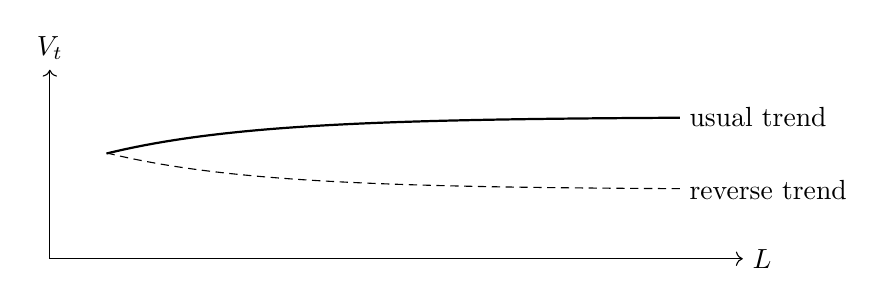
\begin{tikzpicture}[x=1.6cm,y=0.8cm]
 \draw[->] (0,0)--(5.5,0) node[right] {\(L\)};
 \draw[->] (0,0)--(0,3) node[above] {\(V_t\)};
 \draw[thick,domain=0.45:5,samples=60] plot (\x,{2.25-0.85*exp(-0.85*\x)});
 \draw[densely dashed,domain=0.45:5,samples=60] plot (\x,{1.1+0.85*exp(-0.85*\x)});
 \node[right] at (5,2.25) {usual trend};
 \node[right] at (5,1.1) {reverse trend};
\end{tikzpicture}
\end{latin}
\caption{طرح کیفی جهت تغییر آستانه با طول در دو رفتار توصیف‌شده در کتاب
و اسلاید ۲۰
\cite[بخش \secnum{۲.۴.۳.۳}]{weste}\cite{nonideal}.}
\label{fig:threshold-length-schematic}
\end{figure}

نام‌گذاری این قسمت از قرارداد کتاب برای وابستگی آستانه به طول پیروی
می‌کند. کتاب به کاربرد گسترده‌تر اصطلاح \lr{Short Channel Effect} برای
مجموعه اثرهای کانال کوتاه نیز اشاره می‌کند
\cite[پانوشت صفحه چاپی ۸۰]{weste}.

کتاب همچنین \lr{Narrow Channel Effect} را ذکر می‌کند که در آن آستانه
با عرض کانال تغییر می‌کند. اثر عرض معمولاً در مقایسه مورد بحث مرجع
کمتر است، زیرا حداقل عرض از حداقل طول بزرگ‌تر در نظر گرفته شده است
\cite[صفحه چاپی ۸۰]{weste}. مقدار و جهت وابستگی در یک افزاره مشخص به
ساختار و فرایند آن وابسته است.

با تغییر طول، ضریب \(\beta=\mu C_{\mathrm{ox}}W/L\) نیز تغییر می‌کند.
اگر مسئله، آستانه را تابع طول داده باشد، هم ضریب هندسی و هم
اضافه‌ولتاژ \(V_{GS}-V_t(L)\) باید به‌روزرسانی شوند.
در \lr{Channel Length Modulation} بخش \ref{sec:clm}، تغییر طول مؤثر
در اثر تغییر بایاس درین یک افزاره بررسی شد. در این قسمت، آستانه
افزاره‌ها با طول‌های مختلف مقایسه می‌شود.

در جدول \ref{tab:threshold-effects-summary} شرایط مقایسه سه اثر
گردآوری شده‌اند. علامت‌ها با قرارداد \lr{nMOS} بیان شده‌اند.
\begin{table}[!htbp]
\centering
\small
\caption{جهت تغییر آستانه در سه اثر این بخش، با ثابت بودن دیگر شرایط مقایسه.}
\label{tab:threshold-effects-summary}
\begin{tabularx}{\linewidth}{>{\raggedleft\arraybackslash}Xcc}
\toprule
اثر & متغیر مقایسه & نتیجه مدل\\
\midrule
\lr{Body Effect} & افزایش \(V_{SB}\) & افزایش \(V_t\)\\
\lr{DIBL} & افزایش \(V_{DS}\) & کاهش \(V_t\)\\
\lr{Short Channel Effect} معمول & کاهش \(L\) & کاهش \(V_t\)\\
رفتار \lr{Reverse Short Channel} & کاهش \(L\) & افزایش \(V_t\)\\
\bottomrule
\end{tabularx}
\end{table}

% !TeX root = booklet-02.tex
\subsection{جریان‌های نشتی}
\label{sec:leakage}
در افزاره واقعی، بایاس خاموش نیز با جریان‌های کوچکی همراه است. کتاب
سه مسیر اصلی را معرفی می‌کند. \lr{Subthreshold Leakage} در مسیر سورس
و درین، \lr{Gate Leakage} از راه عایق گیت و \lr{Junction Leakage} در
پیوندهای ناحیه‌های \lr{Diffusion} و بدنه جریان دارند
\cite[بخش \secnum{۲.۴.۴} و شکل \secnum{۲.۱۹}]{weste}
\cite[اسلایدهای ۲۱ و ۲۲]{nonideal}. بایاس، دما، هندسه و ساختار فرایند،
سهم هر مسیر را تعیین می‌کنند.

در روایت فناوری کتاب سال ۲۰۱۱، نشتی در نمونه‌های با ابعاد بالاتر از
\(\qty{180}{\nano\metre}\) معمولاً سهم کوچکی داشته است. برای نمونه‌های
\(\qty{90}{\nano\metre}\) و \(\qty{65}{\nano\metre}\)، جریان‌های
زیرآستانه در مرتبه یک تا چند ده نانوآمپر برای هر ترانزیستور گزارش
شده‌اند. در نمونه‌های \(\qty{45}{\nano\metre}\)، نازک‌شدن عایق، نشتی
گیت را نیز مهم می‌کند و مرجع نقش عایق‌های \lr{High-k} را مطرح می‌کند
\cite[صفحه ۸۱]{weste}. این اعداد به نمونه‌ها و زمان مرجع مربوط‌اند.

\subsubsection{\lr{Subthreshold Leakage}}
\label{sec:subthreshold-leakage}
\paragraph*{وارونگی ضعیف و معنای خاموشی}
در \lr{Weak Inversion}، ولتاژ گیت زیر آستانه است و مقدار جریان به‌صورت
نمایی با ولتاژ گیت تغییر می‌کند. در توصیف کتاب، عبور حرارتی حامل‌ها
از سد پتانسیل، جریان زیرآستانه را ایجاد می‌کند
\cite[بخش \secnum{۲.۴.۴.۱}]{weste}. در مدل سوئیچی، خروجی منطقی بر
اساس مسیرهای روشن و خاموش تحلیل می‌شود. مدل نشتی، مقدار جریان کوچک
مسیر خاموش و اثر آن بر توان و نگهداری بار را نیز محاسبه می‌کند.

\paragraph*{پیش‌نیاز تابع نمایی و لگاریتم ده‌دهی}
عدد \(e\approx2.71828\) پایه لگاریتم طبیعی است. تابع
\(\exp(x)=e^x\) برای هر \(x\) مثبت است. برای نمونه،
\(e^0=1\)، \(e^1\approx2.718\)، \(e^{-1}=1/e\approx0.368\) و
\(e^{-3}\approx0.0498\). منفی‌ترشدن توان، مقدار تابع را کوچک‌تر می‌کند.
قانون \(e^{a+b}=e^ae^b\) و در نتیجه \(e^a/e^b=e^{a-b}\) در محاسبه
نسبت نشتی‌ها به کار می‌روند.

لگاریتم ده‌دهی \(\log_{10}x\)، توانی از ده است که عدد \(x>0\) را
می‌سازد. مثلاً \(\log_{10}1000=3\) و \(\log_{10}0.01=-2\).
یک \lr{Decade} تغییر جریان یعنی ضرب یا تقسیم آن در ده.
برای تبدیل پایه از رابطه \(\log_{10}x=\ln x/\ln10\) استفاده می‌کنیم.
همچنین \(e^x=10^{x/\ln10}\) است. نسبت‌های داخل لگاریتم و توان تابع
نمایی باید بی‌بعد باشند.

\paragraph*{مدل جریان و تعریف همه پارامترها}
رابطه \secnum{۲.۴۲} کتاب و اسلاید ۲۳ برای \lr{nMOS} با
\(V_{DS}\ge0\) چنین بازنویسی می‌شود
\begin{equation}
 I_{\mathrm{sub}}=I_{ds0}
 \exp\!\left(\frac{V_{GS}-V_{t0}+\eta V_{DS}-k_\gamma V_{SB}}{nv_T}\right)
 \left(1-e^{-V_{DS}/v_T}\right).
 \label{eq:leakage-subthreshold-model}
\end{equation}
در این رابطه، \(V_{t0}\) آستانه مرجع، \(\eta\) ضریب \lr{DIBL} و
\(k_\gamma\) ضریب خطی اثر بدنه از
\eqref{eq:body-linearization} هستند. \(n>0\) ضریب وابسته به فرایند
است که مرجع مقدار معمول آن را حدود \num{1.3} تا \num{1.7} می‌گیرد.
\(v_T=kT/q\) ولتاژ حرارتی است. \(I_{ds0}\) ضریب جریان وابسته به
فرایند و هندسه است \cite[صفحات ۸۱ و ۸۲]{weste}.

صورت کسر داخل نمایی، یک ولتاژ است. مخرج \(nv_T\) نیز ولتاژ است، پس
توان بی‌بعد می‌شود. عامل آخر هم بی‌بعد است و واحد کل جریان از
\(I_{ds0}\) به دست می‌آید. برای استفاده از آستانه مؤثر، می‌توان
\(V_{t,\mathrm{eff}}=V_{t0}-\eta V_{DS}+k_\gamma V_{SB}\) را تعریف کرد
و صورت توان را \(V_{GS}-V_{t,\mathrm{eff}}\) نوشت.
این صورت از تقریب خطی بایاس بدنه استفاده می‌کند و دامنه آن با
\eqref{eq:body-linear-error} سنجیده می‌شود.

مدل مرجع، ضریب جریان را با رابطه تجربی زیر نیز تقریب می‌زند
\begin{equation}
 I_{ds0}=\beta v_T^2e^{1.8},\qquad
 \beta=\mu C_{\mathrm{ox}}\frac{W}{L}.
 \label{eq:leakage-current-prefactor}
\end{equation}
عدد \(1.8\) ضریب تجربی همان مدل است
\cite[رابطه \secnum{۲.۴۳}]{weste}. حاصل‌ضرب
\(\beta\) با واحد \(\unit{\ampere\per\volt\squared}\) و \(v_T^2\)،
واحد آمپر دارد. در شرایطی که صورت توان صفر و
\(V_{DS}\gg v_T\) باشد، جریان به \(I_{ds0}\) نزدیک می‌شود.
پارامترهای این رابطه می‌توانند با دما و فرایند تغییر کنند.

\paragraph*{عامل درین و معیار تقریب آن}
برای بررسی عامل آخر، \(D=V_{DS}\) و
\(F(D)=1-e^{-D/v_T}\) را تعریف می‌کنیم. در \(D=0\)، عامل \(F\)
صفر و جریان مدل نیز صفر است. با افزایش \(D>0\)، این عامل به یک
نزدیک می‌شود. چند مقدار در جدول \ref{tab:leakage-drain-factor}
آمده‌اند.
\begin{table}[!htbp]
\centering
\small
\caption{عامل درین در مدل زیرآستانه و فاصله نسبی آن از یک.}
\label{tab:leakage-drain-factor}
\begin{tabular}{cccc}
\toprule
\(D/v_T\) & \(e^{-D/v_T}\) & \(F(D)\) & فاصله از یک، درصد\\
\midrule
\num{1} & \num{0.3679} & \num{0.6321} & \num{36.79}\\
\num{2} & \num{0.1353} & \num{0.8647} & \num{13.53}\\
\num{3} & \num{0.0498} & \num{0.9502} & \num{4.98}\\
\num{5} & \num{0.00674} & \num{0.99326} & \num{0.674}\\
\bottomrule
\end{tabular}
\end{table}

برای فاصله حداکثر ۱ درصد از یک، باید
\(e^{-D/v_T}\le0.01\) باشد. با لگاریتم‌گیری،
\(D\ge-v_T\ln0.01\approx4.605v_T\) به دست می‌آید.
در \(v_T=\qty{26}{\milli\volt}\)، این شرط حدود
\(D\ge\qty{120}{\milli\volt}\) است. در
\(D=\qty{50}{\milli\volt}\)، عامل برابر \(0.8538\) و در
\(D=\qty{100}{\milli\volt}\)، برابر \(0.9786\) است.
در استفاده از تعبیر «چند برابر ولتاژ حرارتی» در متن مرجع، دقت مورد
نیاز محاسبه تعیین‌کننده انتخاب تقریب است.

در \(D\ll v_T\)، تقریب \(e^{-D/v_T}\approx1-D/v_T\) می‌دهد
\(F(D)\approx D/v_T\). ازاین‌رو، جریان در نزدیکی درین صفر با
\(D\) متناسب می‌شود. در \(D\gg v_T\)، عامل \(F\) تقریباً ثابت
است، اما جمله \(\eta D\) در توان هنوز می‌تواند با افزایش درین،
نشتی را افزایش دهد.

\paragraph*{مثال آموزشی مقدار جریان و اثر گیت}
فرض کنید \(\beta=\qty{1}{\milli\ampere\per\volt\squared}\)،
\(n=1.4\)، \(v_T=\qty{0.026}{\volt}\)،
\(V_{t0}=\qty{0.35}{\volt}\)، \(\eta=0.05\)،
\(V_{DS}=\qty{1}{\volt}\) و \(V_{SB}=0\) باشند.
این پارامترها برای یک مثال آموزشی فرض شده‌اند. ابتدا داریم
\begin{equation}
 I_{ds0}=(10^{-3})(0.026)^2e^{1.8}\,\unit{\ampere}
 \approx\qty{4.090}{\micro\ampere}.
 \label{eq:leakage-prefactor-example}
\end{equation}
در \(V_{GS}=0\)، صورت توان
\(-0.35+0.05(1)=-\qty{0.30}{\volt}\) و مخرج
\(1.4(0.026)=\qty{0.0364}{\volt}\) است.
چون \(F(\qty{1}{\volt})\approx1\)، جریان برابر است با
\begin{equation}
 I_{\mathrm{off}}\approx(4.090\times10^{-6})e^{-0.30/0.0364}
 \approx\qty{1.077}{\nano\ampere}.
 \label{eq:leakage-absolute-example}
\end{equation}
اگر فقط گیت به \(\qty{0.1}{\volt}\) برسد، نسبت دو جریان از قانون
تقسیم توابع نمایی به دست می‌آید
\begin{equation}
 \frac{I(\qty{0.1}{\volt})}{I(0)}
 =e^{0.1/0.0364}\approx15.60,
 \qquad I(\qty{0.1}{\volt})\approx\qty{16.81}{\nano\ampere}.
 \label{eq:leakage-gate-ratio-example}
\end{equation}
آستانه مؤثر در هر دو نقطه \(\qty{0.30}{\volt}\) است و هر دو بایاس
گیت در دامنه زیرآستانه قرار دارند.

\paragraph*{استخراج \lr{Subthreshold Slope} و خواندن نمودار لگاریتمی}
در بایاس درین، بدنه و دمای ثابت، تمام عامل‌های مستقل از گیت را در یک
ضریب ثابت جمع می‌کنیم. برای یک جریان مرجع ثابت \(I_r>0\)، از
\eqref{eq:leakage-subthreshold-model} نتیجه می‌شود
\begin{equation}
 y=\log_{10}\!\left(\frac{I_{\mathrm{sub}}}{I_r}\right)
 =c+\frac{V_{GS}}{nv_T\ln10}.
 \label{eq:leakage-log-line}
\end{equation}
نماد \(c\) یک مقدار ثابت در این مقایسه است. پس نمودار \(y\) برحسب
\(V_{GS}\) خطی است و شیب آن \(1/(nv_T\ln10)\) می‌شود.
کتاب معکوس این شیب را \lr{Subthreshold Slope} می‌نامد
\begin{equation}
 \boxed{S=\left[\frac{\mathrm{d}\log_{10}(I_{\mathrm{sub}}/I_r)}
 {\mathrm{d}V_{GS}}\right]^{-1}=nv_T\ln10}.
 \label{eq:leakage-subthreshold-slope}
\end{equation}
این رابطه با \secnum{۲.۴۴} کتاب و اسلاید ۲۳ متناظر است
\cite{weste,nonideal}. \(S\) تغییر گیت لازم برای ده‌برابرشدن جریان
است و معمولاً با واحد \(\unit{\milli\volt}\) به ازای یک
\lr{Decade} بیان می‌شود. در مثال قبل،
\(S=1.4(0.026)\ln10\approx\qty{83.81}{\milli\volt}\) است.
افزایش گیت به اندازه \(2S\)، جریان را صد برابر می‌کند.

شکل \ref{fig:leakage-semilog} نسبت جریان به مقدار گیت صفر را برای
همین \(S\) نشان می‌دهد. فاصله برابر روی محور عمودی لگاریتمی، به معنای
ضریب برابر در جریان است. برای \(n\) بین \num{1.3} و \num{1.7} و
\(v_T=\qty{26}{\milli\volt}\)، مقدار \(S\) حدود
\(\qty{77.8}{\milli\volt}\) تا \(\qty{101.8}{\milli\volt}\) به ازای هر دهه است.
\begin{figure}[!htbp]
\centering
\begin{latin}
\PersianMathDigits
\begin{tikzpicture}[x=22cm,y=1.05cm]
 \draw[->] (-0.12,-1.5)--(0.24,-1.5) node[right] {\(V_{GS}\;(\mathrm{V})\)};
 \draw[->] (-0.12,-1.5)--(-0.12,2.8) node[above] {\(I/I_{\mathrm{off}}\)};
 \foreach \x in {-0.1,0,0.1,0.2} {\draw (\x,-1.5)--(\x,-1.56) node[below] {\(\x\)};}
 \foreach \y/\value in {-1/0.1,0/1,1/10,2/100} {
  \draw (-0.12,\y)--(-0.125,\y) node[left] {\(\value\)};
 }
 \draw[thick,domain=-0.1:0.2,samples=50] plot (\x,{\x/0.0838141});
 \draw[dotted] (0,0)--(0.0838141,0)--(0.0838141,1)--(0,1);
 \draw[<->] (0,0.15)--(0.0838141,0.15) node[midway,above] {\(S\)};
\end{tikzpicture}
\end{latin}
\caption{نمودار آموزشی زیرآستانه با محور عمودی لگاریتمی و
\(S=\qty{83.81}{\milli\volt}\) به ازای هر دهه. گیت به اندازه \(S\)
تغییر می‌کند و نسبت جریان از یک به ده می‌رسد. بایاس‌های دیگر ثابت‌اند.}
\label{fig:leakage-semilog}
\end{figure}

در شکل \secnum{۲.۲۰} کتاب، محور عمودی جریان بر واحد عرض با واحد
\(\unit{\ampere\per\micro\metre}\) است. برای نمونه
\(\qty{65}{\nano\metre}\) در دمای \(\qty{70}{\degreeCelsius}\)،
مقادیر حدود \(\qty{27}{\nano\ampere\per\micro\metre}\) و
\(\qty{2}{\nano\ampere\per\micro\metre}\) در گیت صفر و دو بایاس
درین \(\qty{1.0}{\volt}\) و \(\qty{0.1}{\volt}\) مشخص شده‌اند.
نسبت آن‌ها حدود \(13.5\) است. بخش تقریباً خطی منحنی زیرآستانه و
بالارفتن جریان در گیت بسیار منفی، به‌ترتیب رفتار نمایی و اثر
\lr{GIDL} را نشان می‌دهند \cite[صفحه ۸۱]{weste}.

\paragraph*{بازنویسی دقیق نسبت به \(I_{\mathrm{off}}\)}
جریان مرجع را در گیت و بایاس بدنه صفر و درین \(V_{DD}>0\) تعریف
می‌کنیم. از \eqref{eq:leakage-subthreshold-model} داریم
\begin{equation}
 I_{\mathrm{off}}=I_{ds0}
 e^{(-V_{t0}+\eta V_{DD})/(nv_T)}F(V_{DD}).
 \label{eq:leakage-off-definition}
\end{equation}
تقسیم رابطه جریان بر رابطه مرجع، عامل \(I_{ds0}\) و آستانه مرجع را
حذف می‌کند. با استفاده از \(S=nv_T\ln10\)، نتیجه برابر است با
\begin{equation}
 \boxed{I_{\mathrm{sub}}=I_{\mathrm{off}}
 10^{[V_{GS}+\eta(V_{DS}-V_{DD})-k_\gamma V_{SB}]/S}
 \frac{F(V_{DS})}{F(V_{DD})}}.
 \label{eq:leakage-off-normalized}
\end{equation}
در بایاس مرجع، توان صفر و نسبت دو عامل \(F\) برابر یک است و جریان
مرجع دقیقاً بازیابی می‌شود. در بازنویسی رابطه \secnum{۲.۴۵} کتاب،
عامل مخرج با فرض \(V_{DD}\gg v_T\) تقریباً یک گرفته شده است.
برای نگه‌داشتن همه عامل‌ها در بایاس درین کوچک، از
\eqref{eq:leakage-off-normalized} استفاده می‌کنیم.

این نسبت برای هندسه، دما و پارامترهای یکسان نوشته شده است.
در یک دمای ثابت، افزایش \(V_{t0}\) به اندازه \(\Delta V_t>0\)،
جریان را در عامل \(e^{-\Delta V_t/(nv_T)}\) ضرب می‌کند.
افزایش بایاس بدنه در تقریب خطی، عامل
\(e^{-k_\gamma\Delta V_{SB}/(nv_T)}\) و تغییر درین، هم عامل نمایی
\lr{DIBL} و هم نسبت دو \(F\) را وارد می‌کند.
برای \lr{pMOS} با قرارداد بزرگی‌های مثبت، همین ساختار با
\(V_{SG},V_{SD},V_{BS}\)، بزرگی آستانه و پارامترهای آن افزاره به کار
می‌رود.

\paragraph*{حل مثال \secnum{۲.۶} کتاب و نسبت هزاربرابری}
مثال مرجع می‌خواهد جریان گیت صفر، هزار برابر کوچک‌تر از جریان در
گیت برابر آستانه باشد. در یک بایاس درین ثابت با \(V_{DS}\gg v_T\)،
بایاس بدنه صفر و با قرارداد آستانه همان مقایسه، نسبت جریان‌ها چنین است
\begin{equation}
 \frac{I(0)}{I(V_t)}=e^{-V_t/(nv_T)}=10^{-3}.
 \label{eq:leakage-three-decades}
\end{equation}
از دو طرف لگاریتم می‌گیریم. با \(\ln10^{-3}=-3\ln10\)، داریم
\begin{equation}
 -\frac{V_t}{nv_T}=-3\ln10
 \quad\Longrightarrow\quad V_t=3nv_T\ln10=3S.
 \label{eq:leakage-minimum-threshold}
\end{equation}
پس برای \(n=1.5\) و \(v_T=\qty{26}{\milli\volt}\)،
\(S\approx\qty{89.8}{\milli\volt}\) و
\(V_t\approx\qty{269.4}{\milli\volt}\) است. گردکردن مرجع حدود
\(\qty{270}{\milli\volt}\) می‌دهد. برای نمونه \lr{Silicon-on-Insulator
(SOI)} مثال با \(n=1.3\)، مقدار \(S\approx\qty{77.8}{\milli\volt}\)
و \(V_t\approx\qty{233.5}{\milli\volt}\) می‌شود
\cite[مثال \secnum{۲.۶}، صفحه ۸۲]{weste}.
شرط حداقل آستانه برای نسبت حداکثر \(10^{-3}\)، همان
\(V_t\ge3S\) است.

\paragraph*{اثر بر توان و نگهداری بار}
توان ایستای دریافت‌شده از یک منبع ثابت از
\(P_{\mathrm{static}}=V_{DD}I_{\mathrm{supply}}\) به دست می‌آید.
در یک مثال فرضی با \(10^8\) ترانزیستور، کسر خاموش \(0.8\)، نشتی
متوسط هر ترانزیستور خاموش \(\qty{1}{\nano\ampere}\) و تغذیه
\(\qty{1}{\volt}\)، اگر این جریان‌ها سهم جمع‌پذیر همان منبع باشند،
جریان کل \(\qty{0.08}{\ampere}\) و توان \(\qty{80}{\milli\watt}\)
می‌شود. برای مدار مشخص، اتصال مسیرها و جریان دریافتی از هر منبع با
\lr{KCL} محاسبه می‌شود.

نشتی همچنین بار گره خازنی را در طول زمان تغییر می‌دهد. با جریان
تقریباً ثابت \(I\)، تغییر ولتاژ \(\Delta V\) روی ظرفیت \(C\) در زمان
\(t\approx C\Delta V/I\) رخ می‌دهد. مثلاً
\(C=\qty{10}{\femto\farad}\)، \(I=\qty{1}{\nano\ampere}\) و
\(\Delta V=\qty{0.2}{\volt}\)، زمان حدود \(\qty{2}{\micro\second}\)
می‌دهند. این برآورد آموزشی، حساسیت گره‌های ذخیره بار و نیاز به
\lr{Refresh} در حافظه پویا را توضیح می‌دهد
\cite[صفحه ۸۲]{weste}.

\subsubsection{\lr{Gate Leakage}}
\label{sec:gate-leakage}
\paragraph*{تونل‌زنی و دو سازوکار مرجع}
در عایق بسیار نازک، احتمال عبور کوانتومی حامل از سد عایق، جریان
تونل‌زنی ایجاد می‌کند. برای بیان مقیاس، کتاب عایق‌های نازک‌تر از حدود
\(\qty{1.5}{\nano\metre}\) تا \(\qty{2.0}{\nano\metre}\) را در این
بحث مطرح می‌کند. کتاب دو سازوکار \lr{Fowler-Nordheim (FN)
Tunneling} و \lr{Direct Tunneling} را معرفی می‌کند.
اولی در ولتاژ زیاد و ضخامت متوسط اهمیت پیدا می‌کند و در برنامه‌ریزی
\lr{EEPROM} به کار می‌رود. دومی در عایق نازک و ولتاژ پایین‌تر اهمیت
دارد \cite[بخش \secnum{۲.۴.۴.۲}]{weste}.

برای \lr{Direct Tunneling}، رابطه \secnum{۲.۴۷} کتاب و اسلاید ۲۴ را
با نام‌گذاری ضرایب مستقل می‌نویسیم
\begin{equation}
 I_{\mathrm{gate}}=WA_g
 \left(\frac{V_{DD}}{t_{\mathrm{ox}}}\right)^2
 \exp\!\left(-B_g\frac{t_{\mathrm{ox}}}{V_{DD}}\right).
 \label{eq:gate-tunneling-model}
\end{equation}
\(A_g,B_g\) همان ثابت‌های فناوری \(A,B\) در مرجع هستند.
زیرنویس‌ها برای تشخیص آن‌ها از ضرایب مدل پیوند به کار رفته‌اند.
\(W\) عرض و \(t_{\mathrm{ox}}\) ضخامت فیزیکی عایق در مدل است.
این مدل تجربی در شرایط بایاس و پارامترهای مربوط به برازش استفاده
می‌شود \cite[صفحه ۸۳]{weste}\cite[اسلاید ۲۴]{nonideal}.

با دستگاه طول متر، بی‌بعدبودن توان ایجاب می‌کند
\([B_g]=\unit{\volt\per\metre}\). چون
\(W(V_{DD}/t_{\mathrm{ox}})^2\) واحد
\(\mathrm{V}^2/\mathrm{m}\) دارد،
\([A_g]=\mathrm{A\,m\,V^{-2}}\) است. اگر ضرایب با نانومتر برازش
شده‌اند، ضخامت و واحد ضرایب نیز با همان قرارداد وارد می‌شوند.

\paragraph*{حساسیت ضخامت و مثال نسبت جریان}
در ولتاژ، عرض و ضرایب ثابت، برای دو ضخامت مثبت \(t_1,t_2\)، تقسیم
دو رابطه \eqref{eq:gate-tunneling-model} می‌دهد
\begin{equation}
 \frac{I_2}{I_1}=\left(\frac{t_1}{t_2}\right)^2
 \exp\!\left[\frac{B_g(t_1-t_2)}{V_{DD}}\right].
 \label{eq:gate-thickness-ratio}
\end{equation}
کاهش ضخامت، هم عامل مربعی و هم عامل نمایی را افزایش می‌دهد.
در مثال فرضی \(t_1=\qty{1.1}{\nano\metre}\)،
\(t_2=\qty{1.0}{\nano\metre}\)، \(V_{DD}=\qty{1}{\volt}\) و
\(B_g=\qty{10}{\volt\per\nano\metre}\)، نسبت برابر
\((1.1/1.0)^2e^1\approx3.29\) است. مقدار \(B_g\) در این مثال
آموزشی فرض شده است. برای جریان مطلق، مقدار \(A_g\) نیز لازم است.
با ثابت بودن دیگر پارامترها، دوبرابرشدن عرض در همین مدل جریان را
دو برابر می‌کند.

در متن مرجع، برای داده‌های مورد بحث، افزایش جریان حداقل با ضریب
حدود \(2.7\) به ازای کاهش یک آنگستروم ضخامت گزارش شده است.
کتاب مقیاس ضخامت \(\qty{1.05}{\nano\metre}\)، معادل \num{10.5} آنگستروم، و چگالی جریان
\(\qty{100}{\ampere\per\centi\metre\squared}\) و ضخامت حدود
\(\qty{0.3}{\nano\metre}\) برای هر لایه اتمی \lr{SiO2} را در توضیح
نمونه‌های همان دوره مطرح می‌کند \cite[صفحه ۸۳]{weste}.
این اعداد همراه ماده و شرایط نمودار مرجع تفسیر می‌شوند.

\paragraph*{ولتاژ، چگالی جریان و عایق \lr{High-k}}
در ضخامت ثابت، نسبت جریان در دو ولتاژ مثبت چنین است
\begin{equation}
 \frac{I(V_2)}{I(V_1)}=
 \left(\frac{V_2}{V_1}\right)^2
 \exp\!\left[B_gt_{\mathrm{ox}}
 \left(\frac{1}{V_1}-\frac{1}{V_2}\right)\right].
 \label{eq:gate-voltage-ratio}
\end{equation}
برای \(V_2>V_1\)، هر دو عامل نسبت را افزایش می‌دهند.
در شکل \secnum{۲.۲۱} کتاب، محور عمودی چگالی جریان گیت
\(J_G=I_{\mathrm{gate}}/A_{\mathrm{gate}}\) با واحد
\(\unit{\ampere\per\centi\metre\squared}\) است.
برای چگالی یکنواخت، جریان از ضرب چگالی در مساحت به دست می‌آید.
مثلاً \(J_G=\qty{1}{\ampere\per\centi\metre\squared}\) و مساحت
فرضی \(\qty{0.005}{\micro\metre\squared}
=\qty{5e-11}{\centi\metre\squared}\)، جریان
\(\qty{50}{\pico\ampere}\) می‌دهند.
در شکل زیرآستانه \secnum{۲.۲۰}، نرمال‌سازی با عرض انجام شده است.
واحد محور هر شکل، نحوه تبدیل به جریان کل را تعیین می‌کند.

برای جریان روشن زیاد، ظرفیت اکسید بر واحد سطح بزرگ مطلوب است.
از \(C_{\mathrm{ox}}=\varepsilon/t\)، افزایش \lr{Permittivity} عایق
امکان استفاده از ضخامت فیزیکی بیشتر را در ظرفیت یکسان فراهم می‌کند.
ضخامت معادل اکسید از \(\mathrm{EOT}=t\varepsilon_{\mathrm{ox}}/
\varepsilon\) به دست می‌آید. تونل‌زنی به ضخامت فیزیکی و ویژگی سد
ماده وابسته است، پس ضرایب نشتی نیز باید با ماده عایق سازگار باشند.
در نمونه‌های \lr{SiO2} مورد بحث کتاب، نشتی گیت \lr{nMOS} می‌تواند
در مرتبه ده برابر \lr{pMOS} باشد، زیرا حامل‌ها سدهای انرژی متفاوتی
دارند. مرجع وابستگی این رفتار به نوع عایق را یادآور می‌شود
\cite[صفحه ۸۳]{weste}.

\subsubsection{\lr{Junction Leakage}}
\label{sec:junction-leakage}
\paragraph*{مدل دیود و علامت ولتاژ پیوند}
پیوند ناحیه‌های \lr{Diffusion} با بدنه یا \lr{Well} و پیوند
\lr{Well} با \lr{Substrate} مانند دیود عمل می‌کنند.
در بایاس معمول، بدنه و \lr{Well} به زمین یا تغذیه متصل می‌شوند تا
پیوندها در بایاس صفر یا معکوس قرار گیرند
\cite[بخش \secnum{۲.۴.۴.۳} و شکل \secnum{۲.۲۲}]{weste}.
مدل دیود کتاب را با نماد \(I_{\mathrm{dio}}\) برای جریان و
\(I_{\mathrm{rev}}>0\) برای ضریب جریان معکوس بازنویسی می‌کنیم
\begin{equation}
 I_{\mathrm{dio}}=I_{\mathrm{rev}}
 \left(e^{V_{\mathrm{dio}}/v_T}-1\right),\qquad
 V_{\mathrm{dio}}=V_{\mathrm{anode}}-V_{\mathrm{cathode}}.
 \label{eq:junction-diode-model}
\end{equation}
این دو جریان با \(I_D,I_S\) رابطه \secnum{۲.۴۸} کتاب متناظرند.
نمادهای مرجع در این رابطه به جریان دیود و ضریب جریان معکوس اشاره
دارند \cite[صفحه ۸۴ و پانوشت آن]{weste}\cite[اسلاید ۲۶]{nonideal}.

در پیوند \lr{nMOS}، بدنه \lr{p-type} آند و ناحیه
\lr{n-type Diffusion} کاتد است. بنابراین برای پیوند درین و بدنه،
\(V_{\mathrm{dio}}=V_B-V_D=-V_{DB}\) است.
اگر \(V_{DB}>0\)، ولتاژ دیود منفی و جریان آن در قرارداد آند به
کاتد منفی می‌شود. در بایاس معکوس بزرگ‌تر از چند برابر \(v_T\)،
جمله نمایی به صفر نزدیک و
\(I_{\mathrm{dio}}\approx-I_{\mathrm{rev}}\) است.
جریان معکوس در این قرارداد از ناحیه درین به بدنه می‌رود.
در بایاس صفر نیز \(I_{\mathrm{dio}}=0\) حاصل می‌شود.

ضریب \(I_{\mathrm{rev}}\) به ناخالصی، مساحت و محیط ناحیه
\lr{Diffusion} وابسته است. کتاب برای مؤلفه معمول دیود، مرتبه
\(\qty{0.01}{\femto\ampere\per\micro\metre\squared}\) تا
\(\qty{0.1}{\femto\ampere\per\micro\metre\squared}\) را در
نمونه‌های مورد بحث ذکر می‌کند \cite[صفحه ۸۴]{weste}.
در مثال فرضی با چگالی \(\qty{0.1}{\femto\ampere\per\micro\metre\squared}\)،
مساحت \(\qty{0.2}{\micro\metre\squared}\) و صرف‌نظر از سهم محیط،
\(I_{\mathrm{rev}}=\qty{0.02}{\femto\ampere}\) می‌شود.
در بایاس معکوس \(\qty{1}{\volt}\) و
\(v_T=\qty{0.026}{\volt}\)، جریان حدود
\(-\qty{0.02}{\femto\ampere}\) است.

\paragraph*{\lr{Band-to-Band Tunneling} و نقش ناخالصی}
در پیوندهای با ناخالصی زیاد، میدان قوی می‌تواند
\lr{Band-to-Band Tunneling (BTBT)} ایجاد کند.
مرجع اثر \lr{Halo Doping}، یعنی افزایش ناخالصی نزدیک انتهای کانال
برای کنترل آستانه، را بر افزایش این نشتی توضیح می‌دهد.
وجود تله‌های ناشی از نقص ماده نیز می‌تواند
\lr{Trap-Assisted Tunneling (TAT)} را تقویت کند.
در توصیف کتاب، سهم مهمی از این جریان نزدیک دیواره پیوند رو به
کانال رخ می‌دهد \cite[صفحه ۸۴]{weste}\cite[اسلاید ۲۷]{nonideal}.

رابطه تجربی \secnum{۲.۴۹} کتاب برای بزرگی جریان چنین است
\begin{equation}
 I_{\mathrm{BTBT}}=WX_j A_b\frac{E_j}{E_g^{1/2}}V_{DD}
 \exp\!\left(-B_b\frac{E_g^{3/2}}{E_j}\right).
 \label{eq:junction-btbt-model}
\end{equation}
\(X_j\) عمق پیوند، \(E_j\) بزرگی میدان پیوند و \(A_b,B_b\)
ثابت‌های فناوری هستند. کتاب \(E_g\) را ولتاژ متناظر با گاف انرژی
تعریف می‌کند. اگر انرژی گاف برحسب ژول معلوم باشد، تقسیم آن بر
\(q\) مقدار \(E_g\) را برحسب ولت می‌دهد.
توان‌های \(1/2\) و \(3/2\) روی همین کمیت اعمال می‌شوند.
در قرارداد طول متر، بی‌بعدبودن توان و واحد آمپر نتیجه می‌دهند
\begin{equation}
 [B_b]=\mathrm{m}^{-1}\mathrm{V}^{-1/2},\qquad
 [A_b]=\mathrm{A\,m}^{-1}\mathrm{V}^{-3/2}.
 \label{eq:junction-btbt-units}
\end{equation}
ضرایب \(A_b,B_b\) با \(A_g,B_g\) مدل گیت جداگانه تعریف و برازش
می‌شوند.

\paragraph*{میدان پیوند و یک محاسبه آموزشی}
در بایاس معکوس \(V_{DD}\)، رابطه \secnum{۲.۵۰} کتاب میدان را با
ناخالصی \lr{Halo} و \lr{Source/Drain} مرتبط می‌کند
\begin{equation}
 E_j=\sqrt{\frac{2qN_{\mathrm{halo}}N_{\mathrm{sd}}}
 {\varepsilon_{\mathrm{si}}(N_{\mathrm{halo}}+N_{\mathrm{sd}})}
 \left[V_{DD}+v_T\ln\!\left(
 \frac{N_{\mathrm{halo}}N_{\mathrm{sd}}}{n_i^2}\right)\right]}.
 \label{eq:junction-field-model}
\end{equation}
همه غلظت‌ها باید با واحد یکسان و \(\varepsilon_{\mathrm{si}}\) با
واحد طول سازگار وارد شوند. برای دنبال‌کردن محاسبه،
دو کمیت کمکی را تعریف می‌کنیم
\begin{equation}
 N_{\mathrm{eff}}=\frac{N_{\mathrm{halo}}N_{\mathrm{sd}}}
 {N_{\mathrm{halo}}+N_{\mathrm{sd}}},\qquad
 \phi_{\mathrm{bi}}=v_T\ln\!\left(
 \frac{N_{\mathrm{halo}}N_{\mathrm{sd}}}{n_i^2}\right).
 \label{eq:junction-field-parameters}
\end{equation}
با جایگذاری آن‌ها، رابطه میدان به شکل ساده‌تر زیر تبدیل می‌شود
\[
 E_j=\sqrt{\frac{2qN_{\mathrm{eff}}}{\varepsilon_{\mathrm{si}}}
 (V_{DD}+\phi_{\mathrm{bi}})}.
\]
\(\phi_{\mathrm{bi}}\) واحد ولت دارد و عبارت زیر رادیکال، واحد
\(\mathrm{V}^2/\mathrm{m}^2\) یا شکل سازگار سانتی‌متری آن را دارد.

در مثال فرضی، \(N_{\mathrm{halo}}=\qty{e18}{\per\centi\metre\cubed}\)،
\(N_{\mathrm{sd}}=\qty{e20}{\per\centi\metre\cubed}\)،
\(n_i=\qty{1.45e10}{\per\centi\metre\cubed}\)،
\(v_T=\qty{0.026}{\volt}\) و
\(\varepsilon_{\mathrm{si}}=11.7(\qty{8.85e-14}{\farad\per\centi\metre})\)
هستند. محاسبه می‌دهد
\begin{align}
 N_{\mathrm{eff}}&\approx\qty{9.901e17}{\per\centi\metre\cubed},
 &\phi_{\mathrm{bi}}&\approx\qty{1.0583}{\volt},\notag\\
 E_j(V_{DD}=\qty{0.8}{\volt})&\approx\qty{7.541e5}{\volt\per\centi\metre},
 &E_j(V_{DD}=\qty{1.2}{\volt})&\approx\qty{8.313e5}{\volt\per\centi\metre}.
 \label{eq:junction-field-example}
\end{align}
برای مشاهده حساسیت نمایی، حاصل‌ضرب فرضی
\(B_bE_g^{3/2}=\qty{3e6}{\volt\per\centi\metre}\) را ثابت می‌گیریم.
تقسیم دو جریان \eqref{eq:junction-btbt-model} با هندسه و گاف یکسان
می‌دهد
\begin{equation}
 \frac{I_2}{I_1}=
 \frac{1.2}{0.8}\frac{E_{j2}}{E_{j1}}
 \exp\!\left[3\times10^6
 \left(\frac{1}{E_{j1}}-\frac{1}{E_{j2}}\right)\right]
 \approx2.39.
 \label{eq:junction-btbt-ratio-example}
\end{equation}
در این جایگذاری عددی، میدان‌ها برحسب
\(\unit{\volt\per\centi\metre}\) وارد شده‌اند.
برای جریان مطلق، ثابت \(A_b\) و دیگر پارامترهای همان فناوری لازم‌اند.

\paragraph*{\lr{Gate-Induced Drain Leakage}}
\lr{Gate-Induced Drain Leakage (GIDL)} نزدیک ناحیه هم‌پوشانی گیت و
درین رخ می‌دهد. درین بالا و گیت پایین، میدان این ناحیه را تقویت
می‌کنند. در \lr{nMOS}، منفی‌ترکردن گیت در درین بالا می‌تواند این
مسیر را شدیدتر کند. جریان به ناحیه هم‌پوشانی و در نتیجه به عرض
افزاره وابسته است \cite[صفحات ۸۴ و ابتدای ۸۵]{weste}
\cite[اسلاید ۲۸]{nonideal}.
در توصیف نمونه‌های کتاب، سهم این مسیر در
\(|V_{GD}|\le V_{DD}\) معمولاً کوچک است و با راندن گیت بیرون ریل
تغذیه برجسته می‌شود.

برای مثال، در \(V_D=\qty{1}{\volt}\)، تغییر گیت از صفر به
\(-\qty{0.3}{\volt}\)، ولتاژ \(V_{DG}=V_D-V_G\) را از
\(\qty{1}{\volt}\) به \(\qty{1.3}{\volt}\) می‌رساند.
در مدل زیرآستانه، گیت منفی جریان سورس و درین را کاهش می‌دهد، اما
میدان درین و گیت در همین تغییر افزایش می‌یابد.
شکل \secnum{۲.۲۰} کتاب بالا رفتن جریان در سمت گیت منفی را نشان
می‌دهد. برای محاسبه کل نشتی در آن بایاس، همه مسیرهای مربوط به
بایاس و جریان دریافتی از منبع باید در مدل مدار لحاظ شوند.

% !TeX root = booklet-02.tex
\clearpage
\subsection{وابستگی به دما}
\label{sec:temperature-dependence}
افزایش دما، هم حرکت حامل‌ها و هم ولتاژ آستانه را تغییر می‌دهد. برای
محاسبه جریان، باید این تغییرها را هم‌زمان وارد مدل کرد
\cite[بخش \secnum{۲.۴.۵}، صفحات ۸۵ و ۸۶]{weste}
\cite[اسلاید ۲۹]{nonideal}. در این بخش، \(T\) دمای مطلق، \(T_r\)
دمای مرجع و \(\mu\) همان \lr{Mobility} مورد استفاده در مدل جریان است.

\subsubsection*{دمای مطلق، توان منفی و کاهش \lr{Mobility}}
ارتباط دمای سلسیوس \(t_C\) با دمای مطلق به صورت زیر است.
\[
 T/\unit{\kelvin}=t_C/\unit{\degreeCelsius}+273.15.
\]
مثلاً \(\qty{300}{\kelvin}\) برابر \(\qty{26.85}{\degreeCelsius}\)
است. اختلاف دمای یک کلوین با اختلاف یک درجه سلسیوس برابر است.
در نسبت دماها باید مقدار کلوین را به کار برد. نسبت دماهای سلسیوس
معنای مورد نیاز رابطه \eqref{eq:temperature-mobility} را ندارد.

تقریب تجربی رابطه \secnum{۲.۵۱} کتاب چنین است
\begin{equation}
 \boxed{\mu(T)=\mu(T_r)\left(\frac{T}{T_r}\right)^{-k_\mu}}.
 \label{eq:temperature-mobility}
\end{equation}
ضریب \(k_\mu\) بی‌بعد است و مرجع مقدار معمول آن را حدود \(1.5\)
می‌گیرد. هر دو طرف رابطه واحد \lr{Mobility} دارند. توان منفی یعنی
\(x^{-a}=1/x^a\). بنابراین، برای \(T>T_r\) و \(k_\mu>0\)، نسبت
\(\mu(T)/\mu(T_r)\) از یک کوچک‌تر می‌شود. تفسیر فیزیکی آن کاهش
حرکت‌پذیری حامل‌ها در اثر افزایش پراکندگی با گرم‌شدن شبکه است.

برای نمونه، با \(T_r=\qty{300}{\kelvin}\)،
\(T=\qty{400}{\kelvin}\) و \(k_\mu=1.5\)، داریم
\begin{equation}
 \frac{\mu(400)}{\mu(300)}
 =\left(\frac{4}{3}\right)^{-3/2}
 =\frac{1}{(4/3)\sqrt{4/3}}\approx0.6495.
 \label{eq:temperature-mobility-example}
\end{equation}
در این تقریب، \lr{Mobility} حدود \num{35.05} درصد کاهش یافته است.
عددهای داخل آرگومان \(\mu\) در این مثال برحسب کلوین‌اند.
با ثابت‌گرفتن \(C_{\mathrm{ox}}\) و هندسه، ضریب
\(\beta(T)=\mu(T)C_{\mathrm{ox}}W/L\) نیز همین نسبت را دارد.

\subsubsection*{آستانه و سرعت اشباع}
تقریب رابطه \secnum{۲.۵۲} کتاب برای آستانه \lr{nMOS} برابر است با
\begin{equation}
 \boxed{V_t(T)=V_t(T_r)-k_{vt}(T-T_r)}.
 \label{eq:temperature-threshold}
\end{equation}
ضریب مثبت \(k_{vt}\) واحد \(\unit{\volt\per\kelvin}\) دارد و مقدار
معمول آن در مرجع حدود \(\qty{1}{\milli\volt\per\kelvin}\) تا
\(\qty{2}{\milli\volt\per\kelvin}\) است. حاصل‌ضرب آن در اختلاف
دما یک ولتاژ است. برای \lr{pMOS}، همین نوع تقریب را بر بزرگی آستانه
\(V_{TP}=|V_{tp}|\) اعمال می‌کنیم. کاهش بزرگی آستانه منفی، مقدار
علامت‌دار \(V_{tp}\) را به صفر نزدیک می‌کند.

اگر \(V_t(300)=\qty{0.4}{\volt}\) و
\(k_{vt}=\qty{1}{\milli\volt\per\kelvin}\) فرض شوند، افزایش دما
به اندازه \(\qty{100}{\kelvin}\)، آستانه را
\(\qty{0.1}{\volt}\) کاهش می‌دهد و
\(V_t(400)=\qty{0.3}{\volt}\) می‌شود. در گیت ثابت، این تغییر،
اضافه‌ولتاژ \(V_{GS}-V_t\) را افزایش می‌دهد و جریان روشن را تقویت
می‌کند. در همان زمان، کاهش \lr{Mobility} جریان را تضعیف می‌کند.

سرعت اشباع \(v_{\mathrm{sat}}\) هم با افزایش دما کاهش می‌یابد.
کتاب برای افزایش دما از \(\qty{300}{\kelvin}\) به
\(\qty{400}{\kelvin}\)، کاهش حدود ۲۰ درصد را بیان می‌کند
\cite[صفحه ۸۵]{weste}. این اعداد پارامترهای تقریبی وابسته به فناوری‌اند.
در مدل میدان قوی، تغییر \(\mu\) باید در \(\beta\) و تغییر
\(v_{\mathrm{sat}}/\mu\) باید در \(E_c\) و \(V_c\) اعمال شود.

\subsubsection*{مثال آموزشی رقابت دو اثر در جریان روشن}
برای جداکردن نقش آستانه و \lr{Mobility}، از مدل مربعی اشباع استفاده
می‌کنیم. فرض‌های آموزشی عبارت‌اند از هندسه و
\(C_{\mathrm{ox}}\) ثابت، \(V_{SB}=0\)، صرف‌نظر از \lr{CLM} و
\lr{DIBL} و محدودیت سرعت، و مقادیر
\(T_r=\qty{300}{\kelvin}\)، \(k_\mu=1.5\)،
\(V_t(T_r)=\qty{0.4}{\volt}\)،
\(k_{vt}=\qty{0.001}{\volt\per\kelvin}\) و
\(\beta_r=\qty{200}{\micro\ampere\per\volt\squared}\).
در بایاس روشن \(V_{GS}=V_{DS}=V_{DD}\)، جای‌گذاری روابط دما می‌دهد
\begin{equation}
 I_{\mathrm{on}}(T)=\frac{\beta_r}{2}
 \left(\frac{T}{T_r}\right)^{-k_\mu}
 [V_{DD}-V_t(T_r)+k_{vt}(T-T_r)]^2.
 \label{eq:temperature-on-current}
\end{equation}
این رابطه برای \(V_{DD}>V_t(T)\) و ناحیه اشباع مدل به کار می‌رود.
چون در این مثال \(V_t(T)>0\) است، شرط
\(V_{DS}=V_{DD}\ge V_{DD}-V_t(T)\) برقرار می‌ماند.

با تعریف \(A_r=V_{DD}-V_t(T_r)\)، تقسیم جریان‌ها مراحل محاسبه را
آشکار می‌کند
\begin{equation}
 \frac{I_{\mathrm{on}}(T)}{I_{\mathrm{on}}(T_r)}
 =\left(\frac{T}{T_r}\right)^{-k_\mu}
 \left[1+\frac{k_{vt}(T-T_r)}{A_r}\right]^2.
 \label{eq:temperature-current-ratio}
\end{equation}
عامل نخست در دمای بالاتر کمتر از یک است. عامل دوم بزرگ‌تر از یک
می‌شود و برای \(A_r\) کوچک، اثر نسبی قوی‌تری دارد.
جدول \ref{tab:temperature-on-results} دو حالت را نشان می‌دهد.
\begin{table}[!htbp]
\centering
\small
\caption{جریان روشن در مثال آموزشی دما با مدل مربعی.}
\label{tab:temperature-on-results}
\begin{tabular}{ccccc}
\toprule
\(V_{DD}\)، \(\unit{\volt}\) & \(A_r\)، \(\unit{\volt}\) &
\(I(300)\)، \(\unit{\micro\ampere}\) &
\(I(400)\)، \(\unit{\micro\ampere}\) & \(I(400)/I(300)\)\\
\midrule
\num{1.2} & \num{0.8} & \num{64.00} & \num{52.61} & \num{0.8220}\\
\num{0.6} & \num{0.2} & \num{4.000} & \num{5.846} & \num{1.461}\\
\bottomrule
\end{tabular}
\end{table}
برای ردیف نخست، محاسبه نسبت برابر
\(0.6495(0.9/0.8)^2\) و برای ردیف دوم برابر
\(0.6495(0.3/0.2)^2\) است. در تغذیه بالاتر، کاهش
\lr{Mobility} غالب شده است. در تغذیه پایین‌تر، افزایش نسبی
اضافه‌ولتاژ گیت، جریان را افزایش داده است. شکل
\ref{fig:temperature-on-ratio} همین مدل را در بازه دما رسم می‌کند.
\begin{figure}[!htbp]
\centering
\begin{latin}
\PersianMathDigits
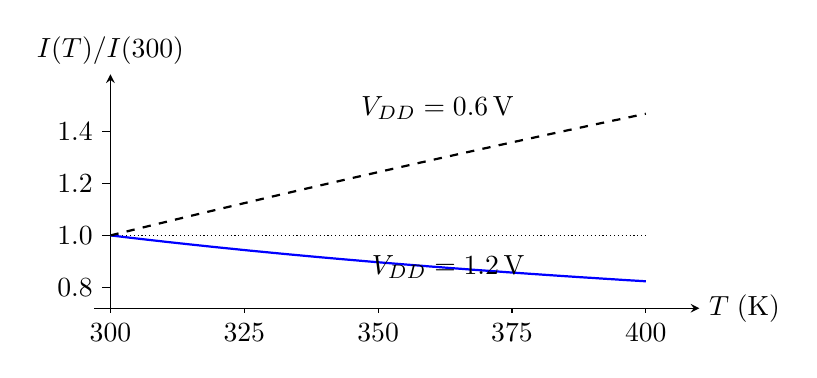
\begin{tikzpicture}[x=0.068cm,y=3.3cm,>=stealth]
\draw[->] (-3,0.72)--(110,0.72) node[right] {\(T\;(\mathrm{K})\)};
\draw[->] (0,0.72)--(0,1.62) node[above] {\(I(T)/I(300)\)};
\foreach \x/\t in {0/300,25/325,50/350,75/375,100/400}
 {\draw (\x,0.72)--(\x,0.70) node[below] {\(\t\)};}
\foreach \y in {0.8,1.0,1.2,1.4}
 {\draw (0,\y)--(-1.5,\y) node[left] {\(\y\)};}
\draw[densely dotted] (0,1)--(100,1);
\draw[thick,blue,domain=0:100,samples=70]
 plot (\x,{pow((300+\x)/300,-1.5)*pow((0.8+0.001*\x)/0.8,2)});
\draw[thick,dashed,domain=0:100,samples=70]
 plot (\x,{pow((300+\x)/300,-1.5)*pow((0.2+0.001*\x)/0.2,2)});
\node[anchor=west] at (47,0.88) {\(V_{DD}=1.2\,\mathrm{V}\)};
\node[anchor=west] at (45,1.49) {\(V_{DD}=0.6\,\mathrm{V}\)};
\end{tikzpicture}
\end{latin}
\caption{تغییر جریان نرمال‌شده برای پارامترهای فرضی مثال دما.
منحنی‌ها از رابطه \eqref{eq:temperature-current-ratio} محاسبه شده‌اند.}
\label{fig:temperature-on-ratio}
\end{figure}

\subsubsection*{معنای ضریب دمایی و استخراج شرط تغییر علامت}
مشتق \(\mathrm{d}I/\mathrm{d}T\)، نرخ تغییر جریان با تغییر کوچک
دماست. برای درک سهم عامل‌ها، می‌توان ابتدا تغییر نسبی را نوشت.
در مدل \eqref{eq:temperature-on-current}، جریان با \(\beta A^2\)
متناسب است که \(A(T)=V_{DD}-V_t(T)>0\) است. برای تغییر کوچک دما،
تغییر نسبی حاصل‌ضرب تقریباً برابر جمع تغییرهای نسبی عامل‌ها می‌شود
\begin{equation}
 \frac{\Delta I}{I}\approx
 \frac{\Delta\beta}{\beta}+2\frac{\Delta A}{A}.
 \label{eq:temperature-fractional-change}
\end{equation}
ضریب دو از مربع \(A\) می‌آید. مشتق دقیق همین بیان، با
\(\beta\propto T^{-k_\mu}\) و
\(\mathrm{d}A/\mathrm{d}T=k_{vt}\)، برابر است با
\begin{equation}
 \frac{1}{I}\frac{\mathrm{d}I}{\mathrm{d}T}
 =-\frac{k_\mu}{T}+\frac{2k_{vt}}{V_{DD}-V_t(T)}.
 \label{eq:temperature-coefficient}
\end{equation}
هر دو جمله واحد \(\unit{\per\kelvin}\) دارند. ضریب مثبت یعنی افزایش
جریان با گرم‌شدن در همسایگی همان نقطه. با صفرقراردادن طرف راست،
شرط توازن محلی به دست می‌آید
\begin{equation}
 V_{DD}-V_t(T)=\frac{2k_{vt}T}{k_\mu}.
 \label{eq:temperature-crossover}
\end{equation}
در \(\qty{300}{\kelvin}\) و با پارامترهای مثال، طرف راست
\(\qty{0.4}{\volt}\) است و توازن محلی در
\(V_{DD}=\qty{0.8}{\volt}\) رخ می‌دهد. این شرط، شیب جریان در یک
دمای مشخص را صفر می‌کند. برابری جریان در دو دمای با فاصله زیاد
باید مستقیماً از \eqref{eq:temperature-current-ratio} حل شود.

کتاب، رفتار معمول جریان روشن را در تغذیه بالا کاهشی توصیف می‌کند و
برای تغذیه پایین، افزایش جریان با دما را نیز مطرح می‌کند. بازه
تقریبی \(\qty{0.7}{\volt}\) تا \(\qty{1.1}{\volt}\) در متن کتاب به
نمونه‌های فناوری آن مرجع مربوط است. شکل‌های \secnum{۲.۲۳} و
\secnum{۲.۲۴} همان صفحه، تغییر شکل منحنی و کاهش معمول جریان روشن
را نمایش می‌دهند \cite[صفحه ۸۵]{weste}. تعیین نقطه تغییر علامت در
یک فناوری مشخص به مدل کامل همان فناوری نیاز دارد.

\subsubsection*{مثال آموزشی تغییر نشتی مطلق با دما}
در تمرین \secnum{۲.۱۰}، دو آستانه متفاوت در یک دمای مشترک مقایسه می‌شوند.
برای مقایسه دو دما، عامل پیش‌ضرب و ولتاژ حرارتی هم تغییر می‌کنند.
فرض کنید مدل \eqref{eq:leakage-subthreshold-model} با
\(V_{GS}=V_{SB}=0\)، \(V_{DS}=\qty{1}{\volt}\)، \(\eta=0\)،
\(n=1.4\) و همان \(\beta(T)\) و \(V_t(T)\) مثال دما به کار رود.
در این مدل آموزشی، \(n\)، هندسه و \(C_{\mathrm{ox}}\) ثابت‌اند.
اگر \(v_{T,i}=kT_i/q\) و
\(F_i=1-\exp(-V_{DS}/v_{T,i})\) باشند، تقسیم دو جریان می‌دهد
\begin{equation}
 \frac{I_2}{I_1}=
 \left(\frac{T_2}{T_1}\right)^{2-k_\mu}
 \exp\!\left[\frac{V_t(T_1)}{nv_{T,1}}
             -\frac{V_t(T_2)}{nv_{T,2}}\right]\frac{F_2}{F_1}.
 \label{eq:temperature-leakage-ratio}
\end{equation}
توان \(2-k_\mu\) از حاصل‌ضرب
\(\beta\propto T^{-k_\mu}\) و \(v_T^2\propto T^2\) در
\eqref{eq:leakage-current-prefactor} به دست آمده است.
ثابت تجربی \(e^{1.8}\) در نسبت حذف می‌شود.
با \(k/q\approx\qty{8.61733e-5}{\volt\per\kelvin}\)،
\(v_{T,1}\approx\qty{25.852}{\milli\volt}\) و
\(v_{T,2}\approx\qty{34.469}{\milli\volt}\) هستند.
در هر دو دما، \(V_{DS}/v_T>29\) و عامل \(F\) با دقت خوبی یک است.
جای‌گذاری \(V_t(300)=\qty{0.4}{\volt}\) و
\(V_t(400)=\qty{0.3}{\volt}\) نتیجه می‌دهد
\begin{equation}
 I_1\approx\qty{12.82}{\pico\ampere},\qquad
 I_2\approx\qty{1.864}{\nano\ampere},\qquad
 \frac{I_2}{I_1}\approx145.3.
 \label{eq:temperature-leakage-example}
\end{equation}
هر دو بایاس گیت زیر آستانه‌اند. رشد شدید در این مثال از تغییر عامل
نمایی ناشی می‌شود. مقدار واقعی رشد به پارامترها و بایاس وابسته است.
کتاب رشد شدید نشتی زیرآستانه، رشد آهسته‌تر \lr{BTBT} و وابستگی کم
نشتی گیت به دما را در محدوده بحث خود بیان می‌کند
\cite[صفحه ۸۵]{weste}. توان نشتی هر منبع از جریان همان منبع و
ولتاژ آن به دست می‌آید.

\subsubsection*{خنک‌کاری و سازگاری مدل میدان بحرانی}
کاهش دما معمولاً \lr{Mobility} را بیشتر و نشتی زیرآستانه را کمتر
می‌کند. مرجع، دفع گرما با همرفت، فن و \lr{Heat Sink} و روش‌های
قوی‌تر مانند خنک‌کاری آبی، سردکننده لایه‌نازک و نیتروژن مایع را
مطرح می‌کند. کاهش نشتی می‌تواند به انتخاب آستانه کمتر کمک کند.
متن همچنین افزایش پهنای ناحیه تخلیه و کاهش ظرفیت پیوند را در بحث
عملکرد دمای پایین بیان می‌کند \cite[صفحه ۸۶]{weste}.
این نتایج با فرض‌های بایاس و فناوری همان بحث تفسیر می‌شوند.

برای جهت تغییر \(E_c\)، رابطه \eqref{eq:critical-field} باید با هر
دو پارامتر بررسی شود. با تقریب‌های عددی همین بخش، داریم
\begin{equation}
 \frac{E_c(400)}{E_c(300)}
 =\frac{v_{\mathrm{sat}}(400)/v_{\mathrm{sat}}(300)}
        {\mu(400)/\mu(300)}
 \approx\frac{0.8}{0.6495}\approx1.232.
 \label{eq:temperature-critical-field}
\end{equation}
پس ترکیب این تقریب‌ها، میدان بحرانی بزرگ‌تر را در دمای بالاتر
می‌دهد. عبارت کیفی صفحه ۸۶ درباره وقوع اشباع سرعت در میدان‌های
بالاتر هنگام خنک‌کاری، با این انتخاب هم‌زمان پارامترها سازگار
نیست. در محاسبه این جزوه، جهت تغییر از نسبت
\(2v_{\mathrm{sat}}/\mu\) و داده‌های مدل تعیین می‌شود.

مرجع استفاده کوتاه‌مدت از اسپری سردکننده و دمنده هوای گرم را برای
تشخیص حساسیت دمایی مدار نیز بیان می‌کند و امکان آسیب ناشی از تغییر
ناگهانی دما به تراشه یا بسته‌بندی را یادآور می‌شود
\cite[صفحه ۸۶]{weste}. این توصیف، بخشی از محتوای مرجع است.

\clearpage
\subsection{وابستگی به هندسه}
\label{sec:geometry-dependence}
ابعاد ترسیم‌شده در \lr{Layout} با ابعاد مؤثر کانال تفاوت دارند.
کتاب و اسلایدها این تفاوت را با دو نوع اصلاح مدل می‌کنند
\cite[بخش \secnum{۲.۴.۶}، صفحه ۸۶]{weste}
\cite[اسلایدهای ۳۵ و ۳۶]{nonideal}. نمادهای
\(L_{\mathrm{drawn}},W_{\mathrm{drawn}}\) طول و عرض ترسیم‌شده‌اند.
اصلاح‌های علامت‌دار \(X_L,X_W\) تغییر ناشی از ساخت ماسک و فرایند
ساخت را نمایش می‌دهند. مثلاً \lr{Overetch} می‌تواند طول گیت را
کوتاه کند و \(X_L<0\) بدهد. پارامتر \(L_D\) سهم نفوذ جانبی از هر
طرف و \(W_D\) اصلاح کاهش عرض از هر لبه است.

\subsubsection*{استخراج ابعاد مؤثر و معنای ضریب دو}
پس از اصلاح ساخت، طول هندسی گیت
\(L_g=L_{\mathrm{drawn}}+X_L\) است. ناحیه‌های سورس و درین هر کدام
به اندازه \(L_D\) زیر گیت پیشروی می‌کنند. فاصله مؤثر عبور حامل‌ها
با کم‌کردن هر دو سهم به دست می‌آید. رابطه عرض نیز دو لبه دارد.
در نتیجه، رابطه \secnum{۲.۵۳} کتاب چنین نوشته می‌شود
\begin{align}
 L_{\mathrm{eff}}&=L_{\mathrm{drawn}}+X_L-2L_D,
 \label{eq:geometry-effective-length}\\
 W_{\mathrm{eff}}&=W_{\mathrm{drawn}}+X_W-2W_D.
 \label{eq:geometry-effective-width}
\end{align}
همه جمله‌ها واحد طول دارند. مقدارهای حاصل باید مثبت و در دامنه
اعتبار مدل فرایند باشند. شکل \ref{fig:geometry-length} سهم دو لبه
را به‌صورت شماتیک نمایش می‌دهد.
\begin{figure}[!htbp]
\centering
\begin{latin}
\PersianMathDigits
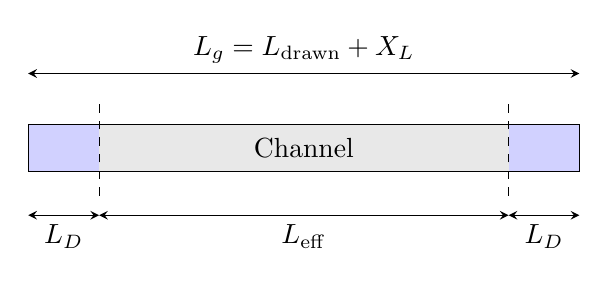
\begin{tikzpicture}[x=1cm,y=1cm,>=stealth]
\fill[gray!18] (0,0) rectangle (7,0.6);
\fill[blue!18] (0,0) rectangle (0.9,0.6);
\fill[blue!18] (6.1,0) rectangle (7,0.6);
\draw (0,0) rectangle (7,0.6);
\draw[dashed] (0.9,-0.3)--(0.9,0.9);
\draw[dashed] (6.1,-0.3)--(6.1,0.9);
\draw[<->] (0,1.25)--(7,1.25)
 node[midway,above] {\(L_g=L_{\mathrm{drawn}}+X_L\)};
\draw[<->] (0,-0.55)--(0.9,-0.55) node[midway,below] {\(L_D\)};
\draw[<->] (0.9,-0.55)--(6.1,-0.55)
 node[midway,below] {\(L_{\mathrm{eff}}\)};
\draw[<->] (6.1,-0.55)--(7,-0.55) node[midway,below] {\(L_D\)};
\node at (3.5,0.3) {Channel};
\end{tikzpicture}
\end{latin}
\caption{طرح آموزشی سهم نفوذ جانبی از دو سمت در طول مؤثر.
ابعاد شکل مقیاس فیزیکی ندارند.}
\label{fig:geometry-length}
\end{figure}

در بخش \ref{sec:clm}، نماد \(L_d\) با زیرنویس کوچک برای پیشروی
ناحیه تخلیه سمت درین در اثر بایاس به کار رفت. نماد \(L_D\) در این
بخش به نفوذ جانبی ناشی از ساخت مربوط است. هنگام ترکیب مدل‌ها، مرجع
طول و اصلاح بایاس را مشخص کنید تا یک کاهش طول دوبار وارد نشود.
در مدل \lr{CLM} ساده، \(\lambda\) اثر بایاس را در ضریب جریان
نمایش می‌دهد.

\subsubsection*{مثال آموزشی دوبرابرکردن طول و عرض ترسیم‌شده}
فرض کنید تمام ابعاد زیر برحسب نانومتر باشند و
\(X_L=X_W=-\qty{4}{\nano\metre}\)،
\(L_D=W_D=\qty{3}{\nano\metre}\).
برای افزاره مبنا با
\(L_{\mathrm{drawn}}=\qty{60}{\nano\metre}\) و
\(W_{\mathrm{drawn}}=\qty{120}{\nano\metre}\)، داریم
\[
 \begin{aligned}
 L_{\mathrm{eff}}&=60-4-2(3)=\qty{50}{\nano\metre},\\
 W_{\mathrm{eff}}&=120-4-2(3)=\qty{110}{\nano\metre}.
 \end{aligned}
\]
دوبرابرکردن طول ترسیم‌شده، طول مؤثر را به
\(120-4-6=\qty{110}{\nano\metre}\) می‌رساند. نسبت طول‌های مؤثر
\(110/50=2.2\) است. به همین ترتیب، دوبرابرکردن عرض ترسیم‌شده،
عرض مؤثر را \(\qty{230}{\nano\metre}\) می‌کند و نسبت عرض‌ها
\(230/110\approx2.091\) می‌شود.

برای محاسبه اثر هندسه به‌تنهایی، به‌طور آموزشی
\(k'=\mu C_{\mathrm{ox}}=\qty{200}{\micro\ampere\per\volt\squared}\)
و \(C_{\mathrm{ox}}=\qty{20}{\femto\farad\per\micro\metre\squared}\)
را ثابت فرض می‌کنیم. در تقریب مساحت مستطیلی کانال،
\begin{equation}
 \beta=k'\frac{W_{\mathrm{eff}}}{L_{\mathrm{eff}}},\qquad
 C_0=C_{\mathrm{ox}}W_{\mathrm{eff}}L_{\mathrm{eff}}.
 \label{eq:geometry-beta-capacitance}
\end{equation}
کمیت \(C_0\) مقیاس ظرفیت ذاتی گیت است. ظرفیت مؤثر هر پایانه به
ناحیه کاری و تقسیم بار وابسته است و ظرفیت‌های هم‌پوشانی و پیوند
نیز جداگانه مطرح‌اند. جدول \ref{tab:geometry-results} این محاسبه
هندسی را نشان می‌دهد.
\begin{table}[!htbp]
\centering
\small
\caption{نتایج هندسه فرضی با پارامترهای ماده ثابت.
طول‌ها برحسب \(\unit{\nano\metre}\) هستند.}
\label{tab:geometry-results}
\begin{tabularx}{\linewidth}{>{\raggedleft\arraybackslash}Xcccc}
\toprule
حالت & \(L_{\mathrm{eff}}\) & \(W_{\mathrm{eff}}\) &
\(\beta\)، \(\unit{\micro\ampere\per\volt\squared}\) &
\(C_0\)، \(\unit{\femto\farad}\)\\
\midrule
مبنا & \num{50} & \num{110} & \num{440} & \num{0.110}\\
طول ترسیم‌شده دوبرابر & \num{110} & \num{110} & \num{200} & \num{0.242}\\
عرض ترسیم‌شده دوبرابر & \num{50} & \num{230} & \num{920} & \num{0.230}\\
\bottomrule
\end{tabularx}
\end{table}
برای نمونه، \(\qty{50}{\nano\metre}=\qty{0.05}{\micro\metre}\)
و \(\qty{110}{\nano\metre}=\qty{0.11}{\micro\metre}\)، پس
مساحت مبنا \(\qty{0.0055}{\micro\metre\squared}\) است و
\(C_0=20(0.0055)=\qty{0.11}{\femto\farad}\) می‌شود.
در مدل مربعی با آستانه و بایاس ثابت، نسبت جریان برای تغییر طول
\(200/440\approx0.4545\) و برای تغییر عرض
\(920/440\approx2.091\) است.

در افزاره واقعی، هندسه می‌تواند آستانه را از راه اثر کانال کوتاه
و باریک نیز تغییر دهد. همچنین تغییر طول بر \lr{CLM} و
\lr{Velocity Saturation} اثر می‌گذارد. بنابراین، برای پیش‌بینی
جریان باید همه پارامترهای وابسته به هندسه را به‌روز کرد.
اسلاید ۳۶ افزایش آستانه و کاهش \lr{CLM} در کانال بلندتر را برای
روندهای مورد بحث دوره بیان می‌کند. نتیجه ساده \(I\propto1/L\)
به فرض ثابت‌بودن پارامترهای دیگر وابسته است
\cite[صفحه ۸۶]{weste}\cite[اسلاید ۳۶]{nonideal}.

\subsubsection*{هندسه یکسان و \lr{Matching}}
وقتی برابری یا نسبت دقیق جریان مهم است، کتاب استفاده از افزاره‌های
با طول و عرض یکسان را پیشنهاد می‌کند. برای نسبت‌های صحیح می‌توان
چند افزاره واحد یکسان را موازی کرد. مثلاً سه واحد موازی با بایاس‌های
پایانه‌ای یکسان، در مدل افزاره‌های یکسان سه برابر یک واحد جریان دارند.
هر واحد، همان اصلاح هندسی و آستانه واحد مبنا را تجربه می‌کند.

جهت‌گیری و محیط اطراف نیز بر ساخت اثر دارند. مرجع برای نمونه‌های
فرایندی کوچک‌تر از \(\qty{0.25}{\micro\metre}\)، اهمیت جهت‌گیری را
ذکر می‌کند. مقدار \lr{Polysilicon} مجاور می‌تواند سرعت حکاکی را
عوض کند. جهت‌گیری مشترک و \lr{Dummy Polysilicon} به یکنواختی محیط
کمک می‌کنند. چیدمان \lr{Interdigitated} یعنی درهم‌گذاری واحدهای
دو گروه، مانند ترتیب \lr{ABAB}، تا گروه‌ها محیط مکانی مشابه‌تری
ببینند. کتاب استفاده از آن را در صورت امکان مطرح می‌کند
\cite[صفحات ۸۶ و ۸۷]{weste}. انتخاب چیدمان واقعی تابع قواعد همان
فرایند و نوع خطای مورد کنترل است.

\subsubsection*{مکمل اسلایدها درباره \lr{PVT} و \lr{Process Corners}}
\label{sec:pvt-supplement}
اسلایدهای ۳۱ تا ۳۴، تغییر پارامترهای ساخت، تغذیه و دما را نیز
معرفی می‌کنند \cite{nonideal}. عبارت \lr{PVT} مخفف
\lr{Process, Voltage, Temperature} است. طول مؤثر، آستانه و ضخامت
عایق، مقادیر قطعی یکسان برای همه تراشه‌ها ندارند. تغذیه و دما نیز
در زمان و مکان تغییر می‌کنند. \lr{Corner} مجموعه‌ای مشخص از شرایط
مدل برای بررسی رفتار مدار است.

در قرارداد اسلایدها، \lr{T} به معنی \lr{Typical}، \lr{F} به معنی
\lr{Fast} و \lr{S} به معنی \lr{Slow} است. در مثال فرایندی اسلاید
۳۱، طول کوتاه‌تر، آستانه کمتر و عایق نازک‌تر به جریان قوی‌تر و
رفتار سریع‌تر کمک می‌کنند. پارامترهای \lr{nMOS} و \lr{pMOS} کاملاً
مستقل نیستند. دو حرف \lr{FS} یعنی \lr{nMOS} سریع و \lr{pMOS} کند،
و \lr{SF} حالت معکوس آن است. \lr{TT}، \lr{FF} و \lr{SS} نیز
به‌ترتیب حالت معمول و دو حالت هم‌جهت را نمایش می‌دهند.

اسلاید ۳۳ برای توصیف کامل‌تر، چهار حرف را به ترتیب
\lr{nMOS}، \lr{pMOS}، تغذیه و دما می‌نویسد. در قرارداد معمول همان
اسلایدها، تغذیه بالاتر و دمای پایین‌تر با حرف \lr{F} همراه‌اند.
جدول \ref{tab:pvt-environment} مقادیر نمونه اسلاید ۳۲ را بازنویسی
می‌کند. این مقادیر یک مثال درسی‌اند و باید برای هر فناوری از مدل
همان فناوری استفاده کرد. حرف \lr{T} در نام \lr{Corner} به معنی
حالت معمول است. نماد ریاضی \(T\) در روابط این جزوه دمای مطلق است.
\begin{table}[!htbp]
\centering
\caption{نمونه شرایط محیطی اسلاید ۳۲.}
\label{tab:pvt-environment}
\begin{tabular}{ccc}
\toprule
حالت & تغذیه، \(\unit{\volt}\) & دما، \(\unit{\degreeCelsius}\)\\
\midrule
\lr{F} & \num{1.98} & \num{0}\\
\lr{T} & \num{1.8} & \num{70}\\
\lr{S} & \num{1.62} & \num{125}\\
\bottomrule
\end{tabular}
\end{table}

در اسلاید ۳۴، مثال \lr{SSSS} برای بررسی زمان چرخه، \lr{FFFF}
برای توان و \lr{FFFS} برای نشتی زیرآستانه آمده است. برای نمونه،
\lr{FFFS} یعنی هر دو نوع ترانزیستور سریع، تغذیه بالا و دمای بالا.
آخرین حرف \lr{S} در اینجا همان دمای بالای جدول است.
گوشه توان \lr{FFFF} باید با مؤلفه توان مورد بررسی تفسیر شود.
توان دینامیکی از ظرفیت سوئیچ‌شونده، فعالیت، فرکانس و تغذیه اثر
می‌گیرد و توان نشتی نیز وابستگی دمایی خود را دارد. بنابراین، تعیین
بیشینه توان کل به مجموع مؤلفه‌ها و شرایط کار نیاز دارد.

حساسیت دمایی جریان در تغذیه پایین می‌تواند علامت عوض کند، چنان‌که
در \eqref{eq:temperature-coefficient} دیدیم. برای تعیین بدترین
تأخیر، باید دماهای مربوط به مدل بررسی شوند. همچنین بررسی
\lr{Corner}‌ها شواهدی درباره شرایط مدل‌شده فراهم می‌کند. پراکندگی
محلی و \lr{Mismatch} به مدل آماری مناسب خود نیاز دارند. این مکمل،
معنای قراردادهای اسلاید را برای خواندن تحلیل مدار روشن می‌کند.

% !TeX root = booklet-02.tex
\clearpage
\subsection{جمع‌بندی اثرهای غیرایده‌آل و کاربرد در مدار}
\label{sec:nonideal-summary}
بخش \secnum{۲.۴.۷} کتاب، نتیجه بحث را در پنج موضوع مدار جمع می‌کند
\cite[صفحات ۸۶ و ۸۷]{weste}. اسلاید ۳۰ نیز انتخاب تغذیه،
\lr{Logical Effort}، توان سکون، \lr{Pass Transistor} و دمای کار را
از کاربردهای این اثرها می‌شمارد \cite{nonideal}.

\subsubsection*{افت آستانه در عبور سطح منطقی}
وقتی \lr{nMOS} با گیت \(V_{DD}\) یک گره را به سمت سطح بالا شارژ
می‌کند، افزایش ولتاژ گره، \(V_{GS}\) را کاهش می‌دهد. در تقریب
آستانه ثابت، جریان هدایت قوی نزدیک
\(V_{\mathrm{out}}=V_{DD}-V_{tn}\) ضعیف می‌شود. در \lr{pMOS} که
سطح پایین را عبور می‌دهد، حد متناظر حدود \(|V_{tp}|\) بالای زمین
است. \lr{Body Effect} بزرگی افت آستانه را بیشتر می‌کند. وقتی آستانه
سهم بزرگی از تغذیه باشد، این افت برای سطح منطقی اهمیت بیشتری دارد.
در \lr{Transmission Gate}، یک \lr{nMOS} و یک \lr{pMOS} با کنترل
مکمل به‌صورت موازی قرار می‌گیرند. \lr{nMOS} عبور سطح پایین و
\lr{pMOS} عبور سطح بالا را تقویت می‌کند
\cite[بخش \secnum{۲.۴.۷}]{weste}. استخراج مشخصه انتقال و سطوح
منطقی این مدارها در بخش \secnum{۲.۵}، موضوع جزوه سوم است.

\subsubsection*{نشتی، توان سکون و نگهداری داده}
در \lr{Static CMOS} ایده‌آل، در حالت ماندگار مسیر هدایت بین تغذیه
و زمین قطع است. مدل واقعی مسیرهای نشتی بخش \ref{sec:leakage} را
دارد. در صورت تغذیه واحد و با قرارداد جریان مثبت دریافتی از منبع،
توان ماندگار \(P_{\mathrm{static}}=V_{DD}I_{DD}\) است.
برای چند منبع، سهم هر منبع از حاصل‌ضرب ولتاژ و جریان همان منبع
محاسبه می‌شود. جریان‌های شاخه‌ای باید با \lr{KCL} به جریان منبع
تبدیل شوند.

در گره‌ای که داده را به شکل بار ذخیره می‌کند، نشتی بار را جابه‌جا
می‌کند و ولتاژ گره تغییر می‌کند. برای ظرفیت ثابت،
\(\Delta Q=C\Delta V\) است. اگر جریان نشتی را در یک بازه تقریباً
ثابت فرض کنیم، \(|\Delta Q|\approx|I_{\mathrm{leak}}|\Delta t\)
و زمان رسیدن به تغییر ولتاژ مجاز تقریباً برابر می‌شود با
\begin{equation}
 \Delta t\approx\frac{C|\Delta V|}{|I_{\mathrm{leak}}|}.
 \label{eq:retention-time-estimate}
\end{equation}
واحد \(\mathrm{F}\,\mathrm{V}/\mathrm{A}=\mathrm{s}\) است.
این برآورد به ثابت‌بودن تقریبی ظرفیت و جریان تکیه دارد. در حالت
کلی، تغییر ولتاژ با جریان وابسته به ولتاژ و دما محاسبه می‌شود.
کتاب نیاز به \lr{Feedback} یا تجدید داده در ساختارهای ذخیره‌ساز را
از پیامدهای نشتی مطرح می‌کند. آستانه پایین، جریان روشن و سرعت را
تقویت می‌کند و آستانه بالا نشتی را کاهش می‌دهد. فرایندهای دارای
چند انتخاب آستانه از این وابستگی برای مسیرهای با نیازهای متفاوت
استفاده می‌کنند \cite[صفحه ۸۷]{weste}.

در روایت فناوری مرجع، نازک‌شدن عایق، نشتی تونلی گیت را مهم کرده
و استفاده از عایق‌های \lr{High-k} را برانگیخته است. همچنین شیب
زیرآستانه در نمونه‌های بحث کتاب در حدود
\(\qty{60}{\milli\volt}\) تا \(\qty{100}{\milli\volt}\) به ازای هر
دهه تغییر جریان است. رابطه \eqref{eq:leakage-subthreshold-slope}
وابستگی آن را به \(n\) و دما نشان می‌دهد
\cite[صفحات ۸۲ و ۸۷]{weste}.

\subsubsection*{انتخاب \lr{VDD} و بازده کاهش‌یابنده افزایش ولتاژ}
در مدل مربعی، جریان اشباع با مربع اضافه‌ولتاژ رشد می‌کند. با
\lr{Mobility Degradation} و \lr{Velocity Saturation}، رشد جریان
در بایاس بالا کندتر می‌شود. در نتیجه، افزایش تغذیه با بهبود جریان
کمتری نسبت به پیش‌بینی ساده مربعی همراه است. هم‌زمان، انرژی
سوئیچ‌کردن ظرفیت با \(V_{DD}^2\) رشد می‌کند. تنش عایق نازک و
کانال کوتاه نیز محدوده مجاز ولتاژ را محدود می‌کند
\cite[صفحه ۸۷]{weste}. مقدار مجاز ولتاژ و شرایط قابلیت اطمینان از
اطلاعات همان فناوری تعیین می‌شوند.

\subsubsection*{ترانزیستورهای سری، جریان و تأخیر}
در ساختار سری، ولتاژ کل بین چند افزاره تقسیم می‌شود. کاهش میدان
هر افزاره می‌تواند اثر \lr{Velocity Saturation} را کم کند. کتاب
بیان می‌کند که جریان دو \lr{nMOS} سری می‌تواند از نصف جریان یک
\lr{nMOS} با همان عرض و طول بیشتر باشد. این اثر برای \lr{nMOS}
با \lr{Mobility} بالاتر محسوس‌تر است
\cite[صفحه ۸۷]{weste}. در برآورد
\(t\approx C\Delta V/I\)، جریان بیشتر به زمان کوتاه‌تر برای
جابه‌جایی همان بار کمک می‌کند. مدل دقیق تأخیر به تغییر جریان و
ظرفیت طی گذار وابسته است.

تمرین‌های \secnum{۲.۲} و \secnum{۲.۳}، ساختار سری را با یک ترانزیستور طول \(2L\)
مقایسه می‌کنند. مثال آموزشی بخش \ref{sec:series-velocity-example}
مقایسه کتاب در جمع‌بندی را با یک ترانزیستور طول \(L\) انجام می‌دهد.
مشخص‌کردن افزاره مرجع و مدل، برای تفسیر نسبت جریان ضروری است.

\subsubsection*{تطبیق جریان و \lr{Matching}}
برای برابری رفتار، ابعاد، جهت‌گیری و محیط ساخت افزاره‌ها باید تا
حد امکان مشابه باشند. واحدهای موازی یکسان و درهم‌گذاری مناسب
می‌توانند به ساخت نسبت جریان کمک کنند. مثال بخش
\ref{sec:geometry-dependence} نشان داد که یک نسبت در ابعاد
ترسیم‌شده الزاماً همان نسبت را در ابعاد مؤثر ایجاد نمی‌کند
\cite[صفحات ۸۶ و ۸۷]{weste}.

\subsubsection*{مثال آموزشی جریان دو افزاره سری در مدل سرعت}
\label{sec:series-velocity-example}
دو \lr{nMOS} یکسان با گیت مشترک \(V_{DD}=\qty{1}{\volt}\)،
سورس پایین در زمین و درین بالا در \(\qty{1}{\volt}\) را در نظر
بگیرید. برای هر واحد فرض کنید
\(V_t=\qty{0.3}{\volt}\)، \(V_c=\qty{1}{\volt}\) و
\(\beta=\qty{400}{\micro\ampere\per\volt\squared}\) باشند.
اثر بدنه، \lr{DIBL} و \lr{CLM} در این مثال آموزشی حذف شده‌اند.
ولتاژ گره میانی را \(x\) می‌نامیم.
رابطه‌های \eqref{eq:high-field-linear} و
\eqref{eq:current-reduction-factor} را برای هر افزاره جداگانه به
کار می‌بریم. برای اختصار، اگر \(a=V_{GS}-V_t>0\) و \(d=V_{DS}\)
باشند، تابع جریان همین مدل را می‌نویسیم
\begin{equation}
 J(a,d)=
 \begin{cases}
 \displaystyle\beta\frac{ad-d^2/2}{1+d/V_c},
       &0\le d<\dfrac{aV_c}{a+V_c},\\[6pt]
 \displaystyle\frac{\beta a^2}{2(1+a/V_c)},
       &d\ge\dfrac{aV_c}{a+V_c}.
 \end{cases}
 \label{eq:series-velocity-function}
\end{equation}
برای افزاره پایین، \(a=0.7\) و \(d=x\) برحسب ولت‌اند.
برای افزاره بالا، \(a=0.7-x\) و \(d=1-x\) هستند. شرط برابری
جریان‌ها در گره میانی می‌شود
\begin{equation}
 J(0.7,x)=J(0.7-x,1-x).
 \label{eq:series-velocity-kcl}
\end{equation}
تابع‌ها با ولتاژ برحسب ولت و ضریب \(\beta\) داده‌شده ارزیابی
می‌شوند. ابتدا \(0<x<0.7\) را انتخاب می‌کنیم تا هر دو افزاره
روشن باشند. در \(x=\qty{0.1}{\volt}\)، جریان پایین
\(\qty{23.64}{\micro\ampere}\) و جریان بالا
\(\qty{45.00}{\micro\ampere}\) است. پس باید \(x\) افزایش یابد.
در \(x=\qty{0.2}{\volt}\)، این جریان‌ها به‌ترتیب
\(\qty{40.00}{\micro\ampere}\) و
\(\qty{33.33}{\micro\ampere}\) هستند. ریشه میان این دو مقدار است.
با نصف‌کردن مکرر بازه و انتخاب نیمه‌ای که اختلاف جریان در دو سر
آن تغییر علامت می‌دهد، نتیجه چنین به دست می‌آید
\begin{equation}
 x\approx\qty{0.17370}{\volt},\qquad
 I_{\mathrm{series}}\approx\qty{36.296}{\micro\ampere}.
 \label{eq:series-velocity-result}
\end{equation}
کنترل ناحیه کاری ضروری است. برای افزاره پایین، مرز اشباع
\(0.7/(1+0.7)\approx\qty{0.41176}{\volt}\) است و
\(x\) از آن کمتر است، پس شاخه \lr{Linear} انتخاب می‌شود.
برای افزاره بالا، اضافه‌ولتاژ
\(\qty{0.52630}{\volt}\)، ولتاژ درین و سورس
\(\qty{0.82630}{\volt}\) و مرز اشباع
\(\qty{0.34482}{\volt}\) است. پس افزاره بالا در اشباع است.

یک افزاره واحد طول \(L\) در همان بایاس کل، در اشباع قرار دارد و
جریان آن برابر است با
\begin{equation}
 I_{\mathrm{single}}=
 \frac{(400/2)(0.7)^2}{1+0.7/1}\,\unit{\micro\ampere}
 \approx\qty{57.647}{\micro\ampere}.
 \label{eq:series-velocity-reference}
\end{equation}
بنابراین، \(I_{\mathrm{series}}/I_{\mathrm{single}}\approx0.6296\)
است که از نصف بزرگ‌تر است. این مقدار، نتیجه پارامترها و فرض‌های
همین مثال است. برای افزودن اثر بدنه، باید آستانه افزاره بالا را
تابع \(x\) کرد و برابری جریان‌ها را دوباره حل کرد.

\subsubsection*{تمرین آموزشی نگهداری بار و پاسخ}
گرهی با ظرفیت ثابت \(\qty{10}{\femto\farad}\)، جریان نشتی تقریباً
ثابت \(\qty{1}{\nano\ampere}\) و تغییر ولتاژ مجاز
\(\qty{0.1}{\volt}\) فرض کنید. زمان برآوردی نگهداری بار چقدر است؟
با تبدیل واحدها و استفاده از \eqref{eq:retention-time-estimate}، زمان
برآوردی به دست می‌آید.
\[
 \Delta t=\frac{(10\times10^{-15})(0.1)}{10^{-9}}
 =\qty{1e-6}{\second}=\qty{1}{\micro\second}.
\]
اگر جریان در همان شرایط دو برابر شود و ظرفیت و حاشیه ولتاژ ثابت
بمانند، زمان به \(\qty{0.5}{\micro\second}\) کاهش می‌یابد.
برای نمونه واقعی با جریان متغیر، معادله تغییر بار باید با مدل
جریان همان گره حل شود.

\subsubsection*{راهنمای نهایی حل و نقشه پوشش منابع}
پیش از جای‌گذاری عددها، بایاس‌های پایانه‌ای، مدل مسئله و شرایط ثابت
را تعیین کنید. ابعاد مؤثر را با قرارداد مدل به کار ببرید. آستانه
متناسب با بدنه، درین، هندسه و دما را محاسبه کنید. سپس اضافه‌ولتاژ
و مرز ناحیه کاری را به دست آورید. در مدار چندترانزیستوری، ولتاژ
گره‌های داخلی از \lr{KCL} تعیین می‌شود. پس از حل، ناحیه کاری،
ریشه فیزیکی، واحدها، رفتار حدی و دامنه تقریب‌ها را بررسی کنید.
پارامترهای تجربی چند مدل باید با قرارداد یکسان ترکیب شوند.

جدول \ref{tab:booklet-two-coverage} مسیر بازگشت از موضوع به کتاب و
اسلاید را نشان می‌دهد. شماره‌های رابطه این جزوه مستقل از کتاب‌اند.
\begin{table}[!htbp]
\centering
\small
\caption{نقشه موضوعی بخش \secnum{۲.۴} کتاب و اسلایدهای \lr{Nonideal Transistor Theory}.}
\label{tab:booklet-two-coverage}
\begin{tabularx}{\linewidth}{c>{\raggedleft\arraybackslash}Xc}
\toprule
بخش کتاب & موضوع در همین جزوه & اسلاید\\
\midrule
\secnum{۲.۴.۱} & بخش \ref{sec:high-field}، میدان، سرعت و مدل توان & ۶ تا ۱۲\\
\secnum{۲.۴.۲} & بخش \ref{sec:clm}، \lr{CLM} و شیب خروجی & ۱۳ و ۱۴\\
\secnum{۲.۴.۳} & بخش \ref{sec:threshold-effects}، اثرهای آستانه & ۱۵ تا ۲۰\\
\secnum{۲.۴.۴} & بخش \ref{sec:leakage}، سه مسیر نشتی & ۲۱ تا ۲۸\\
\secnum{۲.۴.۵} & بخش \ref{sec:temperature-dependence}، رقابت اثرهای دما & ۲۹\\
\secnum{۲.۴.۶} & بخش \ref{sec:geometry-dependence}، ابعاد مؤثر و تطبیق & ۳۵ و ۳۶\\
\secnum{۲.۴.۷} & بخش \ref{sec:nonideal-summary}، پیامدهای مداری & ۳۰\\
مکمل دوره & \hyperref[sec:pvt-supplement]{مکمل \lr{PVT} و قراردادهای \lr{Corner}} & ۳۱ تا ۳۴\\
\bottomrule
\end{tabularx}
\end{table}

اسلایدهای ۳ تا ۵ مقدمه و مرور منحنی‌ها هستند و موضوع آن‌ها در مرور
پیش‌نیازها و آغاز بخش \ref{sec:nonideal-current} آمده است.
فهرست اسلاید ۳۷ با هفت تمرین سری نخست فصل دوم مطابقت دارد.
اثبات تمرین \secnum{۲.۶} در بخش \ref{sec:high-field}، حل \secnum{۲.۲} در بازسازی
مرجع مدار سری و حل \secnum{۲.۳} و \secnum{۲.۷} تا \secnum{۲.۹} در فصل تمرین‌های اثر آستانه
آمده است. فصل پایانی تمرین‌ها، مسئله \secnum{۲.۱۰} را با مقایسه مدل مربعی
و نشتی زیرآستانه حل می‌کند. این ترتیب، پیش‌نیاز هر تمرین را پیش از
حل آن فراهم می‌کند.

\BookletReview{notes/booklet-02/review-high-field}
\BookletReview{notes/booklet-02/threshold-exercises}
\BookletReview{notes/booklet-02/leakage-exercises}

% !TeX root = booklet-03.tex
\BookletReview{notes/booklet-03/prerequisites}
\ifCompleteNotes\else
\setcounter{chapter}{1}
\chapter{مشخصه انتقال ولتاژ در مدارهای منطقی}
\fi
\setcounter{section}{4}
\section{مشخصه انتقال \lr{DC}}
\label{sec:dc-transfer}
در \lr{DC Transfer Characteristic}، برای هر ولتاژ ورودی، خروجی
مدار را پس از رسیدن به حالت ماندگار تعیین می‌کنیم. فرض می‌شود
ورودی آن‌قدر آهسته تغییر می‌کند که ظرفیت‌ها فرصت شارژ و تخلیه
داشته باشند. مدار دیجیتال نیز از ولتاژها و جریان‌های پیوسته
ساخته شده است. تفسیر منطقی، بازه‌هایی از این ولتاژها را به صفر
و یک نسبت می‌دهد \cite[مقدمه بخش \secnum{۲.۵}، صفحه ۸۷]{weste}.
% !TeX root = booklet-03.tex
\subsection{مشخصه \lr{DC} یک \lr{Static CMOS Inverter}}
\label{sec:inverter-dc}
هدف این بخش، محاسبه \(V_{\mathrm{out}}\) برای هر
\(V_{\mathrm{in}}\) است. مبنای مدار و تقسیم‌بندی، بخش
\secnum{۲.۵.۱} کتاب و اسلایدهای ۳ تا ۷ است
\cite{weste,dcslides}. ابتدا قراردادهای عمومی ولتاژ و جریان را
می‌نویسیم. استخراج پنج ناحیه با مدل متقارن کتاب انجام می‌شود.

\subsubsection{مدار، فرض‌ها و قرارداد علامت}
\label{sec:inverter-conventions}
در شکل \ref{fig:inverter-circuit}، سورس \lr{nMOS} به زمین و سورس
\lr{pMOS} به \(V_{DD}\) متصل است. گیت‌ها به یک ورودی و درین‌ها
به یک خروجی وصل‌اند. بدنه \lr{nMOS} را به زمین و بدنه
\lr{pMOS} را به تغذیه می‌بندیم. پس اختلاف ولتاژ سورس و بدنه برای
هر دو صفر است و تغییر آستانه ناشی از بایاس بدنه در این مدار ایجاد
نمی‌شود. فرض می‌کنیم \(0\le V_{\mathrm{in}},V_{\mathrm{out}}\le V_{DD}\).
\begin{figure}[!htbp]
\centering
\begin{latin}
\PersianMathDigits
\begin{circuitikz}[scale=1,transform shape]
\draw (3,1.3) node[nmos] (n) {};
\draw (3,3.7) node[pmos] (p) {};
\draw (n.S)--(3,0.3) node[ground] {};
\draw (p.S)--(3,4.7) node[ocirc] {} node[above] {\(V_{DD}\)};
\draw (n.D)--(p.D);
\draw (n.G)--(1.3,1.3)--(1.3,3.7)--(p.G);
\draw (1.3,2.5) node[circ] {}--(0.4,2.5) node[ocirc] {}
 node[left] {\(V_{\mathrm{in}}\)};
\draw (3,2.5) node[circ] {}--(5,2.5) node[ocirc] {}
 node[right] {\(V_{\mathrm{out}}\)};
\draw[->] (4.8,4.2)--(4.8,3.3) node[midway,right] {\(I_p\)};
\draw[->] (4.8,1.8)--(4.8,0.9) node[midway,right] {\(I_n\)};
\node[right] at (3.3,3.7) {pMOS};
\node[right] at (3.3,1.3) {nMOS};
\end{circuitikz}
\end{latin}
\caption{بازترسیم آموزشی مدار شکل \secnum{۲.۲۵} کتاب و اسلاید ۳.
پیکان‌ها بزرگی جریان‌های بالاکش و پایین‌کش را نشان می‌دهند.
بدنه‌ها به سورس‌های متناظر متصل‌اند.}
\label{fig:inverter-circuit}
\end{figure}

با تعریف اختلاف ولتاژ پایانه‌ها، روابط \lr{nMOS} چنین‌اند
\begin{equation}
 V_{GS,n}=V_{\mathrm{in}},\qquad
 V_{DS,n}=V_{\mathrm{out}}.
 \label{eq:inverter-n-voltages}
\end{equation}
برای \lr{pMOS}، قرارداد علامت‌دار کتاب و قرارداد بزرگی مثبت به‌ترتیب
به صورت زیر به هم مربوط‌اند
\begin{align}
 V_{GS,p}&=V_{\mathrm{in}}-V_{DD},&
 V_{DS,p}&=V_{\mathrm{out}}-V_{DD},
 \label{eq:inverter-p-signed}\\
 V_{SG,p}&=V_{DD}-V_{\mathrm{in}}=-V_{GS,p},&
 V_{SD,p}&=V_{DD}-V_{\mathrm{out}}=-V_{DS,p}.
 \label{eq:inverter-p-magnitudes}
\end{align}
آستانه \lr{nMOS} را \(V_{tn}>0\) و آستانه علامت‌دار
\lr{pMOS} را \(V_{tp}<0\) می‌نامیم. بزرگی آستانه را به صورت زیر
تعریف می‌کنیم.
\[
 V_{TP}=|V_{tp}|=-V_{tp},\qquad V_{TP}>0.
\]
برای جریان نیز
\(I_n=I_{DS,n}\ge0\) و \(I_p=|I_{DS,p}|\ge0\) به کار می‌روند.
با جهت جریان درین به سورس، \(I_{DS,p}=-I_p\) است.

خروجی را بدون جریان بار \lr{DC} فرض می‌کنیم. در حالت ماندگار،
\lr{KCL} به رابطه اصلی تحلیل می‌انجامد
\begin{equation}
 \boxed{I_n(V_{\mathrm{in}},V_{\mathrm{out}})
       =I_p(V_{\mathrm{in}},V_{\mathrm{out}})}.
 \label{eq:inverter-kcl}
\end{equation}
جریان تغذیه در این مدل همان \(I_{DD}=I_p=I_n\) است. وجود ظرفیت
خروجی با این شرط ماندگار سازگار است. اگر بار جریان ثابت یا مقاومتی
داشته باشد، باید \(I_L\) را در معادله گره وارد کرد.

برای استخراج اصلی، فرض‌های متقارن کتاب را به کار می‌بریم
\begin{equation}
 V_{tn}=V_{TP}=V_t>0,\qquad
 \beta_n=\beta_p=\beta>0,\qquad V_{DD}>2V_t.
 \label{eq:inverter-symmetry}
\end{equation}
مدل، \lr{Long-channel Shockley} با آستانه و \lr{Mobility} ثابت است.
در استخراج ایده‌آل، \lr{CLM} و نشتی صفر فرض می‌شوند. شرط آخر،
بازه‌ای برای روشن‌بودن هم‌زمان دو افزاره ایجاد می‌کند. اگر تغذیه
از مجموع بزرگی دو آستانه کمتر باشد، ترتیب پنج‌ناحیه‌ای حاضر
نیازمند بازنگری است و جریان زیرآستانه نیز می‌تواند تعیین‌کننده شود.

پارامتر \(\beta\) با واحد \(\unit{\ampere\per\volt\squared}\)
از \(\beta=\mu C_{\mathrm{ox}}W/L\) به دست می‌آید. با
\(C_{\mathrm{ox}}\) و طول یکسان، برابری دو \(\beta\) نیازمند
\(\mu_nW_n=\mu_pW_p\) است. کتاب برای جبران \lr{Mobility}
کمتر حفره‌ها، عرض \lr{pMOS} حدود دو تا سه برابر \lr{nMOS} را در
تقریب این بخش مطرح می‌کند \cite[صفحه ۸۸]{weste}. این نسبت،
تقریب همان بحث است و مقدار دقیق به فناوری و بایاس وابسته است.

\subsubsection{مدل جریان و تبدیل شرط‌های ناحیه کاری}
\label{sec:inverter-regions}
برای خوانایی روابط، اضافه‌ولتاژهای مثبت را تعریف می‌کنیم
\begin{equation}
 a=V_{\mathrm{in}}-V_{tn},\qquad
 b=V_{DD}-V_{\mathrm{in}}-V_{TP},\qquad
 y=V_{\mathrm{out}},\qquad u=V_{DD}-y.
 \label{eq:inverter-ab-definitions}
\end{equation}
کمیت \(u\) افت ولتاژ سورس به درین \lr{pMOS} است. نمادهای
\(a,b\) با واحد ولت‌اند و تنها وقتی مثبت باشند افزاره متناظر
در مدل هدایت قوی روشن است. روابط جریان مدل مربعی کتاب با این
نمادها چنین نوشته می‌شوند
\begin{equation}
 I_n=
 \begin{cases}
 0,&a\le0,\\[2pt]
 \beta_n(ay-y^2/2),&a>0,\quad 0\le y<a,\\[2pt]
 \beta_n a^2/2,&a>0,\quad y\ge a,
 \end{cases}
 \label{eq:inverter-n-current}
\end{equation}
و برای بزرگی جریان \lr{pMOS} داریم
\begin{equation}
 I_p=
 \begin{cases}
 0,&b\le0,\\[2pt]
 \beta_p(bu-u^2/2),&b>0,\quad 0\le u<b,\\[2pt]
 \beta_p b^2/2,&b>0,\quad u\ge b.
 \end{cases}
 \label{eq:inverter-p-current}
\end{equation}
این روابط از مدل بخش \secnum{۲.۲} کتاب با قراردادهای جدول
\secnum{۲.۲} به دست آمده‌اند \cite[صفحات ۶۶ و ۸۸]{weste}.
در مرز \(y=a\) یا \(u=b\)، دو شاخه روشن، جریان یکسانی می‌دهند.
برای نمونه، \(\beta_n[a(a)-a^2/2]=\beta_na^2/2\).
نسبت‌دادن نقطه مرزی به شاخه اشباع، قرارداد این جزوه است.
در آستانه دقیق، جریان ایده‌آل صفر است.

برای \lr{nMOS} روشن، شرط اشباع
\(V_{DS,n}\ge V_{GS,n}-V_{tn}\) مستقیماً می‌دهد
\(y\ge V_{\mathrm{in}}-V_{tn}\).
برای \lr{pMOS} روشن، از بزرگی ولتاژها شروع می‌کنیم
\begin{align}
 V_{SD,p}&\ge V_{SG,p}-V_{TP},\notag\\
 V_{DD}-y&\ge V_{DD}-V_{\mathrm{in}}-V_{TP},\notag\\
 -y&\ge -V_{\mathrm{in}}-V_{TP},\notag\\
 \boxed{y\le V_{\mathrm{in}}+V_{TP}}.
 \label{eq:inverter-p-saturation-condition}
\end{align}
در مرحله آخر، ضرب در منفی یک، جهت نامساوی را عوض کرده است.
با \(V_{TP}=-V_{tp}\)، این شرط برابر
\(y\le V_{\mathrm{in}}-V_{tp}\) در قرارداد کتاب است.
جدول \ref{tab:inverter-device-regions} همه شرط‌ها را جمع می‌کند
\cite[جدول \secnum{۲.۲}]{weste}\cite[اسلایدهای ۵ و ۶]{dcslides}.
\begin{table}[!htbp]
\centering
\small
\caption{شرط‌های ناحیه کاری در مختصات ورودی و خروجی.
در ردیف‌های روشن، شرط روشن‌بودن نیز باید برقرار باشد.}
\label{tab:inverter-device-regions}
\begin{tabularx}{\linewidth}{cc>{\raggedleft\arraybackslash}X}
\toprule
افزاره & ناحیه & شرط\\
\midrule
\lr{nMOS} & \lr{Cutoff} & \(V_{\mathrm{in}}\le V_{tn}\)\\
\lr{nMOS} & \lr{Linear} & \(V_{\mathrm{in}}>V_{tn},\quad 0\le y<V_{\mathrm{in}}-V_{tn}\)\\
\lr{nMOS} & \lr{Saturation} & \(V_{\mathrm{in}}>V_{tn},\quad y\ge V_{\mathrm{in}}-V_{tn}\)\\
\lr{pMOS} & \lr{Cutoff} & \(V_{\mathrm{in}}\ge V_{DD}-V_{TP}\)\\
\lr{pMOS} & \lr{Linear} & \(V_{\mathrm{in}}<V_{DD}-V_{TP},\quad y>V_{\mathrm{in}}+V_{TP}\)\\
\lr{pMOS} & \lr{Saturation} & \(V_{\mathrm{in}}<V_{DD}-V_{TP},\quad y\le V_{\mathrm{in}}+V_{TP}\)\\
\bottomrule
\end{tabularx}
\end{table}

در یک ورودی مشخص، انتخاب ناحیه به خروجی مجهول هم وابسته است.
بنابراین، روش حل چنین است. یک ترکیب ناحیه را فرض می‌کنیم، جریان‌های
متناظر را برابر می‌گذاریم و خروجی را حساب می‌کنیم. سپس همه شرط‌های
آن ترکیب را با خروجی به‌دست‌آمده می‌سنجیم. اگر شرطی نقض شود،
شاخه دیگری باید بررسی شود.

\subsubsection{روش ترسیمی و تقاطع منحنی‌های جریان}
\label{sec:inverter-graphical}
در ورودی ثابت، \(a\) و \(b\) ثابت‌اند. اگر خروجی \(y\) را از
صفر تا تغذیه تغییر دهیم، جریان \lr{nMOS} ابتدا افزایش می‌یابد و
سپس در مدل ایده‌آل ثابت می‌شود. برای \lr{pMOS}، افزایش خروجی،
\(u=V_{DD}-y\) را کم می‌کند. جریان آن ابتدا می‌تواند در اشباع
ثابت باشد و سپس تا صفر کاهش یابد. نقطه تقاطع دو منحنی شرط
\eqref{eq:inverter-kcl} را برآورده می‌کند. با تکرار این کار برای
ورودی‌های مختلف، مشخصه انتقال به دست می‌آید
\cite[شکل \secnum{۲.۲۶}]{weste}.

شکل \ref{fig:inverter-current-intersection} نمونه آموزشی این ساخت
ترسیمی است. پارامترهای فرضی آن
\(V_{DD}=\qty{1.2}{\volt}\)، \(V_t=\qty{0.3}{\volt}\)،
\(\beta_n=\beta_p=\qty{200}{\micro\ampere\per\volt\squared}\)
و \(V_{\mathrm{in}}=\qty{0.5}{\volt}\) هستند.
پس \(a=\qty{0.2}{\volt}\) و \(b=\qty{0.4}{\volt}\) است.
حد جریان اشباع \lr{nMOS} برابر \(\qty{4}{\micro\ampere}\) و حد
متناظر \lr{pMOS} برابر \(\qty{16}{\micro\ampere}\) است.
تقاطع در \(y\approx\qty{1.1464}{\volt}\) و
\(I_n=I_p=\qty{4}{\micro\ampere}\) رخ می‌دهد.
\begin{figure}[!htbp]
\centering
\begin{latin}
\PersianMathDigits
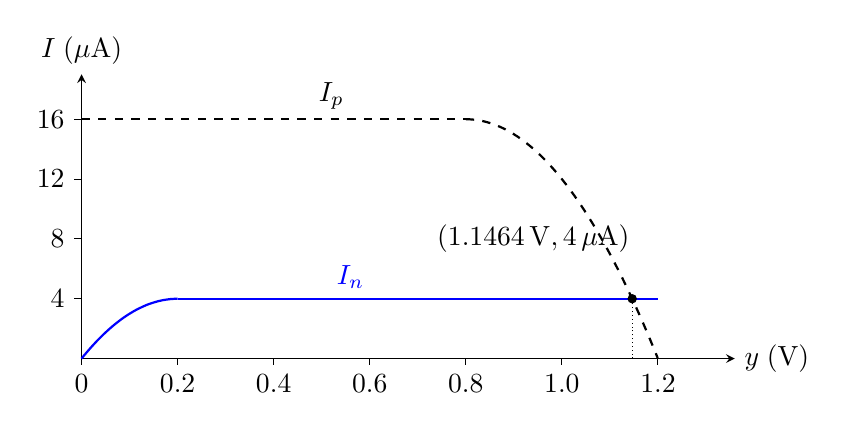
\begin{tikzpicture}[x=6.1cm,y=0.19cm,>=stealth]
\draw[->] (0,0)--(1.36,0) node[right] {\(y\;(\mathrm{V})\)};
\draw[->] (0,0)--(0,19) node[above] {\(I\;(\mu\mathrm{A})\)};
\foreach \x in {0,0.2,0.4,0.6,0.8,1.0,1.2}
 {\draw (\x,0)--(\x,-0.4) node[below] {\(\x\)};}
\foreach \y in {4,8,12,16}
 {\draw (0,\y)--(-0.015,\y) node[left] {\(\y\)};}
\draw[thick,blue,domain=0:0.2,samples=40]
 plot (\x,{200*(0.2*\x-\x*\x/2)});
\draw[thick,blue] (0.2,4)--(1.2,4);
\draw[thick,dashed] (0,16)--(0.8,16);
\draw[thick,dashed,domain=0.8:1.2,samples=45]
 plot (\x,{200*(0.4*(1.2-\x)-(1.2-\x)^2/2)});
\draw[densely dotted] (1.146410,0)--(1.146410,4);
\fill (1.146410,4) circle[radius=1.7pt];
\node[blue,above] at (0.56,4) {\(I_n\)};
\node[above] at (0.52,16) {\(I_p\)};
\node[anchor=west] at (0.72,8) {\((1.1464\,\mathrm{V},4\,\mu\mathrm{A})\)};
\end{tikzpicture}
\end{latin}
\caption{تقاطع جریان‌ها برای یک ورودی فرضی در مدل مربعی متقارن.
ساخت نمودار بر اساس روش شکل \secnum{۲.۲۶} کتاب است.}
\label{fig:inverter-current-intersection}
\end{figure}

جهت تغییر خروجی را نیز می‌توان از همین شکل فهمید. اگر در این
مثال \(y\) از مقدار تعادل کمتر شود، \(I_p>I_n\) و ظرفیت خروجی
شارژ می‌شود. اگر خروجی از تعادل بالاتر برود، \(I_n>I_p\) و خروجی
تخلیه می‌شود. این استدلال، بازگشت خروجی به تعادل را در همسایگی
نقطه نشان می‌دهد. در حالت استثنایی که دو منحنی در بازه‌ای کاملاً
روی هم قرار گیرند، مدل ایده‌آل خروجی یکتا نمی‌دهد. ناحیه \lr{C}
همین حالت را دارد.

\subsubsection{استخراج تحلیلی پنج ناحیه}
\label{sec:inverter-five-regions}
در ادامه فرض‌های \eqref{eq:inverter-symmetry} برقرارند، پس
\(a=V_{\mathrm{in}}-V_t\) و
\(b=V_{DD}-V_{\mathrm{in}}-V_t\) هستند. ترتیب نام‌های
\lr{A} تا \lr{E} از جدول \secnum{۲.۳} کتاب و اسلاید ۷ گرفته
شده است \cite{weste,dcslides}. نام ناحیه مدار، ترکیب ناحیه کاری
دو افزاره را مشخص می‌کند.

\paragraph*{ناحیه \lr{A} و خروجی بالا}
برای \(0\le V_{\mathrm{in}}\le V_t\)، ترانزیستور \lr{nMOS}
در مدل ایده‌آل جریان صفر دارد. چون \(V_{DD}>2V_t\)، ترانزیستور
\lr{pMOS} روشن است. شرط \lr{KCL}، جریان آن را نیز صفر می‌کند.
در شاخه \lr{Linear}، معادله جریان آن چنین است
\[
 0=\beta(bu-u^2/2)=\beta u(b-u/2).
\]
دو جواب جبری \(u=0\) و \(u=2b\) به دست می‌آیند. شرط
\(0\le u<b\) فقط \(u=0\) را می‌پذیرد. بنابراین،
\begin{equation}
 \boxed{V_{\mathrm{out}}=V_{DD},\qquad I_{DD}=0}.
 \label{eq:inverter-region-a}
\end{equation}
ترانزیستور روشن می‌تواند در حالت ماندگار جریان صفر داشته باشد.
اینجا اختلاف ولتاژ سورس و درین \lr{pMOS} صفر شده است. مسیر
هدایت آن، هنگام جابه‌جایی خروجی، بار لازم را فراهم کرده است.

\paragraph*{ناحیه \lr{B} و کاهش اولیه خروجی}
برای \(V_t<V_{\mathrm{in}}<V_{DD}/2\)، ابتدا فرض می‌کنیم
\lr{nMOS} در اشباع و \lr{pMOS} در \lr{Linear} است.
در این بازه \(0<a<b\) داریم. برابری جریان‌ها می‌دهد
\begin{align}
 \frac{\beta a^2}{2}&=\beta(bu-u^2/2),\notag\\
 a^2&=2bu-u^2,\notag\\
 u^2-2bu+a^2&=0,\notag\\
 (u-b)^2&=b^2-a^2.
 \label{eq:inverter-b-quadratic}
\end{align}
در مرحله دوم، تقسیم بر \(\beta>0\) و ضرب در دو انجام شده است.
تمام جمله‌های سه سطر آخر واحد \(\unit{\volt\squared}\) دارند.
با ریشه‌گرفتن، دو پاسخ جبری حاصل می‌شوند.
\[
 u=b\pm\sqrt{b^2-a^2}.
\]
ریشه با علامت مثبت از \(b\) بزرگ‌تر است و شرط \lr{Linear}
برای \lr{pMOS} را نقض می‌کند. ریشه مجاز و خروجی متناظر عبارت‌اند از
\begin{align}
 u&=b-\sqrt{b^2-a^2},\notag\\
 \boxed{V_{\mathrm{out}}=V_{DD}-b+\sqrt{b^2-a^2}}.
 \label{eq:inverter-b-root}
\end{align}
چون \(0<a<b\)، مقدار رادیکال بین صفر و \(b\) است.
پس \(0<u<b\) و \lr{pMOS} واقعاً در \lr{Linear} است.
همچنین \(V_{DD}-b=V_{\mathrm{in}}+V_t\)، پس
ترتیب ولتاژها چنین است.
\[
 V_{\mathrm{out}}>V_{\mathrm{in}}+V_t>V_{\mathrm{in}}-V_t=a.
\]
شرط اشباع \lr{nMOS} نیز برقرار است.
خروجی از تغذیه کمتر است، زیرا \(u>0\).

برای نوشتن خروجی فقط برحسب ورودی، اتحاد تفاضل دو مربع را به کار
می‌بریم. چون \(b-a=V_{DD}-2V_{\mathrm{in}}\) و
\(b+a=V_{DD}-2V_t\)، داریم
\begin{equation}
 \boxed{V_{\mathrm{out}}=V_{\mathrm{in}}+V_t+
 \sqrt{(V_{DD}-2V_{\mathrm{in}})(V_{DD}-2V_t)}}.
 \label{eq:inverter-b-transfer}
\end{equation}
هر دو عامل زیر رادیکال در این بازه مثبت‌اند. ریشه حاصل واحد ولت
دارد. تفاضل دو عدد نزدیک ممکن است در محاسبه عددی، دقت را کم کند.
برای بازنویسی پایدارتر افت ولتاژ نزدیک خروجی بالا، صورت و مخرج را
در مزدوج ضرب می‌کنیم
\[
 b-\sqrt{b^2-a^2}
 =\frac{(b-\sqrt{b^2-a^2})(b+\sqrt{b^2-a^2})}
        {b+\sqrt{b^2-a^2}}
 =\frac{a^2}{b+\sqrt{b^2-a^2}}.
\]
در مرحله آخر، اتحاد تفاضل دو مربع، صورت را به
\(b^2-(b^2-a^2)=a^2\) تبدیل کرده است. بنابراین، برای محاسبه داریم
\begin{equation}
 u=\frac{a^2}{b+\sqrt{b^2-a^2}},\qquad
 V_{\mathrm{out}}=V_{DD}-u.
 \label{eq:inverter-b-stable}
\end{equation}
مخرج مثبت است. با نزدیک‌شدن ورودی به \(V_t\) از بالا،
\(a\to0\)، \(u\to0\) و خروجی به \(V_{DD}\) می‌رسد.
با نزدیک‌شدن ورودی به \(V_{DD}/2\) از پایین،
خروجی به \(V_{DD}/2+V_t\) می‌رسد.

\paragraph*{ناحیه \lr{C} و اشباع هم‌زمان}
وقتی هر دو افزاره در اشباع‌اند، شرط جریان می‌شود
\begin{equation}
 \frac{\beta}{2}(V_{\mathrm{in}}-V_t)^2
 =\frac{\beta}{2}(V_{DD}-V_{\mathrm{in}}-V_t)^2.
 \label{eq:inverter-c-current-equality}
\end{equation}
اضافه‌ولتاژهای دو طرف مثبت‌اند، پس برابرشدن مربع‌ها در این دامنه
به برابری خود اضافه‌ولتاژها می‌انجامد. بنابراین،
\(V_{\mathrm{in}}-V_t=V_{DD}-V_{\mathrm{in}}-V_t\) و در نتیجه
\begin{equation}
 \boxed{V_{\mathrm{in}}=\frac{V_{DD}}{2}}.
 \label{eq:inverter-c-input}
\end{equation}
شرط اشباع \lr{nMOS}، \(V_{\mathrm{out}}\ge V_{DD}/2-V_t\) و
شرط اشباع \lr{pMOS}، \(V_{\mathrm{out}}\le V_{DD}/2+V_t\) است.
پس تمام خروجی‌های بازه زیر معادله ماندگار مدل را برآورده می‌کنند
\begin{equation}
 \boxed{\frac{V_{DD}}{2}-V_t\le V_{\mathrm{out}}
              \le\frac{V_{DD}}{2}+V_t},\qquad
 I_{DD}=\frac{\beta}{2}\left(\frac{V_{DD}}{2}-V_t\right)^2.
 \label{eq:inverter-c-output-interval}
\end{equation}
جریان ایده‌آل اشباع به خروجی وابسته نیست، پس معادله جریان در این
بازه ابزار تعیین خروجی یکتا ندارد. مقدار بار اولیه یا اثرهای
کنارگذاشته‌شده می‌توانند در تعیین خروجی نقش داشته باشند.
روی نمودار، این مجموعه یک پاره‌خط عمودی در
\(V_{\mathrm{in}}=V_{DD}/2\) است. توصیف شیب منفی بی‌نهایت در
کتاب، حد گذار بسیار تند را بیان می‌کند
\cite[صفحه ۸۸]{weste}. در خود مدل ایده‌آل، شیب تابع تک‌مقداری
در این پاره‌خط تعریف نمی‌شود.

\paragraph*{ناحیه \lr{D} و نزدیک‌شدن خروجی به زمین}
برای \(V_{DD}/2<V_{\mathrm{in}}<V_{DD}-V_t\)، فرض می‌کنیم
\lr{nMOS} در \lr{Linear} و \lr{pMOS} در اشباع است.
اینجا \(0<b<a\) داریم و شرط جریان چنین می‌شود
\begin{align}
 \beta(ay-y^2/2)&=\frac{\beta b^2}{2},\notag\\
 y^2-2ay+b^2&=0,\notag\\
 (y-a)^2&=a^2-b^2,\notag\\
 y&=a\pm\sqrt{a^2-b^2}.
 \label{eq:inverter-d-quadratic}
\end{align}
ریشه مثبت از \(a\) بزرگ‌تر است و شرط \lr{Linear} افزاره پایین
را نقض می‌کند. ریشه مجاز برابر است با
\begin{equation}
 \boxed{V_{\mathrm{out}}=a-\sqrt{a^2-b^2}}
 =\frac{b^2}{a+\sqrt{a^2-b^2}}.
 \label{eq:inverter-d-root}
\end{equation}
چون \(0<b<a\)، داریم \(0<y<a\) و شرط \lr{Linear} برقرار است.
همچنین \(y<a=V_{\mathrm{in}}-V_t<
V_{\mathrm{in}}+V_t\)، پس شرط اشباع \lr{pMOS} نیز برقرار است.
با جای‌گذاری \(a-b=2V_{\mathrm{in}}-V_{DD}\) و
\(a+b=V_{DD}-2V_t\)، خروجی برحسب ورودی نوشته می‌شود
\begin{equation}
 \boxed{V_{\mathrm{out}}=V_{\mathrm{in}}-V_t-
 \sqrt{(2V_{\mathrm{in}}-V_{DD})(V_{DD}-2V_t)}}.
 \label{eq:inverter-d-transfer}
\end{equation}
با نزدیک‌شدن ورودی به نقطه میانی از بالا، خروجی به
\(V_{DD}/2-V_t\) می‌رسد. در حد
\(V_{\mathrm{in}}\to V_{DD}-V_t\) از پایین،
\(b\to0\) و خروجی به صفر می‌رسد.

\paragraph*{ناحیه \lr{E} و خروجی پایین}
برای \(V_{DD}-V_t\le V_{\mathrm{in}}\le V_{DD}\)،
\lr{pMOS} در مدل ایده‌آل خاموش و \lr{nMOS} روشن است.
از \lr{KCL}، جریان \lr{nMOS} هم صفر می‌شود.
معادله \(0=\beta y(a-y/2)\) ریشه‌های \(y=0\) و \(y=2a\)
را می‌دهد. شرط \(0\le y<a\)، ریشه صفر را می‌پذیرد. پس
\begin{equation}
 \boxed{V_{\mathrm{out}}=0,\qquad I_{DD}=0}.
 \label{eq:inverter-region-e}
\end{equation}
در این حالت، \lr{nMOS} روشن و اختلاف ولتاژ درین و سورس آن صفر
است. با تغییر کوچک خروجی از زمین، مسیر پایین‌کش می‌تواند بار را
تخلیه کند.

\subsubsection{مشخصه انتقال، جریان تغذیه و مثال عددی}
\label{sec:inverter-transfer-example}
جدول \ref{tab:inverter-five-regions} نتیجه استخراج را با ترتیب
مرجع جمع می‌کند. در مرز بین دو شاخه، می‌توان از هر رابطه‌ای که
شرط مرزی را پوشش می‌دهد استفاده کرد، زیرا جریان‌ها پیوسته‌اند.
در مدل ایده‌آل، مجموعه خروجی‌های \lr{C} بازه مشخصی دارد.
\begin{table}[!htbp]
\centering
\small
\caption{پنج ناحیه مدار برای آستانه‌ها و \(\beta\)های برابر.
فرض \(V_{DD}>2V_t\) برقرار است.}
\label{tab:inverter-five-regions}
\begin{tabular}{cccl}
\toprule
ناحیه & \lr{nMOS} & \lr{pMOS} & شرط ورودی\\
\midrule
\lr{A} & \lr{Cutoff} & \lr{Linear} & \(0\le V_{\mathrm{in}}\le V_t\)\\
\lr{B} & \lr{Saturation} & \lr{Linear} & \(V_t<V_{\mathrm{in}}<V_{DD}/2\)\\
\lr{C} & \lr{Saturation} & \lr{Saturation} & \(V_{\mathrm{in}}=V_{DD}/2\)\\
\lr{D} & \lr{Linear} & \lr{Saturation} & \(V_{DD}/2<V_{\mathrm{in}}<V_{DD}-V_t\)\\
\lr{E} & \lr{Linear} & \lr{Cutoff} & \(V_{DD}-V_t\le V_{\mathrm{in}}\le V_{DD}\)\\
\bottomrule
\end{tabular}
\end{table}

شکل \ref{fig:inverter-ideal-vtc} مشخصه مدل را با نسبت فرضی
\(\tau=V_t/V_{DD}=0.25\) رسم می‌کند. محورهای نرمال‌شده
\(x=V_{\mathrm{in}}/V_{DD}\) و \(z=V_{\mathrm{out}}/V_{DD}\)
بی‌بعدند. از روابط \eqref{eq:inverter-b-transfer} و
\eqref{eq:inverter-d-transfer}، دو شاخه میانی چنین می‌شوند
\begin{equation}
 z_B=x+\tau+\sqrt{(1-2x)(1-2\tau)},\qquad
 z_D=x-\tau-\sqrt{(2x-1)(1-2\tau)}.
 \label{eq:inverter-normalized-vtc}
\end{equation}
در این نمودار، گذار عمودی از \(z=0.75\) تا \(z=0.25\) است.
خروجی در دو سوی این گذار با شاخه‌های رادیکالی تغییر می‌کند.
\begin{figure}[!htbp]
\centering
\begin{latin}
\PersianMathDigits
\begin{tikzpicture}[x=7.3cm,y=4.6cm,>=stealth]
\draw[->] (0,0)--(1.12,0) node[right] {\(V_{\mathrm{in}}/V_{DD}\)};
\draw[->] (0,0)--(0,1.13) node[above] {\(V_{\mathrm{out}}/V_{DD}\)};
\foreach \x in {0.25,0.5,0.75,1.0}
 {\draw (\x,0)--(\x,-0.02) node[below] {\(\x\)};}
\foreach \y in {0.25,0.5,0.75,1.0}
 {\draw (0,\y)--(-0.013,\y) node[left] {\(\y\)};}
\draw[densely dotted] (0,0)--(1,1);
\draw[densely dotted] (0.25,0)--(0.25,1);
\draw[densely dotted] (0.75,0)--(0.75,0.2);
\draw[thick,blue] (0,1)--(0.25,1);
\draw[thick,blue,domain=0.25:0.5,samples=90]
 plot (\x,{\x+0.25+sqrt(max(0,(1-2*\x)*0.5))});
\draw[thick,blue] (0.5,0.75)--(0.5,0.25);
\draw[thick,blue,domain=0.5:0.75,samples=90]
 plot (\x,{\x-0.25-sqrt(max(0,(2*\x-1)*0.5))});
\draw[thick,blue] (0.75,0)--(1,0);
\fill (0.5,0.5) circle[radius=1.6pt];
\node at (0.12,0.9) {A};
\node at (0.36,0.85) {B};
\node[right] at (0.51,0.62) {C};
\node at (0.64,0.15) {D};
\node at (0.9,0.1) {E};
\node[anchor=west] at (0.64,0.57) {\(V_{\mathrm{inv}}/V_{DD}=0.5\)};
\end{tikzpicture}
\end{latin}
\caption{مشخصه انتقال محاسبه‌شده برای مدل متقارن و
\(V_t/V_{DD}=0.25\). خط نقطه‌چین مورب، شرط
\(V_{\mathrm{out}}=V_{\mathrm{in}}\) را نمایش می‌دهد.}
\label{fig:inverter-ideal-vtc}
\end{figure}

در بازه روشن‌بودن هر دو افزاره، جریان مدار از افزاره اشباع‌شده
به دست می‌آید. با تعریف \(A_0=V_{DD}/2-V_t>0\)، نتیجه چنین است
\begin{equation}
 I_{DD}=
 \begin{cases}
 0,&0\le V_{\mathrm{in}}\le V_t,\\[2pt]
 \dfrac{\beta}{2}(V_{\mathrm{in}}-V_t)^2,
     &V_t<V_{\mathrm{in}}\le V_{DD}/2,\\[4pt]
 \dfrac{\beta}{2}(V_{DD}-V_{\mathrm{in}}-V_t)^2,
     &V_{DD}/2<V_{\mathrm{in}}<V_{DD}-V_t,\\[4pt]
 0,&V_{DD}-V_t\le V_{\mathrm{in}}\le V_{DD}.
 \end{cases}
 \label{eq:inverter-supply-current}
\end{equation}
بیشینه جریان این مدل در ورودی میانی برابر
\(I_{DD,\max}=\beta A_0^2/2\) است. شکل
\ref{fig:inverter-supply-current} جریان نرمال‌شده را رسم می‌کند.
\begin{figure}[!htbp]
\centering
\begin{latin}
\PersianMathDigits
\begin{tikzpicture}[x=7.3cm,y=3.3cm,>=stealth]
\draw[->] (0,0)--(1.12,0) node[right] {\(V_{\mathrm{in}}/V_{DD}\)};
\draw[->] (0,0)--(0,1.18) node[above] {\(I_{DD}/I_{DD,\max}\)};
\foreach \x in {0.25,0.5,0.75,1.0}
 {\draw (\x,0)--(\x,-0.025) node[below] {\(\x\)};}
\draw (0,1)--(-0.013,1) node[left] {\(1\)};
\draw[thick,blue] (0,0)--(0.25,0);
\draw[thick,blue,domain=0.25:0.5,samples=45] plot (\x,{16*(\x-0.25)^2});
\draw[thick,blue,domain=0.5:0.75,samples=45] plot (\x,{16*(0.75-\x)^2});
\draw[thick,blue] (0.75,0)--(1,0);
\draw[densely dotted] (0.5,0)--(0.5,1)--(0,1);
\end{tikzpicture}
\end{latin}
\caption{جریان تغذیه مدل مربعی برای نسبت آستانه
\(V_t/V_{DD}=0.25\)، مطابق رابطه \eqref{eq:inverter-supply-current}.
محورها بی‌بعدند.}
\label{fig:inverter-supply-current}
\end{figure}

اگر ورودی در یک مقدار میانی ثابت نگه داشته شود، این جریان در
مدل \lr{DC} به‌طور پیوسته وجود دارد. اگر ورودی از زمین به تغذیه
گذار کند، برای مدتی از بازه هدایت هم‌زمان عبور می‌کند. کتاب این
عبور را با یک پالس جریان توضیح می‌دهد
\cite[شکل \secnum{۲.۲۶} و صفحه ۸۸]{weste}.
شکل جریان برحسب ورودی، زمان و پهنای پالس را تعیین نمی‌کند.
محاسبه جریان طی گذار، به سرعت تغییر ورودی و دینامیک خروجی نیاز دارد.
در ورودی‌های نزدیک دو ریل، جریان ایده‌آل صفر می‌شود. در افزاره
واقعی، نشتی‌های آموزش‌داده‌شده در جزوه دوم وجود دارند.

\paragraph*{محاسبه کامل یک نقطه در \lr{B}}
پارامترهای فرضی شکل \ref{fig:inverter-current-intersection} را
به کار ببرید. در \(V_{\mathrm{in}}=\qty{0.5}{\volt}\)،
\(a=\qty{0.2}{\volt}\) و \(b=\qty{0.4}{\volt}\) است.
از \eqref{eq:inverter-b-root}، افت ولتاژ \lr{pMOS} برابر است با
\begin{equation}
 u=0.4-\sqrt{0.4^2-0.2^2}
   =0.4-\sqrt{0.12}\approx\qty{0.05359}{\volt},\qquad
 y\approx\qty{1.14641}{\volt}.
 \label{eq:inverter-b-numerical}
\end{equation}
ریشه دیگر، \(u\approx\qty{0.74641}{\volt}\)، شرط
\(u<b=\qty{0.4}{\volt}\) را نقض می‌کند. برای ریشه مجاز،
\(y>\qty{0.2}{\volt}\) و \(u<\qty{0.4}{\volt}\) هستند.
پس \lr{nMOS} در اشباع و \lr{pMOS} در \lr{Linear} است.
محاسبه دو جریان به‌صورت مستقل می‌دهد
\begin{align}
 I_n&=(200/2)(0.2)^2=\qty{4.000}{\micro\ampere},\notag\\
 I_p&=200[0.4(0.0535898)-(0.0535898)^2/2]
       \approx\qty{4.000}{\micro\ampere}.
 \label{eq:inverter-b-current-check}
\end{align}
در سطرهای عددی، ضریب جریان برحسب
\(\unit{\micro\ampere\per\volt\squared}\) و ولتاژها برحسب ولت
جای‌گذاری شده‌اند. توان دریافت‌شده از تغذیه در این نقطه چنین است.
\[
 P=V_{DD}I_{DD}=1.2(4)=\qty{4.8}{\micro\watt}.
\]

\paragraph*{محاسبه کامل یک نقطه در \lr{D}}
در همان مدار، اگر \(V_{\mathrm{in}}=\qty{0.7}{\volt}\)،
\(a=\qty{0.4}{\volt}\) و \(b=\qty{0.2}{\volt}\) می‌شود.
از \eqref{eq:inverter-d-root}، خروجی به دست می‌آید.
\[
 y=0.4-\sqrt{0.4^2-0.2^2}\approx\qty{0.05359}{\volt}.
\]
ریشه بزرگ‌تر \(y\approx\qty{0.74641}{\volt}\) از
\(a=\qty{0.4}{\volt}\) بیشتر است و شرط \lr{Linear}
برای \lr{nMOS} را نقض می‌کند. برای ریشه مجاز،
\(y<a\) و \(u=1.2-y\approx\qty{1.14641}{\volt}>b\) هستند.
پس \lr{nMOS} در \lr{Linear} و \lr{pMOS} در اشباع است.
دو جریان برابر \(\qty{4}{\micro\ampere}\) و توان نیز
\(\qty{4.8}{\micro\watt}\) است.

جدول \ref{tab:inverter-numerical-transfer} چند نقطه دیگر را نشان
می‌دهد. به‌دلیل تقارن، خروجی‌ها در دو ورودی مکمل به‌صورت
\(y(V_{DD}-v)=V_{DD}-y(v)\) مرتبط‌اند. در ورودی میانی،
\(y\in[\qty{0.3}{\volt},\qty{0.9}{\volt}]\) و جریان
\(\qty{9}{\micro\ampere}\) است. توان ماندگار آن نقطه در مدل
ایده‌آل \(\qty{10.8}{\micro\watt}\) می‌شود.
\begin{table}[!htbp]
\centering
\small
\caption{نمونه‌های محاسبه‌شده برای پارامترهای فرضی
\(V_{DD}=\qty{1.2}{\volt}\)، \(V_t=\qty{0.3}{\volt}\) و
\(\beta=\qty{200}{\micro\ampere\per\volt\squared}\).
اعداد تا رقم‌های نمایش‌داده‌شده گرد شده‌اند.}
\label{tab:inverter-numerical-transfer}
\begin{tabular}{cccc}
\toprule
\(V_{\mathrm{in}}\)، \(\unit{\volt}\) &
\(V_{\mathrm{out}}\)، \(\unit{\volt}\) &
\(I_{DD}\)، \(\unit{\micro\ampere}\) & ناحیه\\
\midrule
\num{0.00} & \num{1.2000} & \num{0} & \lr{A}\\
\num{0.30} & \num{1.2000} & \num{0} & مرز \lr{A/B}\\
\num{0.40} & \num{1.1899} & \num{1.00} & \lr{B}\\
\num{0.50} & \num{1.1464} & \num{4.00} & \lr{B}\\
\num{0.55} & \num{1.0949} & \num{6.25} & \lr{B}\\
\num{0.60} & بازه \(0.3\le y\le0.9\) & \num{9.00} & \lr{C}\\
\num{0.65} & \num{0.1051} & \num{6.25} & \lr{D}\\
\num{0.70} & \num{0.0536} & \num{4.00} & \lr{D}\\
\num{0.80} & \num{0.0101} & \num{1.00} & \lr{D}\\
\num{0.90} & \num{0.0000} & \num{0} & مرز \lr{D/E}\\
\num{1.20} & \num{0.0000} & \num{0} & \lr{E}\\
\bottomrule
\end{tabular}
\end{table}

\subsubsection{شیب مشخصه و اثر \lr{CLM}}
\label{sec:inverter-clm}
در مدل ایده‌آل، \(I_n\) و \(I_p\) در اشباع به ولتاژ خروجی
وابسته نیستند. \lr{CLM} این استقلال را تغییر می‌دهد و مقاومت
خروجی محدود ایجاد می‌کند. کتاب، همین اثر را علت شیب محدود و
گسترش ناحیه \lr{C} واقعی به بازه‌ای از ورودی‌ها می‌داند
\cite[صفحه ۸۸ و بخش \secnum{۲.۴.۲}]{weste}.

برای نمایش تحلیلی این نکته، تنها در دامنه اشباع هم‌زمان، مدل
مربعی با \lr{CLM} را به کار می‌بریم. تعریف کنید
\(N=\beta_na^2/2\) و \(P=\beta_pb^2/2\). این دو کمیت واحد
آمپر دارند. آنگاه با \(\lambda_n,\lambda_p>0\) داریم
\begin{equation}
 I_n=N(1+\lambda_n y),\qquad
 I_p=P[1+\lambda_p(V_{DD}-y)].
 \label{eq:inverter-clm-currents}
\end{equation}
عامل‌های داخل پرانتز بی‌بعدند و واحد \(\lambda\)،
\(\unit{\per\volt}\) است. برابری جریان‌ها به‌صورت خطی برحسب
خروجی حل می‌شود
\begin{align}
 N+N\lambda_n y&=P+P\lambda_pV_{DD}-P\lambda_p y,\notag\\
 (N\lambda_n+P\lambda_p)y&=P(1+\lambda_pV_{DD})-N,\notag\\
 \boxed{y=\frac{P(1+\lambda_pV_{DD})-N}
                    {N\lambda_n+P\lambda_p}}.
 \label{eq:inverter-clm-output}
\end{align}
صورت واحد آمپر و مخرج واحد آمپر بر ولت دارد، پس جواب ولتاژ است.
پس از حل باید \(a,b>0\) و
\(a\le y\le V_{\mathrm{in}}+V_{TP}\) بررسی شوند. این رابطه
فقط در محدوده‌ای که هر دو افزاره در اشباع‌اند معتبر است.
اگر یکی از شرط‌ها نقض شود، رابطه جریان همان افزاره باید عوض شود.

\paragraph*{مثال آموزشی خروجی یکتا در ناحیه میانی}
به پارامترهای فرضی قبلی،
\(\lambda_n=\lambda_p=\qty{0.1}{\per\volt}\) اضافه کنید.
در \(V_{\mathrm{in}}=\qty{0.6}{\volt}\)، داریم
\(a=b=\qty{0.3}{\volt}\) و \(N=P=\qty{9}{\micro\ampere}\).
رابطه \eqref{eq:inverter-clm-output} می‌دهد
\[
 y=\frac{9(1+0.1\times1.2)-9}{9(0.1)+9(0.1)}
 =\qty{0.6}{\volt}.
\]
هر دو شرط اشباع برقرارند، زیرا
\(\qty{0.3}{\volt}\le y\le\qty{0.9}{\volt}\).
جریان از رابطه مدل به دست می‌آید.
\[
 I_{DD}=9(1+0.1\times0.6)=\qty{9.54}{\micro\ampere}.
\]
جدول \ref{tab:inverter-clm-results} چند ورودی نزدیک را
نشان می‌دهد. همه ردیف‌های جدول، پس از کنترل ناحیه کاری پذیرفته
شده‌اند. اعداد، نتیجه مدل آموزشی‌اند.
\begin{table}[!htbp]
\centering
\caption{اثر \lr{CLM} در چند نقطه با اشباع هم‌زمان، برای
\(\lambda_n=\lambda_p=\qty{0.1}{\per\volt}\) و پارامترهای مثال.}
\label{tab:inverter-clm-results}
\begin{tabular}{ccc}
\toprule
\(V_{\mathrm{in}}\)، \(\unit{\volt}\) &
\(V_{\mathrm{out}}\)، \(\unit{\volt}\) &
\(I_{DD}\)، \(\unit{\micro\ampere}\)\\
\midrule
\num{0.596} & \num{0.8826} & \num{9.5349}\\
\num{0.598} & \num{0.7413} & \num{9.5387}\\
\num{0.600} & \num{0.6000} & \num{9.5400}\\
\num{0.602} & \num{0.4587} & \num{9.5387}\\
\num{0.604} & \num{0.3174} & \num{9.5349}\\
\bottomrule
\end{tabular}
\end{table}

برای نمونه، به‌کاربردن همین رابطه در
\(V_{\mathrm{in}}=\qty{0.595}{\volt}\)، خروجی
\(y\approx\qty{0.9532}{\volt}\) می‌دهد. اما حد اشباع
\lr{pMOS} در آن ورودی \(y\le\qty{0.895}{\volt}\) است.
پس این پاسخ با فرض اشباع هم‌زمان سازگار نیست و باید با ترکیب
\lr{Saturation/Linear} دوباره حل شود. قرارگرفتن عدد در بازه
زمین تا تغذیه به‌تنهایی برای پذیرش جواب کافی نیست.

\paragraph*{استخراج \lr{Gain} با تغییرهای کوچک}
برای یک تغییر کوچک ورودی و خروجی در نقطه اشباع هم‌زمان،
جریان \lr{nMOS} را به‌صورت زیر تغییر می‌دهیم
\begin{equation}
 \mathrm{d}I_n=g_{m,n}\,\mathrm{d}V_{\mathrm{in}}
                +g_{ds,n}\,\mathrm{d}y.
 \label{eq:inverter-small-change-n}
\end{equation}
در اینجا \(g_{m,n}>0\) نرخ تغییر جریان با گیت در خروجی ثابت و
\(g_{ds,n}>0\) نرخ تغییر آن با خروجی در ورودی ثابت است.
هر دو واحد \(\unit{\siemens}=\unit{\ampere\per\volt}\) دارند.
برای بزرگی جریان \lr{pMOS}، افزایش ورودی، \(V_{SG,p}\) را کم
می‌کند و افزایش خروجی، \(V_{SD,p}\) را کم می‌کند. بنابراین،
\begin{equation}
 \mathrm{d}I_p=-g_{m,p}\,\mathrm{d}V_{\mathrm{in}}
                 -g_{ds,p}\,\mathrm{d}y.
 \label{eq:inverter-small-change-p}
\end{equation}
کمیت‌های \(g_{m,p},g_{ds,p}\) نیز بزرگی‌های مثبت‌اند. با
قرارگرفتن هر دو حالت نزدیک در تعادل، باید
\(\mathrm{d}I_n=\mathrm{d}I_p\) باشد. با جمع جمله‌ها نتیجه می‌شود
\begin{equation}
 \boxed{\frac{\mathrm{d}V_{\mathrm{out}}}{\mathrm{d}V_{\mathrm{in}}}
 =-\frac{g_{m,n}+g_{m,p}}{g_{ds,n}+g_{ds,p}}}.
 \label{eq:inverter-gain}
\end{equation}
این استخراج تکمیلی، اثر مقاومت خروجی محدود بر شیب را روشن می‌کند.
در مدل \eqref{eq:inverter-clm-currents}، مشتق‌ها چنین‌اند
\begin{align}
 g_{m,n}&=\beta_na(1+\lambda_n y),&
 g_{ds,n}&=\lambda_nN,\notag\\
 g_{m,p}&=\beta_pb[1+\lambda_p(V_{DD}-y)],&
 g_{ds,p}&=\lambda_pP.
 \label{eq:inverter-clm-derivatives}
\end{align}
در مرکز مثال، رسانایی‌ها چنین‌اند.
\[
 \begin{aligned}
 g_{m,n}=g_{m,p}&=\qty{63.6}{\micro\siemens},\\
 g_{ds,n}=g_{ds,p}&=\qty{0.9}{\micro\siemens}.
 \end{aligned}
\]
پس شیب محلی از نسبت رسانایی‌ها به دست می‌آید.
\[
 -\frac{63.6+63.6}{0.9+0.9}\approx-70.67.
\]
تغییر ورودی \(\qty{1}{\milli\volt}\) در همسایگی مرکز، حدود
\(\qty{70.7}{\milli\volt}\) تغییر خروجی در جهت مخالف ایجاد
می‌کند. این برآورد، تقریب خطی محلی است.

با میل \(\lambda_n,\lambda_p\) به صفر، رسانایی خروجی مدل به
صفر می‌رود و بزرگی شیب افزایش می‌یابد. در حد کاملاً ایده‌آل،
همان گذار عمودی و بازه خروجی ناحیه \lr{C} بازیابی می‌شود.
کتاب در شکل \secnum{۲.۲۷}، نتیجه شبیه‌سازی یک نمونه فناوری
\(\qty{65}{\nano\metre}\) را نشان می‌دهد که \lr{pMOS} آن دو
برابر \lr{nMOS} عرض دارد. شکل مرجع، گذار تند با شیب محدود را
نمایش می‌دهد \cite[صفحه ۸۹]{weste}. پارامترهای عددی این جزوه
برای توضیح مدل فرض شده‌اند و به آن نمونه نسبت داده نمی‌شوند.

\subsubsection{آستانه ورودی \lr{Inverter} و وابستگی دمایی}
\label{sec:inverter-input-threshold}
کتاب نقطه تقاطع مشخصه انتقال با خط
\(V_{\mathrm{out}}=V_{\mathrm{in}}\) را
\lr{Input Threshold} یا \(V_{\mathrm{inv}}\) می‌نامد
\cite[صفحه ۸۹]{weste}. بنابراین، تعریف این ولتاژ چنین است
\begin{equation}
 V_{\mathrm{out}}=V_{\mathrm{in}}=V_{\mathrm{inv}}.
 \label{eq:inverter-threshold-definition}
\end{equation}
آستانه \(V_t\) پارامتر یک ترانزیستور است. آستانه
\(V_{\mathrm{inv}}\) با برابرشدن ولتاژ ورودی و خروجی کل مدار
تعریف می‌شود. مثلاً در مثال حاضر، \(V_t=\qty{0.3}{\volt}\) و
\(V_{\mathrm{inv}}=\qty{0.6}{\volt}\) هستند.

در مدل متقارن، نقطه \(V_{DD}/2\) هم در بازه خروجی
\eqref{eq:inverter-c-output-interval} قرار دارد و هم شرط
\eqref{eq:inverter-threshold-definition} را برقرار می‌کند. پس
\begin{equation}
 \boxed{V_{\mathrm{inv}}=V_{DD}/2}.
 \label{eq:inverter-symmetric-threshold}
\end{equation}
این تعریف، از میان خروجی‌های مجاز مدل ایده‌آل، محل تقاطع با خط
مورب را مشخص می‌کند. در مدل متقارن با \lr{CLM} یکسان نیز
\(N=P\) در مرکز و رابطه \eqref{eq:inverter-clm-output} همان
خروجی \(V_{DD}/2\) را می‌دهد.

کتاب بیان می‌کند که کاهش \lr{Mobility} و بزرگی آستانه با دما
برای هر دو نوع افزاره رخ می‌دهد و آستانه ورودی مدار معمولاً
حساسیت دمایی کمتری دارد \cite[صفحه ۸۹]{weste}. در فرض تقارن
کامل و تغذیه ثابت، اگر دو آستانه در هر دما برابر و دو
\(\beta\) نیز در هر دما برابر بمانند، رابطه
\eqref{eq:inverter-symmetric-threshold} دقیقاً حفظ می‌شود.
خود جریان‌ها همچنان می‌توانند به‌شدت با دما تغییر کنند.
در مدار واقعی، تفاوت تغییر پارامترهای دو نوع افزاره و تغییر
تغذیه می‌تواند نقطه تقاطع را جابه‌جا کند. نسبت‌های نابرابر
\(\beta\) موضوع بخش \secnum{۲.۵.۲} هستند.

\subsubsection{تمرین‌های تشریحی و کنترل تحلیل}
\label{sec:inverter-practice}
\paragraph*{تمرین آموزشی ۱ و بررسی شرط‌های \lr{pMOS}}
فرض کنید \(V_{DD}=\qty{1.2}{\volt}\)،
\(V_{\mathrm{in}}=\qty{0.5}{\volt}\)،
\(V_{\mathrm{out}}=\qty{1.1}{\volt}\) و
\(V_{tp}=-\qty{0.3}{\volt}\) باشند. ناحیه کاری \lr{pMOS}
را با هر دو قرارداد ولتاژ تعیین کنید.

\textbf{پاسخ.}
در قرارداد مثبت، اختلاف ولتاژها چنین‌اند.
\[
 \begin{aligned}
 V_{SG,p}&=1.2-0.5=\qty{0.7}{\volt},\\
 V_{SD,p}&=1.2-1.1=\qty{0.1}{\volt}.
 \end{aligned}
\]
اضافه‌ولتاژ \(0.7-0.3=\qty{0.4}{\volt}\) و شرط
\(0.1<0.4\) برقرار است، پس افزاره در \lr{Linear} است.
در قرارداد علامت‌دار، \(V_{GS,p}=-\qty{0.7}{\volt}<V_{tp}\)
و \(V_{DS,p}=-\qty{0.1}{\volt}\) هستند.
شرط \(V_{DS,p}>V_{GS,p}-V_{tp}\) یعنی
نامساوی زیر نیز برقرار است.
\[
 -0.1>-0.7-(-0.3)=-0.4.
\]
برای ادعای تعادل کل مدار، باید جریان \lr{nMOS} و \lr{pMOS}
هم بررسی شوند. تعیین ناحیه یک افزاره، تعادل کل مدار را ثابت نمی‌کند.

\paragraph*{تمرین آموزشی ۲ و تشخیص ریشه فیزیکی}
در مدار متقارن مثال، برای ورودی \(\qty{0.7}{\volt}\)،
شخصی خروجی \(\qty{0.7464}{\volt}\) را از معادله درجه دوم
گزارش می‌کند. این جواب را بررسی کنید.

\textbf{پاسخ.}
در فرض ناحیه \lr{D}، باید \lr{nMOS} در \lr{Linear} باشد، یعنی
\(y<V_{\mathrm{in}}-V_t=\qty{0.4}{\volt}\).
ریشه گزارش‌شده این شرط را نقض می‌کند.
ریشه \(\qty{0.05359}{\volt}\) از \eqref{eq:inverter-d-root}
هم شرط \lr{nMOS} و هم شرط اشباع \lr{pMOS} را برآورده می‌کند.
پس باید همین ریشه انتخاب شود. هر دو ریشه معادله جبری را حل
می‌کنند، اما معادله با فرض یک ناحیه خاص استخراج شده است.

\paragraph*{تمرین آموزشی ۳ و مقیاس‌کردن جریان}
در مدل متقارن، هر دو \(\beta\) را دو برابر کنید و آستانه، تغذیه
و فرض بار \lr{DC} را ثابت نگه دارید. مشخصه انتقال و جریان چه
تغییری می‌کنند؟

\textbf{پاسخ.}
در \(I_n=I_p\)، ضریب مشترک دو از دو طرف حذف می‌شود، پس همان
خروجی‌ها به دست می‌آیند. در \(V_{\mathrm{in}}=\qty{0.5}{\volt}\)،
خروجی همچنان \(\qty{1.1464}{\volt}\) است، اما جریان از
\(\qty{4}{\micro\ampere}\) به \(\qty{8}{\micro\ampere}\)
می‌رسد. توان ماندگار این نقطه نیز از
\(\qty{4.8}{\micro\watt}\) به \(\qty{9.6}{\micro\watt}\)
می‌رسد. برای زمان گذار، تغییر ظرفیت ناشی از تغییر ابعاد نیز باید
در مدل دینامیکی وارد شود.

\paragraph*{تمرین آموزشی ۴ و ولتاژ میانی ایده‌آل}
در ورودی \(\qty{0.6}{\volt}\) مثال ایده‌آل، خروجی‌های
\(\qty{0.4}{\volt}\) و \(\qty{0.8}{\volt}\) را آزمایش کنید.
آیا هر دو می‌توانند شرط \lr{DC} مدل را برقرار کنند؟

\textbf{پاسخ.}
در هر دو حالت، اضافه‌ولتاژهای \(a=b=\qty{0.3}{\volt}\)
هستند. خروجی اول، \(y=\qty{0.4}{\volt}\ge a\) و
\(u=\qty{0.8}{\volt}\ge b\) می‌دهد. خروجی دوم،
\(y=\qty{0.8}{\volt}\ge a\) و
\(u=\qty{0.4}{\volt}\ge b\) می‌دهد.
پس هر دو افزاره در هر دو حالت اشباع‌اند و جریان‌ها
\(\qty{9}{\micro\ampere}\) هستند. هر دو خروجی در مدل ایده‌آل
تعادل دارند. با مدل \lr{CLM} متقارن مثال، حل یکتای مرکزی
\(\qty{0.6}{\volt}\) به دست می‌آید.

\paragraph*{مرور روش حل}
ابتدا ولتاژ سورس، گیت، درین و بدنه را بنویسید. قرارداد آستانه
\lr{pMOS} را مشخص کنید. جریان بار و فرض حالت ماندگار را تعیین
کنید. سپس اضافه‌ولتاژها و ترکیب ناحیه کاری را بنویسید، جریان‌ها
را برابر بگذارید و معادله را حل کنید. هر ریشه باید با شرط‌های
ناحیه کاری، بازه زمین تا تغذیه و واحدها کنترل شود. در نقطه میانی
مدل ایده‌آل، بازه خروجی را نگه دارید. برای مدل واقعی‌تر، اثرهای
غیرایده‌آل را با قرارداد یکسان و پارامترهای مشخص وارد کنید.

% !TeX root = booklet-03.tex
\clearpage
\subsection{اثر نسبت \lr{Beta}}
\label{sec:beta-ratio}
در بخش قبل، \(\beta_n=\beta_p\) و بزرگی دو آستانه برابر بود.
اکنون نسبت قدرت دو مسیر را تغییر می‌دهیم و اثر آن بر
\(V_{\mathrm{inv}}\) را استخراج می‌کنیم. مبنای این بخش، روابط
\secnum{۲.۵۴} تا \secnum{۲.۵۷}، شکل \secnum{۲.۲۸} کتاب و
اسلاید ۸ است \cite[بخش \secnum{۲.۵.۲}، صفحات ۹۰ و ابتدای ۹۱]{weste}
\cite[اسلاید ۸]{dcslides}. همه جریان‌ها با قرارداد مثبت
\(I_n=I_{DS,n}\) و \(I_p=|I_{DS,p}|\) بخش
\ref{sec:inverter-conventions} نوشته می‌شوند.

\subsubsection{معنای نسبت و \lr{Skew}}
\label{sec:beta-skew-definition}
نسبت \lr{Beta} در مدل \lr{Long-channel} را چنین تعریف می‌کنیم
\begin{equation}
 \boxed{r_\beta=\frac{\beta_p}{\beta_n}}>0.
 \label{eq:beta-ratio-definition}
\end{equation}
هر دو \(\beta\) واحد \(\unit{\ampere\per\volt\squared}\) دارند،
پس \(r_\beta\) بی‌بعد است. مثلاً اگر
\(\beta_n=\qty{200}{\micro\ampere\per\volt\squared}\) و
\(\beta_p=\qty{800}{\micro\ampere\per\volt\squared}\) باشند،
\(r_\beta=4\) است. در اضافه‌ولتاژ گیت و ناحیه کاری یکسان،
ضریب جریان \lr{pMOS} در این مدل چهار برابر است.

در قرارداد کتاب، \(r_\beta>1\) را \lr{HI-skewed}،
\(r_\beta<1\) را \lr{LO-skewed} و \(r_\beta=1\) را
\lr{Unskewed} می‌نامند \cite[صفحه ۹۰]{weste}.
برای آستانه‌های با بزرگی برابر، \lr{HI-skewed} مسیر بالاکش
قوی‌تری دارد. در ورودی میانی، افزایش جریان بالاکش، بار خروجی
را بیشتر می‌کند و خروجی بالاتر می‌رود. برای برقراری دوباره تعادل
در شرط \(V_{\mathrm{out}}=V_{\mathrm{in}}\)، باید ورودی بالاتر
رود تا جریان \lr{nMOS} بیشتر و جریان \lr{pMOS} کمتر شود.
پس آستانه ورودی به سمت ولتاژ بالاتر جابه‌جا می‌شود.
در \lr{LO-skewed}، جهت جابه‌جایی معکوس است.

برابری \(\beta\) و بزرگی آستانه‌ها، تقارن دو مسیر را در مدل
ساده ایجاد می‌کند. مرجع این تقارن را برای حاشیه‌های منطقی
متوازن و توانایی مشابه شارژ و تخلیه بار خازنی مطلوب می‌داند
\cite[آغاز بخش \secnum{۲.۵.۲}]{weste}.
برابری زمان شارژ و تخلیه به تقارن مدل جریان، بار و شرایط تحریک
نیز وابسته است. تحلیل حاشیه‌های منطقی در بخش \secnum{۲.۵.۳}
تکمیل می‌شود.

\subsubsection{استخراج آستانه در مدل \lr{Long-channel}}
\label{sec:beta-long-channel}
برای جلوگیری از اشتباه علامت، دو ولتاژ مرزی را تعریف می‌کنیم
\begin{equation}
 L=V_{tn},\qquad H=V_{DD}-V_{TP}=V_{DD}+V_{tp},\qquad
 \Delta=H-L>0.
 \label{eq:beta-window}
\end{equation}
نمادهای \(L\) و \(H\) در این بخش ولتاژند. طول کانال در روابط
هندسی با زیرنویس افزاره، مانند \(L_n\)، نوشته می‌شود.
بازه \(L<V_{\mathrm{in}}<H\) بازه روشن‌بودن هم‌زمان دو
افزاره در مدل هدایت قوی است. شرط \(\Delta>0\) یعنی
\(V_{DD}>V_{tn}+V_{TP}\).

آستانه ورودی با \(V_{\mathrm{in}}=V_{\mathrm{out}}=M\) تعریف
می‌شود که در این بخش \(M=V_{\mathrm{inv}}\) است.
در این نقطه، \lr{nMOS} روشن شرط اشباع را خودبه‌خود دارد، زیرا
\(V_{DS,n}=M\ge M-V_{tn}\). برای \lr{pMOS} نیز
\(V_{SD,p}=V_{DD}-M\ge V_{DD}-M-V_{TP}\) برقرار است.
پس اگر \(L<M<H\) باشد، هر دو در اشباع‌اند.
با استفاده از مدل مربعی رابطه \secnum{۲.۵۴} کتاب می‌نویسیم
\begin{equation}
 I_n=\frac{\beta_n}{2}(M-L)^2,\qquad
 I_p=\frac{\beta_p}{2}(H-M)^2.
 \label{eq:beta-long-currents}
\end{equation}
در قرارداد علامت‌دار کتاب، جریان \lr{pMOS} در جهت درین به
سورس منفی است. برابری بزرگی جریان‌ها در قرارداد حاضر، همان
\lr{KCL} گره خروجی را اعمال می‌کند.

تقسیم دو طرف معادله جریان بر \(\beta_n/2>0\) می‌دهد
\begin{align}
 (M-L)^2&=r_\beta(H-M)^2,\notag\\
 M-L&=\sqrt{r_\beta}(H-M).
 \label{eq:beta-positive-root}
\end{align}
در سطر دوم از مثبت‌بودن هر دو اضافه‌ولتاژ استفاده شده است.
اگر صرفاً از برابری مربع‌ها ریشه مثبت و منفی بگیریم، باید شرط
روشن‌بودن هر دو افزاره را هم اعمال کنیم. در بازه مورد نظر،
\(M-L>0\) و \(H-M>0\) هستند و علامت مثبت لازم است.

با تعریف \(s=\sqrt{r_\beta}>0\)، جمله‌های شامل \(M\) را جمع می‌کنیم
\begin{align}
 M-L&=sH-sM,\notag\\
 M+sM&=L+sH,\notag\\
 \boxed{M=\frac{L+sH}{1+s}
 =\frac{V_{tn}+\sqrt{r_\beta}(V_{DD}-V_{TP})}
              {1+\sqrt{r_\beta}}}.
 \label{eq:beta-long-threshold}
\end{align}
صورت واحد ولت و مخرج بی‌بعد دارد. با تقسیم صورت و مخرج بر
\(s\) و جای‌گذاری \(V_{TP}=-V_{tp}\)، شکل نوشته‌شده در
رابطه \secnum{۲.۵۵} کتاب به دست می‌آید
\begin{equation}
 M=\frac{V_{DD}+V_{tp}+V_{tn}\sqrt{1/r_\beta}}
              {1+\sqrt{1/r_\beta}}.
 \label{eq:beta-book-long-form}
\end{equation}
عبارت \(V_{DD}+V_{tp}\)، با منفی‌بودن \(V_{tp}\)، همان
\(V_{DD}-V_{TP}\) است.

\paragraph*{کنترل جواب و رفتار حدی}
برای اثبات قرارگرفتن جواب در دامنه، از
\eqref{eq:beta-long-threshold} دو تفاضل را محاسبه می‌کنیم
\begin{equation}
 M-L=\frac{s\Delta}{1+s}>0,\qquad
 H-M=\frac{\Delta}{1+s}>0.
 \label{eq:beta-threshold-domain}
\end{equation}
پس فرض روشن‌بودن و اشباع هم‌زمان سازگار است. همچنین \(M\)
یک میانگین وزنی از دو ولتاژ مرزی است. افزایش وزن \(H\)، جواب
را به سمت \(H\) می‌برد. برای \(r_\beta\to0^+\)،
\(M\to L\) و برای \(r_\beta\to\infty\)، \(M\to H\).
این دو، حد نسبت‌های مثبت‌اند. اگر یکی از ضریب‌های جریان دقیقاً
صفر باشد، فرض وجود دو مسیر فعال باید دوباره بررسی شود.

در \(r_\beta=1\)، جواب برابر است با
\begin{equation}
 M=\frac{L+H}{2}
   =\frac{V_{DD}+V_{tn}-V_{TP}}{2}.
 \label{eq:beta-equal-strength}
\end{equation}
برای \(V_{tn}=V_{TP}\)، مقدار \(V_{DD}/2\) بازیابی می‌شود.
بنابراین، ادعای آستانه میانی با \(r_\beta=1\)، فرض برابری
بزرگی آستانه‌ها را نیز در خود دارد.

\paragraph*{مثال آموزشی آستانه و کنترل دو جریان}
فرض کنید \(V_{DD}=\qty{1.2}{\volt}\)،
\(V_{tn}=V_{TP}=\qty{0.3}{\volt}\)،
\(\beta_n=\qty{200}{\micro\ampere\per\volt\squared}\) و
\(\beta_p=\qty{800}{\micro\ampere\per\volt\squared}\) باشند.
این پارامترها برای آموزش فرض شده‌اند. داریم
\(L=\qty{0.3}{\volt}\)، \(H=\qty{0.9}{\volt}\)،
\(r_\beta=4\) و \(s=2\). پس
\begin{equation*}
 M=\frac{0.3+2(0.9)}{1+2}=\qty{0.7}{\volt}.
\end{equation*}
اضافه‌ولتاژ \lr{nMOS} برابر \(\qty{0.4}{\volt}\) و
اضافه‌ولتاژ \lr{pMOS} برابر \(\qty{0.2}{\volt}\) است.
در \(V_{\mathrm{out}}=M\)، ولتاژهای درین و سورس متناظر
\(V_{DS,n}=\qty{0.7}{\volt}\) و
\(V_{SD,p}=\qty{0.5}{\volt}\) هستند، پس هر دو شرط اشباع برقرارند.
کنترل مستقل جریان‌ها می‌دهد
\begin{equation*}
 I_n=(200/2)(0.4)^2=\qty{16}{\micro\ampere},\qquad
 I_p=(800/2)(0.2)^2=\qty{16}{\micro\ampere}.
\end{equation*}
قوی‌ترشدن مسیر \lr{pMOS}، آستانه را از
\(\qty{0.6}{\volt}\) در حالت متقارن به
\(\qty{0.7}{\volt}\) رسانده است.

\subsubsection{اثر نسبت بر تمام مشخصه انتقال}
\label{sec:beta-transfer-curves}
در مدل ایده‌آل، تغییر نسبت، محل گذار تند را جابه‌جا می‌کند.
برای نشان‌دادن این اثر، استخراج ناحیه‌های \lr{B} و \lr{D}
بخش \ref{sec:inverter-five-regions} را با دو ضریب متفاوت انجام
می‌دهیم. همچنان \(a=V_{\mathrm{in}}-V_{tn}\)،
\(b=V_{DD}-V_{\mathrm{in}}-V_{TP}\)،
\(u=V_{DD}-y\) و \(y=V_{\mathrm{out}}\) هستند.
در \lr{B}، \lr{nMOS} در اشباع و \lr{pMOS} در \lr{Linear} است.
پس
\begin{align}
 \frac{\beta_n a^2}{2}&=\beta_p(bu-u^2/2),\notag\\
 u^2-2bu+\frac{a^2}{r_\beta}&=0,\notag\\
 \boxed{y=V_{DD}-b+\sqrt{b^2-a^2/r_\beta}}.
 \label{eq:beta-b-transfer}
\end{align}
ریشه انتخاب‌شده همان ریشه‌ای است که \(0\le u\le b\) می‌دهد.
در \(L<V_{\mathrm{in}}<M\)، رابطه
\(a<\sqrt{r_\beta}b\) برقرار است و رادیکال حقیقی می‌ماند.
در \lr{D}، با \lr{nMOS} در \lr{Linear} و \lr{pMOS} در
اشباع، داریم
\begin{align}
 \beta_n(ay-y^2/2)&=\frac{\beta_pb^2}{2},\notag\\
 y^2-2ay+r_\beta b^2&=0,\notag\\
 \boxed{y=a-\sqrt{a^2-r_\beta b^2}}.
 \label{eq:beta-d-transfer}
\end{align}
در \(M<V_{\mathrm{in}}<H\)، رادیکال حقیقی و ریشه مجاز در
\(0\le y\le a\) است. در نقطه گذار \(V_{\mathrm{in}}=M\)،
خروجی‌های اشباع هم‌زمان در بازه زیر قرار دارند
\begin{equation}
 M-V_{tn}\le y\le M+V_{TP}.
 \label{eq:beta-c-interval}
\end{equation}
در ورودی‌های \(V_{\mathrm{in}}\le L\)، خروجی ایده‌آل
\(V_{DD}\) و در \(V_{\mathrm{in}}\ge H\)، خروجی صفر است.
شرط‌های هر شاخه با روش بخش قبل کنترل می‌شوند.

شکل \ref{fig:beta-vtc-family} سه مشخصه فرضی با
\(V_{tn}=V_{TP}=0.25V_{DD}\) را نشان می‌دهد. منحنی‌ها مستقیماً
از \eqref{eq:beta-b-transfer}، \eqref{eq:beta-d-transfer} و
\eqref{eq:beta-c-interval} رسم شده‌اند. این شکل، توضیح محاسباتی
روند شکل \secnum{۲.۲۸} کتاب و اسلاید ۸ است \cite{weste,dcslides}.
\begin{figure}[!htbp]
\centering
\begin{latin}
\PersianMathDigits
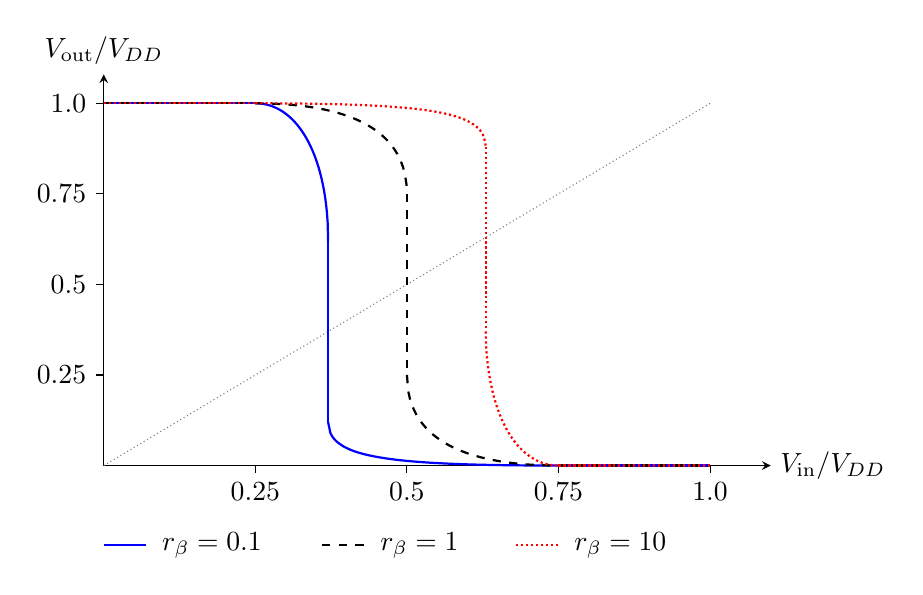
\begin{tikzpicture}[x=7.7cm,y=4.6cm,>=stealth,
 lowratio/.style={blue,thick},
 balancedratio/.style={black,thick,dashed},
 highratio/.style={red,thick,densely dotted}]
\draw[->] (0,0)--(1.10,0) node[right] {\(V_{\mathrm{in}}/V_{DD}\)};
\draw[->] (0,0)--(0,1.08) node[above] {\(V_{\mathrm{out}}/V_{DD}\)};
\foreach \x in {0.25,0.5,0.75,1.0}
 {\draw (\x,0)--(\x,-0.02) node[below] {\(\x\)};}
\foreach \y in {0.25,0.5,0.75,1.0}
 {\draw (0,\y)--(-0.013,\y) node[left] {\(\y\)};}
\draw[densely dotted,gray] (0,0)--(1,1);
\foreach \r/\curvestyle in {0.1/lowratio,1/balancedratio,10/highratio} {
 \pgfmathsetmacro{\m}{(0.25+sqrt(\r)*0.75)/(1+sqrt(\r))}
 \draw[\curvestyle] (0,1)--(0.25,1);
 \draw[\curvestyle,domain=0.25:\m,samples=100]
  plot (\x,{\x+0.25+sqrt(max(0,(0.75-\x)^2-(\x-0.25)^2/\r))})
  -- (\m,{\m+0.25});
 \draw[\curvestyle] (\m,{\m+0.25})--(\m,{\m-0.25});
 \draw[\curvestyle,domain=\m:0.75,samples=100]
  plot (\x,{\x-0.25-sqrt(max(0,(\x-0.25)^2-\r*(0.75-\x)^2))});
 \draw[\curvestyle] (0.75,0)--(1,0);
}
\draw[blue,thick] (0,-0.22)--(0.07,-0.22);
\node[anchor=west] at (0.08,-0.22) {\(r_\beta=0.1\)};
\draw[black,thick,dashed] (0.36,-0.22)--(0.43,-0.22);
\node[anchor=west] at (0.44,-0.22) {\(r_\beta=1\)};
\draw[red,thick,densely dotted] (0.68,-0.22)--(0.75,-0.22);
\node[anchor=west] at (0.76,-0.22) {\(r_\beta=10\)};
\end{tikzpicture}
\end{latin}
\caption{جابه‌جایی مشخصه انتقال با تغییر نسبت \lr{Beta} در مدل
مربعی ایده‌آل. محورها بی‌بعدند و خط مورب شرط
\(V_{\mathrm{out}}=V_{\mathrm{in}}\) را مشخص می‌کند.}
\label{fig:beta-vtc-family}
\end{figure}

\subsubsection{استخراج آستانه در حد \lr{Velocity Saturation}}
\label{sec:beta-velocity-limit}
در حد اشباع کامل سرعت، رابطه \secnum{۲.۲۹} کتاب جریان اشباع
را تقریباً متناسب با توان اول اضافه‌ولتاژ می‌دهد. با تعریف
\(K_n=W_nC_{\mathrm{ox},n}v_{\mathrm{sat},n}\) و
\(K_p=W_pC_{\mathrm{ox},p}v_{\mathrm{sat},p}\)، بزرگی دو جریان
رابطه \secnum{۲.۵۶} کتاب چنین نوشته می‌شود
\begin{equation}
 I_n=K_n(M-L),\qquad I_p=K_p(H-M).
 \label{eq:beta-velocity-currents}
\end{equation}
واحد \(K\) از حاصل‌ضرب
\(\mathrm{m}\times\mathrm{F\,m^{-2}}\times\mathrm{m\,s^{-1}}\)
برابر \(\mathrm{F\,s^{-1}}=\mathrm{A\,V^{-1}}\) است.
پس ضرب آن در ولتاژ، جریان می‌دهد.
این حد وقتی قابل استفاده است که محدودیت سرعت غالب باشد.
در \NotesTopic{sec:high-field}{مدل میدان قوی}، شرط متناظر
\(V_c\ll V_{GT}\) است و باید برای هر افزاره بررسی شود.

نسبت قدرت در این مدل را با نماد متمایز تعریف می‌کنیم
\begin{equation}
 \boxed{r_v=\frac{K_p}{K_n}
 =\frac{W_pC_{\mathrm{ox},p}v_{\mathrm{sat},p}}
        {W_nC_{\mathrm{ox},n}v_{\mathrm{sat},n}}}>0.
 \label{eq:beta-velocity-ratio}
\end{equation}
در فرض عایق گیت یکسان، \(C_{\mathrm{ox}}\) حذف می‌شود و همان
تعریف \(r=W_pv_{\mathrm{sat},p}/(W_nv_{\mathrm{sat},n})\)
صفحه ۹۰ کتاب به دست می‌آید. کتاب نماد \(r\) را در این مرحله
دوباره تعریف می‌کند. این جزوه از \(r_\beta\) و \(r_v\) استفاده
می‌کند تا مدل هر نسبت روشن باشد.

با برابرکردن جریان‌ها و تقسیم بر \(K_n>0\)، مراحل حل عبارت‌اند از
\begin{align}
 M-L&=r_v(H-M),\notag\\
 M+r_vM&=L+r_vH,\notag\\
 \boxed{M=\frac{L+r_vH}{1+r_v}
 =\frac{V_{tn}+r_v(V_{DD}-V_{TP})}{1+r_v}}.
 \label{eq:beta-velocity-threshold}
\end{align}
با تقسیم صورت و مخرج بر \(r_v\)، شکل رابطه \secnum{۲.۵۷}
کتاب حاصل می‌شود
\begin{equation}
 M=\frac{V_{DD}+V_{tp}+V_{tn}/r_v}{1+1/r_v}.
 \label{eq:beta-book-velocity-form}
\end{equation}
شرط دامنه نیز با
\(M-L=r_v\Delta/(1+r_v)>0\) و
\(H-M=\Delta/(1+r_v)>0\) تأیید می‌شود.
در \(r_v=1\) و آستانه‌های برابر، دوباره
\(M=V_{DD}/2\) است.

\paragraph*{مثال آموزشی مدل خطی اضافه‌ولتاژ}
فرض کنید حد اشباع کامل سرعت برای هر دو افزاره برقرار باشد،
\(V_{DD}=\qty{1.2}{\volt}\)،
\(V_{tn}=V_{TP}=\qty{0.3}{\volt}\)،
\(K_n=\qty{50}{\micro\ampere\per\volt}\) و
\(K_p=\qty{200}{\micro\ampere\per\volt}\).
این پارامترها یک مدل آموزشی مستقل را تعریف می‌کنند.
در \(r_v=4\)، داریم
\begin{equation*}
 M=\frac{0.3+4(0.9)}{5}=\qty{0.78}{\volt}.
\end{equation*}
اضافه‌ولتاژها \(\qty{0.48}{\volt}\) و \(\qty{0.12}{\volt}\) هستند.
برابری جریان‌ها با جای‌گذاری این دو مقدار کنترل می‌شود.
\[
 50(0.48)=200(0.12)=\qty{24}{\micro\ampere}.
\]
ولتاژهای \(V_{DS,n}=\qty{0.78}{\volt}\) و
\(V_{SD,p}=\qty{0.42}{\volt}\) از اضافه‌ولتاژهای متناظر بیشترند.
فرض محدودیت غالب سرعت، بخشی از مدل این مثال است.
تأیید آن در یک فناوری به پارامترهای \(V_c\) همان فناوری نیاز دارد.

\subsubsection{مقایسه حساسیت دو مدل و طراحی ابعاد}
\label{sec:beta-sensitivity-sizing}
جدول \ref{tab:beta-threshold-comparison} آستانه را با
\(L=\qty{0.3}{\volt}\) و \(H=\qty{0.9}{\volt}\) مقایسه می‌کند.
عدد نسبت در هر ستون، با تعریف همان مدل به کار رفته است.
قرارگرفتن دو مقدار برابر در یک ردیف، انتخاب آموزشی وزن‌های
بی‌بعد است. برای یک هندسه مشخص، باید هر نسبت جداگانه از
پارامترهای همان مدل محاسبه شود.
\begin{table}[!htbp]
\centering
\small
\caption{آستانه محاسبه‌شده از دو مدل برای نسبت‌های فرضی.
هر دو ستون آستانه برحسب \(\unit{\volt}\) هستند.}
\label{tab:beta-threshold-comparison}
\begin{tabular}{ccc}
\toprule
مقدار نسبت در مدل مربوط & \(M(r_\beta)\)، مدل مربعی & \(M(r_v)\)، حد سرعت\\
\midrule
\num{0.1} & \num{0.4442} & \num{0.3545}\\
\num{0.5} & \num{0.5485} & \num{0.5000}\\
\num{1} & \num{0.6000} & \num{0.6000}\\
\num{2} & \num{0.6515} & \num{0.7000}\\
\num{4} & \num{0.7000} & \num{0.7800}\\
\num{10} & \num{0.7558} & \num{0.8455}\\
\bottomrule
\end{tabular}
\end{table}

\paragraph*{استخراج حساسیت نزدیک نسبت یک}
مشتق \(\mathrm{d}M/\mathrm{d}r\)، تغییر آستانه در برابر تغییر
کوچک نسبت را اندازه می‌گیرد. برای مدل مربعی،
\(M=L+\Delta s/(1+s)\) و \(s=\sqrt{r_\beta}\) است.
مشتق \(s/(1+s)\) نسبت به \(s\) و مشتق ریشه به‌ترتیب چنین‌اند.
\[
 \frac{(1+s)-s}{(1+s)^2}=\frac{1}{(1+s)^2},\qquad
 \frac{\mathrm{d}s}{\mathrm{d}r_\beta}=\frac{1}{2\sqrt{r_\beta}}.
\]
با ضرب این دو نرخ، نتیجه می‌شود
\begin{equation}
 \frac{\mathrm{d}M}{\mathrm{d}r_\beta}
 =\frac{\Delta}{2\sqrt{r_\beta}(1+\sqrt{r_\beta})^2},\qquad
 \left.\frac{\mathrm{d}M}{\mathrm{d}r_\beta}\right|_{r_\beta=1}
 =\frac{\Delta}{8}.
 \label{eq:beta-long-sensitivity}
\end{equation}
برای مدل حد سرعت، \(M=L+\Delta r_v/(1+r_v)\) است، پس
\begin{equation}
 \frac{\mathrm{d}M}{\mathrm{d}r_v}
 =\frac{\Delta}{(1+r_v)^2},\qquad
 \left.\frac{\mathrm{d}M}{\mathrm{d}r_v}\right|_{r_v=1}
 =\frac{\Delta}{4}.
 \label{eq:beta-velocity-sensitivity}
\end{equation}
هر دو مشتق مثبت و دارای واحد ولت‌اند، زیرا نسبت بی‌بعد است.
در مقایسه حول نسبت یک و برای \(\Delta\) یکسان، حساسیت حد سرعت
دو برابر حساسیت مدل مربعی است. با \(\Delta=\qty{0.6}{\volt}\)،
شیب‌ها \(\qty{0.075}{\volt}\) و \(\qty{0.15}{\volt}\) به ازای
یک واحد تغییر نسبت‌اند. برای افزایش نسبت از یک به \num{1.1}،
تقریب خطی به‌ترتیب جابه‌جایی \(\qty{7.5}{\milli\volt}\) و
\(\qty{15}{\milli\volt}\) می‌دهد. محاسبه دقیق،
\(\qty{7.147}{\milli\volt}\) و
\(\qty{14.286}{\milli\volt}\) است.

مرجع حساسیت بیشتر مدارهای با محدودیت سرعت به \lr{Skew} را بیان
می‌کند \cite[پایان صفحه ۹۰]{weste}. مشتق‌های حاضر، این موضوع
را برای آستانه و نسبت‌های تعریف‌شده کمی می‌کنند.
شیب منحنی انتقال نسبت به ورودی، کمیت دیگری است و از
\eqref{eq:inverter-gain} و رسانایی‌های خروجی اثر می‌گیرد.
هر دو مدل ایده‌آل اشباع در استخراج آستانه، مستقل از خروجی‌اند و
در ناحیه اشباع هم‌زمان، گذار عمودی دارند. برای توصیف شیب محدود
مدار واقعی باید اثرهایی مانند \lr{CLM} نیز وارد شوند.

\paragraph*{از نسبت قدرت تا نسبت عرض}
رابطه هندسی مدل مربعی به صورت زیر است
\begin{equation}
 r_\beta=\frac{\mu_pC_{\mathrm{ox},p}}{\mu_nC_{\mathrm{ox},n}}
          \frac{W_p/L_p}{W_n/L_n}.
 \label{eq:beta-geometry-ratio}
\end{equation}
در طول و عایق یکسان،
\(r_\beta=(\mu_p/\mu_n)(W_p/W_n)\).
برای مثال فرضی \(\mu_p=0.5\mu_n\)، نسبت عرض دو،
\(r_\beta=1\) و نسبت عرض هشت، \(r_\beta=4\) می‌دهد.
کتاب معمولاً تغییر عرض با نگه‌داشتن طول کمینه مناسب فناوری را
برای تنظیم \lr{Skew} مطرح می‌کند \cite[صفحه ۹۰]{weste}.
تغییر طول هم‌زمان بر جریان، ظرفیت و اثرهای کانال کوتاه اثر دارد.
مقادیر ابعاد باید با تعریف ابعاد مؤثر مدل سازگار باشند.

در حد سرعت و با عایق یکسان،
\(r_v=(v_{\mathrm{sat},p}/v_{\mathrm{sat},n})(W_p/W_n)\).
اگر به‌طور آموزشی \(v_{\mathrm{sat},p}=0.8v_{\mathrm{sat},n}\)
و \(W_p/W_n=2\) فرض شوند، \(r_v=1.6\) است.
با \(\mu_p/\mu_n=0.5\)، همین نسبت عرض در مدل مربعی
\(r_\beta=1\) داشت. برای آستانه‌های \(\qty{0.3}{\volt}\) و
تغذیه \(\qty{1.2}{\volt}\)، نتیجه رسمی مدل مربعی
\(M=\qty{0.6}{\volt}\) است. محاسبه در حد سرعت می‌دهد
\[
 M=\frac{0.3+1.6\times0.9}{2.6}\approx\qty{0.6692}{\volt}.
\]
برای کاربرد هر حد باید دامنه اعتبار آن بررسی شود.

\paragraph*{طراحی معکوس برای آستانه مطلوب}
اگر آستانه هدف \(M_\star\) در \(L<M_\star<H\) باشد، از
\eqref{eq:beta-positive-root} و مدل حد سرعت به دست می‌آید
\begin{equation}
 \boxed{r_\beta=\left(\frac{M_\star-L}{H-M_\star}\right)^2},\qquad
 \boxed{r_v=\frac{M_\star-L}{H-M_\star}}.
 \label{eq:beta-inverse-sizing}
\end{equation}
هر دو کسر بی‌بعد و مثبت‌اند. نزدیک‌شدن هدف به \(H\)، مخرج را
کوچک و نسبت مورد نیاز را بزرگ می‌کند.
برای \(M_\star=\qty{0.65}{\volt}\)، \(L=\qty{0.3}{\volt}\)
و \(H=\qty{0.9}{\volt}\)، نسبت اضافه‌ولتاژها چنین محاسبه می‌شود.
\[
 \frac{0.65-0.3}{0.9-0.65}=\frac{0.35}{0.25}=1.4.
\]
پس \(r_\beta=1.96\) و \(r_v=1.4\) لازم است.
در مدل مربعی با \(\mu_p/\mu_n=0.5\)، طول و عایق یکسان،
نسبت عرض‌ها به دست می‌آید.
\[
 \frac{W_p}{W_n}=\frac{1.96}{0.5}=3.92.
\]
اگر \(W_n=\qty{0.4}{\micro\metre}\)،
\(W_p=\qty{1.568}{\micro\metre}\) خواهد بود.
این ابعاد، نتیجه مدل آموزشی‌اند و گردکردن ابعاد واقعی تابع قواعد
فناوری است. افزایش عرض، ظرفیت و مساحت را هم تغییر می‌دهد.

\subsubsection{تبدیل گیت‌های دیگر به \lr{Equivalent Inverter}}
\label{sec:beta-equivalent-inverter}
انتهای بخش \secnum{۲.۵.۲} کتاب و اسلاید ۸، تحلیل گیت‌های دیگر
با یک \lr{Equivalent Inverter} را مطرح می‌کنند
\cite[صفحه ۹۰ و آغاز ۹۱]{weste}\cite[اسلاید ۸]{dcslides}.
ابتدا ورودی‌های ثابت و متغیر و مسیرهای روشن را مشخص می‌کنیم.
چند ترانزیستور موازی روشن با بایاس‌های یکسان، جریان‌هایشان را جمع
می‌کنند و در مدل ساده، عرض مؤثر بیشتری می‌دهند. اگر تنها یک
شاخه موازی روشن باشد، شاخه‌های خاموش در جریان هدایت ایده‌آل
سهم صفر دارند. ظرفیت و نشتی آن شاخه‌ها در تحلیل‌های مربوط به
خود همچنان مطرح‌اند.

برای افزاره‌های یکسان موازی با گیت مشترک،
\(\beta_{\mathrm{eq}}=m\beta\) است که \(m\) تعداد واحدهای روشن
است. برای \(m\) واحد یکسان سری با گیت مشترک، در مدل
\lr{Shockley} با آستانه ثابت و بدون اثر بدنه و \lr{CLM}،
معادل طول \(mL_n\) یا \(mL_p\) و ضریب
\(\beta_{\mathrm{eq}}=\beta/m\) به کار می‌رود.
این نتیجه با برابری جریان‌ها و جمع افت ولتاژهای کانال سازگار است.
در مدل‌های غیرایده‌آل، به‌ویژه با اثر بدنه و محدودیت سرعت،
باید ناحیه کاری و گره‌های داخلی دوباره بررسی شوند.

\paragraph*{پیش‌نیاز \lr{NAND} و \lr{NOR}}
گیت دوورودی \lr{NAND}، متمم \lr{AND} است. خروجی فقط وقتی
صفر می‌شود که هر دو ورودی یک باشند. گیت \lr{NOR}، متمم
\lr{OR} است و خروجی فقط وقتی یک می‌شود که هر دو ورودی صفر
باشند. در پیاده‌سازی \lr{Static CMOS}، \lr{NAND} دو
\lr{nMOS} سری در شبکه پایین‌کش و دو \lr{pMOS} موازی در
شبکه بالاکش دارد. \lr{NOR} دو \lr{nMOS} موازی و دو
\lr{pMOS} سری دارد \cite[فصل ۱، بخش \secnum{۱.۴}]{weste}.
در مثال آموزشی حاضر، دو ورودی هر گیت به یک ولتاژ مشترک
\(v\) وصل می‌شوند تا مشخصه \(y(v)\) تک‌ورودی تعریف شود.

فرض کنید همه \lr{nMOS}ها ضریب \(\beta_n\) و همه
\lr{pMOS}ها ضریب \(\beta_p\) داشته باشند. با مدل سری و
موازی بیان‌شده، جدول \ref{tab:beta-equivalent-gates} حاصل می‌شود.
\begin{table}[!htbp]
\centering
\small
\caption{معادل آموزشی گیت‌ها با هر دو ورودی متصل به \(v\).
اثر بدنه، نشتی و \lr{CLM} صفر و آستانه‌ها ثابت‌اند.}
\label{tab:beta-equivalent-gates}
\begin{tabular}{cccc}
\toprule
گیت & \(\beta_{n,\mathrm{eq}}\) & \(\beta_{p,\mathrm{eq}}\) & نسبت معادل\\
\midrule
\lr{Inverter} & \(\beta_n\) & \(\beta_p\) & \(r_\beta\)\\
\lr{NAND} دوورودی & \(\beta_n/2\) & \(2\beta_p\) & \(4r_\beta\)\\
\lr{NOR} دوورودی & \(2\beta_n\) & \(\beta_p/2\) & \(r_\beta/4\)\\
\bottomrule
\end{tabular}
\end{table}
برای نمونه فرضی با \(r_\beta=1\)،
\(V_{tn}=V_{TP}=\qty{0.3}{\volt}\) و
\(V_{DD}=\qty{1.2}{\volt}\)، نسبت \lr{NAND} برابر چهار و
آستانه آن \(\qty{0.7}{\volt}\) است.
نسبت \lr{NOR} برابر \num{0.25} است. آستانه آن از رابطه مدل محاسبه می‌شود.
\[
 \frac{0.3+0.5\times0.9}{1.5}=\qty{0.5}{\volt}.
\]
این مقایسه به اتصال هر دو ورودی به \(v\) و فرض‌های مدل وابسته
است. وقتی یک ورودی ثابت و دیگری متغیر باشد، ولتاژ گیت‌های
افزاره‌های سری یکسان نیست و معادل ساده باید با تحلیل مدار
همان حالت ارزیابی شود.

\subsubsection{تمرین‌های تشریحی و کنترل نهایی}
\label{sec:beta-practice}
\paragraph*{تمرین آموزشی ۱ و آستانه‌های نابرابر}
با \(V_{DD}=\qty{1.2}{\volt}\)،
\(V_{tn}=\qty{0.35}{\volt}\)،
\(V_{TP}=\qty{0.25}{\volt}\) و \(r_\beta=4\)، آستانه
ورودی را در مدل مربعی حساب کنید.

\textbf{پاسخ.}
\(L=\qty{0.35}{\volt}\)، \(H=\qty{0.95}{\volt}\) و
\(s=2\) هستند. بنابراین،
\[
 M=\frac{0.35+2\times0.95}{3}=\qty{0.75}{\volt}.
\]
اضافه‌ولتاژها \(\qty{0.4}{\volt}\) و
\(\qty{0.2}{\volt}\) می‌شوند و نسبت مربع آن‌ها چهار است.
در \(y=M\)، \(V_{DS,n}=\qty{0.75}{\volt}\) و
\(V_{SD,p}=\qty{0.45}{\volt}\) از اضافه‌ولتاژها بیشترند.
پس هر دو شرط اشباع برقرار و \lr{KCL} سازگار است.

\paragraph*{تمرین آموزشی ۲ و یک نسبت از دو کمیت متفاوت}
فرض کنید \(\beta_p/\beta_n=4\). آیا می‌توان همین عدد را در
رابطه \eqref{eq:beta-velocity-threshold} گذاشت؟

\textbf{پاسخ.}
رابطه مذکور به \(r_v=K_p/K_n\) نیاز دارد. مقدار آن از
عرض‌ها، \(C_{\mathrm{ox}}\) و سرعت‌های اشباع به دست می‌آید.
برای نمونه با عایق و طول یکسان،
\(\mu_p/\mu_n=0.5\) و \(W_p/W_n=8\)،
\(r_\beta=4\) می‌شود. اگر
\(v_{\mathrm{sat},p}/v_{\mathrm{sat},n}=0.8\) هم فرض شود،
\(r_v=6.4\) است. برای \(L=\qty{0.3}{\volt}\) و
\(H=\qty{0.9}{\volt}\)، محاسبه در حد سرعت می‌دهد
\[
 M=\frac{0.3+6.4\times0.9}{7.4}\approx\qty{0.8189}{\volt}.
\]
اعتبار حد سرعت باید برای افزاره‌های مسئله برقرار باشد.

\paragraph*{تمرین آموزشی ۳ و بررسی هدف طراحی}
برای \(L=\qty{0.3}{\volt}\) و \(H=\qty{0.9}{\volt}\)،
هدف \(M_\star=\qty{0.95}{\volt}\) را بررسی کنید.

\textbf{پاسخ.}
هدف از \(H\) بیشتر است. در آن ورودی، افزاره \lr{pMOS} در
مدل هدایت قوی خاموش است و فرض استخراج اشباع هم‌زمان برقرار
نیست. رابطه میانگین وزنی \eqref{eq:beta-long-threshold} برای
نسبت مثبت، جواب را در \(L<M<H\) قرار می‌دهد.
پس این هدف با تغییر نسبت مثبت در همین مدل قابل دستیابی نیست.
مربع‌کردن کسر منفی در فرمول معکوس، شرط دامنه را برطرف نمی‌کند.

بخش \secnum{۲.۵.۳}، ارتباط مشخصه انتقال با بازه‌های معتبر
منطقی و تحمل نویز را بررسی می‌کند.

% !TeX root = booklet-03.tex
\clearpage
\subsection{سطوح منطقی و \lr{Noise Margin}}
\label{sec:noise-margin}
خروجی یک گیت، ورودی گیت بعدی را تغذیه می‌کند. برای انتقال صحیح
داده، بازه ولتاژ تولیدشده در خروجی باید در بازه معتبر ورودی گیت
گیرنده قرار گیرد. نویز می‌تواند ولتاژ دریافتی را تغییر دهد.
\lr{Noise Margin} مقدار تغییر نامطلوبی را توصیف می‌کند که این
سازگاری را در شرایط تعریف‌شده حفظ می‌کند
\cite[بخش \secnum{۲.۵.۳}، صفحات ۹۱ و ۹۲]{weste}
\cite[اسلایدهای ۹ و ۱۰]{dcslides}.

\subsubsection{تعریف چهار سطح ولتاژ}
\label{sec:noise-logic-levels}
برای ورودی، \(V_{\mathrm{IL}}\) بیشترین ولتاژ پذیرفته‌شده به‌عنوان
\lr{LOW} و \(V_{\mathrm{IH}}\) کمترین ولتاژ پذیرفته‌شده به‌عنوان
\lr{HIGH} است. برای خروجی، \(V_{\mathrm{OL}}\) بیشترین ولتاژ
تولیدشده در حالت \lr{LOW} و \(V_{\mathrm{OH}}\) کمترین ولتاژ
تولیدشده در حالت \lr{HIGH} است. حرف \lr{I} به ورودی، حرف
\lr{O} به خروجی و حرف‌های \lr{L} و \lr{H} به سطح پایین و بالا
اشاره می‌کنند. جدول \ref{tab:noise-level-definitions} تعریف‌ها
را به شکل بازه نشان می‌دهد \cite[صفحه ۹۱]{weste}.
\begin{table}[!htbp]
\centering
\small
\caption{بازه‌های منطقی برای ولتاژهای بین زمین و تغذیه.
مرزهای ورودی به گیرنده و مرزهای خروجی به فرستنده مربوط‌اند.}
\label{tab:noise-level-definitions}
\begin{tabularx}{\linewidth}{cc>{\raggedleft\arraybackslash}X}
\toprule
پایانه & حالت & بازه معتبر\\
\midrule
ورودی & \lr{LOW} & \(0\le V_{\mathrm{in}}\le V_{\mathrm{IL}}\)\\
ورودی & \lr{HIGH} & \(V_{\mathrm{IH}}\le V_{\mathrm{in}}\le V_{DD}\)\\
خروجی & \lr{LOW} & \(0\le V_{\mathrm{out}}\le V_{\mathrm{OL}}\)\\
خروجی & \lr{HIGH} & \(V_{\mathrm{OH}}\le V_{\mathrm{out}}\le V_{DD}\)\\
\bottomrule
\end{tabularx}
\end{table}

بازه \(V_{\mathrm{IL}}<V_{\mathrm{in}}<V_{\mathrm{IH}}\) را
\lr{Indeterminate Region} یا \lr{Forbidden Zone} می‌نامند.
در این بازه، مشخصات منطقیِ تعریف‌شده، تفسیر معتبر صفر یا یک را
تضمین نمی‌کنند. مدار همچنان ولتاژ و جریان فیزیکی دارد و می‌توان
آن را با مشخصه انتقال تحلیل کرد.
\(V_{\mathrm{inv}}\) نیز نقطه \(V_{\mathrm{out}}=V_{\mathrm{in}}\)
از بخش \ref{sec:inverter-input-threshold} است. دو مرز
\(V_{\mathrm{IL}},V_{\mathrm{IH}}\) با معیار جداگانه‌ای تعیین
می‌شوند که در ادامه استخراج می‌شود.

در شرایط سازگار معمول، خروجی پایین باید از حداکثر ورودی پایین
کمتر و خروجی بالا باید از حداقل ورودی بالا بیشتر باشد. شکل
\ref{fig:noise-level-ranges} فاصله‌های مربوط را نشان می‌دهد.
\begin{figure}[!htbp]
\centering
\begin{latin}
\PersianMathDigits
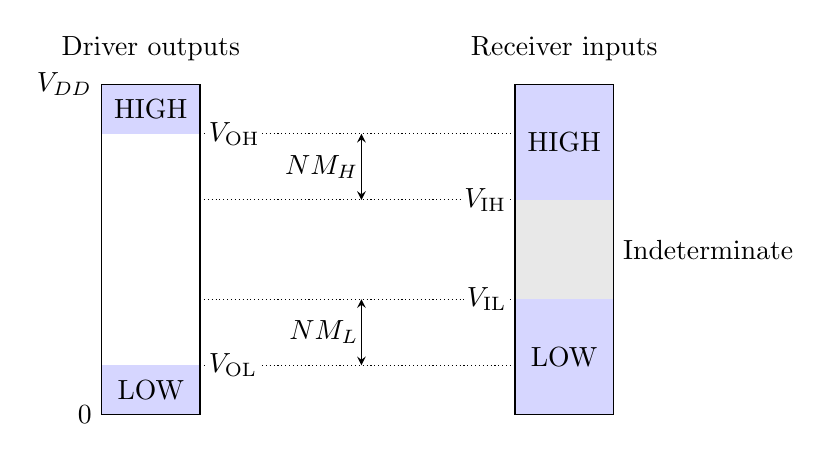
\begin{tikzpicture}[x=1cm,y=4.2cm,>=stealth]
\fill[blue!16] (0,0) rectangle (1.25,0.15);
\fill[blue!16] (0,0.85) rectangle (1.25,1);
\draw (0,0) rectangle (1.25,1);
\fill[blue!16] (5.25,0) rectangle (6.5,0.35);
\fill[gray!18] (5.25,0.35) rectangle (6.5,0.65);
\fill[blue!16] (5.25,0.65) rectangle (6.5,1);
\draw (5.25,0) rectangle (6.5,1);
\foreach \y in {0.15,0.35,0.65,0.85}
 {\draw[densely dotted] (1.25,\y)--(5.25,\y);}
\node[above] at (0.625,1.04) {Driver outputs};
\node[above] at (5.875,1.04) {Receiver inputs};
\node[left] at (0,0) {\(0\)};
\node[left] at (0,1) {\(V_{DD}\)};
\node at (0.625,0.075) {LOW};
\node at (0.625,0.925) {HIGH};
\node at (5.875,0.175) {LOW};
\node at (5.875,0.825) {HIGH};
\node[right] at (6.5,0.5) {Indeterminate};
\node[anchor=west,fill=white,inner sep=1pt] at (1.32,0.15) {\(V_{\mathrm{OL}}\)};
\node[anchor=west,fill=white,inner sep=1pt] at (1.32,0.85) {\(V_{\mathrm{OH}}\)};
\node[anchor=east,fill=white,inner sep=1pt] at (5.18,0.35) {\(V_{\mathrm{IL}}\)};
\node[anchor=east,fill=white,inner sep=1pt] at (5.18,0.65) {\(V_{\mathrm{IH}}\)};
\draw[<->] (3.3,0.15)--(3.3,0.35)
 node[midway,left,fill=white,inner sep=1pt] {\(NM_L\)};
\draw[<->] (3.3,0.65)--(3.3,0.85)
 node[midway,left,fill=white,inner sep=1pt] {\(NM_H\)};
\end{tikzpicture}
\end{latin}
\caption{طرح آموزشی بازه‌های ورودی و خروجی بر اساس شکل
\secnum{۲.۲۹} کتاب و اسلاید ۹. فاصله‌ها شماتیک‌اند و مقیاس
عددی یک فناوری را نمایش نمی‌دهند.}
\label{fig:noise-level-ranges}
\end{figure}

\subsubsection{استخراج حاشیه نویز از شرط سازگاری}
\label{sec:noise-margin-definition}
برای حالت پایین، بدترین خروجی مجاز فرستنده
\(V_{\mathrm{OL}}\) است. اگر نویز نامطلوب مثبت با بزرگی
\(v_n\ge0\) به آن اضافه شود، ولتاژ دریافتی در این حالت
\(V_{\mathrm{OL}}+v_n\) می‌شود. برای باقی‌ماندن در بازه
\lr{LOW} گیرنده، باید
\begin{equation*}
 V_{\mathrm{OL}}+v_n\le V_{\mathrm{IL}}
 \quad\Longrightarrow\quad
 v_n\le V_{\mathrm{IL}}-V_{\mathrm{OL}}.
\end{equation*}
پس رابطه \secnum{۲.۵۸} کتاب چنین تعریف می‌شود
\begin{equation}
 \boxed{NM_L=V_{\mathrm{IL}}-V_{\mathrm{OL}}}.
 \label{eq:noise-low-margin}
\end{equation}
برای حالت بالا، بدترین خروجی مجاز
\(V_{\mathrm{OH}}\) است. نویز نامطلوب، ولتاژ را کاهش می‌دهد.
شرط باقی‌ماندن ورودی در بازه \lr{HIGH} برابر است با
\begin{equation*}
 V_{\mathrm{OH}}-v_n\ge V_{\mathrm{IH}}
 \quad\Longrightarrow\quad
 v_n\le V_{\mathrm{OH}}-V_{\mathrm{IH}}.
\end{equation*}
در نتیجه، رابطه \secnum{۲.۵۹} کتاب چنین است
\begin{equation}
 \boxed{NM_H=V_{\mathrm{OH}}-V_{\mathrm{IH}}}.
 \label{eq:noise-high-margin}
\end{equation}
هر دو حاشیه واحد ولت دارند. وقتی بزرگی نویز در هر دو حالت
مهم باشد، کمیت \(\min(NM_L,NM_H)\) حاشیه محدودکننده را
نشان می‌دهد. مقدار صفر، فاصله اطمینان اضافی باقی نمی‌گذارد.
مقدار منفی یعنی حتی بدون نویز اضافه، همه خروجی‌های مجاز
فرستنده در بازه معتبر گیرنده قرار نمی‌گیرند.

\paragraph*{مثال آموزشی ارتباط دو گیت}
فرض کنید فرستنده \(V_{\mathrm{OL}}=\qty{0.1}{\volt}\) و
\(V_{\mathrm{OH}}=\qty{0.9}{\volt}\) و گیرنده
\(V_{\mathrm{IL}}=\qty{0.3}{\volt}\) و
\(V_{\mathrm{IH}}=\qty{0.7}{\volt}\) داشته باشند.
هر دو حاشیه \(\qty{0.2}{\volt}\) هستند.
نویز مثبت \(\qty{0.15}{\volt}\) روی بدترین سطح پایین،
ورودی \(\qty{0.25}{\volt}\) می‌دهد که هنوز معتبر است.
نویز کاهنده با همین بزرگی روی بدترین سطح بالا،
\(\qty{0.75}{\volt}\) می‌دهد که آن هم معتبر است.
اما با نویز مثبت \(\qty{0.25}{\volt}\)، سطح پایین به
\(\qty{0.35}{\volt}\) می‌رسد و وارد بازه نامعین می‌شود.
در این حالت، تضمین مشخصات منطقی از بین می‌رود. مقدار خروجی
واقعی باید از مشخصه گیرنده تعیین شود.

\subsubsection{معنای \lr{Unity Gain} و بدترین خروجی مجاز}
\label{sec:noise-unity-gain}
شیب مشخصه را با \(g\) نشان می‌دهیم. تعریف مشتق و تقریب تغییر کوچک
ورودی در همسایگی یک نقطه چنین‌اند.
\[
 g=\frac{\mathrm{d}V_{\mathrm{out}}}{\mathrm{d}V_{\mathrm{in}}},\qquad
 \Delta V_{\mathrm{out}}\approx g\Delta V_{\mathrm{in}}.
\]
مثلاً در \(g=-0.3\)، تغییر ورودی
\(\qty{10}{\milli\volt}\)، تقریباً
\(-\qty{3}{\milli\volt}\) تغییر خروجی ایجاد می‌کند.
در \(g=-4\)، همان تغییر ورودی حدود
\(-\qty{40}{\milli\volt}\) تغییر خروجی می‌دهد.
علامت منفی، رفتار معکوس‌کننده و بزرگی شیب، نسبت بزرگی تغییرها
را نشان می‌دهد.

نزدیک دو ریل، معمولاً \(|g|<1\) و در بخش میانی گذار،
\(|g|>1\) است. در قرارداد کتاب و اسلاید ۱۰، دو نقطه مرزی
با شرط زیر تعیین می‌شوند
\begin{equation}
 \boxed{g=-1}.
 \label{eq:noise-unity-condition}
\end{equation}
واژه \lr{Unity} به بزرگی یک اشاره دارد. چون مشخصه
\lr{Inverter} کاهشی است، مقدار علامت‌دار شیب منفی یک است.
نقطه سمت چپ، \(V_{\mathrm{IL}}\) و نقطه سمت راست،
\(V_{\mathrm{IH}}\) را مشخص می‌کند.
کتاب این مرزبندی را کرانی محافظه‌کارانه برای بدترین حاشیه نویز
ایستا توصیف می‌کند \cite[شکل \secnum{۲.۳۰} و صفحه ۹۲]{weste}.

در شاخه بالای یک مشخصه کاهشی، بیشترین ورودی پایین مجاز،
کمترین خروجی بالا را می‌دهد. در شاخه پایین، کمترین ورودی بالا
مجاز، بیشترین خروجی پایین را می‌دهد. بنابراین، برای همین
قرارداد سطوح منطقی می‌نویسیم
\begin{equation}
 V_{\mathrm{OH}}=V_{\mathrm{out}}(V_{\mathrm{IL}}),\qquad
 V_{\mathrm{OL}}=V_{\mathrm{out}}(V_{\mathrm{IH}}).
 \label{eq:noise-output-levels}
\end{equation}
در دو نقطه مرزی، خروجی می‌تواند کمی از ریل متناظر فاصله داشته
باشد. کتاب این انتقال اثر ورودی به خروجی را
\lr{Noise Feedthrough} یا \lr{Propagated Noise} می‌نامد
\cite[صفحه ۹۲]{weste}. این افت باید در تفاضل حاشیه‌ها لحاظ شود.

شکل \ref{fig:noise-unity-vtc} یک مثال آموزشی متقارن با
\(V_t=0.1V_{DD}\) است. روابط مدل مربعی بخش‌های قبل برای رسم
آن به کار رفته‌اند. در این مثال،
\(V_{\mathrm{IL}}=0.4V_{DD}\)،
\(V_{\mathrm{IH}}=0.6V_{DD}\)،
\(V_{\mathrm{OH}}=0.9V_{DD}\) و
\(V_{\mathrm{OL}}=0.1V_{DD}\) هستند.
\begin{figure}[!htbp]
\centering
\begin{latin}
\PersianMathDigits
\begin{tikzpicture}[x=8.4cm,y=5cm,>=stealth]
\draw[->] (0,0)--(1.1,0) node[right] {\(V_{\mathrm{in}}/V_{DD}\)};
\draw[->] (0,0)--(0,1.12) node[above] {\(V_{\mathrm{out}}/V_{DD}\)};
\draw[thick,blue] (0,1)--(0.1,1);
\draw[thick,blue,domain=0.1:0.5,samples=110]
 plot (\x,{\x+0.1+sqrt(max(0,(1-2*\x)*0.8))})--(0.5,0.6);
\draw[thick,blue] (0.5,0.6)--(0.5,0.4);
\draw[thick,blue,domain=0.5:0.9,samples=110]
 plot (\x,{\x-0.1-sqrt(max(0,(2*\x-1)*0.8))});
\draw[thick,blue] (0.9,0)--(1,0);
\draw[densely dotted] (0.4,0)--(0.4,0.9)--(0,0.9);
\draw[densely dotted] (0.6,0)--(0.6,0.1)--(0,0.1);
\draw[thick,red] (0.34,0.96)--(0.46,0.84);
\draw[thick,red] (0.54,0.16)--(0.66,0.04);
\fill (0.4,0.9) circle[radius=1.7pt];
\fill (0.6,0.1) circle[radius=1.7pt];
\node[below] at (0.4,0) {\(V_{\mathrm{IL}}/V_{DD}\)};
\node[below] at (0.6,0) {\(V_{\mathrm{IH}}/V_{DD}\)};
\node[below] at (1,0) {\(1\)};
\node[left] at (0,0.9) {\(V_{\mathrm{OH}}/V_{DD}\)};
\node[left] at (0,0.1) {\(V_{\mathrm{OL}}/V_{DD}\)};
\node[left] at (0,1) {\(1\)};
\node[above right] at (0.65,0.65) {\(g=-1\)};
\end{tikzpicture}
\end{latin}
\caption{نقاط \lr{Unity Gain} در مثال فرضی
\(V_t/V_{DD}=0.1\). پاره‌خط‌های قرمز مماس‌های با شیب منفی یک
در مختصات نرمال‌شده‌اند. ساخت شکل بر اساس شکل \secnum{۲.۳۰}
کتاب و اسلاید ۱۰ است.}
\label{fig:noise-unity-vtc}
\end{figure}

\subsubsection{پیش‌نیاز مشتق‌گیری و استخراج شیب دو شاخه}
\label{sec:noise-derivatives}
برای استخراج تحلیلی، مدل متقارن
\(\beta_n=\beta_p\)، \(V_{tn}=V_{TP}=V_t>0\) و
\(V_{DD}>2V_t\) را به کار می‌بریم. آستانه و \lr{Mobility}
ثابت و اثرهای نشتی و \lr{CLM} صفر فرض می‌شوند.
کمیت مثبت \(K=V_{DD}-2V_t\) را با واحد ولت تعریف می‌کنیم.
برای کوتاه‌شدن محاسبه، \(x=V_{\mathrm{in}}\) و
\(y=V_{\mathrm{out}}\) می‌گذاریم. روابط شاخه‌های \lr{B} و
\lr{D} از \eqref{eq:inverter-b-transfer} و
\eqref{eq:inverter-d-transfer} هستند.

مشتق یک مقدار ثابت نسبت به \(x\) صفر و مشتق خود \(x\) یک است.
برای ریشه، اگر \(z=\sqrt{u}>0\)، آنگاه \(z^2=u\).
مشتق‌گیری دو طرف نسبت به \(u\) می‌دهد
\[
 2z\frac{\mathrm{d}z}{\mathrm{d}u}=1
 \quad\Longrightarrow\quad
 \frac{\mathrm{d}\sqrt{u}}{\mathrm{d}u}=\frac{1}{2\sqrt{u}}.
\]
وقتی \(u\) خودش تابع \(x\) است، نرخ تغییر بیرونی را در نرخ
تغییر درونی ضرب می‌کنیم. این همان \lr{Chain Rule} است
\begin{equation}
 \frac{\mathrm{d}\sqrt{u(x)}}{\mathrm{d}x}
 =\frac{1}{2\sqrt{u(x)}}\frac{\mathrm{d}u}{\mathrm{d}x},
 \qquad u(x)>0.
 \label{eq:noise-chain-rule}
\end{equation}
این رابطه در شاخه‌های باز و دور از رادیکال صفر به کار می‌رود.

در شاخه \lr{B}، \(u(x)=K(V_{DD}-2x)\) و
\(\mathrm{d}u/\mathrm{d}x=-2K\) است. بنابراین،
\begin{align}
 y_B&=x+V_t+\sqrt{K(V_{DD}-2x)},\notag\\
 \frac{\mathrm{d}y_B}{\mathrm{d}x}
 &=1+\frac{-2K}{2\sqrt{K(V_{DD}-2x)}}\notag\\
 &=\boxed{1-\sqrt{\frac{K}{V_{DD}-2x}}}.
 \label{eq:noise-b-slope}
\end{align}
چون \(K>0\) و \(V_{DD}-2x>0\) در \lr{B}، تبدیل
\(K/\sqrt{K(V_{DD}-2x)}\) به ریشه نسبت، مجاز است.
نسبت داخل رادیکال بی‌بعد است، پس مشتق نیز بی‌بعد می‌شود.
شیب در ابتدای شاخه به صفر و هنگام نزدیک‌شدن به نقطه میانی
از چپ، به سمت مقادیر منفی با بزرگی زیاد می‌رود.

در شاخه \lr{D}، \(u(x)=K(2x-V_{DD})\) و
\(\mathrm{d}u/\mathrm{d}x=2K\) است. علامت منفی جلوی ریشه را
هم حفظ می‌کنیم
\begin{align}
 y_D&=x-V_t-\sqrt{K(2x-V_{DD})},\notag\\
 \frac{\mathrm{d}y_D}{\mathrm{d}x}
 &=1-\frac{2K}{2\sqrt{K(2x-V_{DD})}}\notag\\
 &=\boxed{1-\sqrt{\frac{K}{2x-V_{DD}}}}.
 \label{eq:noise-d-slope}
\end{align}
در این شاخه نیز رادیکال مثبت است. شیب از بزرگی زیاد نزدیک
گذار میانی به صفر در انتهای شاخه نزدیک می‌شود.

\subsubsection{استخراج چهار سطح در مدل متقارن}
\label{sec:noise-symmetric-levels}
با گذاشتن \(x=V_{\mathrm{IL}}\) و شیب منفی یک در
\eqref{eq:noise-b-slope}، داریم
\begin{align}
 1-\sqrt{\frac{K}{V_{DD}-2V_{\mathrm{IL}}}}&=-1,\notag\\
 \sqrt{\frac{K}{V_{DD}-2V_{\mathrm{IL}}}}&=2,\notag\\
 V_{DD}-2V_{\mathrm{IL}}&=\frac{K}{4},\notag\\
 \boxed{V_{\mathrm{IL}}=\frac{3V_{DD}+2V_t}{8}}.
 \label{eq:noise-vil}
\end{align}
ریشه سمت چپ مثبت است و برابر دو قرار داده شده است. با
مربع‌کردن، عدد چهار به دست می‌آید. حل سطر سوم و جای‌گذاری
\(K=V_{DD}-2V_t\)، سطر نهایی را می‌دهد.

با گذاشتن \(x=V_{\mathrm{IH}}\) در شاخه \lr{D}، به همین ترتیب
\begin{align}
 1-\sqrt{\frac{K}{2V_{\mathrm{IH}}-V_{DD}}}&=-1,\notag\\
 2V_{\mathrm{IH}}-V_{DD}&=\frac{K}{4},\notag\\
 \boxed{V_{\mathrm{IH}}=\frac{5V_{DD}-2V_t}{8}}.
 \label{eq:noise-vih}
\end{align}
برای کنترل دامنه، تفاضل با مرزهای شاخه را محاسبه می‌کنیم
\begin{align*}
 V_{\mathrm{IL}}-V_t
 &=V_{DD}-V_t-V_{\mathrm{IH}}=\frac{3K}{8}>0,\\
 \frac{V_{DD}}{2}-V_{\mathrm{IL}}
 &=V_{\mathrm{IH}}-\frac{V_{DD}}{2}=\frac{K}{8}>0.
\end{align*}
پس \(V_{\mathrm{IL}}\) واقعاً داخل \lr{B} و
\(V_{\mathrm{IH}}\) داخل \lr{D} است. هیچ‌یک روی پاره‌خط
عمودی ناحیه \lr{C} قرار ندارد.

در هر نقطه مرزی، مقدار رادیکال با شرط مثبت‌بودن \(K\) محاسبه می‌شود.
\[
 \sqrt{K(K/4)}=K/2,\qquad K>0.
\]
با استفاده از \eqref{eq:noise-output-levels}، سطوح خروجی به
دست می‌آیند
\begin{align}
 V_{\mathrm{OH}}&=V_{\mathrm{IL}}+V_t+\frac{K}{2}
 =\boxed{\frac{7V_{DD}+2V_t}{8}},\notag\\
 V_{\mathrm{OL}}&=V_{\mathrm{IH}}-V_t-\frac{K}{2}
 =\boxed{\frac{V_{DD}-2V_t}{8}}.
 \label{eq:noise-voh-vol}
\end{align}
بنابراین، افت خروجی در مرزهای ورودی مجاز چنین است.
\[
 V_{DD}-V_{\mathrm{OH}}=V_{\mathrm{OL}}=K/8.
\]
در این دامنه، افت مثبت است.
حاشیه‌ها با تفاضل سطوح محاسبه می‌شوند
\begin{align}
 NM_L&=\frac{3V_{DD}+2V_t}{8}-\frac{V_{DD}-2V_t}{8}
 =\frac{V_{DD}+2V_t}{4},\notag\\
 NM_H&=\frac{7V_{DD}+2V_t}{8}-\frac{5V_{DD}-2V_t}{8}
 =\frac{V_{DD}+2V_t}{4}.
 \label{eq:noise-symmetric-margins}
\end{align}
پس دو حاشیه برابرند. روابط
\(V_{\mathrm{IL}}+V_{\mathrm{IH}}=V_{DD}\) و
\(V_{\mathrm{OL}}+V_{\mathrm{OH}}=V_{DD}\) نیز تقارن را
تأیید می‌کنند. عرض بازه نامعین در این مدل برابر است با
\(V_{\mathrm{IH}}-V_{\mathrm{IL}}=K/4\).

\subsubsection{حل کامل تمرین \secnum{۲.۱۷}}
\label{sec:noise-ex17}
صورت اصلی تمرین، استفاده از نتایج تمرین \secnum{۲.۱۶} برای محاسبه
حاشیه نویز یک \lr{CMOS Inverter} با تغذیه
\(\qty{1.0}{\volt}\)، آستانه‌های
\(V_{tn}=|V_{tp}|=\qty{0.35}{\volt}\) و
\(\beta_n=\beta_p\) را می‌خواهد
\cite[تمرین \secnum{۲.۱۷}، صفحه چاپی ۹۷]{weste}.
روابط انتقال لازم پیش‌تر در بخش
\ref{sec:inverter-five-regions} استخراج شده‌اند.
همان مدل \lr{Shockley}، آستانه ثابت، بدنه متصل به سورس و
بار بدون جریان \lr{DC} را به کار می‌بریم. اثرهای نشتی و
\lr{CLM} در مدل این تمرین صفرند.

ابتدا پارامتر \(K\) را محاسبه و علامت آن را کنترل می‌کنیم.
\[
 K=1.0-2(0.35)=\qty{0.30}{\volt}>0.
\]
پس فرض وجود شاخه‌های \lr{B} و \lr{D} برقرار است.
با جای‌گذاری در روابط استخراج‌شده، داریم
\begin{align*}
 V_{\mathrm{IL}}&=\frac{3(1.0)+2(0.35)}{8}
 =\qty{0.4625}{\volt},\\
 V_{\mathrm{IH}}&=\frac{5(1.0)-2(0.35)}{8}
 =\qty{0.5375}{\volt},\\
 V_{\mathrm{OH}}&=\frac{7(1.0)+2(0.35)}{8}
 =\qty{0.9625}{\volt},\\
 V_{\mathrm{OL}}&=\frac{1.0-2(0.35)}{8}
 =\qty{0.0375}{\volt}.
\end{align*}
ارقام اعشاری برای بازبینی محاسبه مدل حفظ شده‌اند.
این تعداد رقم، دقت فیزیکی یک فناوری را تعیین نمی‌کند.
تفاضل‌های لازم می‌دهند
\begin{equation*}
 \boxed{NM_L=0.4625-0.0375=\qty{0.425}{\volt}},\qquad
 \boxed{NM_H=0.9625-0.5375=\qty{0.425}{\volt}}.
\end{equation*}
هر حاشیه \num{42.5} درصد تغذیه است.
در صورت گزارش با دو رقم اعشار و قاعده گردکردن نیم‌به‌بالا،
\(\qty{0.43}{\volt}\) حاصل می‌شود. محاسبه اصلی با مقادیر
گردنشده انجام می‌شود. اگر چهار سطح را ابتدا به دو رقم اعشار
گرد کنیم، تفاضل \(0.46-0.04=\qty{0.42}{\volt}\) به دست
می‌آید. این مثال اثر گردکردن میانی را نشان می‌دهد.

\paragraph*{کنترل جریان و ناحیه کاری در نقطه چپ}
در \(V_{\mathrm{in}}=\qty{0.4625}{\volt}\) و
\(V_{\mathrm{out}}=\qty{0.9625}{\volt}\)،
اضافه‌ولتاژها \(a=\qty{0.1125}{\volt}\) و
\(b=\qty{0.1875}{\volt}\) هستند.
\(V_{DS,n}=\qty{0.9625}{\volt}>a\)، پس \lr{nMOS} در
اشباع است. \(V_{SD,p}=\qty{0.0375}{\volt}<b\)، پس
\lr{pMOS} در \lr{Linear} است.
چون مقدار عددی \(\beta\) در صورت مسئله داده نشده است،
جریان‌ها را بر \(\beta\) تقسیم می‌کنیم
\begin{align}
 \frac{I_n}{\beta}&=\frac{(0.1125)^2}{2}
 =\qty{0.006328125}{\volt\squared},\notag\\
 \frac{I_p}{\beta}&=(0.1875)(0.0375)-\frac{(0.0375)^2}{2}
 =\qty{0.006328125}{\volt\squared}.
 \label{eq:noise-ex17-kcl}
\end{align}
واحد نسبت، آمپر تقسیم بر آمپر بر ولت مربع و برابر ولت مربع است.
برابری دو نسبت، \lr{KCL} را برای هر \(\beta>0\) تأیید می‌کند.
شیب نیز از \eqref{eq:noise-b-slope} به دست می‌آید.
\[
 1-\sqrt{\frac{0.30}{1-2\times0.4625}}=1-2=-1.
\]

\paragraph*{کنترل نقطه راست و حاشیه‌ها}
در \(V_{\mathrm{in}}=\qty{0.5375}{\volt}\)، خروجی
\(\qty{0.0375}{\volt}\)، اضافه‌ولتاژ \lr{nMOS}
\(\qty{0.1875}{\volt}\) و اضافه‌ولتاژ \lr{pMOS}
\(\qty{0.1125}{\volt}\) است.
بنابراین \lr{nMOS} در \lr{Linear} و \lr{pMOS} در اشباع
قرار می‌گیرند. دو نسبت جریان، همان مقدار
\eqref{eq:noise-ex17-kcl} را دارند. محاسبه شیب می‌دهد
\[
 1-\sqrt{\frac{0.30}{0.075}}=-1.
\]
همچنین ترتیب چهار سطح تأیید می‌شود.
\[
 0.0375<0.4625<0.5375<0.9625.
\]
در بدترین سطح پایین، افزودن
\(\qty{0.425}{\volt}\)، ورودی را دقیقاً به
\(\qty{0.4625}{\volt}\) می‌رساند.
در بدترین سطح بالا، کم‌کردن همین مقدار،
\(\qty{0.5375}{\volt}\) می‌دهد. هر دو، روی مرز مجاز قرار دارند.

\subsubsection{اثر \lr{Skew}، آستانه و مقیاس تغذیه}
\label{sec:noise-skew-tradeoff}
کتاب بیان می‌کند که در حالت متقارن، دو حاشیه برابرند و این
تعادل برای نویز با جهت نامشخص مطلوب است. اگر یک حالت منطقی
بیشتر در معرض نویز باشد، با \lr{Skew} می‌توان حاشیه آن را
بهبود داد و تغییر حاشیه دیگر را نیز باید پذیرفت
\cite[صفحه ۹۲]{weste}.

برای محاسبه در مدل مربعی نامتقارن، می‌توان از شاخه‌های
\eqref{eq:beta-b-transfer} و \eqref{eq:beta-d-transfer} استفاده
کرد. چون \(\mathrm{d}a/\mathrm{d}x=1\) و
\(\mathrm{d}b/\mathrm{d}x=-1\)، همان \lr{Chain Rule} می‌دهد
\begin{equation}
 g_B=1-\frac{b+a/r_\beta}{\sqrt{b^2-a^2/r_\beta}},\qquad
 g_D=1-\frac{a+r_\beta b}{\sqrt{a^2-r_\beta b^2}}.
 \label{eq:noise-skew-slopes}
\end{equation}
برای نمونه، مشتق رادیکال شاخه \lr{B} به صورت زیر نوشته می‌شود.
\[
 \frac{-2b-2a/r_\beta}{2\sqrt{b^2-a^2/r_\beta}}.
\]
در هر شاخه، ریشه \(g=-1\) را در دامنه همان شاخه پیدا
می‌کنیم، سپس خروجی‌های متناظر را محاسبه می‌کنیم.
جدول \ref{tab:noise-skew-example} نتیجه حل عددی این شرط را
برای سه نسبت فرضی، با تغذیه \(\qty{1}{\volt}\) و آستانه‌های
برابر \(\qty{0.35}{\volt}\)، نشان می‌دهد.
\begin{table}[!htbp]
\centering
\small
\caption{مقایسه حاشیه‌های مدل مربعی با \lr{Skew} فرضی.
همه ولتاژها برحسب \(\unit{\volt}\) و مقادیر تا چهار رقم اعشار گرد شده‌اند.}
\label{tab:noise-skew-example}
\begin{tabular}{cccccc}
\toprule
\(r_\beta\) & \(V_{\mathrm{IL}}\) & \(V_{\mathrm{IH}}\) &
\(NM_L\) & \(NM_H\) & کمترین حاشیه\\
\midrule
\num{0.5} & \num{0.4295} & \num{0.5036} & \num{0.3893} & \num{0.4657} & \num{0.3893}\\
\num{1} & \num{0.4625} & \num{0.5375} & \num{0.4250} & \num{0.4250} & \num{0.4250}\\
\num{2} & \num{0.4964} & \num{0.5705} & \num{0.4657} & \num{0.3893} & \num{0.3893}\\
\bottomrule
\end{tabular}
\end{table}
در این نمونه، تقویت \lr{pMOS}، حاشیه پایین را افزایش و حاشیه
بالا را کاهش داده است. \(NM_L\) به تحمل افزایش ولتاژ روی سطح
پایین مربوط است. \(NM_H\) به تحمل کاهش ولتاژ روی سطح بالا
مربوط می‌شود. انتخاب نسبت باید با نوع نویز و نیاز مدار سازگار باشد.
مقدارهای \(0.46V_{DD}\) و \(0.13V_{DD}\) نوشته‌شده در کنار
شکل \secnum{۲.۳۰} کتاب، به همان نمونه مرجع مربوط‌اند
\cite[صفحه ۹۲]{weste}.

در مدل متقارن \eqref{eq:noise-symmetric-margins}، با ثابت‌بودن
تغذیه، افزایش \(V_t\)، حاشیه‌ها را با نرخ
\(\mathrm{d}NM/\mathrm{d}V_t=1/2\) افزایش می‌دهد.
هم‌زمان، اضافه‌ولتاژ و جریان هدایت کاهش می‌یابند.
برای نمونه، بیشینه جریان مدل بخش قبل با شرط وجود هدایت هم‌زمان چنین است.
\[
 I_{DD,\max}=\frac{\beta(V_{DD}-2V_t)^2}{8},\qquad V_{DD}>2V_t.
\]
این وابستگی، ارتباط میان حاشیه و سرعت را توضیح می‌دهد.
مرجع نیز صرف‌نظرکردن از بخشی از حاشیه برای بهبود سرعت را
مطرح می‌کند \cite[صفحه ۹۲]{weste}.
تمام این روابط به شرط \(V_{DD}>2V_t\) وابسته‌اند.
در حد نزدیک‌شدن \(V_t\) به \(V_{DD}/2\)، بازه هدایت هم‌زمان
و جریان مدل به صفر نزدیک می‌شوند و فرض‌های تحلیل باید با
رفتار افزاره واقعی سنجیده شوند.

برای مقایسه فناوری‌ها، حاشیه نرمال‌شده
\(NM/V_{DD}\) نیز اهمیت دارد. کتاب اشاره می‌کند که منابع
نویز معمولاً با تغذیه مقیاس می‌شوند. مثال مرجع، حاشیه
\(\qty{0.4}{\volt}\) در تغذیه \(\qty{1.8}{\volt}\) و
\(\qty{5}{\volt}\) است \cite[صفحه ۹۲]{weste}.
نسبت‌ها به‌ترتیب حدود \num{22.2} درصد و ۸ درصدند.
در نتیجه، مقدار ولتاژی یکسان، سهم متفاوتی از دامنه تغذیه را
پوشش می‌دهد. در مدل متقارن نیز
\(NM/V_{DD}=1/4+V_t/(2V_{DD})\) است.

\subsubsection{حاشیه ایستا، پالس نویز و کنترل نهایی}
\label{sec:noise-static-dynamic}
تحلیل \lr{DC}، \lr{Static Noise Margin} را برای اختلالی
که می‌تواند به‌طور ماندگار باقی بماند مشخص می‌کند.
پالس کوتاه‌تر ممکن است با دامنه بزرگ‌تری قابل تحمل باشد، زیرا
خروجی و گره‌های داخلی برای تغییر بار به زمان نیاز دارند.
\lr{Dynamic Noise Margin} به دامنه و مدت پالس وابسته است.
کتاب تصریح می‌کند که حاصل‌ضرب ساده دامنه در مدت، معیار عمومی
و کافی برای این رفتار فراهم نمی‌کند
\cite[پایان بخش \secnum{۲.۵.۳}، صفحه ۹۲]{weste}.
برای محاسبه پالس، مدل زمانی ورودی، ظرفیت‌ها و جریان‌ها لازم است.
اسلاید ۱۱ نیز تفاوت \lr{DC Response} و \lr{Transient Response}
و نیاز تحلیل زمانی به معادلات دیفرانسیل را بیان می‌کند
\cite{dcslides}.

در حل مسئله، ابتدا مدل، فرض بار و تعریف سطوح منطقی را مشخص
کنید. نقاط \(g=-1\) را در شاخه‌های معتبر بیابید و
\(V_{\mathrm{OH}},V_{\mathrm{OL}}\) را از خروجی همان نقاط
به دست آورید. پس از کنترل ناحیه کاری و واحدها، حاشیه‌ها را
با داده‌های گردنشده محاسبه کنید. برای ارتباط دو گیت متفاوت،
مشخصات خروجی فرستنده و ورودی گیرنده را در تفاضل‌ها به کار ببرید.

% !TeX root = booklet-03.tex
% Reusable three-terminal symbols following the source figures.
\tikzset{
 pics/study-npass/.style={code={
  \draw (0,0)--(0.25,0)--(0.25,0.2)--(0.75,0.2)--(0.75,0)--(1,0);
  \draw (0.15,0.36)--(0.85,0.36);
  \draw (0.5,0.36)--(0.5,0.85);
  \coordinate (-L) at (0,0);
  \coordinate (-R) at (1,0);
  \coordinate (-G) at (0.5,0.85);
 }},
 pics/study-ppass/.style={code={
  \draw (0,0)--(0.25,0)--(0.25,-0.2)--(0.75,-0.2)--(0.75,0)--(1,0);
  \draw (0.15,-0.36)--(0.85,-0.36);
  \draw (0.5,-0.44) circle[radius=0.065];
  \draw (0.5,-0.505)--(0.5,-0.85);
  \coordinate (-L) at (0,0);
  \coordinate (-R) at (1,0);
  \coordinate (-G) at (0.5,-0.85);
 }}
}
\clearpage
\subsection{مشخصه \lr{DC} یک \lr{Pass Transistor}}
\label{sec:pass-transistor}
در \lr{Pass Transistor}، سیگنال از مسیر کانال بین دو پایانه
عبور می‌کند و \lr{Gate} روشن یا خاموش‌بودن مسیر را کنترل
می‌کند. این ساختار برای انتقال یک ولتاژ به کار می‌رود.
تحلیل این بخش بر صفحات ۹۲ و آغاز ۹۳ کتاب، شکل
\secnum{۲.۳۱} و اسلایدهای ۱۲ و ۱۳ تکیه دارد
\cite{weste,dcslides}. حل تمرین \secnum{۲.۲۰} با شکل اصلی
\secnum{۲.۳۵} در صفحه چاپی ۹۷ تطبیق داده شده است.

\subsubsection{پایانه‌ها، فرض بار و معنای حد انتقال}
\label{sec:pass-conventions}
در مدل دوطرفه کانال که اینجا استفاده می‌کنیم، برای \lr{nMOS}
پایانه دارای ولتاژ کمتر نقش \lr{Source} و برای \lr{pMOS}
پایانه دارای ولتاژ بیشتر نقش \lr{Source} را در روابط جریان
دارد. بنابراین، محل قرارگرفتن پایانه در سمت چپ یا راست شکل
به‌تنهایی نقش آن را تعیین نمی‌کند. \lr{Gate} پایانه کنترل است
و باید اتصال آن را جدا از مسیر عبور سیگنال دنبال کرد.
بدنه \lr{nMOS} معمول را زمین و بدنه \lr{pMOS} را تغذیه
می‌گیریم، مگر آنکه فرض دیگری صریحاً نوشته شود.

ابتدا آستانه‌های ثابت \(V_{tn}>0\) و
\(V_{TP}=|V_{tp}|>0\)، بار بدون جریان \lr{DC} و مدل بدون
نشتی را به کار می‌بریم. ولتاژها در بازه زمین تا تغذیه‌اند.
خروجی می‌تواند ظرفیت داشته باشد. در چنین مدلی، جریان
ترانزیستور، بار ظرفیت را تغییر می‌دهد تا اختلاف دو پایانه صفر
شود یا افزاره به مرز خاموشی برسد.

اگر خروجی با رسیدن به مرز آستانه خاموش شود، مدل ایده‌آل
امکان نگهداری بار را دارد. پس حد شارژ از پایین یا حد دشارژ
از بالا باید با مسیر حرکت گره بیان شود. برای یک گره شناور
با شرایط اولیه دلخواه، معادله جریان صفر می‌تواند چندین
ولتاژ خروجی را بپذیرد. کتاب نیز در پانوشت صفحه ۹۲، امکان
افزایش بسیار آهسته ولتاژ خروجی \lr{nMOS} بر اثر
\lr{Subthreshold Leakage} را یادآوری می‌کند \cite{weste}.

\subsubsection{عبور سطح بالا و پایین با آستانه ثابت}
\label{sec:pass-threshold-drop}
فرض کنید ورودی و \lr{Gate} یک \lr{nMOS} به
\(V_{DD}\) وصل باشند و خروجی از صفر شارژ شود.
در طول شارژ، خروجی پایانه کم‌ولتاژتر و نقش \lr{Source} است.
با \(y=V_{\mathrm{out}}\)، اضافه‌ولتاژ برابر است با
\begin{equation}
 V_{GS}-V_{tn}=V_{DD}-y-V_{tn}.
 \label{eq:pass-n-overdrive}
\end{equation}
با افزایش \(y\)، این اضافه‌ولتاژ کم می‌شود. اگر
\(V_{DD}>V_{tn}\)، حد هدایت قوی با صفرشدن آن به دست می‌آید
\begin{equation}
 \boxed{y_{n,\mathrm{lim}}=V_{DD}-V_{tn}}.
 \label{eq:pass-n-high-limit}
\end{equation}
این کاهش سطح بالا نسبت به ورودی، \lr{Threshold Drop} نامیده
می‌شود \cite[شکل \secnum{۲.۳۱}\lr{(a)}]{weste}.
برای \lr{Gate} ثابت \(V_G>V_{tn}\)، ورودی ثابت
\(v\ge0\) و شارژ خروجی از صفر، نتیجه مدل ثابت‌آستانه
به‌صورت زیر تعمیم پیدا می‌کند
\begin{equation}
 y_{n,\mathrm{lim}}=\min(v,V_G-V_{tn}).
 \label{eq:pass-n-min-rule}
\end{equation}
اگر ورودی پایین‌تر از حد گیت باشد، خروجی می‌تواند به خود ورودی
برسد. اگر ورودی بالاتر باشد، افزاره هنگام شارژ به مرز آستانه
می‌رسد. این رابطه به فرض شارژ از پایین و شرایط روشن‌شدن وابسته است.

وقتی همین \lr{nMOS} با \lr{Gate} بالا خروجی را به زمین
متصل می‌کند، پایانه زمین نقش \lr{Source} دارد و
\(V_{GS}=V_G\) هنگام دشارژ کاهش نمی‌یابد.
برای \(V_G>V_{tn}\)، مسیر تا رسیدن خروجی به صفر هدایت دارد.
در حد نهایی، اختلاف درین و سورس صفر و جریان نیز صفر می‌شود.
ازاین‌رو، \lr{nMOS} سطح پایین را بدون افت آستانه منتقل می‌کند.

برای \lr{pMOS} با \lr{Gate} صفر و ورودی زمین، خروجی در
دشارژ از بالا نقش \lr{Source} دارد. شرط روشن‌بودن چنین است
\begin{equation}
 V_{SG}>V_{TP}\quad\Longrightarrow\quad y>V_{TP}.
 \label{eq:pass-p-overdrive}
\end{equation}
پس حد دشارژ با آستانه ثابت برابر است با
\begin{equation}
 \boxed{y_{p,\mathrm{lim}}=V_{TP}}.
 \label{eq:pass-p-low-limit}
\end{equation}
برای \lr{Gate} ثابت \(V_G\)، ورودی \(v\) و دشارژ از
خروجی بالا، در صورت وجود هدایت اولیه، قاعده متناظر می‌شود
\begin{equation}
 y_{p,\mathrm{lim}}=\max(v,V_G+V_{TP}).
 \label{eq:pass-p-max-rule}
\end{equation}
در مقابل، برای ورودی \(V_{DD}\) و \lr{Gate} صفر، پایانه
ورودی نقش \lr{Source} دارد. \(V_{SG}=V_{DD}\) ثابت می‌ماند
و با \(V_{DD}>V_{TP}\)، خروجی می‌تواند تا خود تغذیه شارژ شود.
جدول \ref{tab:pass-basic-levels} نتیجه این چهار حالت را
جمع می‌کند \cite[صفحات ۹۲ و ۹۳]{weste}.
\begin{table}[!htbp]
\centering
\small
\caption{انتقال دو ریل در مدل بدون اثر بدنه و بدون بار \lr{DC}.
خروجی از سمت دارای مسیر هدایت به حد نهایی نزدیک می‌شود.}
\label{tab:pass-basic-levels}
\begin{tabular}{cccc}
\toprule
افزاره & \lr{Gate} & ورودی & خروجی یا حد انتقال\\
\midrule
\lr{nMOS} & \(V_{DD}\) & صفر & صفر\\
\lr{nMOS} & \(V_{DD}\) & \(V_{DD}\) & \(V_{DD}-V_{tn}\)\\
\lr{pMOS} & صفر & صفر & \(V_{TP}\)\\
\lr{pMOS} & صفر & \(V_{DD}\) & \(V_{DD}\)\\
\bottomrule
\end{tabular}
\end{table}

\paragraph*{مثال آموزشی قاعده انتقال}
با فرض \(V_G=V_{DD}=\qty{1.2}{\volt}\) و
\(V_{tn}=\qty{0.3}{\volt}\)، حد شارژ \lr{nMOS} از پایین
\(\qty{0.9}{\volt}\) است. ورودی
\(\qty{0.6}{\volt}\) تا همان \(\qty{0.6}{\volt}\) منتقل
می‌شود. ورودی \(\qty{1.2}{\volt}\)، خروجی را در مدل به حد
\(\qty{0.9}{\volt}\) می‌رساند.
برای \lr{pMOS} با \lr{Gate} صفر و
\(V_{TP}=\qty{0.3}{\volt}\)، دشارژ به سمت ورودی صفر در
حد \(\qty{0.3}{\volt}\) متوقف می‌شود. اگر ورودی
\(\qty{0.6}{\volt}\) باشد، همان سطح بالاتر از حد گیت
قابل انتقال است.

\subsubsection{اثر بدنه و حل معادله حد خروجی}
\label{sec:pass-body-effect}
در \lr{nMOS} عبوردهنده سطح بالا با بدنه زمین،
\(V_{SB}=y\) است. افزایش خروجی، آستانه را نیز بیشتر می‌کند.
مدل بخش \secnum{۲.۴.۳.۱} کتاب را دوباره می‌نویسیم
\begin{equation}
 V_{tn}(y)=V_{tn0}+\gamma_n
       \left(\sqrt{\phi_n+y}-\sqrt{\phi_n}\right).
 \label{eq:pass-body-threshold}
\end{equation}
در اینجا \(V_{tn0}>0\) آستانه در بایاس بدنه صفر،
\(\phi_n>0\) پتانسیل سطحی با واحد ولت و
\(\gamma_n>0\) ضریب اثر بدنه با واحد
\(\unit{\volt}^{1/2}\) است.
حاصل‌ضرب \(\gamma_n\) در تفاضل ریشه‌ها واحد ولت دارد.
برای ورودی بالا و \lr{Gate} در \(V_G>V_{tn0}\)، حد شارژ
از رابطه زیر تعیین می‌شود
\begin{equation}
 y=V_G-V_{tn0}-\gamma_n
       \left(\sqrt{\phi_n+y}-\sqrt{\phi_n}\right).
 \label{eq:pass-body-implicit}
\end{equation}
آستانه به خروجی مجهول وابسته است، پس باید همین معادله حل شود.

برای حذف ریشه، \(z=\sqrt{\phi_n+y}\) تعریف می‌کنیم.
در نتیجه، \(y=z^2-\phi_n\) و برای خروجی نامنفی،
\(z\ge\sqrt{\phi_n}\) است. جای‌گذاری و جمع جمله‌ها می‌دهد
\begin{align}
 z^2-\phi_n&=V_G-V_{tn0}-\gamma_n z+\gamma_n\sqrt{\phi_n},\notag\\
 z^2+\gamma_nz
  -\left(\phi_n+V_G-V_{tn0}+\gamma_n\sqrt{\phi_n}\right)&=0.
 \label{eq:pass-body-quadratic}
\end{align}
فرمول درجه دوم، ریشه فیزیکی را به صورت زیر می‌دهد
\begin{equation}
 z=\frac{-\gamma_n+
 \sqrt{\gamma_n^2+4(\phi_n+V_G-V_{tn0}+\gamma_n\sqrt{\phi_n})}}{2},
 \qquad y=z^2-\phi_n.
 \label{eq:pass-body-root}
\end{equation}
ریشه با علامت منفی جلوی رادیکال، \(z<0\) می‌دهد و با
تعریف ریشه نامنفی سازگار نیست. همه جمله‌های داخل رادیکال
واحد ولت دارند و \(z\) واحد ریشه ولت دارد.

برای کنترل یکتایی، تابعی با واحد ولت تعریف می‌کنیم
\begin{equation}
 f(y)=y+V_{tn0}+\gamma_n
 (\sqrt{\phi_n+y}-\sqrt{\phi_n})-V_G.
 \label{eq:pass-body-residual}
\end{equation}
مشتق در دامنه خروجی نامنفی مثبت است.
\[
 f'(y)=1+\frac{\gamma_n}{2\sqrt{\phi_n+y}}>0,\qquad y\ge0.
\]
همچنین \(f(0)=V_{tn0}-V_G<0\) و
\(f(V_G-V_{tn0})>0\). پس یک ریشه در
\(0<y<V_G-V_{tn0}\) وجود دارد. اثر بدنه حد بالا را کاهش
داده است. در حد \(\gamma_n\to0\)، رابطه آستانه ثابت
\(y=V_G-V_{tn0}\) بازیابی می‌شود.

\paragraph*{مثال آموزشی و تفسیر عدد مرجع}
برای یک محاسبه آموزشی، فرض کنید
\(V_G=\qty{1}{\volt}\)، \(V_{tn0}=\qty{0.3}{\volt}\)،
\(\phi_n=\qty{0.93}{\volt}\) و
\(\gamma_n=0.16\,\unit{\volt}^{1/2}\).
رابطه \eqref{eq:pass-body-root} می‌دهد
\begin{equation}
 y\approx\qty{0.6530}{\volt},\qquad
 V_{tn}(y)\approx\qty{0.3470}{\volt}.
 \label{eq:pass-body-example}
\end{equation}
کنترل \(y+V_{tn}(y)\approx\qty{1}{\volt}\) و
\(0<y<\qty{0.7}{\volt}\) برقرار است.
کتاب برای نمونه فناوری خود در تغذیه \(\qty{1}{\volt}\)،
خروجی حدود \(\qty{0.65}{\volt}\) را بیان می‌کند
\cite[صفحه ۹۲]{weste}. پارامترهای گرد این مثال آموزشی
صریحاً فرض شده‌اند و عدد دقیق یک فرایند را مشخص نمی‌کنند.

برای \lr{pMOS} با بدنه \(V_{DD}\) و دشارژ خروجی به زمین،
\(V_{BS}=V_{DD}-y\) است. بزرگی آستانه و حد دشارژ در
\lr{Gate} صفر چنین به هم مربوط می‌شوند
\begin{equation}
 y=V_{TP0}+\gamma_p
   \left(\sqrt{\phi_p+V_{DD}-y}-\sqrt{\phi_p}\right).
 \label{eq:pass-p-body-implicit}
\end{equation}
در این رابطه، \(V_{TP0},\phi_p,\gamma_p\) همتای پارامترهای
\lr{nMOS} هستند. کاهش خروجی، بایاس معکوس سورس و بدنه را
بیشتر و بزرگی آستانه را افزایش می‌دهد.
با پارامترهای متقارن مثال قبل و \(V_{DD}=\qty{1}{\volt}\)،
تقارن دو رابطه می‌دهد
\[
 y_{p,\mathrm{lim}}=V_{DD}-y_{n,\mathrm{lim}}
 \approx\qty{0.3470}{\volt}.
\]
جای‌گذاری مستقیم در \eqref{eq:pass-p-body-implicit} این
مقدار را تأیید می‌کند.

\subsubsection{مسیر سری و کنترل گیت با سطح تضعیف‌شده}
\label{sec:pass-cascade}
شکل \secnum{۲.۳۱}\lr{(c)} کتاب و اسلاید ۱۳، چند \lr{nMOS}
سری با \lr{Gate}های مستقل متصل به \(V_{DD}\) را نشان
می‌دهند \cite{weste,dcslides}. در مدل آستانه ثابت، نخستین
افزاره حد \(V_{DD}-V_{tn}\) را تولید می‌کند.
افزاره بعدی با گیت کامل، از \eqref{eq:pass-n-min-rule} می‌دهد
\begin{equation}
 \min(V_{DD}-V_{tn},V_{DD}-V_{tn})=V_{DD}-V_{tn}.
 \label{eq:pass-series-same-gates}
\end{equation}
پس برای هر واحد بعدی با همان گیت کامل، حد انتقال همان است.
تعداد واحدها می‌تواند جریان، مقاومت مسیر و زمان شارژ را عوض
کند. تحلیل حاضر، حد ولتاژ بدون بار \lr{DC} را تعیین می‌کند.

در شکل \secnum{۲.۳۱}\lr{(d)}، خروجی تضعیف‌شده واحد اول به
\lr{Gate} واحد دوم وصل است. اگر ورودی مسیر دوم همچنان
\(V_{DD}\) باشد، گیت دوم فقط
\(V_{G,2}=V_{DD}-V_{tn}\) دارد. بنابراین،
\begin{equation}
 y_{2,\mathrm{lim}}=V_{G,2}-V_{tn}=V_{DD}-2V_{tn}.
 \label{eq:pass-gate-cascade}
\end{equation}
این نتیجه به وجود هدایت اولیه و مثبت‌بودن حد مورد نظر
وابسته است. افت بیشتر از کاهش ولتاژ کنترل گیت ناشی می‌شود
\cite[آغاز صفحه ۹۳]{weste}.
در مثال فرضی \(V_{DD}=\qty{1.2}{\volt}\) و
\(V_{tn}=\qty{0.3}{\volt}\)، مسیر سری با گیت‌های کامل حد
\(\qty{0.9}{\volt}\) دارد و ساختار کنترل گیت دوم با خروجی
اول، حد \(\qty{0.6}{\volt}\) می‌دهد.

افت سطح باید با مشخصات گیرنده مقایسه شود. اگر حد بالای
تولیدشده از \(V_{\mathrm{IH}}\) گیرنده کمتر باشد، سطح بالا
در همه شرایط تعریف‌شده معتبر نخواهد بود.
در تغذیه ثابت، نسبت \(V_t/V_{DD}\) سهم افت در دامنه منطقی
را تعیین می‌کند. کتاب، اهمیت آن را هنگام نزدیک‌شدن آستانه
به حدود یک‌سوم تغذیه در فناوری‌های مورد بحث خود توضیح
می‌دهد \cite[صفحه ۹۳]{weste}.

\subsubsection{عملکرد \lr{Transmission Gate}}
\label{sec:pass-transmission-gate}
\lr{Transmission Gate} یا \lr{TG} از یک \lr{nMOS} و یک
\lr{pMOS} موازی در مسیر سیگنال تشکیل می‌شود. دو گیت با
سیگنال‌های مکمل کنترل می‌شوند. در شکل
\ref{fig:pass-transmission-gate}، کنترل \(C=1\) یعنی
گیت \lr{nMOS} در \(V_{DD}\) و گیت \lr{pMOS} در زمین است.
برای \(C=0\)، دو ولتاژ کنترل جابه‌جا می‌شوند
\cite[صفحه ۹۳ و بخش \secnum{۱.۴.۶}]{weste}.
\begin{figure}[!htbp]
\centering
\begin{latin}
\PersianMathDigits
\begin{tikzpicture}[x=1cm,y=1cm]
\pic (tn) at (2,0.8) {study-npass};
\pic (tp) at (2,-0.8) {study-ppass};
\draw (tn-L)--(1,0.8)--(1,-0.8)--(tp-L);
\draw (tn-R)--(4,0.8)--(4,-0.8)--(tp-R);
\draw (0,0) node[ocirc] {} node[left] {\(V_{\mathrm{in}}\)}
 --(1,0) node[circ] {};
\draw (4,0) node[circ] {}--(5,0) node[ocirc] {}
 node[right] {\(V_{\mathrm{out}}\)};
\node[above] at (tn-G) {\(C\)};
\node[below] at (tp-G) {\(\overline C\)};
\node[right] at (3.2,1.15) {nMOS};
\node[right] at (3.2,-1.15) {pMOS};
\end{tikzpicture}
\end{latin}
\caption{ساختار آموزشی \lr{Transmission Gate} با کنترل مکمل.
دو افزاره در مسیر سیگنال موازی‌اند. بدنه \lr{nMOS} زمین و
بدنه \lr{pMOS} تغذیه است.}
\label{fig:pass-transmission-gate}
\end{figure}

در حالت روشن، \lr{nMOS} انتقال سطح پایین و \lr{pMOS}
انتقال سطح بالا را فراهم می‌کند. در مدل بدون بار \lr{DC}،
خروجی می‌تواند به ورودی برسد و افت آستانه تک‌افزاره‌ای در
دو ریل رفع می‌شود. در حالت خاموش، هر دو مسیر در مدل ایده‌آل
قطع می‌شوند و خروجی می‌تواند شناور باشد.

برای بررسی پوشش ولتاژ میانی با آستانه ثابت، فرض کنید دو
پایانه مسیر به ولتاژ مشترک \(v\) نزدیک‌اند. شرط روشن‌بودن
\lr{nMOS}، \(v<V_{DD}-V_{tn}\) و شرط روشن‌بودن
\lr{pMOS}، \(v>V_{TP}\) است. برای وجود پوشش هم‌پوشان
در سراسر بازه، شرط کافی این مدل چنین است
\begin{equation}
 V_{TP}<V_{DD}-V_{tn}
 \quad\Longleftrightarrow\quad V_{DD}>V_{tn}+V_{TP}.
 \label{eq:pass-tg-overlap}
\end{equation}
وقتی تغذیه پایین‌تر باشد، ممکن است بازه‌ای با هدایت ضعیف
برای هر دو افزاره ایجاد شود. با اثر بدنه، آستانه‌ها نیز
باید در بایاس همان گره بررسی شوند.

برای اختلاف ولتاژ کوچک دو پایانه، شیب جریان مدل مربعی
در نزدیکی \(V_{DS}=0\)، رسانایی روشن را می‌دهد. با
آستانه ثابت و تعریف \([x]_+=\max(x,0)\)، داریم
\begin{equation}
 g_{\mathrm{on}}(v)\approx
 \beta_n[V_{DD}-v-V_{tn}]_+
 +\beta_p[v-V_{TP}]_+,
 \qquad R_{\mathrm{on}}\approx\frac{1}{g_{\mathrm{on}}}.
 \label{eq:pass-tg-conductance}
\end{equation}
ضریب \(\beta\) با واحد آمپر بر ولت مربع در یک اضافه‌ولتاژ
ضرب می‌شود، پس رسانایی واحد زیمنس دارد. رسانایی دو مسیر
موازی جمع می‌شود. در مثال آموزشی
\(V_{DD}=\qty{1.2}{\volt}\)،
\(V_{tn}=V_{TP}=\qty{0.3}{\volt}\) و
\(\beta_n=\beta_p=\qty{200}{\micro\ampere\per\volt\squared}\)،
در \(v=\qty{0.6}{\volt}\) هر دو افزاره سهم
\(\qty{60}{\micro\siemens}\) دارند.
پس \(g_{\mathrm{on}}\approx\qty{120}{\micro\siemens}\) و
\(R_{\mathrm{on}}\approx\qty{8.33}{\kilo\ohm}\) است.
در نزدیکی هر ریل، سهم افزاره قوی‌تر حدود
\(\qty{180}{\micro\siemens}\) و مقاومت حدود
\(\qty{5.56}{\kilo\ohm}\) می‌شود.
این تقریب به اختلاف کوچک دو پایانه و مدل ساده جریان وابسته است.

\lr{TG} یک کلید کنترل‌شونده با ولتاژ است. در حالت روشن،
ولتاژ ورودی میانی را هم می‌تواند منتقل کند. بازیابی سطح
منطقی به ریل‌ها، به مشخصه یک گیت بازساز مانند
\lr{Inverter} وابسته است. مرجع کاربردهای \lr{TG} را در
\lr{Multiplexer}، ساختار منطقی، \lr{Latch} و کلید آنالوگ
ذکر می‌کند \cite[صفحه ۹۳]{weste}.

\subsubsection{حد \lr{DC}، بار خازنی و ورودی متغیر}
\label{sec:pass-dc-time}
در تحلیل حد انتقال، بار خروجی جریان ماندگار نمی‌گیرد.
اگر بار مقاومتی یا منبع جریان به خروجی وصل شود، باید
\lr{KCL} با جریان بار حل شود و مقدار خروجی می‌تواند تغییر
کند. در بار خازنی، جریان مسیر، ولتاژ را در زمان تغییر می‌دهد
و شرط \(I=0\) به حد نهایی مدل مربوط است.

اسلاید ۱۱، ورودی زمانی را معمولاً به شکل \lr{Step} یا
\lr{Ramp} معرفی می‌کند \cite{dcslides}.
\lr{Step} مدل تغییر ناگهانی از یک سطح به سطح دیگر است.
\lr{Ramp} تغییر خطی در یک بازه زمانی است. برای نمونه،
افزایش خطی از صفر به \(V_{DD}\) در مدت \(t_r>0\)،
رابطه زیر را در بازه مشخص‌شده دارد.
\[
 V_{\mathrm{in}}(t)=\frac{V_{DD}t}{t_r},\qquad 0\le t\le t_r.
\]
تحلیل زمانی به معادله تغییر بار و جریان وابسته به ولتاژ نیاز دارد.
نمونه‌ای از معادله گره خروجی چنین است.
\[
 C_L\frac{\mathrm{d}V_{\mathrm{out}}}{\mathrm{d}t}=I_{\mathrm{path}}-I_L.
\]
حد انتقال به‌تنهایی زمان
نشست را تعیین نمی‌کند.

\subsubsection{حل کامل تمرین \secnum{۲.۲۰}}
\label{sec:pass-ex20}
صورت اصلی تمرین، ولتاژ خروجی چهار مدار شکل
\secnum{۲.۳۵} را با صرف‌نظر از \lr{Body Effect} می‌خواهد
\cite[صفحه چاپی ۹۷]{weste}. شکل
\ref{fig:pass-ex20-circuits} بازترسیم همان اتصال‌هاست.
خط کوتاه افقیِ تغذیه به معنی \(V_{DD}\)، نماد زمین به معنی
صفر و حباب گیت مشخص‌کننده \lr{pMOS} است.
در هر مدار، گره میانی را \(X\) و خروجی را \(Y\) نامیده‌ایم.
\begin{figure}[!htbp]
\centering
\begin{latin}
\PersianMathDigits
\begin{tikzpicture}[x=1cm,y=1cm]
% Circuit (a).
\pic (aone) at (0,0) {study-npass};
\pic (atwo) at (2,0) {study-npass};
\draw (aone-L)--(-0.3,0) node[ground] {};
\draw (aone-R)--(atwo-L) node[midway,below] {\(X\)};
\draw (atwo-R)--(3.5,0) node[ocirc] {} node[right] {\(Y\)};
\draw (0.35,0.85)--(0.65,0.85) node[midway,above] {\(V_{DD}\)};
\draw (2.35,0.85)--(2.65,0.85) node[midway,above] {\(V_{DD}\)};
\node at (1.5,-1.65) {(a)};
% Circuit (b).
\begin{scope}[xshift=6.4cm]
 \pic (bone) at (0,0) {study-ppass};
 \pic (btwo) at (2,1.1) {study-ppass};
 \draw (bone-L)--(-0.3,0) node[ground] {};
 \draw (bone-G) node[ground] {};
 \draw (bone-R)--(2.5,0)--(btwo-G);
 \node[below] at (1.4,0) {\(X\)};
 \draw (btwo-L)--(1.7,1.1)--(1.7,0.7) node[ground] {};
 \draw (btwo-R)--(3.5,1.1) node[ocirc] {} node[right] {\(Y\)};
 \node at (1.5,-1.65) {(b)};
\end{scope}
% Circuit (c).
\begin{scope}[yshift=-4cm]
 \pic (cone) at (0,0) {study-ppass};
 \pic (ctwo) at (2,0) {study-npass};
 \draw (cone-L)--(-0.3,0) node[ground] {};
 \draw (cone-G) node[ground] {};
 \draw (cone-R)--(ctwo-L) node[midway,above] {\(X\)};
 \draw (ctwo-R)--(3.5,0) node[ocirc] {} node[right] {\(Y\)};
 \draw (2.35,0.85)--(2.65,0.85) node[midway,above] {\(V_{DD}\)};
 \node at (1.5,-1.65) {(c)};
\end{scope}
% Circuit (d).
\begin{scope}[xshift=6.4cm,yshift=-4cm]
 \pic (done) at (0,0) {study-ppass};
 \pic (dtwo) at (2,0) {study-npass};
 \draw (done-L)--(-0.3,0)--(-0.3,0.6);
 \draw (-0.45,0.6)--(-0.15,0.6) node[midway,above] {\(V_{DD}\)};
 \draw (done-G) node[ground] {};
 \draw (done-R)--(dtwo-L) node[midway,above] {\(X\)};
 \draw (dtwo-R)--(3.5,0) node[ocirc] {} node[right] {\(Y\)};
 \draw (2.35,0.85)--(2.65,0.85) node[midway,above] {\(V_{DD}\)};
 \node at (1.5,-1.65) {(d)};
\end{scope}
\end{tikzpicture}
\end{latin}
\caption{بازترسیم شکل \secnum{۲.۳۵} کتاب با نام‌گذاری گره‌ها.
در مدار \lr{(b)}، سیم \(X\) به گیت افزاره دوم وصل است.
نمادهای بدنه در شکل اصلی و این بازترسیم نمایش داده نشده‌اند.}
\label{fig:pass-ex20-circuits}
\end{figure}

مدل تمرین، آستانه ثابت و جریان بار و نشتی صفر دارد.
برای حالت‌های دارای افت، حدودی را محاسبه می‌کنیم که گره‌ها
از سمت قابل‌هدایت به آن‌ها نزدیک می‌شوند. در مدارهای
\lr{(b)} و \lr{(c)}، دشارژ از سطح بالاتر و در مدار
\lr{(d)}، شارژ خروجی از سطح پایین را در نظر می‌گیریم.
این فرض‌ها، تعبیر پاسخ‌های مدل \lr{Threshold Drop} را مشخص
می‌کنند. شرایط اولیه دلخواه گره‌های شناور، لزوماً همین
ولتاژها را ایجاد نمی‌کنند.

\paragraph*{مدار \lr{(a)} و عبور زمین}
ورودی مسیر صفر و گیت هر دو \lr{nMOS} در \(V_{DD}\) است.
با \(V_{DD}>V_{tn}\)، افزاره اول، \(X\) را تا صفر دشارژ
می‌کند. افزاره دوم نیز مسیر هدایت برای تخلیه \(Y\) به
همان صفر دارد. بنابراین،
\begin{equation}
 \boxed{V_X=0,\qquad V_Y=0}.
 \label{eq:pass-ex20-a}
\end{equation}
در حد نهایی، هر دو \(V_{DS}=0\) دارند و روشن‌بودن مسیر
با جریان صفر سازگار است. سری‌شدن دو واحد، افت آستانه‌ای
به سطح پایین اضافه نمی‌کند.

\paragraph*{مدار \lr{(b)} و کنترل گیت با سطح پایین تضعیف‌شده}
ترانزیستور اول \lr{pMOS} است. پایانه ورودی و گیت آن هر دو
زمین‌اند و گره \(X\) به گیت ترانزیستور دوم وصل است.
در دشارژ \(X\) از ولتاژ بالا، \(X\) پایانه با ولتاژ بیشتر
و در نتیجه سورس افزاره اول است. شرط هدایت
\(V_X-0>V_{TP}\) است. حد دشارژ گره کنترل برابر می‌شود با
\begin{equation}
 V_{X,\mathrm{lim}}=V_{TP}.
 \label{eq:pass-ex20-b-control}
\end{equation}
پایانه ورودی افزاره دوم نیز زمین است، اما گیت آن در
\(V_X\) قرار دارد. برای دشارژ خروجی از بالا، شرط هدایت
\(V_Y-V_X>V_{TP}\) است. با رسیدن گره کنترل به حد خود،
حد خروجی می‌شود
\begin{equation}
 \boxed{V_{Y,\mathrm{lim}}=V_X+V_{TP}=2V_{TP}}.
 \label{eq:pass-ex20-b}
\end{equation}
برای این تعبیر، \(V_{DD}>2V_{TP}\) را فرض می‌کنیم تا
خروجی بتواند از ولتاژ اولیه بالاتر به این حد دشارژ شود.
در حد نهایی، \(V_{SG}\) هر دو افزاره برابر \(V_{TP}\)
و جریان مدل صفر است. افت بیشتر به اتصال گیت دوم مربوط است.

برای روشن‌شدن نقش شرایط اولیه، اگر \(X\) از ابتدا صفر
باشد، افزاره اول در مدل بدون نشتی راهی برای شارژ آن تا
\(V_{TP}\) ندارد. گیت دوم در صفر می‌ماند و حد دشارژ
خروجیِ ابتدا بالا، \(V_{TP}\) می‌شود. پاسخ
\(2V_{TP}\)، حد متعارف مدل با دشارژ گره کنترل از بالا است.

\paragraph*{مدار \lr{(c)} و مسیر متشکل از \lr{pMOS} و \lr{nMOS}}
افزاره نخست، زمین را با گیت صفر به \(X\) منتقل می‌کند.
پس در دشارژ از بالا، \(V_{X,\mathrm{lim}}=V_{TP}\) است.
گیت \lr{nMOS} دوم در \(V_{DD}\) قرار دارد.
اگر \(V_{DD}-V_{TP}>V_{tn}\)، در نزدیکی حد نهایی،
این افزاره همچنان روشن است و اختلاف ولتاژ \(X\) و \(Y\)
را به صفر می‌رساند. بنابراین،
\begin{equation}
 \boxed{V_{Y,\mathrm{lim}}=V_{TP}}.
 \label{eq:pass-ex20-c}
\end{equation}
شرط تغذیه معادل \(V_{DD}>V_{TP}+V_{tn}\) است.
در حد نهایی، افزاره اول به آستانه رسیده و افزاره دوم با
اضافه‌ولتاژ مثبت، اختلاف درین و سورس صفر دارد.
در این مدار، \lr{nMOS} همان سطح پایین تضعیف‌شده را منتقل
می‌کند و افت جداگانه‌ای به آن نمی‌افزاید.

\paragraph*{مدار \lr{(d)} و انتقال تغذیه}
ورودی \lr{pMOS} اول \(V_{DD}\) و گیت آن صفر است.
با \(V_{DD}>V_{TP}\)، این افزاره \(X\) را تا
\(V_{DD}\) شارژ می‌کند. ورودی و گیت \lr{nMOS} دوم در
این حد هر دو \(V_{DD}\) هستند. در شارژ \(Y\) از پایین،
اضافه‌ولتاژ آن \(V_{DD}-V_Y-V_{tn}\) است. پس
\begin{equation}
 \boxed{V_X=V_{DD},\qquad V_{Y,\mathrm{lim}}=V_{DD}-V_{tn}}.
 \label{eq:pass-ex20-d}
\end{equation}
در این حد، \lr{pMOS} روشن و اختلاف دو پایانه کانال آن صفر
است. \lr{nMOS} به مرز آستانه رسیده است.

جدول \ref{tab:pass-ex20-results} پاسخ‌ها و شرط‌های آن‌ها را
جمع می‌کند. برای مقایسه عددی آموزشی، اگر
\(V_{DD}=\qty{1}{\volt}\) و
\(V_{tn}=V_{TP}=\qty{0.3}{\volt}\) باشند، حدهای خروجی
\lr{(a)} تا \lr{(d)} به‌ترتیب صفر،
\(\qty{0.6}{\volt}\)، \(\qty{0.3}{\volt}\) و
\(\qty{0.7}{\volt}\) خواهند بود. داده عددی در صورت اصلی
مسئله تعیین نشده است.
\begin{table}[!htbp]
\centering
\small
\caption{نتایج تمرین \secnum{۲.۲۰} در مدل آستانه ثابت و با مسیر
شارژ یا دشارژ توضیح‌داده‌شده.}
\label{tab:pass-ex20-results}
\begin{tabularx}{\linewidth}{cc>{\raggedleft\arraybackslash}X}
\toprule
مدار & خروجی یا حد انتقال & شرط تغذیه برای تحلیل\\
\midrule
\lr{(a)} & صفر & \(V_{DD}>V_{tn}\)\\
\lr{(b)} & \(2V_{TP}\) & \(V_{DD}>2V_{TP}\)\\
\lr{(c)} & \(V_{TP}\) & \(V_{DD}>V_{TP}+V_{tn}\)\\
\lr{(d)} & \(V_{DD}-V_{tn}\) & \(V_{DD}>\max(V_{TP},V_{tn})\)\\
\bottomrule
\end{tabularx}
\end{table}
این جواب‌ها، حدود مدل بدون نشتی را بیان می‌کنند. با اثر
بدنه یا بار \lr{DC}، آستانه‌ها و معادلات جریان باید متناسب
با بایاس واقعی هر افزاره به‌روز شوند.

\clearpage
\BookletReview{notes/booklet-03/final-review}


% !TeX root = ../complete.tex
\chapter{تأخیر و اندازه‌گذاری گیت‌ها با \lr{Logical Effort}}
\label{chap:delay}

وقتی ورودی یک گیت تغییر می‌کند، خروجی چه زمانی تغییر می‌کند؟ برای
پاسخ، ابتدا زمان را روی شکل موج اندازه می‌گیریم. سپس از روی مسیر
شارژ یا تخلیه و ظرفیت گره‌ها، تأخیر را تخمین می‌زنیم. در ادامه فصل،
همین مدل پایه را برای مقایسه گیت‌ها، انتخاب تعداد مراحل و اندازه‌گذاری
گیت‌های یک مسیر به کار می‌بریم.

پیش از شروع، \NotesTopic{sec:book-cmos}{مسیرهای هدایت در گیت‌های
\lr{CMOS}}، \NotesTopic{eq:foundation-rc}{پاسخ مدار \lr{RC} تک‌خازنی}
و \NotesTopic{sec:book-cv}{مبدأ ظرفیت‌های ترانزیستور} را مرور کنید.
در خواندن نخست، از روی هر مدار مشخص کنید کدام گره تغییر ولتاژ می‌دهد،
بار آن از کجا می‌آید و کدام ترانزیستور جریان شارژ یا تخلیه را فراهم می‌کند.
هنگام مرور، از شکل موج به مدل مدار بروید و سپس بررسی کنید که مقدار
به‌دست‌آمده با افزایش بار یا کاهش قدرت راه‌انداز چگونه تغییر می‌کند.

% !TeX root = ../complete.tex
\section{شکل موج، معیارهای زمانی و پاسخ گذرا}
\label{sec:delay-transient}

در \NotesTopic{sec:dc-transfer}{مشخصه انتقال \lr{DC}}، خروجی ماندگار
را برای هر ولتاژ ورودی تعیین کردیم. در تحلیل گذرا، زمان رسیدن به سطح
منطقی معتبر نیز اهمیت دارد. گیتی که گره خروجی را شارژ یا تخلیه می‌کند،
\lr{Driver} است. گیت‌های متصل به آن گره و سیم رابط، بخشی از \lr{Load}
آن هستند. ظرفیت‌های خود \lr{Driver} نیز در تعیین جریان لازم برای تغییر
ولتاژ خروجی سهم دارند \cite[بخش‌های \secnum{۴.۱.۱} و
\secnum{۴.۲}، صفحات ۱۴۱ تا ۱۴۴]{weste}.

\subsection{اندازه‌گیری زمان روی شکل موج}
\label{sec:delay-waveform}

برای شکل موجی که میان زمین و \(V_{DD}\) تغییر می‌کند، مرجع معمول
اندازه‌گیری تأخیر، \(V_{DD}/2\) در هر دو شکل موج است. فاصله زمانی
بین عبور ورودی و عبور خروجی از این مرجع، تأخیر همان گذار است.
برای شرایط مشخص، بیشترینِ تأخیرهای معتبر را \lr{Propagation Delay}
با نماد \(t_{\mathrm{pd}}\) و کمترین را \lr{Contamination Delay}
با نماد \(t_{\mathrm{cd}}\) می‌نامیم. این دو حد، دیرترین و زودترین
عبور خروجی از مرجع را مشخص می‌کنند. در برآورد دقیق‌تر می‌توان حدها
را برای هر ورودی و برای گذار صعودی یا نزولی خروجی جداگانه مشخص کرد.
برای نمونه، \(t_{\mathrm{pdf}}\) حد بالای تأخیر گذار نزولی خروجی است
\cite[بخش \secnum{۴.۱.۱} و شکل \secnum{۴.۱}، صفحات ۱۴۱ و ۱۴۲]{weste}.

\lr{Rise Time} با نماد \(t_{\mathrm{r}}\) زمان عبور یک شکل موج از
۲۰ تا ۸۰ درصد دامنه تغییر و \lr{Fall Time} با نماد \(t_{\mathrm{f}}\)
زمان عبور آن از ۸۰ تا ۲۰ درصد است. این بازه‌ها قرارداد کتاب‌اند.
میانگین \((t_{\mathrm{r}}+t_{\mathrm{f}})/2\) را کتاب به‌عنوان
\lr{Edge Rate} با واحد زمان معرفی می‌کند. در شکل
\ref{fig:delay-waveform}، پیکان بالا فاصله میان دو شکل موج و پیکان
پایین فاصله میان دو نقطه از همان شکل موج خروجی را نشان می‌دهد
\cite[بخش \secnum{۴.۱.۱}، صفحه ۱۴۱]{weste}.

\begin{figure}[htbp]
  \centering
  \begin{latin}
  \begin{tikzpicture}[x=1.52cm,y=2.35cm]
    \draw[->] (0,0) -- (7,0) node[right] {\(t\)};
    \draw[->] (0,0) -- (0,1.25) node[above] {\(V/V_{DD}\)};
    \foreach \level/\ticklabel in {0.2/۰٫۲,0.5/۰٫۵,0.8/۰٫۸,1/۱} {
      \draw[gray!60,thin,dotted] (0,\level) -- (6.65,\level);
      \node[left] at (0,\level) {\fontspec[Path=C:/Windows/Fonts/]{arial.ttf}\ticklabel};
    }
    \draw[very thick] (0,0) -- (0.5,0) -- (2.5,1) -- (6.65,1);
    \draw[very thick,blue!70!black] (0,1) -- (3,1) -- (6,0) -- (6.65,0);
    \node[above] at (5.7,1) {\(V_A\)};
    \node[above,blue!70!black] at (0.85,1) {\(V_Y\)};
    \draw[densely dashed] (1.5,0.5) -- (1.5,1.22);
    \draw[densely dashed] (4.5,0.5) -- (4.5,1.22);
    \fill (1.5,0.5) circle (1.6pt) (4.5,0.5) circle (1.6pt);
    \draw[<->] (1.5,1.18) -- (4.5,1.18) node[midway,above] {\(\Delta t_{50}\)};
    \draw[densely dashed] (3.6,0.8) -- (3.6,-0.21);
    \draw[densely dashed] (5.4,0.2) -- (5.4,-0.21);
    \fill[blue!70!black] (3.6,0.8) circle (1.6pt) (5.4,0.2) circle (1.6pt);
    \draw[<->] (3.6,-0.17) -- (5.4,-0.17) node[midway,below] {\(t_{\mathrm{f}}\)};
  \end{tikzpicture}
  \end{latin}
  \caption{شکل موج شماتیک ورودی \(V_A\) و خروجی \(V_Y\) یک \lr{Inverter}.
  \(\Delta t_{50}\) تأخیر یک گذار و \(t_{\mathrm{f}}\) زمان افت همان خروجی است.
  قرارداد اندازه‌گیری از شکل \secnum{۴.۱} کتاب \cite{weste} پیروی می‌کند.}
  \label{fig:delay-waveform}
\end{figure}

برای مثال، اگر ورودی در \qty{20}{\pico\second} و خروجی نزولی در
\qty{55}{\pico\second} از مرجع نصف تغذیه بگذرند، تأخیر این گذار
\qty{35}{\pico\second} است. اگر خروجی در
\qty{43}{\pico\second} از ۸۰ درصد و در \qty{70}{\pico\second}
از ۲۰ درصد عبور کند، زمان افت آن \qty{27}{\pico\second} است.
برای یافتن \(t_{\mathrm{pd}}\) و \(t_{\mathrm{cd}}\) گیت، دامنه
ورودی‌ها، گذارها، بار و شرایط کاری مورد بررسی باید مشخص باشند.

\subsection{تأخیر گیت و زمان رسیدن در شبکه منطقی}
\label{sec:delay-arrival-time}

زمانی را که گذار به گره \(i\) می‌رسد با \(a_i\) نمایش می‌دهیم.
در مدل مقدماتی یک شبکه ترکیبی، \(a_i\) را با دیرترین زمان رسیدن
به ورودی‌های گیتِ راه‌انداز گره \(i\) و حد بالای تأخیر همان گیت
تخمین می‌زنیم. مجموعه این ورودی‌ها را \(\operatorname{fanin}(i)\)
و حد بالای مشترک تأخیر گیت را \(t_{\mathrm{pd},i}\) می‌نامیم
\cite[رابطه \secnum{۴.۱}، صفحه ۱۴۲]{weste}.
\begin{equation}
  a_i=\max_{j\in\operatorname{fanin}(i)} a_j+t_{\mathrm{pd},i}.
  \label{eq:delay-arrival}
\end{equation}
اگر زمان رسیدن دو ورودی \qty{25}{\pico\second} و
\qty{40}{\pico\second} و تأخیر گیت \qty{30}{\pico\second} باشد،
مدل، زمان رسیدن خروجی را \qty{70}{\pico\second} می‌دهد. اگر
خروجی تا \qty{85}{\pico\second} لازم باشد، \lr{Slack}، یعنی
زمان لازم منهای زمان رسیدن، \qty{15}{\pico\second} است. در تحلیل
دقیق‌تر، تأخیر هر ورودی، جهت گذار و امکان ایجاد گذار در خروجی
بررسی می‌شود \cite[بخش \secnum{۴.۱.۱}، صفحه ۱۴۲]{weste}.

مسیرهایی که مهلت زمانی را محدود می‌کنند \lr{Critical Path} هستند.
می‌توان تأخیر را در سطح \lr{Microarchitecture} با تغییر تقسیم کار میان
مراحل، در سطح منطق با انتخاب توپولوژی، در سطح مدار با اندازه‌گذاری
ترانزیستورها و در سطح \lr{Layout} با کاهش بار سیم و اتصال‌ها تغییر داد.
این فصل بر تعداد مراحل، نوع گیت و اندازه‌گذاری در سطح منطق و مدار
تمرکز دارد \cite[بخش \secnum{۴.۱.۲}، صفحات ۱۴۲ و ۱۴۳]{weste}.

\subsection{چرا تغییر ولتاژ خروجی زمان می‌برد؟}
\label{sec:delay-inverter-transient}

خروجی \(Y\) یک \lr{Inverter} را در نظر بگیرید که با یک سیم کوتاه،
ورودی گیت بعدی را راه‌اندازی می‌کند. در تقریب ظرفیت متمرکز، مقاومت
سیم ناچیز فرض می‌شود و ظرفیت سیم، ظرفیت‌های \lr{Diffusion} متصل به
\(Y\) و ظرفیت ورودی گیت بعدی با هم جمع می‌شوند. ظرفیت معادل حاصل را
\(C_{\mathrm{out}}\) می‌نامیم. ظرفیت یک پایانه متصل به گره دیگری
به‌صورت مستقیم در این جمع وارد نمی‌شود. برای مثال، ظرفیت
\lr{Source-to-Body} با دو پایانه در ولتاژ ثابت، در این گذار بار
اضافی از خروجی نمی‌گیرد \cite[بخش \secnum{۴.۲} و شکل
\secnum{۴.۳}، صفحات ۱۴۳ و ۱۴۴]{weste}.

ورودی را ابتدا صفر بگیرید. خروجی در \(V_{DD}\) است. پس از گذار
پله‌ای ورودی به \(V_{DD}\)، در مدل ایدئال \lr{pMOS} خاموش و
\lr{nMOS} روشن است. اگر \(I_n\) بزرگی جریان خروجی به زمین و
\(C_{\mathrm{out}}\) ثابت باشد، تعادل جریان گره می‌دهد
\begin{equation}
  C_{\mathrm{out}}\frac{\mathrm{d}V_Y}{\mathrm{d}t}=-I_n.
  \label{eq:delay-step-kcl}
\end{equation}
علامت منفی یعنی جریان خروجی، بار خازن و به‌دنبال آن \(V_Y\) را کاهش
می‌دهد. واحد هر دو طرف آمپر است. این رابطه صورت لحظه‌ای همان
\NotesTopic{eq:impl-charge-delay}{رابطه بار، جریان و زمان} است.

در مدل \NotesTopic{sec:book-mos-current}{\lr{Long-channel}}، اگر
\(V_{DD}>V_{tn}\)، اضافه‌ولتاژ \(V_{GT}=V_{DD}-V_{tn}\) است.
وقتی \(V_Y\) از \(V_{GT}\) بیشتر است، ترانزیستور در \lr{Saturation}
قرار دارد. پس از رسیدن خروجی به \(V_{GT}\)، ترانزیستور وارد
\lr{Linear Region} می‌شود. با صرف‌نظر از اثرهای غیرایده‌آل،
\(\beta_n=\mu_n C_{\mathrm{ox}}W/L\) ضریب فناوری و هندسه است و
رابطه جریان را می‌توان با شرط هر ناحیه نوشت \cite[رابطه
\secnum{۴.۴}، صفحه ۱۴۴]{weste}.
\begin{equation}
  \label{eq:delay-step-current}
  I_n=
  \begin{cases}
    \dfrac{\beta_n}{2}V_{GT}^{2},
      & V_Y\ge V_{GT},\\[3pt]
    \beta_n\left(V_{GT}V_Y-\dfrac{V_Y^2}{2}\right),
      & 0\le V_Y<V_{GT}.
  \end{cases}
\end{equation}
دو عبارت در مرز \(V_Y=V_{GT}\) برابرند. در ناحیه اول، جریان
ثابت است و از رابطه \eqref{eq:delay-step-kcl}، ولتاژ با شیب ثابت
\(-\beta_n V_{GT}^2/(2C_{\mathrm{out}})\) پایین می‌آید. با ورود به
ناحیه دوم، جریان با کاهش \(V_Y\) کم می‌شود. اگر
\(V_{DD}/2<V_{GT}\) باشد، رسیدن خروجی به مرجع نصف تغذیه پس از
ورود به ناحیه دوم رخ می‌دهد و باید سهم زمانی هر دو ناحیه را حساب کرد.
مدل \lr{RC} در بخش \ref{sec:delay-rc-model} راهی برای تخمین زمان
عبور بدون حل جداگانه معادله هر ناحیه فراهم می‌کند.

وقتی ورودی به‌صورت \lr{Ramp} بالا می‌رود، جریان هر دو ترانزیستور
به \(V_A(t)\) وابسته است. برای \(V_{tn}+|V_{tp}|<V_{DD}\)، ابتدا
\lr{nMOS} خاموش است. میان \(V_{tn}\) و \(V_{DD}-|V_{tp}|\)،
هر دو ترانزیستور هدایت می‌کنند و جریان خالص خازن \(I_p-I_n\) است.
در این عبارت، \(I_p\) بزرگی جریان از تغذیه به خروجی است. بالاتر از
این بازه، \lr{pMOS} خاموش می‌شود و تخلیه از مسیر \lr{nMOS} ادامه
می‌یابد. در نتیجه، هنگام مقایسه تأخیرها باید شکل موج ورودی و بار
خروجی را مشخص کرد \cite[بخش \secnum{۴.۲} و جدول
\secnum{۴.۱}، صفحات ۱۴۵ و ۱۴۶]{weste}.

% !TeX root = ../complete.tex
\section{مدل تأخیر \lr{RC} و \lr{Elmore Delay}}
\label{sec:delay-rc-model}

برای تخمین دستی تأخیر، ترانزیستور روشن را با یک مقاومت و ظرفیت‌های
وابسته به ولتاژ را با مقادیر نماینده در بازه گذار مدل می‌کنیم.
هدف این مدل، نشان‌دادن اثر مسیر هدایت و بار روی زمان کلیدزنی است.
دقت تخمین به گذار، مقدار مقاومت و ظرفیت‌های انتخاب‌شده وابسته است
\cite[بخش \secnum{۴.۳}، صفحات ۱۴۶ تا ۱۵۵]{weste}.

\subsection{مقاومت، ظرفیت و انتخاب مسیر هدایت}
\label{sec:delay-rc-sizing}

در مدل کتاب، ترانزیستور خاموش مسیر جریان را قطع می‌کند. ترانزیستور
روشن مانند کلیدی بسته با مقاومت مؤثر در مسیر هدایت عمل می‌کند.
اگر عرض افزاره \(k\) برابر عرض واحد باشد و طول کانال و شرایط مدل
ثابت بمانند، تقریب می‌زنیم که جریان \(k\) برابر و مقاومت \(1/k\)
برابر شود. مقاومت واحد \lr{nMOS} را \(R\) می‌نامیم. در قرارداد
آموزشی کتاب، مقاومت واحد \lr{pMOS} برابر \(2R\) است. بنابراین
مقاومت مدل برای \lr{nMOS} و \lr{pMOS} با ضریب عرض \(k\)
به‌ترتیب \(R/k\) و \(2R/k\) است. ضریب ۲ فرض مثال است و به فناوری
وابسته است \cite[بخش \secnum{۴.۳.۱}، صفحه ۱۴۶]{weste}.

اگر \(C\) ظرفیت ورودی ترانزیستور واحد باشد، ظرفیت ورودی ترانزیستور
با ضریب عرض \(k\) را \(kC\) می‌گیریم. هر ناحیه تماس‌دار
\lr{Diffusion} در افزاره واحد نیز در تقریب آموزشی ظرفیتی حدود
\(C\) دارد. ظرفیت‌های روی یک گره جمع می‌شوند. جمله‌های ظرفیت، پس
از انتخاب مسیر شارژ یا تخلیه، باید از روی اتصال‌های همان مدار شمرده
شوند \cite[بخش‌های \secnum{۴.۳.۲} و \secnum{۴.۳.۳}، صفحه ۱۴۷]{weste}.

برای \lr{Inverter} مرجع با عرض‌های نسبی ۱ برای \lr{nMOS} و ۲
برای \lr{pMOS}، ورودی مشترک ظرفیت \(C+2C=3C\) دارد. در افت
خروجی، مسیر تخلیه از \lr{nMOS} می‌گذرد و در صعود خروجی، مسیر
شارژ از \lr{pMOS} می‌گذرد. مقاومت هر دو مسیر در این مدل \(R\)
است، زیرا مقاومت \lr{pMOS} با عرض ۲ برابر \(2R/2\) می‌شود.
دو ناحیه \lr{Drain} متصل به خروجی در تقریب ساده ظرفیت \(3C\)
دارند. اگر خروجی، ورودی یک \lr{Inverter} هم‌اندازه را نیز
راه‌اندازی کند و ظرفیت سیم قابل صرف‌نظر باشد، بار گره \(6C\)
است \cite[شکل \secnum{۴.۶}، صفحه ۱۴۷]{weste}. در گیت‌هایی
با ترانزیستورهای سری، مقاومت مسیر از جمع مقاومت ترانزیستورهای
روشن به دست می‌آید. گره‌های میان آن‌ها نیز می‌توانند ظرفیت مؤثر
در گذار داشته باشند.

\subsection{پاسخ تک‌خازنی و قرارداد زمان نصف تغذیه}
\label{sec:delay-rc-half-time}

ابتدا یک مقاومت خطی \(R_{\mathrm{phys}}\) و یک خازن \(C_\Sigma\)
را در نظر بگیرید. با اعمال پله ایدئال در \(t=0\)،
\NotesTopic{eq:foundation-rc}{پاسخ \lr{RC} فصل پیش‌نیاز}
برای شارژ از صفر به \(V_{DD}\) قابل استفاده است. اگر خازن ابتدا
در \(V_{DD}\) باشد و از راه مقاومت به زمین تخلیه شود، در معادله
گره به‌جای \(V_{DD}-v(t)\)، اختلاف ولتاژ تخلیه \(v(t)\) قرار
می‌گیرد و جریان از خازن خارج می‌شود. با تعریف ثابت زمانی
\(\tau_{\mathrm{RC}}=R_{\mathrm{phys}}C_\Sigma\)، دو پاسخ چنین‌اند
\cite[بخش \secnum{۴.۳.۴}، صفحات ۱۴۸ و ۱۴۹]{weste}.
\begin{equation}
  \begin{aligned}
    v_{\mathrm{rise}}(t)&=V_{DD}\bigl(1-e^{-t/\tau_{\mathrm{RC}}}\bigr),\\
    v_{\mathrm{fall}}(t)&=V_{DD}e^{-t/\tau_{\mathrm{RC}}},
      \qquad t\ge 0.
  \end{aligned}
  \label{eq:delay-rc-step}
\end{equation}
در \(t=0\)، ولتاژ شارژ صفر و ولتاژ تخلیه \(V_{DD}\) است.
در هر دو پاسخ، شرط \(v(t_{50})=V_{DD}/2\) نتیجه می‌دهد که
\(e^{-t_{50}/\tau_{\mathrm{RC}}}=1/2\). با گرفتن لگاریتم طبیعی
از دو طرف و استفاده از \(\ln(1/2)=-\ln 2\) داریم
\begin{equation}
  t_{50}=R_{\mathrm{phys}}C_\Sigma\ln 2.
  \label{eq:delay-rc-physical-half-time}
\end{equation}
برای نمونه، \(R_{\mathrm{phys}}=\qty{2}{\kilo\ohm}\) و
\(C_\Sigma=\qty{10}{\femto\farad}\) ثابت زمانی
\qty{20}{\pico\second} و \(t_{50}\approx\qty{13.9}{\pico\second}\)
می‌دهند. این اعداد فرضی‌اند. اگر بار دو برابر شود و مقاومت تغییر
نکند، زمان رسیدن به نصف تغذیه نیز دو برابر می‌شود.

کتاب ضریب \(\ln 2\) را در مقاومت مؤثرِ مدل زمان جذب می‌کند.
اگر \(R_{\mathrm{eff}}=R_{\mathrm{phys}}\ln 2\) انتخاب شود،
رابطه \eqref{eq:delay-rc-physical-half-time} به
\(t_{50}=R_{\mathrm{eff}}C_\Sigma\) تبدیل می‌شود. کتاب سپس
برای ساده‌نویسی \(R_{\mathrm{eff}}\) را با \(R\) می‌نویسد.
در این قرارداد، برای \lr{Inverter} مرجعِ بخش
\ref{sec:delay-rc-sizing} با بار کل \(6C\)، تخمین تأخیر
\(6RC\) است و ضریب \(\ln 2\) پیش‌تر در \(R\) منظور شده
است \cite[رابطه \secnum{۴.۹} و شکل \secnum{۴.۶}، صفحات
۱۴۷ و ۱۴۹]{weste}.

\subsection{از یک گره تا درخت \lr{RC}}
\label{sec:delay-elmore}

وقتی سیم یا شاخه‌های گیت مقاومت قابل‌توجه دارند، گره‌ها می‌توانند با
سرعت‌های متفاوت شارژ شوند. شکل \ref{fig:delay-elmore-tree} نمونه‌ای
از درخت \lr{RC} با یک مسیر مشترک و دو شاخه است. درخت حلقه ندارد،
پس از منبع تا هر گره تنها یک مسیر وجود دارد. در شکل، \(Y\) خروجی
موردنظر و \(Z\) انتهای شاخه دیگر است. \(C_X\)، \(C_Y\) و
\(C_Z\) به‌ترتیب ظرفیت‌های گره‌های \(X\)، \(Y\) و \(Z\) هستند.

\begin{figure}[htbp]
  \centering
  \begin{latin}
  \begin{circuitikz}
    \draw (0,0) node[ocirc,label=above:\(V_s(t)\)] {}
      to[R,l=\(R_0\)] (3,0) node[circ,label=above left:\(X\)] {}
      to[R,l=\(R_1\)] (6,0) node[circ,label=right:\(Y\)] {}
      to[C,l=\(C_Y\)] (6,-1.8) node[ground] {};
    \draw (3,0) to[C,l=\(C_X\)] (3,-1.8) node[ground] {};
    \draw (3,0) -- (3,1.45)
      to[R,l=\(R_2\)] (8.5,1.45) node[circ,label=right:\(Z\)] {}
      to[C,l=\(C_Z\)] (8.5,-1.8) node[ground] {};
  \end{circuitikz}
  \end{latin}
  \caption{درخت \lr{RC} برای محاسبه تأخیر از منبع \(V_s(t)\) تا \(Y\).
  بار شاخه \(Z\) نیز از مقاومت مشترک \(R_0\) شارژ می‌شود.
  شکل برای مثال آموزشی و بر اساس روش بخش \secnum{۴.۳.۵} کتاب
  رسم شده است \cite{weste}.}
  \label{fig:delay-elmore-tree}
\end{figure}

برای گره هدف \(q\)، از بین مقاومت‌های مسیر منبع تا گره \(i\)،
فقط مقاومت‌هایی را جمع می‌کنیم که در مسیر منبع تا \(q\) نیز
هستند. این جمع \(R_{\mathrm{common}}(i,q)\) است. اگر \(C_i\)
ظرفیت گره \(i\) باشد، ثابت زمانی \lr{Elmore} برای گره هدف از
جمع وزن‌دار زیر به دست می‌آید \cite[روابط \secnum{۴.۱۳}
و \secnum{۴.۱۴}، صفحه ۱۵۰]{weste}.
\begin{equation}
  \tau_{\mathrm{E},q}=\sum_i R_{\mathrm{common}}(i,q)C_i.
  \label{eq:delay-elmore-common-path}
\end{equation}
برای فهم وزن‌ها، فرض کنید منبع از صفر به یک ولتاژ ثابت پله می‌زند
و همه خازن‌ها ابتدا تخلیه‌اند. بار نهایی هر خازن برابر ظرفیتِ آن
ضرب‌در تغییر ولتاژ منبع است. تمام این بار از مقاومت‌های میان
منبع و آن خازن عبور می‌کند. از سوی دیگر، اختلاف ولتاژ لحظه‌ای
بین منبع و گره هدف فقط از افت مقاومت‌های مسیر همان گره تشکیل
می‌شود. بنابراین برای محاسبه مساحت زیر منحنی اختلاف ولتاژ منبع
و گره هدف، سهم هر بار تنها از مقاومت‌های مشترک وارد می‌شود.
تقسیم این مساحت بر دامنه پله منبع، رابطه
\eqref{eq:delay-elmore-common-path} را با واحد زمان می‌دهد.

برای خروجی \(Y\) در شکل \ref{fig:delay-elmore-tree}، مسیر منبع
تا \(Y\) شامل \(R_0\) و \(R_1\) است. بارهای \(X\) و \(Z\)
از \(R_0\) سهم می‌گیرند و بار \(Y\) از هر دو مقاومت. در نتیجه
\begin{equation}
  \tau_{\mathrm{E},Y}
    =R_0C_X+(R_0+R_1)C_Y+R_0C_Z
    =R_0(C_X+C_Y+C_Z)+R_1C_Y.
  \label{eq:delay-elmore-branch-example}
\end{equation}
مقاومت \(R_2\) در مسیر منبع تا \(Y\) قرار ندارد. مقدار آن
می‌تواند شکل موج واقعی را تغییر دهد، ولی در این جمع ظاهر
نمی‌شود. با حذف شاخه \(Z\)، رابطه به فرم مدار دوگرهی کتاب
کاهش می‌یابد \cite[شکل \secnum{۴.۱۰} و مثال
\secnum{۴.۳}، صفحات ۱۴۹ و ۱۵۰]{weste}.

در یک مثال فرضی، \(R_0=\qty{1}{\kilo\ohm}\)،
\(R_1=\qty{2}{\kilo\ohm}\)، \(R_2=\qty{3}{\kilo\ohm}\) و
\(C_X\)، \(C_Y\) و \(C_Z\) به‌ترتیب \qty{10}{\femto\farad}،
\qty{20}{\femto\farad} و \qty{30}{\femto\farad} هستند. با
توجه به اینکه حاصل‌ضرب یک \unit{\kilo\ohm} در یک
\unit{\femto\farad} برابر یک \unit{\pico\second} است، رابطه
\eqref{eq:delay-elmore-branch-example} می‌دهد
\[
  \tau_{\mathrm{E},Y}
    =[1(10+20+30)+2(20)]\,\unit{\pico\second}
    =\qty{100}{\pico\second}.
\]
اگر پاسخ را با یک منحنی نمایی با همین ثابت زمانی تقریب بزنیم،
\(t_{50}\approx\tau_{\mathrm{E},Y}\ln 2\) و در این مثال
\(t_{50}\approx\qty{69.3}{\pico\second}\) است. این عدد
از تقریب تک‌نمایی به دست آمده و شکل موج درخت به‌طور کامل حل
نشده است. کتاب در محاسبه‌های دستی، ضریب \(\ln 2\) را در
مقاومت‌ها منظور می‌کند و همان جمع وزن‌دار را برای تخمین تأخیر
به کار می‌برد \cite[بخش‌های \secnum{۴.۳.۴} و
\secnum{۴.۳.۵}، صفحات ۱۴۹ و ۱۵۰]{weste}.

\subsection{اثر \lr{Layout} و تعیین مقاومت مدل}
\label{sec:delay-rc-calibration}

فرض تناسب ظرفیت \lr{Diffusion} با عرض، برای تخمین اولیه مفید
است. پس از تعیین \lr{Layout}، باید ناحیه‌های مشترک و اتصال‌های
واقعی را شمرد. در نمونه \lr{NAND} سه‌ورودی کتاب، دو \lr{Drain}
در شبکه \lr{pMOS} یک ناحیه تماس‌دار مشترک دارند. ظرفیت تخمینی
خروجی در آن طرح از \(9C\) به \(7C\) می‌رسد. تقسیم یک ترانزیستور
پهن به چند شاخه موازی نیز، بسته به چیدمان و اشتراک ناحیه‌ها،
می‌تواند ظرفیت را تغییر دهد \cite[بخش \secnum{۴.۳.۶} و
شکل‌های \secnum{۴.۱۷} و \secnum{۴.۱۸}، صفحات ۱۵۳ و ۱۵۴]{weste}.

برای تخمین مقاومت مؤثر از جریان، تخلیه خروجی از \(V_{DD}\) تا
\(V_{DD}/2\) را در نظر بگیرید. اگر \(I_{\mathrm{eff}}\) جریان
نماینده در همین بازه باشد، باید بار
\(C_\Sigma V_{DD}/2\) جابه‌جا شود. تقسیم بار بر جریان، زمان
تخمینی را می‌دهد. یکسان‌گرفتن این زمان با
\(R_{\mathrm{eff}}C_\Sigma\) نتیجه می‌دهد
\begin{equation}
  \label{eq:delay-rc-current-calibration}
  t_{50}\approx\frac{C_\Sigma V_{DD}}{2I_{\mathrm{eff}}},
  \qquad R_{\mathrm{eff}}\approx\frac{V_{DD}}{2I_{\mathrm{eff}}}.
\end{equation}
در تخمین \lr{Ramp} کتاب، جریان نماینده را از میانگین جریان
ابتدا و انتهای بازه می‌گیرند. شرایط بایاس، شیب ورودی و جهت
گذار در انتخاب مقدار مؤثر نقش دارند. مقدار دقیق‌تر را می‌توان
با مدل افزاره و شبیه‌سازیِ همان گذار به دست آورد
\cite[بخش \secnum{۴.۳.۷} و روابط \secnum{۴.۱۷} تا
\secnum{۴.۱۹}، صفحات ۱۵۴ و ۱۵۵]{weste}.

مدل \lr{RC} نشان می‌دهد چرا بار بیشتر، مسیر مقاوم‌تر و ظرفیت
شاخه‌های مشترک می‌توانند تأخیر را افزایش دهند. در مدل خطی تأخیر،
همین رفتار را برای مقایسه گیت‌ها با دو سهمِ وابسته به بار و
وابسته به ظرفیت‌های درونی بیان می‌کنیم.

% !TeX root = ../complete.tex
\section{مدل خطی تأخیر و \lr{Logical Effort} تک‌گیت}
\label{sec:delay-linear-model}

در \hyperref[sec:delay-rc-model]{مدل \lr{RC}}، افزایش ظرفیت بارِ
یک گیت با مقاومت ثابت، تأخیر آن را افزایش می‌دهد. مدل خطی همین
رفتار را با شیب و عرض از مبدأ یک خط بیان می‌کند. این دو پارامتر
امکان مقایسه گیت‌ها را با محاسبه دستی فراهم می‌کنند
\cite[بخش \secnum{۴.۴}، صفحه ۱۵۵]{weste}
\cite[اسلایدهای ۳ تا ۵]{logicaleffortslides}.

\subsection{تأخیر نرمال‌شده و دو سهم آن}
\label{sec:delay-stage-effort}

\(\tau\) مقیاس زمانی مرجع برای یک فناوری و شرایط کاری مشخص است.
در تقریب \lr{RC} کتاب، اگر \(R\) مقاومت مؤثر \lr{Inverter}
واحد در قرارداد زمان نصف تغذیه و \(C\) ظرفیت ورودی یک ترانزیستور
واحد باشد، \(\tau\approx3RC\) است. ظرفیت ورودی خود
\lr{Inverter} مرجع \(3C\) بود. مقدار \(d\) با تقسیم تأخیر
زمانی \(t_{\mathrm{pd}}\) بر \(\tau\) بی‌بعد می‌شود. ظرفیت
ورودی مربوط به گذار را \(C_{\mathrm{in}}\) و ظرفیت خارجی‌ای
را که خروجی راه‌اندازی می‌کند \(C_L\) می‌نامیم.
کتاب و اسلایدها برای این بار خارجی از \(C_{\mathrm{out}}\)
استفاده می‌کنند. در این بخش \(C_L\) را به کار می‌بریم تا با
ظرفیت کل گره خروجی در مدل گذرا اشتباه نشود. روابط مدل چنین‌اند
\cite[روابط \secnum{۴.۲۰} تا \secnum{۴.۲۲}، صفحه ۱۵۵]{weste}
\cite[اسلاید ۴]{logicaleffortslides}.
\begin{equation}
  h=\frac{C_L}{C_{\mathrm{in}}},\qquad
  f=gh,\qquad
  d=\frac{t_{\mathrm{pd}}}{\tau}=f+p=gh+p.
  \label{eq:delay-normalized-gate}
\end{equation}
در این رابطه، \(h\) یا \lr{Electrical Effort} نسبت بار خارجی
به ظرفیت ورودی است. برای چند ورودی مشابه، \(h\) تنها زمانی برابر
تعداد آن‌هاست که ظرفیت هر یک با ظرفیت ورودی گیت راه‌انداز برابر
باشد و ظرفیت سیم قابل صرف‌نظر باشد. \(g\) یا \lr{Logical Effort}
اثر نوع گیت و ورودی موردنظر را بیان می‌کند. \(f\) یا
\lr{Stage Effort} سهم وابسته به بار است. \(p\) یا
\lr{Parasitic Delay} تأخیر نرمال‌شده در \(C_L=0\) است.
ظرفیت‌های درونی که در \(p\) منظور شده‌اند، در \(C_L\) دوباره
شمرده نمی‌شوند.

برای فهم \(g\)، گیت را با یک \lr{Inverter} مقایسه کنید که در
گذار موردنظر همان قدرت راه‌اندازی را دارد. اگر \(C_{\mathrm{in,ref}}\)
ظرفیت ورودی این \lr{Inverter} باشد، تعریف \(g\) چنین است
\cite[بخش \secnum{۴.۴.۱}، صفحه ۱۵۶]{weste}
\cite[اسلاید ۶]{logicaleffortslides}.
\begin{equation}
  g=\frac{C_{\mathrm{in}}}{C_{\mathrm{in,ref}}}.
  \label{eq:delay-gate-logical-effort}
\end{equation}
در تقریب \lr{RC}، مقاومت مؤثر گیت و \lr{Inverter} هم‌قدرت را
برابر و برابر \(R_{\mathrm{eq}}\) می‌گیریم. با تغییر یکنواخت اندازه
\lr{Inverter}، مقاومت و ظرفیت ورودی آن به‌طور معکوس تغییر
می‌کنند و \(R_{\mathrm{eq}}C_{\mathrm{in,ref}}\approx\tau\)
می‌ماند. بنابراین سهم تأخیر بار در واحد \(\tau\) از
\(R_{\mathrm{eq}}C_L/\tau\) به
\(C_L/C_{\mathrm{in,ref}}=gh\) می‌رسد. از این راه روشن می‌شود
که چرا \(g\) شیب نمودار تأخیر نسبت به \(h\) است.

\subsection{عرض ترانزیستورها و ضرایب مدل}
\label{sec:delay-logical-effort-sizing}

فرض کنیم مقاومت یک \lr{pMOS} واحد \(2R\) و مقاومت یک
\lr{nMOS} واحد \(R\) است. در این مدل \lr{Inverter} مرجع
با عرض‌های نسبی ۱ و ۲، در هر دو جهت مقاومت \(R\) و ظرفیت
ورودی \(3C\) دارد. برای \lr{NAND} دوورودی، در مسیر افت دو
\lr{nMOS} سری روشن‌اند. با عرض ۲ برای هرکدام، مقاومت مسیر
\(R/2+R/2=R\) می‌شود. در مسیر صعود، در حالت یک
\lr{pMOS} روشن، عرض ۲ کافی است. هر ورودی به یک
\lr{nMOS} و یک \lr{pMOS} با عرض ۲ وصل است، پس ظرفیت
هر ورودی \(4C\) و \(g=4/3\) است.

در \lr{NOR} دوورودی، دو \lr{pMOS} سری در مسیر صعود
قرار دارند. برای هرکدام عرض ۴ می‌گیریم تا
\(2R/4+2R/4=R\) شود. در مسیر افت، یک \lr{nMOS} با عرض ۱
برای مقاومت \(R\) کافی است. این بار هر ورودی ظرفیت \(5C\)
دارد و \(g=5/3\) می‌شود. با همین استدلال، برای \(n\) ورودی،
عرض ترانزیستورهای سری در \lr{NAND} برابر \(n\) و در
\lr{NOR} برابر \(2n\) است. جدول \ref{tab:delay-simple-gates}
ظرفیت هر ورودی و پارامترهای مدل را برای این گیت‌ها نشان می‌دهد
\cite[شکل \secnum{۴.۲۲} و جدول‌های \secnum{۴.۲}
و \secnum{۴.۳}، صفحات ۱۵۶ و ۱۵۷]{weste}
\cite[اسلایدهای ۶ تا ۹]{logicaleffortslides}.

\begin{table}[htbp]
  \centering
  \caption{پارامترهای گیت‌ها برای مقاومت راه‌اندازی یکسان.
  \(C\) ظرفیت ورودی ترانزیستور واحد و \(p_{\mathrm{inv}}\)
  تأخیر \lr{Parasitic} نرمال‌شده \lr{Inverter} است.}
  \label{tab:delay-simple-gates}
  \begin{tabular}{cccc}
    \toprule
    گیت & ظرفیت هر ورودی & \(g\) & \(p/p_{\mathrm{inv}}\) \\
    \midrule
    \lr{Inverter} & \(3C\) & \(1\) & \(1\) \\
    \lr{NAND} با \(n\) ورودی & \((n+2)C\) & \((n+2)/3\) & \(n\) \\
    \lr{NOR} با \(n\) ورودی & \((2n+1)C\) & \((2n+1)/3\) & \(n\) \\
    \bottomrule
  \end{tabular}
\end{table}

برای ستون آخر جدول، فقط ظرفیت‌های \lr{Diffusion} متصل به
خروجی را می‌شماریم. در \lr{NAND}، یک \lr{nMOS} با عرض
\(n\) و \(n\) ترانزیستور \lr{pMOS} با عرض ۲ به خروجی
متصل‌اند. مجموع عرض‌ها \(3n\) است. در \lr{NOR}، یک
\lr{pMOS} با عرض \(2n\) و \(n\) ترانزیستور \lr{nMOS}
با عرض ۱ باز هم مجموع \(3n\) را می‌دهند. با مقاومت مؤثر برابر
و با فرض ناحیه‌های \lr{Drain} مجزا، تأخیر بی‌بار تقریباً
\(n\) برابر مقدار \lr{Inverter} است. در تقریب \(3C\) برای
ظرفیت \lr{Diffusion} خروجی \lr{Inverter} واحد،
\(p_{\mathrm{inv}}\approx1\) است.

با بزرگ‌کردن یکنواخت یک گیت به اندازه \(k\)، مقاومت به
\(1/k\) مقدار قبلی می‌رسد و ظرفیت داخلی تقریباً \(k\) برابر
می‌شود. از این رو، حاصل‌ضرب آن‌ها و در نتیجه \(p\) در تقریب
اول تقریباً ثابت می‌ماند. گره‌های داخلی می‌توانند این تخمین را
تغییر دهند. برای نمونه، در گذار افت \lr{NAND} کتاب، ترانزیستور
پایینی آخر از همه روشن می‌شود و ظرفیت گره‌های داخلیِ از پیش
شارژشده نیز تخلیه می‌شود. با شماره‌گذاری از سمت زمین،
گره داخلی \(i\) ظرفیت \(nC\) دارد و با خروجی در مقاومت
\(iR/n\) مشترک است. با روش \lr{Elmore}، جمع
سهم خروجی و گره‌های داخلی چنین می‌شود
\cite[شکل \secnum{۴.۲۳} و رابطه \secnum{۴.۲۳}، صفحات ۱۵۷ و ۱۵۸]{weste}.
\[
  t_{\mathrm{pd}}\approx 3nRC+\sum_{i=1}^{n-1}\frac{iR}{n}(nC)
    =\left(3n+\frac{n(n-1)}{2}\right)RC.
\]
جمله دوم نشان می‌دهد چرا تخمین مبتنی بر ظرفیت خروجی به‌تنهایی،
برای پشته‌های سری بلند سهم مهمی از تأخیر را از دست می‌دهد.

\subsection{خواندن نمودار و محاسبه تأخیر \lr{FO4}}
\label{sec:delay-fo4}

در شکل \ref{fig:delay-gate-comparison}، عرض از مبدأ برابر \(p\)
و شیب برابر \(g\) است. با فرض \(p_{\mathrm{inv}}=1\)،
در \(h=3\) به‌ترتیب \(d=4\)، \(d=6\) و \(d=7\) برای
\lr{Inverter}، \lr{NAND} دوورودی و \lr{NOR} دوورودی
به دست می‌آید. مقایسه در \(h\) یکسان، یعنی مقایسه با نسبت بار
به ظرفیت ورودی یکسان. اگر ظرفیت ورودی گیت‌ها متفاوت باشد،
بارهای خارجیِ متناظر نیز متفاوت‌اند.

\begin{figure}[htbp]
  \centering
  \begin{latin}
  \begin{tikzpicture}[x=2.15cm,y=0.47cm]
    \draw[->] (0,0) -- (4.65,0) node[right] {\(h\)};
    \draw[->] (0,0) -- (0,9.05) node[above] {\(d\)};
    \node[below left] at (0,0) {\rl{۰}};
    \foreach \x/\ticklabel in {1/۱,2/۲,3/۳,4/۴} {
      \draw (\x,0.09) -- (\x,-0.09) node[below] {\rl{\ticklabel}};
    }
    \foreach \y/\ticklabel in {1/۱,2/۲,4/۴,6/۶,8/۸} {
      \draw (0.04,\y) -- (-0.04,\y) node[left] {\rl{\ticklabel}};
    }
    \draw[gray,densely dotted] (3,0) -- (3,7);
    \draw[thick] (0,1) -- (3.65,4.65) node[right] {\small Inverter};
    \draw[thick,blue!70!black,dashed] (0,2) -- (3.65,{2+3.65*4/3})
      node[right] {\small NAND2};
    \draw[thick,red!65!black,dashdotted] (0,2) -- (3.65,{2+3.65*5/3})
      node[right] {\small NOR2};
    \fill (3,4) circle (1.6pt);
    \fill[blue!70!black] (3,6) circle (1.6pt);
    \fill[red!65!black] (3,7) circle (1.6pt);
  \end{tikzpicture}
  \end{latin}
  \caption{تأخیر نرمال‌شده \(d\) در برابر \lr{Electrical Effort} بی‌بعد
  \(h\) برای سه گیت، با فرض \(p_{\mathrm{inv}}=1\).
  نمودار از رابطه \eqref{eq:delay-normalized-gate} و ضرایب
  جدول \ref{tab:delay-simple-gates} رسم شده است.}
  \label{fig:delay-gate-comparison}
\end{figure}

در \lr{Fanout-of-4 (FO4)}، یک \lr{Inverter} چهار ورودی
\lr{Inverter} هم‌اندازه را راه‌اندازی می‌کند. در مدل ساده،
\(g=1\)، \(h=4\) و \(p=1\) است. در نمونه کتاب برای یک فناوری
\qty{65}{\nano\metre} با
\(\tau=\qty{3}{\pico\second}\)، تأخیر زمانی چنین به دست می‌آید
\cite[مثال \secnum{۴.۱۰}، صفحه ۱۵۸]{weste}
\cite[اسلاید ۱۲]{logicaleffortslides}.
\[
  d_{\mathrm{FO4}}=1\cdot4+1=5,\qquad
  t_{\mathrm{FO4}}=d_{\mathrm{FO4}}\tau=\qty{15}{\pico\second}.
\]
مقدار ۵ نتیجه مدل نرمال‌شده است و مقدار زمانی به \(\tau\)
وابسته است. به همین دلیل، مقایسه برحسب \lr{FO4} باید با
مرجع همان فناوری و شرایط کاری انجام شود.

\subsection{دوره و فرکانس \lr{Ring Oscillator}}
\label{sec:delay-ring-oscillator}

در حلقه‌ای با تعداد فرد \(N\) از \lr{Inverter}ها، گذار پس
از یک دور با قطبیت مخالف و پس از دور دوم با قطبیت اولیه به
همان گره برمی‌گردد. هر گیت طی یک دوره، یک گذار صعودی و یک
گذار نزولی دارد. اگر گیت‌ها هم‌اندازه باشند و تأخیر هر گذار
به‌ترتیب \(t_\uparrow\) و \(t_\downarrow\) باشد، دوره \(T\) و
فرکانس \(f_{\mathrm{osc}}\) چنین‌اند
\cite[شکل \secnum{۴.۲۴} و مثال \secnum{۴.۱۱}، صفحات ۱۵۸ و ۱۵۹]{weste}
\cite[اسلایدهای ۱۰ و ۱۱]{logicaleffortslides}.
\begin{equation}
  T=N(t_\uparrow+t_\downarrow)=2N\bar t_{\mathrm{pd}},\qquad
  f_{\mathrm{osc}}=\frac{1}{T}.
  \label{eq:delay-ring-frequency}
\end{equation}
در این رابطه، \(\bar t_{\mathrm{pd}}\) میانگین تأخیر صعود و افت
یک مرحله است. اگر بار اضافی و ظرفیت سیم ناچیز باشند، هر
\lr{Inverter} یک ورودی هم‌اندازه را راه‌اندازی می‌کند. بنابراین
\(h=1\) و با فرض \(p=1\)، مقدار \(d=1\cdot1+1=2\) است.
با \(N=31\) و \(\tau=\qty{3}{\pico\second}\)، تأخیر هر
مرحله \(\bar t_{\mathrm{pd}}=\qty{6}{\pico\second}\)، دوره
\(T=\qty{372}{\pico\second}\) و فرکانس
\(f_{\mathrm{osc}}\approx\qty{2.7}{\giga\hertz}\) می‌شود.
عامل ۲ در دوره از دو دور لازم برای بازگشت به قطبیت اولیه می‌آید.
برای محاسبه فرکانس برحسب هرتز، دوره باید برحسب ثانیه باشد.

\subsection{قدرت راه‌اندازی، استخراج ضرایب و حدود مدل}
\label{sec:delay-characterization}

در کتابخانه \lr{Standard Cell}، برچسب‌هایی مثل \lr{X1} و
\lr{X4} اندازه راه‌اندازی را نسبت به یک مرجع کتابخانه بیان
می‌کنند. در مدل آموزشی، اگر \(C_{\mathrm{in,inv}}\) ظرفیت
ورودی \lr{Inverter} واحد باشد، قدرت راه‌اندازی نسبی \(x\)
با نسبت ظرفیت \lr{Inverter} هم‌قدرت به ظرفیت
\lr{Inverter} واحد تعریف می‌شود. با رابطه
\eqref{eq:delay-gate-logical-effort}، این تعریف و صورت دیگر
تأخیر چنین‌اند \cite[روابط \secnum{۴.۲۴} و
\secnum{۴.۲۵}، صفحه ۱۵۹]{weste}.
\begin{equation}
  x=\frac{C_{\mathrm{in}}}{gC_{\mathrm{in,inv}}},\qquad
  d=\frac{C_L/C_{\mathrm{in,inv}}}{x}+p.
  \label{eq:delay-gate-drive}
\end{equation}
برای نمونه، \lr{NAND} دوورودیِ طراحی‌شده با عرض‌های جدول،
ظرفیت هر ورودی \(4C\) و \(g=4/3\) دارد. در نتیجه با مرجع
\(C_{\mathrm{in,inv}}=3C\)، قدرت راه‌اندازی آن \(x=1\) است.
این برابری نشان می‌دهد که ظرفیت ورودی گیت‌های هم‌قدرت می‌تواند
متفاوت باشد.

برای استخراج پارامترها از داده اندازه‌گیری یا \lr{Datasheet}،
در شرایط یکسان خط \(t_{\mathrm{pd}}=a+b h\) را برازش می‌کنیم.
در این رابطه \(a\) عرض از مبدأ و \(b\) شیب، هر دو با واحد زمان‌اند.
اگر داده به شکل تأخیر برحسب ظرفیت بار ارائه شود، شیب زمانی
برحسب \(h\) با ضرب شیب تأخیر برحسب ظرفیت در \(C_{\mathrm{in}}\)
به دست می‌آید. برای \lr{Inverter}، \(g=1\) است و
\(\tau=b_{\mathrm{inv}}\). برای هر گیت، \(g=b/\tau\) و
\(p=a/\tau\) است. در مثال کتاب، شیب \lr{Inverter} واحد
\qty{12.4}{\pico\second} است. برای یکی از ورودی‌های
\lr{NAND} دوورودی، شیب \qty{15.5}{\pico\second} و عرض
از مبدأ \qty{25.4}{\pico\second} است و به ترتیب \(g\approx1.25\)
و \(p\approx2.05\) به دست می‌آید
\cite[بخش \secnum{۴.۴.۵} و روابط \secnum{۴.۲۶}
و \secnum{۴.۲۷}، صفحات ۱۵۹ و ۱۶۰]{weste}.

ضرایب مدل خطی برای بازه مشخصی از بار، شیب ورودی و شرایط کاری
مناسب‌اند. اگر ورودی کندتر شود، ترانزیستور دیرتر قدرت راه‌اندازی
کامل پیدا می‌کند. اگر چند ورودی هم‌زمان تغییر کنند، مسیرهای سری
و موازی می‌توانند تأخیر متفاوتی نسبت به گذار تک‌ورودی داشته باشند.
همچنین \lr{Velocity Saturation} و تغییر ولتاژ تغذیه و آستانه
بر تخمین تأخیر اثر می‌گذارند. در پشته سری، تغییر ولتاژ
\lr{Source} جریان لازم برای شارژ ظرفیت \(C_{gs}\) بین
\lr{Gate} و \lr{Source} را تغییر می‌دهد. ظرفیت \(C_{gd}\)
بین \lr{Gate} و \lr{Drain} نیز ورودی و خروجی را به هم
کوپل می‌کند. در نتیجه، تغییر ولتاژ یکی می‌تواند بار لازم برای
تغییر دیگری را افزایش دهد. هنگام استفاده از ضرایب
جدولی باید گذار فعال و فرض‌های اندازه‌گذاری آن‌ها را مشخص کرد
\cite[بخش \secnum{۴.۴.۶}، صفحات ۱۶۰ تا ۱۶۳]{weste}.


% !TeX root = ../complete.tex
\chapter{انرژی و توان در مدارهای \lr{CMOS}}
\label{chap:power}

وقتی خروجی یک گیت \lr{CMOS} تغییر می‌کند، منبع تغذیه چه مقدار
انرژی تحویل می‌دهد؟ چرا دو مدار با کار منطقی یکسان می‌توانند توان
متفاوتی مصرف کنند؟ چه بخشی از مصرف با توقف تغییر وضعیت باقی می‌ماند؟
برای پاسخ، ابتدا انرژی یک گذار را از روی مسیر جریان و تغییر ولتاژ
حساب می‌کنیم. سپس از تعداد گذارهای هر گره به توان متوسط مدار می‌رسیم.
در تصمیم‌های طراحی، توان ناشی از فعالیت و توانی را که در حالت ساکن
مصرف می‌شود در کنار محدودیت زمانی در نظر می‌گیریم.

برای مرور، از \NotesTopic{sec:foundation-circuits}{ولتاژ، جریان و انرژی}
و \NotesTopic{tab:foundation-gates}{جدول صحت گیت‌های پایه} شروع کنید.
شکل موج و مدل بار در \NotesTopic{sec:delay-transient}{آغاز فصل تأخیر}
به تشخیص نقطه شروع و پایان گذار کمک می‌کنند. در خواندن نخست، برای هر
مثال مسیر جریان و شکل موج گره را مشخص کنید. بعد از تحلیل گذارها،
به مدار ساکن برگردید و ببینید کدام مسیرها هنوز جریان دارند. در پایان،
برای مقایسه دو طرح یک کار مشخص و یک محدودیت زمانی مشترک انتخاب کنید.

% !TeX root = ../complete.tex
\section{از توان لحظه‌ای تا انرژی یک گذار}
\label{sec:power-energy}

\subsection{توان لحظه‌ای، انرژی و توان متوسط}
\label{sec:power-average}

انرژی با ژول اندازه‌گیری می‌شود. توان، نرخ مبادله انرژی برحسب وات است.
برای نمونه، یک وات یعنی مبادله یک ژول در یک ثانیه. اگر جریان
\(i(t)\) از پایانه مثبت یک عنصر وارد شود و اختلاف پتانسیل دو پایانه
\(v(t)\) باشد، توان جذب‌شده عنصر در زمان \(t\) از حاصل‌ضرب این دو
به دست می‌آید \cite[بخش \secnum{۵.۱.۱}، صفحه ۱۸۲]{weste}.
\begin{equation}
  p(t)=v(t)i(t).
  \label{eq:power-instantaneous}
\end{equation}
در این قرارداد، \(p(t)>0\) یعنی عنصر انرژی می‌گیرد و \(p(t)<0\)
یعنی به مدار انرژی می‌دهد. در تحلیل تغذیه، \(I_{DD}(t)\) را در جهت
خروج از پایانه مثبت منبع تعریف می‌کنیم. بنابراین \(V_{DD}I_{DD}(t)\)
توان تحویلی منبع است. واحد حاصل‌ضرب ولت و آمپر همان وات است.

برای محاسبه انرژی، بازه بین \(t_0\) و \(t_1\) را به تکه‌های زمانی
کوتاه تقسیم کنید. در هر تکه با طول \(\Delta t\)، اگر توان تقریباً
ثابت باشد، انرژی آن تکه تقریباً \(p(t)\Delta t\) است. جمع این
انرژی‌ها در حد تکه‌های بسیار کوتاه همان انتگرال توان است. توان متوسط
توان ثابتی است که در همان مدت، همان انرژی را مبادله می‌کند.
با \(T=t_1-t_0>0\)، از رابطه‌های انتگرال و میانگین استفاده می‌کنیم
\cite[صفحه ۱۸۲]{weste}.
\begin{equation}
  E=\int_{t_0}^{t_1}p(t)\,\mathrm{d}t,
  \qquad
  P_{\mathrm{avg}}=\frac{E}{T}.
  \label{eq:power-interval}
\end{equation}
روی نمودار توان برحسب زمان، انتگرال برابر مساحت علامت‌دار بین منحنی
و محور زمان است. اگر توان در نیمه نخست یک بازه‌ی
\qty{4}{\nano\second} برابر \qty{3}{\milli\watt} و در نیمه دوم
صفر باشد، تنها نیمه نخست در انرژی سهم دارد. تبدیل پیشوندها در حاصل‌ضرب
انرژی به‌صورت زیر دیده می‌شود.
\[
  E=(\qty{3e-3}{\watt})(\qty{2e-9}{\second})
    =\qty{6e-12}{\joule}
    =\qty{6}{\pico\joule}.
\]
این انرژی بر کل زمان \qty{4}{\nano\second} تقسیم می‌شود و توان
متوسط \qty{1.5}{\milli\watt} به دست می‌آید. اگر زمان انتظار بدون
مصرف طولانی‌تر شود، انرژی همان رویداد ثابت می‌ماند و توان متوسط در
بازه‌ی طولانی‌تر کم‌تر می‌شود.

\subsection{انرژی خازن و انرژی تحویلی منبع}
\label{sec:power-capacitor-energy}

یک \lr{Inverter} خروجی ورودی خود را معکوس می‌کند. وقتی ورودی از
یک به صفر می‌رود، \lr{pMOS} خروجی را به تغذیه وصل می‌کند. وقتی
ورودی از صفر به یک می‌رود، \lr{nMOS} خروجی را به زمین وصل می‌کند.
در مدل شکل \ref{fig:power-charge-paths}، بار خروجی خازن ثابت \(C_L\)
است. فرض می‌کنیم در هر گذار فقط مسیر نشان‌داده‌شده هدایت می‌کند،
منبع در \(V_{DD}\) ثابت می‌ماند و خروجی پیش از گذار بعدی به سطح
نهایی خود می‌رسد. این مدل با تقریب بارِ
\NotesTopic{sec:delay-inverter-transient}{پاسخ گذرای \lr{Inverter}}
سازگار است \cite[شکل \secnum{۵.۴}، صفحه ۱۸۳]{weste}.

\begin{figure}[htbp]
  \centering
  \begin{latin}
  \begin{tikzpicture}[x=1cm,y=1cm]
    \foreach \xx/\stage in {0/\(p\mathrm{MOS}\),6/\(n\mathrm{MOS}\)} {
      \begin{scope}[xshift=\xx cm]
        \draw[thick] (0,1.1) -- (0,0) -- (3,0) -- (3,0.46);
        \draw[thick] (2.73,0.46) -- (3.27,0.46);
        \draw[thick] (2.73,0.64) -- (3.27,0.64);
        \draw[thick] (3,0.64) -- (3,1.65) -- (1.55,1.65);
        \draw[thick] (1.55,1.4) rectangle (0.45,1.9);
        \node at (1,1.65) {\stage};
        \draw[thick] (0.45,1.65) -- (0,1.65) -- (0,1.1);
        \draw[thick] (2.72,0) -- (3.28,0);
        \draw[thick] (2.81,-0.12) -- (3.19,-0.12);
        \draw[thick] (2.91,-0.24) -- (3.09,-0.24);
        \fill (3,1.65) circle (1.5pt);
        \node[above] at (3,1.65) {\(v_o\)};
        \node[right] at (3.32,0.55) {\(C_L\)};
      \end{scope}
    }
    \draw[thick,fill=white] (0,0.75) circle (0.35);
    \node at (0,0.87) {\scriptsize \(+\)};
    \node at (0,0.63) {\scriptsize \(-\)};
    \node[left] at (-0.4,0.75) {\(V_{DD}\)};
    \draw[->,blue!70!black,thick] (1.65,1.39) -- (2.65,1.39)
      node[midway,below] {\(i_C\)};
    \draw[->,blue!70!black,thick] (8.65,1.39) -- (7.65,1.39)
      node[midway,below] {\(-i_C\)};
    \node[above] at (1.5,2.05) {\rl{شارژ}};
    \node[above] at (7.5,2.05) {\rl{تخلیه}};
  \end{tikzpicture}
  \end{latin}
  \caption{مسیر معادل شارژ و تخلیه بار خروجی یک \lr{Inverter}.
    \(i_C\) در جهت ورود به صفحه بالایی \(C_L\) تعریف شده است.
    در تخلیه، جهت جریان معکوس و بزرگی آن برابر \(-i_C\) است.
    مدار از تحلیل شکل \secnum{۵.۴} کتاب اقتباس شده است \cite{weste}.}
  \label{fig:power-charge-paths}
\end{figure}

طبق \NotesTopic{sec:foundation-capacitor}{مدل خازن ثابت}، بار صفحه
بالایی خازن در ولتاژ \(v_o\) برابر \(q=C_Lv_o\) است و جریان
\(i_C=\mathrm{d}q/\mathrm{d}t\) نرخ تغییر این بار را نشان می‌دهد.
وقتی بسته‌ی کوچک بار \(\mathrm{d}q\) وارد خازن می‌شود، از رابطه
\eqref{eq:power-instantaneous} انرژی جذب‌شده برابر
\(v_o\,\mathrm{d}q\) است. ولتاژ در طول شارژ تغییر می‌کند. بنابراین
برای محاسبه انرژی باید سهم هر بسته بار را با ولتاژ همان لحظه جمع کنیم.
با جای‌گذاری \(\mathrm{d}q=C_L\,\mathrm{d}v_o\)، انرژی ذخیره‌شده
پس از شارژ از صفر تا \(V_{DD}\) چنین است
\cite[رابطه‌های \secnum{۵.۶} و \secnum{۵.۷}، صفحات ۱۸۲ و ۱۸۳]{weste}.
\begin{equation}
  E_C=\int_{0}^{V_{DD}} C_Lv_o\,\mathrm{d}v_o
     =C_L\left[\frac{v_o^2}{2}\right]_{0}^{V_{DD}}
     =\frac{1}{2}C_LV_{DD}^2.
  \label{eq:power-capacitor-energy}
\end{equation}
مشتق \(v_o^2/2\) نسبت به \(v_o\) برابر \(v_o\) است. به همین دلیل
انتگرال با تفریق مقدار \(v_o^2/2\) در دو کران به دست می‌آید. روی نمودار
\(v_o\) برحسب \(q\) نیز همین انرژی مساحت مثلثی به قاعده
\(C_LV_{DD}\) و ارتفاع \(V_{DD}\) است.

در مسیر شارژ، تمام بارِ واردشده به خازن از پایانه مثبت منبع عبور
می‌کند. منبع برای هر واحد بار، انرژی متناظر با ولتاژ ثابت \(V_{DD}\)
را می‌دهد. پس برای یافتن انرژی تحویلی منبع \(E_{DD}\)، بار کل
\(Q=C_LV_{DD}\) را در \(V_{DD}\) ضرب می‌کنیم
\cite[رابطه \secnum{۵.۸}، صفحه ۱۸۳]{weste}
\cite[اسلایدهای ۳ تا ۵]{powerslides}.
\begin{equation}
  E_{DD}=\int_0^Q V_{DD}\,\mathrm{d}q
        =V_{DD}Q=C_LV_{DD}^2.
  \label{eq:power-source-energy}
\end{equation}
واحد \(C_LV_{DD}^2\) برابر فاراد ضرب‌در مربع ولت است. از آنجا که
فاراد برابر کولن بر ولت و ژول برابر ولت ضرب‌در کولن است، حاصل ژول
می‌شود. اختلاف \(E_{DD}-E_C\) در \lr{pMOS} به گرما تبدیل می‌شود.
در تخلیه، تغذیه از مسیر بار جداست و انرژی ذخیره‌شده در \lr{nMOS}
تلف می‌شود. در پایان چرخه، انرژی خازن به مقدار اولیه بازمی‌گردد و
مجموع انرژی تلف‌شده در دو مسیر برابر \(C_LV_{DD}^2\) است.

\subsection{مثال و کنترل موازنه انرژی}
\label{sec:power-cycle-example}

بار \qty{150}{\femto\farad} را با تغذیه \qty{1.0}{\volt} در
نظر بگیرید. این داده‌ها از مثال شکل موج اسلاید ۶ و شکل
\secnum{۵.۵} کتاب گرفته شده‌اند. محاسبه را با فرض‌های مدل شکل
\ref{fig:power-charge-paths} انجام می‌دهیم
\cite[اسلاید ۶]{powerslides}\cite[صفحات ۱۸۳ و ۱۸۴]{weste}.
\[
  E_{DD}=(\qty{150e-15}{\farad})(\qty{1.0}{\volt})^2
        =\qty{150}{\femto\joule},
  \qquad
  E_C=\frac{E_{DD}}{2}=\qty{75}{\femto\joule}.
\]
در شارژ، \qty{75}{\femto\joule} در \lr{pMOS} تلف و
\qty{75}{\femto\joule} در خازن ذخیره می‌شود. در تخلیه، همین انرژی
ذخیره‌شده در \lr{nMOS} به گرما تبدیل می‌شود. با ثابت بودن ظرفیت و
ولتاژ و کامل بودن شارژ و تخلیه، کندتر شدن گذار مقدار بار جابه‌جاشده و
انرژی این مدل را تغییر نمی‌دهد. شکل لحظه‌ای جریان و مدت گذار می‌توانند
تغییر کنند. بخش \ref{sec:power-short-circuit} سهم جریان مستقیم از
تغذیه به زمین را بررسی می‌کند.

% !TeX root = ../complete.tex
\section{برآورد \lr{Dynamic Power}}
\label{sec:power-dynamic}

\subsection{از شمارش گذار تا توان سوئیچینگ}
\label{sec:power-switching}

در یک بازه‌ی مشاهده به طول \(T\)، تعداد شارژهای کامل یک گره از صفر
تا \(V_{DD}\) را \(N_{\uparrow}\) می‌نامیم. با فرض‌های بخش
\ref{sec:power-capacitor-energy}، هر شارژ انرژی \(C_LV_{DD}^2\) را
از منبع می‌گیرد. \(f_{\mathrm{sw}}=N_{\uparrow}/T\) نرخ شارژها
برحسب تعداد در ثانیه است. بنابراین توان متوسطی که منبع برای شارژ بار
تحویل می‌دهد از رابطه زیر به دست می‌آید
\cite[رابطه‌های \secnum{۵.۹} و \secnum{۵.۱۰}، صفحه ۱۸۴]{weste}
\cite[اسلایدهای ۷ و ۸]{powerslides}.
\begin{equation}
  P_{\mathrm{sw}}=\frac{N_{\uparrow}C_LV_{DD}^2}{T}
                =C_LV_{DD}^2 f_{\mathrm{sw}}.
  \label{eq:power-switching-rate}
\end{equation}
برابری انرژی گرفته‌شده از منبع و انرژی تلف‌شده برای یک چرخه‌ی کامل
برقرار است. در بازه‌ای که ولتاژ ابتدا و انتهای آن متفاوت باشد، برای
حساب انرژی تلف‌شده باید تغییر انرژی ذخیره‌شده در خازن را هم لحاظ کرد.

\lr{Clock} سیگنالی دوره‌ای است که زمان عمل مدار را تعیین می‌کند.
اگر فرکانس ساعت \(f\) باشد، در بازه‌ای به طول \(T\) که دقیقاً شامل
تعدادی دوره کامل است، \(N_{\mathrm{clk}}=fT\) دوره داریم. با تقسیم
تعداد شارژها بر تعداد دوره‌ها، \lr{Activity Factor} را تعریف می‌کنیم.
\begin{equation}
  \alpha=\frac{N_{\uparrow}}{N_{\mathrm{clk}}}
        =\frac{f_{\mathrm{sw}}}{f}.
  \label{eq:power-activity-count}
\end{equation}
صورت و مخرجِ کسر اول شمارش‌اند. پس \(\alpha\) بی‌بعد است و میانگین
تعداد گذار صعودی در هر دوره ساعت را نشان می‌دهد. با جای‌گذاری
\(f_{\mathrm{sw}}=\alpha f\) در رابطه \eqref{eq:power-switching-rate}،
برآورد توان سوئیچینگ برحسب فرکانس ساعت چنین می‌شود.
\begin{equation}
  P_{\mathrm{sw}}=\alpha C_LV_{DD}^2 f.
  \label{eq:power-switching}
\end{equation}
در این قرارداد، تنها گذار \(0\to 1\) شمرده می‌شود. خود ساعت در هر
دوره یک لبه صعودی و یک لبه نزولی دارد، پس \(\alpha=1\) است. برای
داده‌ای که در هر دوره یک بار مقدارش عوض می‌شود، گذارها یکی‌درمیان
صعودی و نزولی‌اند. در یک بازه شامل تعداد زوج از این گذارها،
\(\alpha=1/2\) است. گره ثابت \(\alpha=0\) دارد. اگر خود گره بار
اسلاید ۶ در هر دوره ساعت \qty{1}{\giga\hertz} یک بار شارژ شود،
از انرژی بخش \ref{sec:power-cycle-example} به توان زیر می‌رسیم.
\[
  P_{\mathrm{sw}}=(\qty{150e-15}{\joule})(\qty{1e9}{\hertz})
                =\qty{150}{\micro\watt}.
\]
هرتز معادل معکوس ثانیه است. اگر همین گره به‌طور متوسط در هر دو دوره
یک بار شارژ شود، با همان انرژی به‌ازای هر شارژ، توان سوئیچینگ نصف
می‌شود.

\subsection{جمع سهم گره‌ها و تخمین توان یک تراشه}
\label{sec:power-effective-capacitance}

در یک شبکه چندگرهی، هر گره شماره \(i\) بار معادل \(C_i\) و
\lr{Activity Factor} مختص خود \(\alpha_i\) را دارد. بار شامل
ظرفیت ورودی گیت‌های متصل به گره، ظرفیت‌های \lr{Diffusion} روی گره
و ظرفیت سیم است. در مدل ساده، ولتاژ تغذیه و فرکانس را برای همه‌ی گره‌ها
مشترک می‌گیریم و \(\alpha_i C_i\) را ظرفیت مؤثرِ فعالیت آن گره
می‌نامیم. برای محاسبه توان، سهم گره‌ها را جمع می‌کنیم
\cite[بخش \secnum{۵.۲}، صفحه ۱۸۵]{weste}.
\begin{equation}
  P_{\mathrm{sw}}=V_{DD}^2 f\sum_i\alpha_i C_i.
  \label{eq:power-node-sum}
\end{equation}
برای گره‌هایی که تغذیه یا فرکانس متفاوت دارند، توان هر گروه را با
مقادیر همان گروه حساب می‌کنیم و سپس توان‌ها را با هم جمع می‌کنیم.

در مثال ۵.۱ کتاب و اسلایدهای ۱۱ و ۱۲، مدار به دو گروه منطق و حافظه
تقسیم شده است. در هر گروه، به‌جای محاسبه تک‌تک گره‌ها، از عرض متوسط
ترانزیستورها و یک \lr{Activity Factor} نماینده استفاده می‌کنیم. تعداد
ترانزیستورهای منطق \(50\times10^6\) و تعداد ترانزیستورهای حافظه
\(950\times10^6\) است. اگر واحد هندسی \(\lambda\) برابر
\qty{25}{\nano\metre} باشد، عرض‌های متوسط \(12\lambda\) و
\(4\lambda\) را از راه تبدیل واحد به‌ترتیب
\qty{0.30}{\micro\metre} و \qty{0.10}{\micro\metre} به دست
می‌آوریم. فرض مثال برای مجموع ظرفیت \lr{Gate} و \lr{Diffusion}،
\qty{1.8}{\femto\farad\per\micro\metre} به‌ازای هر واحد عرض است.
ظرفیت سیم و توان جریان مستقیم در این تخمین کنار گذاشته می‌شوند
\cite[مثال ۵.۱، صفحات ۱۸۵ و ۱۸۶]{weste}
\cite[اسلایدهای ۱۱ و ۱۲]{powerslides}.

با ضرب تعداد ترانزیستور در عرض متوسط و ظرفیت بر واحد عرض، ظرفیت
تجمیعی هر گروه به دست می‌آید. واحد طول در ضرب حذف می‌شود و حاصل
برحسب فاراد است.
\[
  \begin{aligned}
    C_{\mathrm{logic}}&=(50\times10^6)(\qty{0.30}{\micro\metre})
      (\qty[per-mode=symbol]{1.8}{\femto\farad\per\micro\metre})
      =\qty{27}{\nano\farad},\\
    C_{\mathrm{mem}}&=(950\times10^6)(\qty{0.10}{\micro\metre})
      (\qty[per-mode=symbol]{1.8}{\femto\farad\per\micro\metre})
      =\qty{171}{\nano\farad}.
  \end{aligned}
\]
با فعالیت \(0.1\) برای منطق و \(0.02\) برای حافظه، ظرفیت‌های مؤثر
\qty{2.7}{\nano\farad} و \qty{3.42}{\nano\farad} هستند. پس با
تغذیه \qty{1.0}{\volt} و ساعت \qty{1.0}{\giga\hertz}، از رابطه
\eqref{eq:power-node-sum} به برآورد زیر می‌رسیم.
\[
  P_{\mathrm{sw}}=(\qty{2.7}{\nano\farad}+\qty{3.42}{\nano\farad})
                 \times(\qty{1.0}{\volt})^2\times\qty{1.0}{\giga\hertz}
                 \approx\qty{6.1}{\watt}.
\]
در این تخمین، ظرفیت کل حافظه
بیشتر است ولی سهم آن از توان به همان نسبت بزرگ نمی‌شود، چون فعالیت
کمتری دارد. برای استفاده از این روش در یک تراشه دیگر، فعالیت باید
نماینده‌ی بار کاری همان تراشه باشد.

\subsection{جریان مستقیم در گذار و مؤلفه‌های توان}
\label{sec:power-short-circuit}

در یک گذار واقعی، ورودی \lr{Inverter} مدتی بین صفر و \(V_{DD}\)
می‌ماند. در مدل آستانه‌ای، \lr{nMOS} با \(v_{\mathrm{in}}>V_{tn}\)
روشن می‌شود و \lr{pMOS} تا \(v_{\mathrm{in}}<V_{DD}-|V_{tp}|\)
روشن می‌ماند. \(V_{tn}\) آستانه \lr{nMOS} و \(|V_{tp}|\) بزرگی
آستانه \lr{pMOS} است. بنابراین اگر \(V_{tn}+|V_{tp}|<V_{DD}\)،
در بازه‌ی بین دو آستانه هر دو ترانزیستور می‌توانند هم‌زمان هدایت کنند.
بخشی از جریان مستقیماً از تغذیه به زمین می‌رود و در شارژ خازن سهمی
ندارد. این سهم \lr{Short-Circuit Current} نام دارد. با ورودی کند،
مدت هدایت مشترک می‌تواند بیشتر شود. مقدار انرژی به شکل موج ورودی
و خروجی و بار گره وابسته است \cite[بخش \secnum{۵.۲.۵}، صفحه ۱۹۳]{weste}
\cite[اسلاید ۹]{powerslides}.

برای گیتی با ابعاد و بار مشخص، مجموع انرژیِ مربوط به این پالس‌های
جریان را بر زمان مشاهده تقسیم می‌کنیم تا توان \(P_{\mathrm{sc}}\)
به دست آید.
اسلاید ۹ در شرایط قابل‌مقایسه بودن زمان‌های گذار ورودی و خروجی، این
سهم را کوچک برآورد می‌کند. برای برآورد دستی در آن شرایط می‌توان از
\(P_{\mathrm{dyn}}\approx P_{\mathrm{sw}}\) استفاده کرد. در جمع
توان، \(P_{\mathrm{stat}}\) مؤلفه‌ای است که با ثابت ماندن وضعیت منطقی
نیز می‌تواند وجود داشته باشد. رابطه جمع مؤلفه‌ها چنین است
\cite[بخش \secnum{۵.۱.۳}، صفحات ۱۸۴ و ۱۸۵]{weste}
\cite[اسلاید ۱۰]{powerslides}.
\begin{equation}
  P_{\mathrm{dyn}}=P_{\mathrm{sw}}+P_{\mathrm{sc}},\qquad
  P_{\mathrm{total}}=P_{\mathrm{dyn}}+P_{\mathrm{stat}}.
  \label{eq:power-components}
\end{equation}
اگر گره‌ها گذار نداشته باشند، سهم سوئیچینگ و پالس جریان مستقیم ناشی
از گذار صفر می‌شود. نشتی‌های معرفی‌شده در
\NotesTopic{sec:leakage}{بحث جریان‌های نشتی} از مسیرهای باقی‌مانده
برای مصرف توان‌اند.

% !TeX root = ../complete.tex
\section{تخمین \lr{Activity Factor}}
\label{sec:power-activity}

\subsection{شمارش از روی دنباله نمونه‌ها}
\label{sec:power-activity-trace}

اگر شکل موج واقعی در دسترس باشد، می‌توان لبه‌های صعودی را در بازه‌ی
مشاهده شمرد و از رابطه \eqref{eq:power-activity-count} استفاده کرد.
اگر فقط یک نمونه از مقدار منطقی در هر مرز دوره داشته باشیم، شمارش
از روی نمونه‌ها به این فرض وابسته است که بین دو نمونه حداکثر یک
گذار رخ داده باشد. فرض کنید نمونه‌های متوالی یک گره چنین‌اند.
\[
  0\ \longrightarrow\ 1\ \longrightarrow\ 1\ \longrightarrow\ 0\
  \longrightarrow\ 0\ \longrightarrow\ 1\ \longrightarrow\ 0 .
\]
هفت نمونه، شش فاصله‌ی زمانی به طول یک دوره ساعت می‌سازند. فقط
فاصله‌ی اول و پنجم گذار صعودی دارند. پس تخمین \(\alpha\) در این
بازه \(2/6=1/3\) است. سه نمونه مقدار یک دارند، ولی برای توان،
تعداد نمونه‌های یک را نمی‌شماریم. هر بار ورود به سطح یک، متناظر با
شارژ خازن است. نمونه‌ی دوم و سوم هر دو یک‌اند و میان آن‌ها در این
مدل شارژ جدیدی رخ نمی‌دهد.

\subsection{احتمال سطح منطقی و احتمال گذار}
\label{sec:power-switching-probability}

وقتی شکل موج در دسترس نیست، می‌توان فعالیت را از یک مدل آماری
تخمین زد. مقدار منطقی گره در چرخه شماره \(k\) را \(X_k\) بنامید.
\(p_X=\Pr(X_k=1)\) احتمال مشاهده مقدار یک است. فرض می‌کنیم توزیع
در چرخه‌های مورد بررسی ثابت است. چون صفر و یک تنها دو نتیجه‌اند و
احتمال‌هایشان باید به یک جمع شود، \(\Pr(X_k=0)=1-p_X\) است.
برای شارژ، لازم است مقدار ابتدا صفر و سپس یک باشد. احتمال این
رویداد مشترک برابر است با احتمال صفر بودن در چرخه اول ضرب‌در
احتمال یک شدن در چرخه بعد، به شرط آنکه چرخه اول صفر بوده باشد.
اگر در هر فاصله حداکثر یک گذار رخ دهد، داریم
\cite[بخش \secnum{۵.۲.۱.۲}، صفحه ۱۸۷]{weste}
\cite[اسلایدهای ۱۴ و ۱۵]{powerslides}.
\begin{equation}
  \begin{aligned}
    \alpha_X
      &=\Pr(X_k=0,\ X_{k+1}=1)\\
      &=\Pr(X_k=0)\,\Pr(X_{k+1}=1\mid X_k=0).
  \end{aligned}
  \label{eq:power-activity-conditional}
\end{equation}
علامت \(\mid\) به معنی «به شرط» است. اگر مقدار چرخه بعد از مقدار
چرخه فعلی مستقل باشد، دانستن \(X_k=0\) احتمال یک بودن چرخه بعد را
تغییر نمی‌دهد. با این فرض، رابطه‌ی فوق به رابطه زیر تبدیل می‌شود.
\begin{equation}
  \alpha_X=(1-p_X)p_X.
  \label{eq:power-activity-independent}
\end{equation}
مثلاً برای داده مستقل با صفر و یکِ هم‌احتمال، احتمال هر یک از زوج‌های
\((0,0)\)، \((0,1)\)، \((1,0)\) و \((1,1)\) برابر \(1/4\)
است. فقط زوج دوم شارژ ایجاد می‌کند. پس \(\alpha_X=1/4\) است.
برای الگوی پی‌درپی صفر و یک نیز اگر نمونه را با احتمال یکسان از دو
جای ممکن الگو بگیریم، احتمال دیدن یک \(1/2\) است. بااین‌حال، بعد
از هر صفر، یک با قطعیت می‌آید. از رابطه
\eqref{eq:power-activity-conditional} در این حالت
\(\alpha_X=(1/2)\times1=1/2\) می‌شود. بدین ترتیب، احتمال یک بودن
به‌تنهایی برای تعیین فعالیت کافی نیست.

\subsection{از جدول صحت گیت تا فعالیت خروجی}
\label{sec:power-gate-activity}

یک گیت \lr{AND} دوورودی را در نظر بگیرید. از جدول صحت فصل صفر
می‌دانیم خروجی \(Y\) تنها وقتی یک است که هر دو ورودی \(A\) و
\(B\) یک باشند. اگر ورودی‌ها در یک چرخه از هم مستقل باشند و
احتمال یک بودن هر ورودی \(1/2\) باشد، می‌توان احتمال حالت مشترک
را با ضرب احتمال‌ها به دست آورد. علاوه‌براین، اگر زوج ورودی در
چرخه‌های متوالی مستقل باشد، خروجی هم در چرخه‌های متوالی مستقل است
و رابطه \eqref{eq:power-activity-independent} برای آن برقرار است.
پس محاسبه دو گام دارد
\cite[جدول \secnum{۵.۱} و مثال ۵.۲، صفحه ۱۸۷]{weste}.
\[
  p_Y=\Pr(A=1,\ B=1)=\frac12\times\frac12=\frac14,
  \qquad
  \alpha_Y=\left(1-\frac14\right)\frac14=\frac{3}{16}.
\]
استقلال ورودی‌ها در یک چرخه برای محاسبه \(p_Y\) به کار رفت.
استقلال بین چرخه‌ها برای محاسبه \(\alpha_Y\) لازم بود. اگر هر دو
ورودی را به یک سیگنال مشترک وصل کنیم، \(Y=A\) می‌شود و محاسبه
\(p_Y\) با ضرب احتمال ورودی‌ها دیگر معتبر نیست. در مقابل، حتی دو
ورودی مستقل در هر چرخه می‌توانند در طول زمان ثابت بمانند. در آن
حالت ممکن است خروجی یک باشد و درعین‌حال هیچ گذار صعودی رخ ندهد.

اگر دو ورودی با تأخیرهای متفاوت به یک گیت برسند، خروجی می‌تواند
بین حالت‌های ابتدا و انتها پالس کوتاه ناخواسته داشته باشد. برای
نمونه، در \lr{AND}، تغییر ورودی‌ها از \((0,1)\) به \((1,0)\)
ابتدا و انتهای خروجی را صفر نگه می‌دارد. اگر \(A\) زودتر بالا
برود، ورودی‌ها موقتاً \((1,1)\) می‌شوند. اگر این وضعیت به‌اندازه‌ی
کافی بماند، خروجی یک پالس ایجاد می‌کند. این \lr{Glitch} در دو
نمونه‌ی ابتدا و انتها دیده نمی‌شود. برای پالس با دامنه کامل، یک
شارژ اضافی به شمار گذارها اضافه می‌شود. برای پالس با دامنه کمتر،
انرژی را باید از روی شکل موج برآورد کرد. به این ترتیب، در حضور
چند گذار در یک دوره، شمار میانگین گذارهای صعودی حتی می‌تواند از
یک بیشتر شود و مدل تک‌نمونه‌ای برای برآورد توان کافی نیست
\cite[بخش \secnum{۵.۲.۱.۳}، صفحه ۱۸۸]{weste}.

\subsection{مثال اسلاید ۱۶، فعالیت گره‌های \lr{AND} چهارورودی}
\label{sec:power-slide-and-activity}

شکل \ref{fig:power-slide-and-activity} مدار دو‌مرحله‌ای اسلاید
را نشان می‌دهد. فعالیت را از ورودی‌های \(A,B,C,D\) تا گره‌های
میانی و خروجی \(Y\) حساب می‌کنیم.

\begin{figure}[htbp]
  \centering
  \begin{latin}
  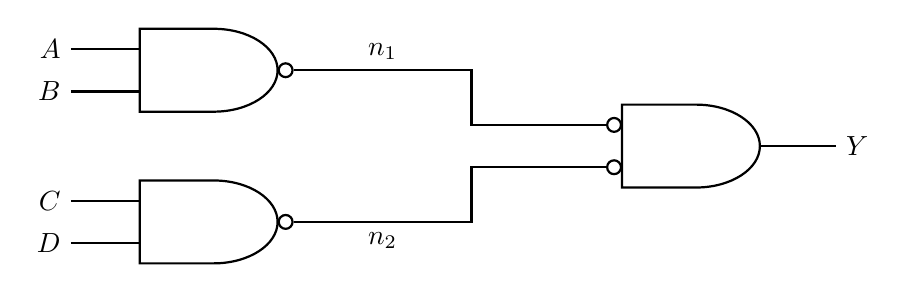
\begin{tikzpicture}[x=1.25cm,y=1.12cm,thick,
      inversion/.style={draw,circle,inner sep=0pt,minimum size=5pt}]
    \foreach \level/\first/\second/\branch in {0.86/A/B/upper,-0.86/C/D/lower} {
      \draw (1.18,{\level-0.47}) -- (1.18,{\level+0.47})
        -- (1.93,{\level+0.47})
        arc[start angle=90,end angle=-90,x radius=0.65,y radius=0.47]
        -- cycle;
      \draw (0.48,{\level+0.24}) node[left] {\(\first\)} -- (1.18,{\level+0.24})
        (0.48,{\level-0.24}) node[left] {\(\second\)} -- (1.18,{\level-0.24});
      \node[inversion,anchor=west] (\branch) at (2.58,\level) {};
    }
    \draw (6.08,-0.47) -- (6.08,0.47) -- (6.83,0.47)
      arc[start angle=90,end angle=-90,x radius=0.65,y radius=0.47]
      -- cycle;
    \node[inversion,anchor=east] (invertUpper) at (6.08,0.24) {};
    \node[inversion,anchor=east] (invertLower) at (6.08,-0.24) {};
    \draw (upper.east) -- (4.55,0.86) node[midway,above] {\(n_1\)}
      |- (invertUpper.west);
    \draw (lower.east) -- (4.55,-0.86) node[midway,below] {\(n_2\)}
      |- (invertLower.west);
    \draw (7.48,0) -- (8.25,0) node[right] {\(Y\)};
  \end{tikzpicture}
  \end{latin}
  \caption{مدار مثال اسلاید ۱۶ با گره‌های میانی \(n_1\) و \(n_2\).
    حباب روی هر پایه مقدار منطقی آن پایه را وارونه می‌کند.
    بازترسیم از اسلاید ۱۶ \cite{powerslides}.}
  \label{fig:power-slide-and-activity}
\end{figure}

دو گیت سمت چپ در خروجی حباب دارند، پس \lr{NAND} هستند.
گیت سمت راست به‌دلیل حباب‌های ورودی، ابتدا هر دو ورودی را
وارونه می‌کند و سپس \lr{AND} می‌گیرد. بنابراین \(Y\) تنها
هنگامی یک می‌شود که \(n_1\) و \(n_2\) هر دو صفر باشند.
این وضعیت دقیقاً زمانی رخ می‌دهد که هر چهار ورودی اولیه یک باشند
\cite[مثال ۵.۲ و شکل \secnum{۵.۹}، صفحات ۱۸۷ و ۱۸۸]{weste}.

فرض می‌کنیم چهار ورودی در هر دوره مستقل و هم‌احتمال‌اند،
بردار ورودی بین دوره‌های متوالی مستقل است و گره‌ها میان
نمونه‌ها گذار اضافی ندارند. پس برای هر ورودی \(p=1/2\)
و \(\alpha=(1/2)(1/2)=1/4\) است. گره \(n_1\) فقط با یک بودن
هم‌زمان \(A\) و \(B\) صفر می‌شود. احتمال آن حالت
\((1/2)(1/2)=1/4\) است. برای \(n_2\)، زوج \(C,D\) همین نقش را
دارد. پس احتمال یک بودن و فعالیت هر گره میانی چنین است.
\[
  p_{n_1}=p_{n_2}=1-\frac14=\frac34,\qquad
  \alpha_{n_1}=\alpha_{n_2}=\frac14\times\frac34=\frac{3}{16}.
\]
دو گره میانی از دو زوج مستقل ورودی ساخته شده‌اند. بنابراین برای
احتمال صفر بودن هم‌زمان آن‌ها، دو احتمال \(1/4\) را در هم ضرب
می‌کنیم. نتیجه با شمارش چهار ورودی هم به دست می‌آید. تنها ترکیب
\((1,1,1,1)\) از میان ۱۶ ترکیب هم‌احتمال، \(Y=1\) می‌دهد.
با اعمال رابطه \eqref{eq:power-activity-independent} بر خروجی داریم.
\[
  p_Y=\frac14\times\frac14=\frac{1}{16},\qquad
  \alpha_Y=\frac{15}{16}\times\frac{1}{16}=\frac{15}{256}.
\]
اگر گره \(n_1\) را وارونه کنیم، احتمال یک بودن از \(3/4\) به
\(1/4\) می‌رسد. در محاسبه فعالیت فقط جای دو عامل
\(p\) و \(1-p\) عوض می‌شود و حاصل همان \(3/16\) است.

% !TeX root = ../complete.tex
\section{کاهش \lr{Switching Power}}
\label{sec:power-dynamic-reduction}

از رابطه \eqref{eq:power-switching} چهار کمیت برای کاهش توان به دست
می‌آیند. توان با \(\alpha\)، \(C_L\) و \(f\) متناسب است و با
مربع \(V_{DD}\) تغییر می‌کند. شرط این مقایسه آن است که هنگام تغییر
هر کمیت، بقیه ثابت باشند. در طراحی واقعی، تغییر ظرفیت یا ولتاژ می‌تواند
تأخیر مسیر را نیز تغییر دهد. پس بعد از برآورد توان، باید معتبر بودن
فرض‌ها و برقراری محدودیت زمانی را بررسی کرد
\cite[بخش \secnum{۵.۲}، صفحات ۱۸۵ تا ۱۹۳]{weste}
\cite[اسلایدهای ۱۳ و ۱۷ تا ۱۹]{powerslides}.

\subsection{توقف ساعت یک بلوک بی‌کار}
\label{sec:power-clock-gating}

\lr{Register} یک یا چند بیت را نگه می‌دارد. در این مثال، در هر لبه
صعودی ساعت، داده ورودی را می‌گیرد و تا لبه بعد نگه می‌دارد. اگر
\lr{Register} ورودی یک بلوک در چند چرخه به‌روزرسانی لازم نداشته باشد،
با \lr{Clock Gating} می‌توان لبه‌های ساعتِ همان بلوک را در آن مدت
متوقف کرد. در این حالت هم گذارهای شاخه ساعت و هم گذارهایی که از
تغییر خروجی این \lr{Register} ناشی می‌شوند، کاهش می‌یابند. اگر
ورودی‌های دیگری مستقل از آن \lr{Register} تغییر کنند، ممکن است بخشی
از منطق بلوک همچنان گذار داشته باشد
\cite[بخش \secnum{۵.۲.۱.۱}، صفحه ۱۸۶]{weste}
\cite[اسلاید ۱۷]{powerslides}.

برای فهم مدار، ساعت اصلی را \(\mathrm{clk}\)، سیگنال اجازه عبور را
\(e\) و ساعت بلوک را \(\mathrm{gclk}\) بنامید. در مدل منطقی،
\(\mathrm{gclk}=\mathrm{clk}\land e\) است. وقتی \(e=1\)، ساعت
بلوک از ساعت اصلی پیروی می‌کند و وقتی \(e=0\)، ساعت بلوک صفر
می‌ماند. اگر \(e\) در میانه سطح بالای ساعت تغییر کند، این گیت
می‌تواند پالس را کوتاه کند یا لبه‌ای ناخواسته به \lr{Register}
بفرستد. راه شکل \secnum{۵.۷} کتاب استفاده از \lr{Latch} است،
یعنی عنصر حافظه‌ای که وقتی ساعت صفر است مقدار اجازه عبور را می‌پذیرد
و در تمام زمان یک‌بودن ساعت آن را ثابت نگه می‌دارد
\cite[شکل \secnum{۵.۷}، صفحه ۱۸۶]{weste}.

اگر یک شاخه در ۱۰ دوره کامل ساعت اصلی تنها چهار دوره پالس داشته
باشد، \(\alpha\) آن شاخه نسبت به ساعت اصلی \(4/10=0.4\) است.
با ثابت بودن ولتاژ و ظرفیت شاخه، توان سوئیچینگ این شاخه ۴۰ درصد
حالت بدون \lr{Clock Gating} می‌شود. اندازه‌گیری صرفه‌جویی کل بلوک
به فعالیت داده‌ها، مصرف مدار کنترل و اجزایی که همچنان ساعت می‌گیرند
نیز وابسته است. تغذیه مدار در این روش وصل می‌ماند.

\subsection{کاهش ظرفیت و کنترل تأخیر}
\label{sec:power-capacitance-reduction}

کوتاه کردن سیمِ گره‌هایی که زیاد سوئیچ می‌کنند، سهم ظرفیت سیم را در
رابطه \eqref{eq:power-node-sum} کم می‌کند. کوچک کردن یک گیت، ظرفیت
ورودی آن را برای مرحله پیشین و ظرفیت \lr{Diffusion} خود گیت را نیز
کم می‌کند. در عوض، گیت کوچک‌تر معمولاً همان بار بعدی را کندتر شارژ
می‌کند. در یک مسیر، اثر هر تغییر را روی ظرفیت، تأخیر مراحل پیش و پس
از گیت و فعالیت گره‌ها بررسی می‌کنیم. مبنای بررسی تأخیر همان
\NotesTopic{sec:delay-path-model}{مدل مسیر در \lr{Logical Effort}}
است \cite[بخش \secnum{۵.۲.۲}، صفحات ۱۸۸ تا ۱۹۰]{weste}
\cite[اسلاید ۱۸]{powerslides}.

برای یک سیم بلند، یکی از گزینه‌ها این است که یک
\lr{Inverter} یا \lr{Buffer} در ابتدای سیم قرار دهیم تا
ظرفیت بزرگ سیم مستقیماً به خروجی گیت منطقی تحمیل نشود. در این
آرایش، گیت منطقی ورودی مرحله جدید را راه‌اندازی می‌کند و
مرحله جدید سیم را شارژ و تخلیه می‌کند. با افزایش اندازه
\lr{Buffer}، بار ورودی آن نیز بیشتر می‌شود. برای تصمیم‌گیری،
ظرفیت ورودی و ظرفیت‌های درونی مرحله اضافه، قطبیت خروجی و تأخیر
کل مسیر را در کنار ظرفیت سیم در نظر می‌گیریم
\cite[بخش \secnum{۵.۲.۲}، صفحه ۱۸۸]{weste}
\cite[اسلاید ۱۸]{powerslides}.

برای نمونه، دو \lr{Inverter} پیاپی با ظرفیت‌های ورودی ۱ و ۴ واحد
و بار نهایی ۱۶ واحد در نظر بگیرید. واحد ظرفیت را ظرفیت ورودی
\lr{Inverter} مرجع و \(\tau\) را واحد تأخیر فصل قبل می‌گیریم.
در مدل عادی‌شده فصل تأخیر، تأخیر هر \lr{Inverter} شامل یک واحد
سهم درونی و نسبت ظرفیت بار به ظرفیت ورودی آن است. با چشم‌پوشی از
ظرفیت سیم و شاخه‌های فرعی، فقط دو گیت داریم. اگر ظرفیت ورودی گیت
دوم را به ۲ واحد برسانیم، تأخیر کل به‌ترتیب قبل و بعد از تغییر چنین است.
\[
  \begin{aligned}
    D_{\mathrm{before}} &= \left(1+\frac{4}{1}\right)
                         +\left(1+\frac{16}{4}\right)=10,\\
    D_{\mathrm{after}}  &= \left(1+\frac{2}{1}\right)
                         +\left(1+\frac{16}{2}\right)=12.
  \end{aligned}
\]
برای تبدیل این اعداد به تأخیر، هرکدام را در \(\tau\) ضرب می‌کنیم.
تأخیر نرمال‌شده گیت اول از ۵ به ۳ کم شده، اما
تأخیر گیت دوم از ۵ به ۹ رسیده است. گیت کوچک‌تر ظرفیت ورودی کم‌تری
دارد و با فرض فعالیت و دامنه یکسان، انرژی شارژ مربوط به همین بخش
از بار گره میانی نصف می‌شود. اگر مهلت مسیر کم‌تر از \(12\tau\)
باشد، این انتخاب با وجود کاهش انرژیِ بار میانی پذیرفتنی نیست.

\subsection{تنظیم ولتاژ و فرکانس}
\label{sec:power-voltage-frequency}

برای مقایسه دو حالت کاریِ یک گره، \(V_1,f_1\) و \(V_2,f_2\)
را ولتاژ و فرکانس حالت‌های اول و دوم بگیرید. اگر ظرفیت و فعالیت
به‌ازای هر دوره ثابت باشند و توان سوئیچینگ حالت اول مثبت باشد، با
تقسیم رابطه \eqref{eq:power-switching} برای دو حالت، عامل‌های مشترک
ساده می‌شوند و نسبت زیر به دست می‌آید.
\begin{equation}
  \frac{P_{\mathrm{sw},2}}{P_{\mathrm{sw},1}}
    =\left(\frac{V_2}{V_1}\right)^2\frac{f_2}{f_1}.
  \label{eq:power-voltage-frequency-ratio}
\end{equation}
مثلاً اگر ولتاژ به ۸۰ درصد و فرکانس به نصف مقدار اولیه برسد، نسبت
توان \(0.8^2\times0.5=0.32\) می‌شود. برای یک کار با تعداد دوره
ثابت، نصف شدن فرکانس زمان انجام کار را دو برابر می‌کند. در این مثال
نسبت انرژی سوئیچینگِ آن کار \(0.32\times2=0.64\) است. اگر ولتاژ
ثابت بماند، کاهش فرکانس به‌تنهایی توان سوئیچینگ را کم می‌کند، ولی
با همین فرض‌ها انرژی سوئیچینگِ کار ثابت می‌ماند. نتیجه به مؤلفه
سوئیچینگ محدود است و انرژی نشتی در زمان اجرای طولانی‌تر می‌تواند
تغییر کند \cite[بخش‌های \secnum{۵.۲.۳} و \secnum{۵.۲.۴}،
صفحات ۱۹۰ تا ۱۹۳]{weste}.

ولتاژ کم‌تر معمولاً جریان راه‌اندازی را کم و گذار را کندتر می‌کند.
ساعت را باید چنان انتخاب کرد که مدار با این تأخیر هنوز کار را در
زمان مقرر انجام دهد. در \lr{Dynamic Voltage and Frequency Scaling}
یا \lr{DVFS}، این دو کمیت برحسب نیاز عملکردیِ بار کاری تنظیم
می‌شوند. در طراحی با \lr{Voltage Domain}، هر بلوک می‌تواند تغذیه
مختص خود را داشته باشد. وقتی سیگنالی از تغذیه کم‌تر به بیش‌تر می‌رود،
سطح یکِ فرستنده ممکن است برای خاموش‌کردن کامل \lr{pMOS} گیرنده
کافی نباشد. \lr{Level Converter} دامنه سیگنال را برای بلوک گیرنده
بازسازی می‌کند. زمان و انرژی خود مبدل نیز در مقایسه معماری‌ها سهم
دارند \cite[بخش \secnum{۵.۲.۳}، صفحات ۱۹۰ تا ۱۹۲]{weste}
\cite[اسلاید ۱۹]{powerslides}.

در \lr{Resonant Clock}، کتاب راه دیگری را برای بار دوره‌ای معرفی
می‌کند. انرژی میان خازن و سلف، یعنی عنصری که انرژی را در میدان
مغناطیسی ذخیره می‌کند، مبادله می‌شود. راه‌انداز در هر دوره انرژی
ازدست‌رفته در مقاومت‌ها را جبران می‌کند. این تغییر مسیر انرژی، فرض
مدل معمول شارژ از منبع و تخلیه کامل به زمین را عوض می‌کند. در برابر
امکان کاهش مصرف، مدار به اجزای بیشتر و فرکانس کاری متناسب با
شبکه تشدید نیاز دارد \cite[بخش \secnum{۵.۲.۶}، صفحه ۱۹۳]{weste}.

% !TeX root = ../complete.tex
\section{مسیرهای جریان و برآورد \lr{Static Power}}
\label{sec:power-static}

\subsection{مصرف توان در یک وضعیت منطقی ثابت}
\label{sec:power-static-sources}

در مدل \lr{Switch} یک گیت مکمل \lr{CMOS}، پس از پایان گذار، یکی
از شبکه‌های \lr{Pull-up} یا \lr{Pull-down} خاموش است و مسیر مستقیم
روشنی میان تغذیه و زمین وجود ندارد. خازن خروجی نیز پس از رسیدن به
ولتاژ نهایی جریان شارژ نمی‌گیرد. در ترانزیستور واقعی، حتی در این وضعیت
جریان‌های کوچک از چند مسیر عبور می‌کنند. برای تغذیه ثابت، اگر این
جریان‌ها سهم‌های جداگانه‌ی جریان کشیده‌شده از همان تغذیه باشند، برآورد
توان ساکن از رابطه زیر به دست می‌آید
\cite[رابطه \secnum{۵.۱۲} و بخش \secnum{۵.۳.۱}،
صفحات ۱۸۵ و ۱۹۴ تا ۱۹۷]{weste}\cite[اسلایدهای ۱۰ و ۲۰]{powerslides}.
\begin{equation}
  P_{\mathrm{stat}}
    =V_{DD}\bigl(I_{\mathrm{sub}}+I_{\mathrm{gate}}+
                 I_{\mathrm{junct}}+I_{\mathrm{cont}}
           \bigr).
  \label{eq:power-static}
\end{equation}
هر جمله داخل پرانتز جریان است و ضرب جمع جریان‌ها در ولتاژ، توان
را برحسب وات می‌دهد. مسیرهای فیزیکی نشتی در
\NotesTopic{sec:leakage}{فصل مدل ترانزیستور} بررسی شده‌اند. در اینجا
اثر هر مسیر را بر جریان کشیده‌شده از منبع دنبال می‌کنیم.

\begin{itemize}
  \item \(I_{\mathrm{sub}}\) سهم \lr{Subthreshold Leakage} است.
    زیر آستانه، ترانزیستور خاموش هنوز می‌تواند جریان کوچکی از مسیر
    کانال عبور دهد. ولتاژهای پایانه‌ها و دما بر این جریان اثر دارند.
    در چند ترانزیستور خاموشِ سری، ولتاژ گره میانی از تعادل جریان
    به دست می‌آید و بایاس هر ترانزیستور با حالت تک‌ترانزیستور فرق
    می‌کند. کاهش نشتی حاصل در بسیاری از وضعیت‌های ورودی را
    \lr{Stack Effect} می‌نامیم.
  \item \(I_{\mathrm{gate}}\) سهم \lr{Gate Leakage} است. اختلاف
    پتانسیل در دو سوی دی‌الکتریک نازک گیت می‌تواند موجب عبور حامل‌ها
    به‌واسطه‌ی \lr{Tunneling} شود. ضخامت و جنس دی‌الکتریک و ولتاژ
    دو سوی آن تعیین می‌کنند این سهم چقدر باشد.
  \item \(I_{\mathrm{junct}}\) سهم \lr{Junction Leakage} است.
    ناحیه‌های \lr{Source} و \lr{Drain} با \lr{Body} پیوند تشکیل
    می‌دهند. حتی یک پیوند با بایاس معکوس جریان کوچکی دارد. میدان
    زیاد نزدیک پیوند می‌تواند سهم سازوکارهایی مانند
    \lr{Band-to-Band Tunneling} را بیشتر کند.
  \item \(I_{\mathrm{cont}}\) سهم \lr{Contention Current} است.
    برای نمونه، در \lr{Pseudo-nMOS} یک \lr{pMOS} همیشه روشن
    خروجی را به سمت تغذیه می‌کشد. هنگامی که شبکه \lr{nMOS} خروجی
    را پایین نگه می‌دارد، هر دو مسیر هم‌زمان هدایت می‌کنند و جریان
    ماندگار برقرار است. این جریان در مدل ماندگار گیت مکمل
    \lr{CMOS} وجود ندارد. \lr{Short-Circuit Current} بخش
    \ref{sec:power-short-circuit} پالس جریان در زمان گذار است.
\end{itemize}

\subsection{برآورد نشتی از عرض افزاره‌ها}
\label{sec:power-static-estimate}

وقتی مقدار یک نشتی به‌ازای واحد عرض معلوم باشد، نخست ترانزیستورها
را برحسب نوع و وضعیت بایاس گروه‌بندی می‌کنیم. در هر گروه، تعداد
افزاره‌ها ضرب‌در عرض متوسط، عرض کل گروه را می‌دهد. اگر کسری از
عرض کل در وضعیت دارای نشتی موردنظر باشد، همان کسر را در عرض کل
و جریان بر واحد عرض ضرب می‌کنیم. برای مثال، در مدل ساده‌ی نشتی
زیرآستانه، \(W_g\) عرض کل گروه \(g\)، \(b_g\) کسر عرضِ خاموش
و \(j_{\mathrm{off},g}\) جریان خاموش بر واحد عرض آن گروه است.
\cite[بخش \secnum{۵.۳.۱.۵}، صفحه ۱۹۷]{weste}
\begin{equation}
  I_{\mathrm{sub}}\approx\sum_g b_g W_g j_{\mathrm{off},g}.
  \label{eq:power-width-leakage}
\end{equation}
\(b_g\) بی‌بعد است. اگر \(W_g\) برحسب میکرومتر و
\(j_{\mathrm{off},g}\) برحسب نانوآمپر بر میکرومتر باشد، حاصل ضرب
برحسب نانوآمپر خواهد بود. ثبات مقدار جریان بر واحد عرض در هر گروه
یک تقریب است. به‌ویژه، جدول \secnum{۵.۲} کتاب نشان می‌دهد که در
یک \lr{NAND} سه‌ورودی، تغییر ترتیب ورودی‌ها می‌تواند ولتاژ گره‌های
میانی و درنتیجه نشتی را عوض کند \cite[صفحه ۱۹۶]{weste}.

در مثال ۵.۴ کتاب و اسلایدهای ۲۱ و ۲۲، دوباره همان تراشه‌ی بخش
\ref{sec:power-effective-capacitance} را بررسی می‌کنیم. از ۵۰ میلیون
ترانزیستور منطق با عرض متوسط \qty{0.30}{\micro\metre}، سهم
۵ درصد در گروه با آستانه پایین‌تر و ۹۵ درصد در گروه آستانه بالا
قرار می‌گیرند. اسلاید گروه ۵ درصدی را \lr{Normal \(V_t\)} و
کتاب در مثال ۵.۴ آن را \lr{low-threshold} می‌نامد. هر دو منبع
برای این گروه در حالت خاموش، مقدار
\qty[per-mode=symbol]{100}{\nano\ampere\per\micro\metre}
به کار می‌برند. \(W_{\mathrm{nom}}\) عرض کل این گروه و
\(W_{\mathrm{high}}\) عرض کل گروه آستانه بالاست.
همه‌ی ۹۵۰ میلیون ترانزیستور حافظه با عرض متوسط
\qty{0.10}{\micro\metre} در گروه آستانه بالا قرار می‌گیرند.
عرض کل دو گروه از جمع عرض ترانزیستورهایشان به دست می‌آید
\cite[مثال ۵.۴، صفحه ۱۹۷]{weste}\cite[اسلایدهای ۲۱ و ۲۲]{powerslides}.
\[
  \begin{aligned}
    W_{\mathrm{nom}}&=(50\times10^6)(0.05)
                       (\qty{0.30}{\micro\metre})
                     =\qty{0.75e6}{\micro\metre},\\
    W_{\mathrm{high}}&=(50\times10^6)(0.95)
                        (\qty{0.30}{\micro\metre})
                        +(950\times10^6)(\qty{0.10}{\micro\metre})\\
                    &=\qty{109.25e6}{\micro\metre}.
  \end{aligned}
\]
در این برآورد، نصف عرض هر گروه در حالت خاموش است. \lr{Stack Effect}
را کنار می‌گذاریم و با مقادیر خاموشِ داده‌شده در مثال، سهم کانال را
حساب می‌کنیم. برای سهم گیت فرض می‌کنیم نیمه‌ی روشنِ عرض کل دارای
آن نشتی است. پس نصف مجموع عرض را در
\qty[per-mode=symbol]{5}{\nano\ampere\per\micro\metre} ضرب می‌کنیم.
\[
  \begin{aligned}
    I_{\mathrm{sub}} &\approx \tfrac12\bigl[
       W_{\mathrm{nom}}(\qty[per-mode=symbol]{100}{\nano\ampere\per\micro\metre})
      +W_{\mathrm{high}}(\qty[per-mode=symbol]{10}{\nano\ampere\per\micro\metre})
      \bigr]\approx\qty{584}{\milli\ampere},\\
    I_{\mathrm{gate}}&\approx\tfrac12(W_{\mathrm{nom}}+W_{\mathrm{high}})
        (\qty[per-mode=symbol]{5}{\nano\ampere\per\micro\metre})
        =\qty{275}{\milli\ampere}.
  \end{aligned}
\]
با فرض ناچیز بودن نشتی پیوند و نبود مسیر ماندگار ناشی از هدایت
هم‌زمان، جمع این دو جریان در تغذیه \qty{1.0}{\volt} حدود
\qty{859}{\milli\watt} توان ساکن می‌دهد. این مقدار در همان مدل
تراشه حتی اگر ساعت متوقف شود و وضعیت بایاس و دما ثابت بمانند،
با صفر شدن توان سوئیچینگ از بین نمی‌رود. نسبت آن به برآورد
\qty{6.1}{\watt} سوئیچینگ بخش \ref{sec:power-effective-capacitance}
حدود ۱۴ درصد است. هر دو برآورد به داده‌ها و فرض‌های همین مثال
وابسته‌اند.

\subsection{کاهش نشتی با انتخاب افزاره و وضعیت ورودی}
\label{sec:power-leakage-controls}

مقدار \(V_t\) تعیین می‌کند ترانزیستور در یک ولتاژ گیت معین چه
مقدار جریان عبور می‌دهد. با ثابت بودن سایر بایاس‌ها و دما، بالا بردن
آستانه به اندازه \(\Delta V_t\) جمله نماییِ جریان زیرآستانه را
در مدل فصل ۲ در عامل زیر ضرب می‌کند. \(S\) تغییر ولتاژ لازم برای
یک دهه تغییر جریان است
\cite[بخش‌های \secnum{۲.۴.۴} و \secnum{۵.۳.۱.۱}]{weste}.
\[
  \frac{I_{\mathrm{sub,new}}}{I_{\mathrm{sub,old}}}
  \approx 10^{-\Delta V_t/S}.
\]
برای مثال، اگر \(S\) برابر \qty{100}{\milli\volt} بر دهه باشد،
افزایش \qty{50}{\milli\volt} آستانه، نمای کسر را به \(-1/2\)
می‌رساند. \(10^{-1/2}=1/\sqrt{10}\) است، پس جریان تخمینی به حدود
۳۲ درصد مقدار اولیه می‌رسد. مقدار \(S\) و جریان اولیه از بایاس، دما
و فناوری می‌آیند.

در کتابخانه دارای چند آستانه، \lr{High-\(V_t\)} برای مسیر دارای
مهلت کافی، نشتی زیرآستانه‌ی کمتری دارد. \lr{Low-\(V_t\)} در بخش
حساس به تأخیر می‌تواند جریان روشن بیشتری بدهد. دی‌الکتریک ضخیم‌تر
در فناوری‌هایی که آن گزینه را دارند، می‌تواند نشتی گیت را کم کند.
سرعت و سازگاری سلول با ولتاژ کاری هنگام انتخاب هر نوع بررسی می‌شوند
\cite[بخش \secnum{۵.۳.۳}، صفحه ۱۹۹]{weste}.

در \lr{Body Bias}، ولتاژ \lr{Body} نسبت به \lr{Source} تنظیم
می‌شود. در \lr{nMOS}، افزایش بایاس معکوس پیوند بدنه و سورس در
محدوده معتبر مدل، آستانه را بالا می‌برد و می‌تواند جریان زیرآستانه
را کم کند. بایاس معکوس زیاد، میدان پیوند را افزایش می‌دهد و ممکن
است نشتی پیوند بیشتر شود. با \lr{Input Vector Control} نیز می‌توان
هنگام بی‌کاری ترکیبی از ورودی‌ها را اعمال کرد که وضعیت ترانزیستورهای
خاموش در شاخه‌های سری نشتی کمتری ایجاد کند. هزینه تغییر ورودی‌ها
و صرفه‌جویی در طول بی‌کاری هر دو در ارزیابی این روش سهم دارند
\cite[بخش‌های \secnum{۵.۳.۴} و \secnum{۵.۳.۵}،
صفحات ۱۹۹ و ۲۰۰]{weste}.

% !TeX root = ../complete.tex
\section{قطع تغذیه بلوک با \lr{Power Gating}}
\label{sec:power-gating}

\subsection{مسیر تغذیه، جداسازی خروجی و حفظ وضعیت}
\label{sec:power-gating-operation}

در \NotesTopic{sec:power-clock-gating}{\lr{Clock Gating}}، ساعت
بلوک متوقف می‌شود و ریل تغذیه به مدار وصل می‌ماند. در \lr{Power Gating}،
یک ترانزیستور سری، مسیر تغذیه بلوک را در حالت خواب قطع می‌کند.
در شکل \ref{fig:power-gating-header}، یک \lr{pMOS Header} میان
تغذیه اصلی \(V_{DD}\) و ریل تغذیه بلوک قرار دارد. ولتاژ ریل بعد
از کلید را \(V_{DDV}\) می‌نامیم. آن را ریل تغذیه مجازی می‌گویند،
زیرا مقدارش به وضعیت کلید، بار و نشتی بلوک وابسته است. گزینه‌ی دیگر
\lr{nMOS Footer} است که به‌جای تغذیه بالا، مسیر اتصال به زمین را
قطع می‌کند \cite[بخش \secnum{۵.۳.۲}، صفحات ۱۹۷ و ۱۹۸]{weste}
\cite[اسلاید ۲۳]{powerslides}.

\begin{figure}[htbp]
  \centering
  \begin{latin}
  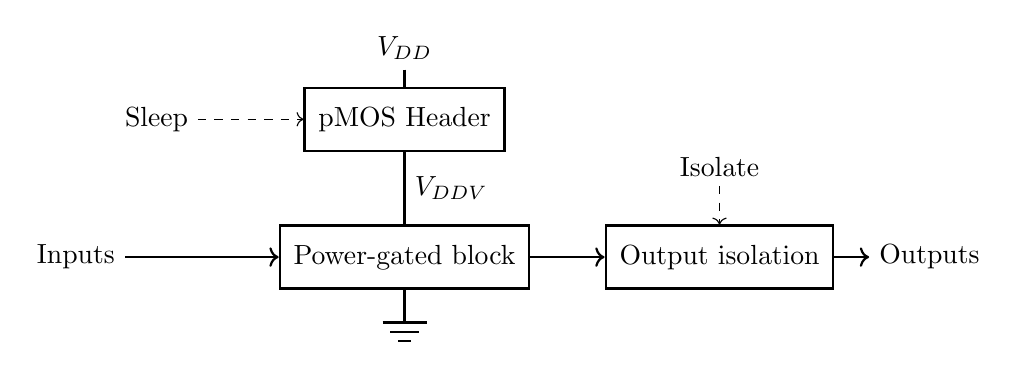
\begin{tikzpicture}[
    x=1cm,y=1cm,
    component/.style={draw,thick,minimum height=8mm,align=center,inner sep=5pt}
  ]
    \node[component] (header) at (0,1.75) {pMOS Header};
    \node[component] (block) at (0,0) {Power-gated block};
    \node[component] (isolate) at (4,0) {Output isolation};
    \node (supply) at (0,2.65) {\(V_{DD}\)};
    \node (sleep) at (-3.15,1.75) {Sleep};
    \node (clamp) at (4,1.15) {Isolate};
    \draw[thick] (supply) -- (header.north);
    \draw[thick] (header.south) -- (block.north)
      node[midway,right] {\(V_{DDV}\)};
    \draw[dashed,->] (sleep.east) -- (header.west);
    \draw[dashed,->] (clamp.south) -- (isolate.north);
    \draw[->,thick] (-3.55,0) node[left] {Inputs} -- (block.west);
    \draw[->,thick] (block.east) -- (isolate.west);
    \draw[->,thick] (isolate.east) -- (5.9,0) node[right] {Outputs};
    \draw[thick] (block.south) -- (0,-0.83);
    \draw[thick] (-0.28,-0.83) -- (0.28,-0.83);
    \draw[thick] (-0.18,-0.95) -- (0.18,-0.95);
    \draw[thick] (-0.08,-1.07) -- (0.08,-1.07);
  \end{tikzpicture}
  \end{latin}
  \caption{مسیر تغذیه و مسیر داده در یک بلوک دارای \lr{Power Gating}.
    \lr{Sleep} کلید تغذیه را کنترل می‌کند و \lr{Isolate} سطح خروجی را
    هنگام قطع تغذیه معتبر نگه می‌دارد. طرح مفهومی از شکل \secnum{۵.۲۴}
    کتاب و اسلاید ۲۳ اقتباس شده است \cite{weste,powerslides}.}
  \label{fig:power-gating-header}
\end{figure}

در حالت فعال، کلید روشن است و ریل مجازی نزدیک \(V_{DD}\) می‌ماند.
در خواب، کلید خاموش می‌شود و بار ذخیره‌شده روی ریل مجازی می‌تواند
از مسیرهای نشتی کاهش یابد. تا زمانی که تغذیه بلوک دوباره برقرار شود،
خروجی آن ممکن است در محدوده نامعتبر بین صفر و یک بماند. مدار
\lr{Output Isolation} با تغذیه برقرار، پیش از قطع تغذیه خروجی را
به یک سطح مشخص مانند صفر محدود می‌کند. اگر بلوک باید پس از بیداری
از همان داده ادامه دهد، داده را در \lr{Retention Register} با تغذیه
برقرار یا در حافظه‌ای بیرون از دامنه‌ی خاموش نگه می‌دارند. پس از
وصل تغذیه، ریل فرصت بازیابی دارد و وضعیت لازم بازیابی یا مقداردهی
اولیه می‌شود. جداسازی هنگامی برداشته می‌شود که خروجی‌های بلوک معتبر
باشند \cite[بخش \secnum{۵.۳.۲}، صفحات ۱۹۷ تا ۱۹۹]{weste}.

\subsection{افت روی کلید و اثر آن بر تأخیر}
\label{sec:power-header-delay}

در یک برآورد دست‌اول برای کلید روشن، \(W\) عرض مؤثر کلید،
\(R_h\) مقاومت روشن و \(r_w\) حاصل‌ضرب مقاومت روشن در عرض است.
\(r_w\) برای طول کانال و شرایط بایاس مشخص داده می‌شود و می‌توان آن
را با اهم‌میکرومتر بیان کرد. اگر جریان نماینده‌ی بلوک در حالت فعال
\(I_{\mathrm{on}}\) باشد، قانون اهم افت ریل را به عرض کلید ربط می‌دهد.
\begin{equation}
  R_h\approx\frac{r_w}{W},\qquad
  \Delta V=V_{DD}-V_{DDV}\approx I_{\mathrm{on}}R_h.
  \label{eq:power-header-droop}
\end{equation}
ضرب آمپر در اهم واحد ولت دارد. بزرگ‌تر کردن عرض، در این مدل
مقاومت و افت را کاهش می‌دهد. به‌کارگیری جریان متوسط برای بلوک بزرگ
هنگامی مناسب‌تر است که رویدادهای سوئیچینگ در زمان پخش شوند و ظرفیت
روی ریل مجازی، نوسان ولتاژ را هموار کند. اگر چند بار هم‌زمان جریان
زیادی بکشند، افت گذرا می‌تواند با برآورد متوسط تفاوت داشته باشد
\cite[بخش \secnum{۵.۳.۲.۱}، صفحات ۱۹۸ و ۱۹۹]{weste}.

برای مرتبط کردن افت ریل با تأخیر، \(V\) را ولتاژ مؤثر تغذیه بلوک،
\(V_t>0\) را آستانه‌ی مؤثر و \(D(V)\) را تأخیر مسیر در آن ولتاژ
می‌گیریم. برآورد فصل ۳ از تقسیم بار جابه‌جاشده بر جریان شروع می‌شود.
برای تغییر ولتاژ به اندازه‌ی کسری ثابت از \(V\)، بار با \(V\) متناسب
است. در \lr{Alpha-Power Law} جریان راه‌اندازی با \((V-V_t)^m\)
متناسب است. توان تجربی \(m\) معمولاً بین ۱ و ۲ است. کتاب آن را
\(\alpha\) می‌نویسد. در این فصل، \(\alpha\) برای \lr{Activity Factor}
به کار می‌رود. اگر ظرفیت و پارامترهای مدل ثابت باشند، برای \(V>V_t\)
با ثابت مثبت \(K\) داریم
\cite[رابطه \secnum{۴.۲۹}، صفحه ۱۶۲]{weste}.
\begin{equation}
  D(V)=K\frac{V}{(V-V_t)^m}.
  \label{eq:power-above-threshold-delay}
\end{equation}
\(K\) ظرفیت، ضرایب جریان و عوامل ثابت مربوط به مسیر را در بر می‌گیرد.
در این نوشتار، واحد آن \(\mathrm{s}\,\mathrm{V}^{m-1}\) است تا پس
از ضرب در \(V/(V-V_t)^m\)، حاصل واحد زمان داشته باشد. با تقسیم تأخیر ریل
مجازی بر تأخیر اولیه، \(K\) حذف می‌شود و نسبت زیر از مدل به دست می‌آید.
\begin{equation}
  \frac{D(V_{DD}-\Delta V)}{D(V_{DD})}
    =\left(1-\frac{\Delta V}{V_{DD}}\right)
      \left(\frac{V_{DD}-V_t}{V_{DD}-V_t-\Delta V}\right)^m.
  \label{eq:power-droop-delay-ratio}
\end{equation}
این نسبت برای \(0\leq\Delta V<V_{DD}-V_t\) تعریف شده است. اگر
افت صفر باشد، نسبت یک است. برای افت مثبت، عامل نخست کم‌تر از یک
و عامل دوم بزرگ‌تر از یک است. در این مدل با \(m\geq 1\)، کاهش
توانایی جریان‌دهی بر کاهش بار لازم برای گذار غلبه می‌کند.

برای افت کوچک می‌توان از حساسیت تأخیر استفاده کرد. اگر مقدار ولتاژ
از \(V\) به \(V-\Delta V\) برود، تقریب خطیِ تابع نزدیک \(V\)
می‌دهد \(D(V-\Delta V)-D(V)\approx-D'(V)\Delta V\).
برای محاسبه مشتق، \(D(V)=KV(V-V_t)^{-m}\) را به‌شکل ضرب دو
تابع می‌نویسیم. مشتق عامل اول \(K\) است. برای مشتق عامل دوم، قاعده
توان، \(-m(V-V_t)^{-m-1}\) را می‌دهد و طبق قاعده زنجیره‌ای آن را
در مشتق \(V-V_t\)، یعنی یک، ضرب می‌کنیم. حاصلِ قاعده ضرب پس از تقسیم بر
\(D(V)\)، دو جمله برای حساسیت باقی می‌گذارد. با \(V=V_{DD}\)
و \(\Delta D=D(V_{DD}-\Delta V)-D(V_{DD})\)، نتیجه چنین است.
\begin{equation}
  \frac{\Delta D}{D(V_{DD})}
  \approx\left(\frac{m}{V_{DD}-V_t}-\frac{1}{V_{DD}}\right)\Delta V.
  \label{eq:power-droop-delay-sensitivity}
\end{equation}
عبارت داخل پرانتز واحد معکوس ولت دارد و حاصل بی‌بعد است. هرچه
\(V_{DD}-V_t\) کوچک‌تر باشد، افت معین می‌تواند اثر نسبی بیشتری
بر تأخیر بگذارد. برای نمونه، با \(V_t/V_{DD}=0.30\) و \(m=1.4\)
عبارت داخل پرانتز \(1/V_{DD}\) است و در تقریب خطی درصد افزایش
تأخیر با درصد افت تغذیه برابر می‌شود. برابری درصدها به پارامترها
و کوچک بودن افت وابسته است.

\subsection{اندازه کلید و حداقل زمان خواب}
\label{sec:power-header-sizing}

اگر حد مجاز افت ریل \(\Delta V_{\max}>0\) معلوم باشد، با جای‌گذاری
\(R_h\) در رابطه \eqref{eq:power-header-droop} و اعمال شرط
\(\Delta V\leq\Delta V_{\max}\)، از مدل مقاومتی حد زیر بر عرض
به دست می‌آید. همه‌ی کمیت‌ها مثبت‌اند و ضرب و تقسیم جهت نامساوی
را تغییر نمی‌دهد.
\begin{equation}
  W\geq\frac{I_{\mathrm{on}}r_w}{\Delta V_{\max}}.
  \label{eq:power-header-width}
\end{equation}
در مثال ۵.۵ کتاب، تغذیه \qty{1}{\volt} و توان فعال میانگین حافظه
\qty{2}{\watt} است. تقسیم توان بر ولتاژ، جریان \qty{2}{\ampere}
را می‌دهد. کتاب برای بررسی افزایش تأخیرِ ۵ درصدی در همان مثال،
افت ریل را تقریباً ۵ درصدِ تغذیه می‌گیرد، یعنی
\qty{50}{\milli\volt}. مقاومت کلید از تقسیم این افت بر جریان
به‌دست می‌آید و حداکثر \qty{25}{\milli\ohm} است. برای
\(r_w=\qty{2}{\kilo\ohm\micro\metre}\) حد عرض چنین می‌شود
\cite[مثال ۵.۵، صفحات ۱۹۸ و ۱۹۹]{weste}.
\[
  W\geq\frac{\qty{2e3}{\ohm\micro\metre}}{\qty{25e-3}{\ohm}}
    =\qty{8e4}{\micro\metre}.
\]
واحد اهم ساده می‌شود و این عرض، مجموع عرض مؤثر کلیدهایی است که
می‌توان موازی بست. کتاب برای همان مثال از شبیه‌سازی مدار عرض کم‌تری
به دست می‌آورد و تفاوت را با تغییر مقاومت روشن در بایاس واقعی توضیح
می‌دهد. هنگام روشن شدن کلید، شارژ ریل مجازی می‌تواند جریان آغازین
بزرگی ایجاد کند. روشن کردن گروه‌های موازی در چند گام، روشی برای
محدود کردن این جریان آغازین است \cite[صفحه ۱۹۹]{weste}.

برای سنجش صرفه‌ی خواب، \(P_{\mathrm{idle}}\) را توان بلوک در حالت
بی‌کارِ دارای تغذیه، \(P_{\mathrm{sleep}}\) را توان بلوک در خواب و
\(E_{\mathrm{tr}}\) را انرژی اضافیِ ورود و خروج از خواب بگیرید.
اگر \(P_{\mathrm{idle}}>P_{\mathrm{sleep}}\)، در مدت خواب \(T_s\)
به‌اندازه‌ی \((P_{\mathrm{idle}}-P_{\mathrm{sleep}})T_s\) انرژی
صرفه‌جویی می‌شود. خواب هنگامی از لحاظ انرژی به‌صرفه است که این مقدار
از \(E_{\mathrm{tr}}\) بیشتر باشد. با حل نامساوی برای زمان، شرط
به صورت زیر است \cite[بخش \secnum{۵.۳.۲}، صفحات ۱۹۷ و ۱۹۸]{weste}.
\begin{equation}
  T_s > T_{\mathrm{BE}}
      =\frac{E_{\mathrm{tr}}}{P_{\mathrm{idle}}-P_{\mathrm{sleep}}}.
  \label{eq:power-gating-break-even}
\end{equation}
\(T_{\mathrm{BE}}\) زمان سربه‌سر انرژی است. ژول تقسیم بر وات
ثانیه می‌دهد. برای نمونه، اگر هزینه تغییر حالت \qty{1}{\nano\joule}
و کاهش توان \qty{2}{\milli\watt} باشد، تقسیم
\qty{1e-9}{\joule} بر \qty{2e-3}{\watt} برابر
\qty{0.5}{\micro\second} است. جدا از صرفه‌ی انرژی، زمان بیداری
نیز باید با مهلت پاسخ سامانه سازگار باشد.

% !TeX root = ../complete.tex
\section{مقایسه انرژی و تأخیر یک عملیات}
\label{sec:power-energy-delay}

\subsection{توان متوسط و انرژی به‌ازای هر عملیات}
\label{sec:power-energy-per-operation}

برای مقایسه دو پیاده‌سازی، ابتدا کاری را که هر دو باید انجام دهند
مشخص می‌کنیم. اگر مدار در بازه‌ای به مدت \(D\) فقط یک عملیات
انجام دهد و توان متوسط در همان مدت \(P_{\mathrm{avg}}\) باشد، از رابطه
\eqref{eq:power-interval}، انرژی عملیات \(E_{\mathrm{op}}=P_{\mathrm{avg}}D\)
به دست می‌آید. اگر توان را در بازه‌ای با چند عملیات اندازه بگیریم،
انرژی کل را بر تعداد عملیات کامل‌شده تقسیم می‌کنیم. با نرخ انجام
عملیات \(r_{\mathrm{op}}\)، یعنی تعداد عملیات کامل‌شده در ثانیه،
انرژی متوسط به‌ازای هر عملیات \(P_{\mathrm{avg}}/r_{\mathrm{op}}\)
است. در این کسر، واحد وات تقسیم بر معکوس ثانیه، ژول می‌دهد.
وقتی میانگین یک نتیجه در هر دوره ساعت باشد،
\(r_{\mathrm{op}}=f\) است. برای کاری که به چند دوره نیاز دارد،
رابطه را با نرخ واقعی انجام کار به کار می‌بریم
\cite[بخش‌های \secnum{۵.۴.۱} و \secnum{۵.۶}، صفحات
۲۰۰ و ۲۰۶]{weste}.

برای برآورد انرژی یک عملیات در تغذیه \(V\)، فرض کنید گره \(i\)
با ظرفیت معادل \(C_i\) در آن عملیات \(N_{\uparrow,i}\) بار از صفر
تا \(V\) شارژ می‌شود. مطابق رابطه \eqref{eq:power-source-energy}،
با جمع انرژی شارژِ همه گره‌ها، انرژی سوئیچینگ به دست می‌آید. مجموع
وزن‌دار \(C_{\mathrm{op}}=\sum_i N_{\uparrow,i} C_i\) واحد ظرفیت
دارد. اگر جریان نشتیِ متوسط \(I_{\mathrm{leak}}\) را برای مدت
انجام کار در نظر بگیریم و سهم پالس جریان مستقیم و هدایت هم‌زمان
ماندگار ناچیز باشند، مدل انرژی چنین است
\cite[رابطه \secnum{۵.۲۵}، صفحه ۲۰۲]{weste}.
\begin{equation}
  E_{\mathrm{op}}\approx E_{\mathrm{sw}}+E_{\mathrm{leak}}
    =C_{\mathrm{op}}V^2+I_{\mathrm{leak}}VD.
  \label{eq:power-operation-energy}
\end{equation}
جمله نخست با شمار شارژها و مربع ولتاژ تغییر می‌کند. در جمله دوم،
\(I_{\mathrm{leak}}V\) توان نشتی است و ضرب آن در مدت انجام کار،
انرژی نشتی را می‌دهد. بنابراین حتی کاهش توان نشتی می‌تواند با
بلندتر شدن زمان انجام کار به افزایش انرژی نشتی بینجامد.

\subsection{کمینه انرژی و کار در ولتاژ پایین}
\label{sec:power-minimum-energy}

در بخش \ref{sec:power-header-delay} از مدل جریان با اضافه‌ولتاژ
مثبت استفاده کردیم. اگر \(V\) پایین‌تر از \(V_t\) باشد، هنوز
جریان زیرآستانه وجود دارد. در تقریب بخش \secnum{۴.۴.۶.۴} کتاب،
جریان راه‌انداز با \(10^{V/S}\) متناسب است. \(S\) همان ولتاژ لازم
برای تغییر ده‌برابری جریان در مدل زیرآستانه است. با ثابت گرفتن
پارامترهای فناوری، ظرفیت مسیر و عوامل دیگری که بر جریان اثر دارند،
تقسیم بار متناسب با \(V\) بر جریان، تخمین زیر را برای مدت انجام
عملیاتِ محدود به یک مسیر می‌دهد
\cite[رابطه‌های \secnum{۴.۳۱} و \secnum{۵.۲۴}،
صفحات ۱۶۲ و ۲۰۲]{weste}.
\begin{equation}
  D(V)\approx K_s\,V\,10^{-V/S}.
  \label{eq:power-subthreshold-delay}
\end{equation}
\(K_s\) یک ضریب مثبت با واحد ثانیه بر ولت است که ظرفیت و ضریب
جریان مسیر را در بر می‌گیرد. اگر \(V\) به‌اندازه \(S\) کاهش
یابد، عامل نمایی ده برابر می‌شود. هم‌زمان، عامل خطی \(V\) کمی
کوچک‌تر می‌شود. در محدوده‌ای که اثر نمایی غالب است، تأخیر به‌سرعت
زیاد می‌شود. این مدل برای مقایسه نقطه‌های کاری معتبر در محدوده
زیرآستانه است. در ولتاژهای بسیار پایین، توانایی مدار در تولید و
حفظ سطوح منطقی نیز باید با معیار فصل ۲ بررسی شود.

برای نمونه، سه ولتاژ کاری زیر آستانه در یک مدل فرضی را مقایسه کنید.
می‌گیریم \(C_{\mathrm{op}}=\qty{20}{\femto\farad}\)،
\(I_{\mathrm{leak}}=\qty{5}{\nano\ampere}\) و
\(S=\qty{0.10}{\volt}\). برای این بازه فرض می‌کنیم تغییر
جریان نشتی با ولتاژ ناچیز است. زمان مرجع \(D_0=\qty{300}{\nano\second}\)
در \(V_0=\qty{0.30}{\volt}\) داده شده و همه‌ی ولتاژهای جدول در
محدوده معتبر مدل فرض می‌شوند. برای انتقال از زمان مرجع به زمان هر
ردیف، رابطه \eqref{eq:power-subthreshold-delay} را در دو ولتاژ بر
هم تقسیم می‌کنیم. حاصل به صورت زیر است.
\[
  \frac{D(V)}{D_0}\approx
    \frac{V}{V_0}\,10^{(V_0-V)/S}.
\]
در \qty{0.20}{\volt}، عامل نمایی ۱۰ و عامل خطی \(2/3\) است.
پس تأخیر تقریباً \((20/3)D_0=\qty{2000}{\nano\second}\) می‌شود.
در \qty{0.40}{\volt}، عامل نمایی \(1/10\) و عامل خطی \(4/3\)
است و تأخیر به \qty{40}{\nano\second} می‌رسد. برای نمونه در
ولتاژ پایین‌تر، جای‌گذاری در رابطه \eqref{eq:power-operation-energy}
دو مؤلفه را چنین می‌دهد.
\[
  \begin{aligned}
    E_{\mathrm{sw}}&=(\qty{20}{\femto\farad})(\qty{0.20}{\volt})^2
                     =\qty{0.80}{\femto\joule},\\
    E_{\mathrm{leak}}&=(\qty{5}{\nano\ampere})(\qty{0.20}{\volt})
                         (\qty{2.0}{\micro\second})
                     =\qty{2.0}{\femto\joule}.
  \end{aligned}
\]
همین محاسبه برای هر سه ولتاژ در جدول \ref{tab:power-energy-candidates}
آمده است. انرژی‌ها تا رقم اعشاری دوم نمایش داده شده‌اند تا جمع و
مقایسه ردیف‌ها روشن باشد.

\begin{table}[htbp]
  \centering
  \caption{انرژی و زمان یک عملیات در سه نقطه کاریِ یک مدل فرضی.
    \(E_{\mathrm{op}}\) از جمع انرژی سوئیچینگ و نشتی به دست آمده است.}
  \label{tab:power-energy-candidates}
  \begin{tabular}{ccccc}
    \toprule
    \(V\,(\unit{\volt})\) & \(D\,(\unit{\nano\second})\) &
    \(E_{\mathrm{sw}}\,(\unit{\femto\joule})\) &
    \(E_{\mathrm{leak}}\,(\unit{\femto\joule})\) &
    \(E_{\mathrm{op}}\,(\unit{\femto\joule})\) \\
    \midrule
    \num{0.20} & \num{2000} & \num{0.80} & \num{2.00} & \num{2.80} \\
    \num{0.30} & \num{300}  & \num{1.80} & \num{0.45} & \num{2.25} \\
    \num{0.40} & \num{40}   & \num{3.20} & \num{0.08} & \num{3.28} \\
    \bottomrule
  \end{tabular}
\end{table}

از میان این سه نقطه، \qty{0.30}{\volt} کم‌ترین انرژی را دارد.
در ولتاژ پایین‌تر، کاهش انرژی سوئیچینگ با افزایش انرژی نشتی در
زمان اجرای طولانی خنثی می‌شود. در ولتاژ بالاتر، انرژی سوئیچینگ
بزرگ‌تر است. این مقایسه کمینه را فقط در مجموعه سه گزینه مشخص
می‌کند. در مدار واقعی، تغییر فعالیت، آستانه یا دما می‌تواند
نقطه کمینه را جابه‌جا کند. این وابستگی در نقشه‌های شکل
\secnum{۵.۲۷} کتاب نیز دیده می‌شود \cite[صفحات ۲۰۲ و ۲۰۳]{weste}.

\subsection{کمینه \lr{Energy--Delay Product}}
\label{sec:power-edp}

گاهی هر دو هزینه انرژی عملیات و زمان اجرای آن در رتبه‌بندی اهمیت
دارند. معیار \lr{Energy--Delay Product} یا \lr{EDP}، حاصل‌ضرب
این دو با واحد ژول‌ثانیه است. محاسبه را برای \(V>V_t>0\) و با
\(C_{\mathrm{op}}>0\)، \(V_t\) و پارامترهای مسیر ثابت انجام می‌دهیم.
اگر انرژی سوئیچینگ غالب باشد، با ضرب انرژیِ رابطه
\eqref{eq:power-operation-energy} در تأخیرِ رابطه
\eqref{eq:power-above-threshold-delay} داریم
\cite[رابطه \secnum{۵.۲۶}، صفحه ۲۰۳]{weste}.
\begin{equation}
  \mathrm{EDP}(V)=E_{\mathrm{op}}(V)D(V)
       \approx K C_{\mathrm{op}}\frac{V^3}{(V-V_t)^m}.
  \label{eq:power-edp}
\end{equation}
برای یافتن کمینه، تغییر \(V^3(V-V_t)^{-m}\) را با ولتاژ بررسی
می‌کنیم. قاعده‌ی ضرب یک جمله از مشتق \(V^3\) و یک جمله از
مشتق \((V-V_t)^{-m}\) می‌دهد. با بیرون کشیدن عامل مشترک، مشتق
مدل \(\mathrm{EDP}\) چنین می‌شود.
\[
  \begin{aligned}
    \frac{\mathrm{d}(\mathrm{EDP})}{\mathrm{d}V}
       &=K C_{\mathrm{op}}\bigl[3V^2(V-V_t)^{-m}
                         -mV^3(V-V_t)^{-m-1}\bigr]\\
       &=K C_{\mathrm{op}} V^2 (V-V_t)^{-m-1}
           \bigl[(3-m)V-3V_t\bigr].
  \end{aligned}
\]
برای \(1\leq m\leq 2\)، عامل بیرون کروشه مثبت و شیب عبارت
خطی داخل کروشه \(3-m>0\) است. مشتق در نقطه‌ای که عبارت داخل
کروشه صفر می‌شود، از منفی به مثبت تغییر می‌کند. بنابراین کمینه
مدل در این ولتاژ است \cite[رابطه \secnum{۵.۲۷}، صفحه ۲۰۳]{weste}.
\begin{equation}
  V_{\mathrm{EDP}}=\frac{3}{3-m}\,V_t.
  \label{eq:power-edp-voltage}
\end{equation}
برای \(m=1.5\)، این ولتاژ دو برابر آستانه‌ است. اگر آستانه
فرضی \qty{0.30}{\volt} باشد، مدل \qty{0.60}{\volt} می‌دهد.
این محاسبه از تقریبِ صرف‌نظر از نشتی استفاده می‌کند. اگر ولتاژ
به گزینه‌های مشخص محدود باشد یا انرژی نشتی قابل‌توجه باشد، باید
انرژی و تأخیر را در گزینه‌های مجاز با مدل مناسب همان شرایط مقایسه کرد.

\subsection{کمینه انرژی با مهلت زمانی مشخص}
\label{sec:power-delay-constraint}

فرض کنید زمان انجام کار باید حداکثر \(D_{\max}\) باشد. ابتدا فقط
گزینه‌هایی را نگه می‌داریم که \(D\leq D_{\max}\) دارند و سپس انرژی
آن‌ها را مقایسه می‌کنیم. برای مثال، با مهلت \qty{100}{\nano\second}
از جدول \ref{tab:power-energy-candidates} فقط گزینه‌ی
\qty{0.40}{\volt} می‌ماند. اگر مهلت به \qty{300}{\nano\second}
برسد، گزینه‌ی \qty{0.30}{\volt} نیز مجاز می‌شود و میان گزینه‌های
مجاز انرژی کم‌تری دارد.

این روش برای مقایسه توپولوژی و اندازه گیت‌ها نیز کاربرد دارد.
در ولتاژ ثابت، از \NotesTopic{sec:delay-path-model}{مدل تأخیر مسیر}
برای یافتن کندترین مسیر هر گزینه و از مجموع ظرفیت‌های وزن‌دار
رابطه \eqref{eq:power-operation-energy} برای برآورد انرژی استفاده
می‌کنیم. همان‌طور که مثال بخش \ref{sec:power-capacitance-reduction}
نشان داد، کاهش اندازه یک گیت ممکن است انرژی را کم و تأخیر مسیر را
زیاد کند. کتاب شکل \secnum{۵.۱۳} را با تکرار همین مسئله برای
مهلت‌های متفاوت به دست می‌آورد. هر نقطه روی آن منحنی، انرژیِ کمینه
مدل با یک مهلت مشخص را نشان می‌دهد. بنابراین مقدار مهلت بخشی از
تعریف مسئله‌ی طراحی است \cite[بخش‌های \secnum{۵.۲.۲.۱} و
\secnum{۵.۴.۳}، صفحات ۱۸۹، ۱۹۰، ۲۰۳ و ۲۰۴]{weste}.

% !TeX root = ../complete.tex
\section{مصرف انرژی در سطح معماری}
\label{sec:power-architecture}

\subsection{محل انجام کار، توازی و \lr{Pipeline}}
\label{sec:power-parallelism-pipeline}

تا اینجا انتخاب‌هایی مانند تغییر اندازه گیت، فعالیت و ولتاژ را
برای یک مدار بررسی کردیم. در سطح \lr{Microarchitecture}، می‌توان
تعیین کرد کار بین چه واحدهایی تقسیم شود و داده چه مسیری طی کند.
قرار دادن واحدهای پرارتباط نزدیک یکدیگر می‌تواند ظرفیت سیم‌ها را
کم کند. یک واحد ویژه برای کاری پرتکرار ممکن است با انتقال داده
و فعالیت منطقیِ کم‌تر همان نتیجه را تولید کند. مقایسه‌ی معماری‌ها
به نوع کار، مسیر حرکت داده و انرژی اجزای کنترلی وابسته است
\cite[بخش \secnum{۵.۵.۱}، صفحه ۲۰۴]{weste}.

\lr{Latency} زمان شروع یک کار تا آماده شدن نتیجه‌ی آن است.
\lr{Throughput} تعداد نتیجه‌های کامل‌شده در واحد زمان است. فرض
کنید یک واحد در هر دوره ساعت یک نتیجه آماده می‌کند. اگر فرکانس آن
\(f\) باشد، در حالت پایدار نرخ خروجی \(f\) نتیجه بر ثانیه است.
در معماری موازی، \(N\) نسخه‌ی همان واحد روی کارهای مستقل کار
می‌کنند. اگر هر نسخه با فرکانس \(f/N\) یک نتیجه در هر دوره
بدهد، نرخ کل برابر \(N(f/N)=f\) است. در این مدل، تأخیر یک کار
با دوره‌ی طولانی‌تر هر واحد افزایش می‌یابد. فرکانس کم‌تر می‌تواند
اجازه‌ی کاهش ولتاژ را بدهد، به شرط آنکه واحد در دوره‌ی جدید پاسخ
خود را کامل کند \cite[بخش \secnum{۵.۵.۲} و شکل
\secnum{۵.۲۹}، صفحات ۲۰۴ و ۲۰۵]{weste}.

اگر یک نتیجه به همان تعداد شارژ در یکی از واحدها نیاز داشته باشد
و ولتاژ کار به ۸۰ درصد مقدار اولیه برسد، انرژی سوئیچینگِ محاسبه هر
نتیجه در آن واحد به نسبت \(0.8^2=0.64\) کاهش می‌یابد. برای انرژی
کل باید مصرف واحدهای اضافی، نشتی آن‌ها، شبکه ساعت و مدار انتخاب
خروجی را هم حساب کرد. این نکته به‌ویژه هنگامی مهم است که نرخ ورود
کار برای استفاده از همه واحدها کافی نباشد.

در \lr{Pipeline}، کار به چند مرحله تقسیم می‌شود و میان مراحل
\lr{Register} قرار می‌گیرد. در هر چرخه مرحله اول می‌تواند کار
جدیدی را آغاز کند، درحالی‌که مراحل بعد روی ورودی‌های قبلی کار
می‌کنند. پس از پر شدن مراحل، اگر هر مرحله در یک دوره پاسخ دهد
و توقفی رخ ندهد، در هر دوره یک نتیجه آماده می‌شود. برای مثال،
دو بخش با تأخیرهای \qty{4}{\nano\second} و
\qty{4}{\nano\second} را در نظر بگیرید. در مدل فرضی، مجموع
هزینه زمانی مربوط به \lr{Register} در هر مرحله
\qty{1}{\nano\second} است. با یک مرحله، دوره ساعت دست‌کم
\qty{9}{\nano\second} است. با دو مرحله، دوره می‌تواند به
\qty{5}{\nano\second} برسد و یک کار پس از دو دوره، یعنی
\qty{10}{\nano\second} کامل شود. در نتیجه، پس از پر شدن
\lr{Pipeline} فاصله خروجی‌ها کم‌تر شده و زمان رسیدن هر کار به
خروجی کمی افزایش یافته است. اگر هدف حفظ نرخ خروجی اولیه باشد،
از این فرصت زمانی می‌توان برای کاهش ولتاژ استفاده کرد. سربار
ظرفیت و ساعت \lr{Register}ها و توازن تأخیر مراحل باید در برآورد
انرژی وارد شوند \cite[بخش \secnum{۵.۵.۲}، صفحه ۲۰۵]{weste}.

\subsection{حالت‌های کار و کنترل برآوردها}
\label{sec:power-management-modes}

در حالت فعال، بلوک کار انجام می‌دهد. در حالت بی‌کار، می‌توان با
\lr{Clock Gating} گذارها را کم کرد یا بسته به بار کاری، ولتاژ و
فرکانس را تغییر داد. برای خواب عمیق‌تر، \lr{Power Gating} نشتی
بخشی از مدار را کاهش می‌دهد و هزینه بیداری دارد. انتخاب حالت به
زمان پیش‌بینی‌شده بی‌کاری، زمان سربه‌سر انرژی در رابطه
\eqref{eq:power-gating-break-even} و مهلت پاسخ بعدی وابسته است.
زمان بی‌کاری کوتاه ممکن است فقط فرصت توقف ساعت را بدهد. در بازه
بلندتر، صرفه‌جویی نشتی می‌تواند انرژی تغییر حالت را جبران کند
\cite[بخش \secnum{۵.۵.۳}، صفحات ۲۰۵ و ۲۰۶]{weste}.

برای نمونه، تغییر هدف از کمینه کردن تأخیر به انجام کار در یک
مهلت مشخص، گاهی اجازه می‌دهد گیت‌ها کوچک‌تر شوند. در مقابل، اگر
در مدل \lr{Logical Effort} بار هر مرحله هم با گیت راه‌اندازش
به یک نسبت رشد کند، نسبت بار به ظرفیت ورودی ثابت می‌ماند. در این
شرایط، رشد همگانی اندازه می‌تواند ظرفیت قابل شارژ را بیشتر کند،
درحالی‌که مدل برای آن مراحل بهبود تأخیر پیش‌بینی نمی‌کند. وضعیت
بار بیرونی و ظرفیت سیم هنگام استفاده از این استدلال باید مشخص باشد
\cite[بخش \secnum{۵.۶}، صفحه ۲۰۶]{weste}.

در گزارش نتیجه، توان را همراه با بار کاری، ولتاژ و نرخ کار بیان
کنید. برای مقایسه انرژی به‌ازای کار، از نرخ تکمیل کار در بخش
\ref{sec:power-energy-per-operation} استفاده کنید.
\lr{Power--Delay Product} یا \lr{PDP}، در یک عملیات حاصل‌ضرب توان
متوسط در مدت همان عملیات است و واحد ژول دارد. \lr{EDP} حاصل‌ضرب
انرژی عملیات در تأخیر است و واحد ژول‌ثانیه دارد. همچنین سهم
نشتی را هم در کار فعال و هم در زمان انتظار در نظر بگیرید، چون
طول هر دو بازه به نحوه کار سامانه وابسته است
\cite[بخش \secnum{۵.۶}، صفحه ۲۰۶]{weste}.

دید تاریخی فصل \lr{Power} نیز همین تغییر موازنه را دنبال می‌کند.
در منطق قدیمی \lr{nMOS} با بار همیشه روشن، بعضی خروجی‌های ثابت
مسیر ماندگار جریان داشتند. فراگیر شدن \lr{CMOS} مکمل این سهم را
کاهش داد. در فناوری‌های بعدی، کاهش آستانه و نازک شدن دی‌الکتریک
گیت باعث شد کنترل نشتی، در کنار کاهش ولتاژ و فعالیت، دوباره اهمیت
پیدا کند. این روند توضیح می‌دهد چرا برای برآورد توان باید مدل
افزاره و معماریِ همان طراحی را با هم دید
\cite[بخش \secnum{۵.۷}، صفحات ۲۰۷ و ۲۰۸]{weste}.

% !TeX root = ../complete.tex
\section{حل تمرین‌های \lr{Power}}
\label{sec:power-exercises}

چهار تمرین نخست همان تمرین‌های تعیین‌شده در اسلاید ۲۴ هستند.
تمرین تکمیلیِ انتهای بخش، روش تخمین فعالیت و جمع انرژی گره‌ها را
برای مقایسه دو پیاده‌سازی به کار می‌گیرد
\cite[اسلاید ۲۴]{powerslides}\cite[صفحات ۲۰۹ و ۲۱۰]{weste}.

\subsection{تمرین \secnum{۵.۱}، از مساحت به توان تراشه}
\label{sec:power-exercise-chip}

\textbf{خواسته.}
برای تراشه‌ای با منطق تصادفی و \lr{Activity Factor} متوسط \(0.1\)،
توان دینامیکی را تخمین بزنید. ظرفیت سوئیچینگ در فرایند \lr{Standard Cell}
به‌ازای هر میلی‌متر مربع، \qty{450}{\pico\farad} است. مساحت تراشه
\qty{70}{\square\milli\metre}، فرکانس ساعت \qty{450}{\mega\hertz}
و ولتاژ تغذیه \qty{0.9}{\volt} است
\cite[تمرین \secnum{۵.۱}، صفحه ۲۰۹]{weste}.

\textbf{حل.}
ابتدا می‌خواهیم همه ظرفیت‌هایی را که در این مدل می‌توانند شارژ
شوند، معادل یک ظرفیت کنیم. عدد \(c_A\) ظرفیت به‌ازای یک واحد
مساحت است و \(A\) تعداد آن واحدهای مساحت را می‌دهد. بنابراین
در حاصل‌ضرب \(C=c_AA\)، واحد میلی‌متر مربع در صورت و مخرج ساده
می‌شود. برای تبدیل پیکوفاراد به نانوفاراد نیز از این استفاده
می‌کنیم که هر نانوفاراد هزار پیکوفاراد است.
\[
  C=(\qty[per-mode=symbol]{450}{\pico\farad\per\square\milli\metre})
       (\qty{70}{\square\milli\metre})
     =\qty{31500}{\pico\farad}=\qty{31.5}{\nano\farad}.
\]
در رابطه \eqref{eq:power-node-sum}، هر گره با ظرفیت \(C_i\)
و فعالیت \(\alpha_i\) به‌اندازه \(\alpha_i C_i\) به ظرفیت مؤثر
اضافه می‌کند. اگر \(C=\sum_i C_i\) ظرفیت کل باشد، می‌خواهیم
همان ظرفیت مؤثر را با یک فعالیت نماینده \(\bar\alpha_C\) و
حاصل‌ضرب \(\bar\alpha_C C\) بنویسیم. با برابر گرفتن دو بیان
و تقسیم بر \(C>0\)، میانگین فعالیت وزن‌دار با ظرفیت به دست می‌آید.
\begin{equation}
  \bar\alpha_C
   =\frac{\sum_i\alpha_i C_i}{\sum_i C_i}
   =\sum_i\frac{C_i}{C}\,\alpha_i.
  \label{eq:power-capacitance-weighted-activity}
\end{equation}
وزن \(C_i/C\) سهم هر گره از ظرفیت کل است. برای نمونه، فرض کنید
گره اول ظرفیت \qty{1}{\femto\farad} و فعالیت \(1/4\) دارد
و گره دوم با ظرفیت \qty{3}{\femto\farad} ثابت است. میانگین
ساده فعالیت \((1/4+0)/2=1/8\) است. میانگین وزن‌دار از
\((1/4)(1/4)+(3/4)(0)=1/16\) به دست می‌آید. در این مثال
به‌کارگیری میانگین ساده با همان ظرفیت کل و در ولتاژ و فرکانس
یکسان، توان سوئیچینگ را دو برابر برآورد می‌کند.

در برآورد تراشه، مقدار داده‌شده \(0.1\) را نماینده
\(\bar\alpha_C\) می‌گیریم. پس ظرفیت مؤثر
\(\bar\alpha_C C=\qty{3.15}{\nano\farad}\) است. با صرف‌نظر از توان
جریان مستقیمِ گذرا، از رابطه \eqref{eq:power-switching} ابتدا انرژی
متوسطی را که در هر دوره صرف شارژ می‌شود به دست می‌آوریم.
\[
  E_{\mathrm{cycle}}=\bar\alpha_C C V_{DD}^{2}
    =(\qty{3.15}{\nano\farad})(\qty{0.9}{\volt})^2
    =\qty{2.5515}{\nano\joule}.
\]
در این گام، حاصل برحسب ژول به‌ازای هر دوره است. فرکانس تعداد دوره‌ها
در ثانیه است و ضرب آن در انرژی به‌ازای هر دوره، توان متوسط را می‌دهد.
حاصل با گردکردن تا دو رقم اعشار چنین است.
\[
  P_{\mathrm{dyn}}\approx E_{\mathrm{cycle}} f
     =(\qty{2.5515e-9}{\joule})(\qty{450e6}{\hertz})
     \approx\qty{1.15}{\watt}.
\]
ارقام میانی برای نمایش محاسبه حفظ شده‌اند و نتیجه یک برآورد در
مرتبه‌ی یک وات است. با نصف شدن فعالیت و ثابت ماندن ظرفیت، ولتاژ
و فرکانس، مدل نصف شدن این مؤلفه توان را پیش‌بینی می‌کند.

\subsection{تمرین \secnum{۵.۴}، خواندن فعالیت از شکل موج}
\label{sec:power-exercise-waveform}

\textbf{خواسته.}
برای شکل موج تمرین \secnum{۵.۴} کتاب با فرکانس ساعت
\qty{1}{\giga\hertz}، \lr{Activity Factor} را پیدا کنید. در شکل
\ref{fig:power-exercise-waveform}، محور افقی زمان و محور عمودی
نسبت ولتاژ سیگنال \(v\) به ولتاژ تغذیه \(V_{DD}\) است. بنابراین
مقدار یک روی محور عمودی به معنی سطح منطقی بالاست
\cite[تمرین \secnum{۵.۴} و شکل \secnum{۵.۳۴}، صفحه ۲۰۹]{weste}.

\begin{figure}[htbp]
  \centering
  % Shared redraw of the exercise waveform for the notes and submission.
\begin{latin}
\begin{tikzpicture}[x=1.08cm,y=1.30cm]
  \draw[->] (0,-0.30) -- (10.75,-0.30) node[right] {\(t\,(\unit{\nano\second})\)};
  \node[left] at (-0.08,1.24) {\(v/V_{DD}\)};
  \node[left] at (-0.08,0) {\rl{۰}};
  \node[left] at (-0.08,1) {\rl{۱}};
  \foreach \x/\ticklabel in {0/۰,1/۱,2/۲,3/۳,4/۴,5/۵,6/۶,7/۷,8/۸,9/۹,10/۱۰} {
    \draw (\x,-0.25) -- (\x,-0.36) node[below] {\rl{\ticklabel}};
  }
  \draw[gray,densely dashed] (1,-0.24) -- (1,0.50);
  \draw[gray,densely dashed] (4,-0.24) -- (4,0.50);
  \draw[very thick] (0,0) -- (0.75,0) -- (1.25,1) -- (1.75,1)
    -- (2.25,0) -- (3.75,0) -- (4.25,1) -- (7.75,1) -- (8.25,0) -- (10,0);
  \fill (1,0.50) circle (1.5pt) (4,0.50) circle (1.5pt);
\end{tikzpicture}
\end{latin}

  \caption{شکل موج تمرین \secnum{۵.۴} بین صفر تا ده نانوثانیه.
    نقطه‌ها محل تقریبی دو گذار صعودی را نشان می‌دهند. بازترسیم از
    شکل \secnum{۵.۳۴} کتاب \cite{weste}.}
  \label{fig:power-exercise-waveform}
\end{figure}

\textbf{حل.}
برای خواندن نمودار، از چپ به راست در امتداد محور زمان حرکت کنید.
ابتدا سیگنال در سطح صفر است. یک بار نزدیک زمان \qty{1}{\nano\second}
و بار دوم نزدیک زمان \qty{4}{\nano\second} به سطح یک می‌رود. هر بالا رفتن
متناظر با ورود بار به خازن است. گذارهای نزولی در این شمارش سهمی
ندارند، چون انرژیِ ذخیره‌شده را تخلیه می‌کنند. پس صورت کسرِ رابطه
\eqref{eq:power-activity-count} برابر دو است.

برای یافتن مخرج، \(f=\qty{1e9}{\hertz}\) یعنی \(10^9\) دوره در
هر ثانیه. معکوس آن، زمان یک دوره است. از تقسیم طول بازه بر این
دوره، تعداد دوره‌های کامل در بازه به دست می‌آید.
\[
  T_{\mathrm{clk}}=\frac{1}{f}=\qty{1e-9}{\second}
     =\qty{1}{\nano\second},\qquad
  N_{\mathrm{clk}}=\frac{\qty{10}{\nano\second}}{\qty{1}{\nano\second}}=10.
\]
بنابراین \(\alpha=2/10=0.2\) و بی‌بعد است. نرخ شارژ نیز از تقسیم
دو رویداد بر ده نانوثانیه \qty{200}{\mega\hertz} می‌شود. تقسیم
همین نرخ بر فرکانس ساعت دوباره \(0.2\) می‌دهد.

\subsection{تمرین \secnum{۵.۷}، احتمال سطح یک و گذار خروجی}
\label{sec:power-exercise-gates}

\textbf{خواسته.}
احتمال‌های جدول \secnum{۵.۱} کتاب را برای شش گیت آن استخراج
کنید. جدول کتاب احتمال یک‌بودن خروجی را می‌دهد. از آن احتمال،
با مشخص کردن فرض زمانی، فعالیت خروجی را نیز محاسبه می‌کنیم
\cite[جدول \secnum{۵.۱} و تمرین \secnum{۵.۷}، صفحات ۱۸۷ و ۲۰۹]{weste}.

\textbf{حل.}
در گام اول فقط یک دوره را بررسی می‌کنیم. برای ورودی \(X\)،
\(p_X=\Pr(X=1)\) است. چون \(X\) تنها صفر یا یک است، احتمال
صفر بودن آن \(\bar p_X=1-p_X\) می‌شود. استقلال ورودی‌ها در یک
دوره اجازه می‌دهد برای یک ترکیب مشخص، احتمال مقدارِ هر ورودی را
در احتمال مقدارِ ورودی دیگر ضرب کنیم. برای پیدا کردن ترکیب‌های
مطلوب، از \NotesTopic{tab:foundation-gates}{جدول صحت گیت‌ها}
شروع کنید.

\begin{itemize}
  \item برای \lr{AND2}، تنها زوج دارای خروجی یک \((1,1)\) است.
    پس احتمال آن \(p_Ap_B\) می‌شود. \lr{AND3} سه ورودی دارد
    و تنها ترکیبِ موفق \((1,1,1)\) است. با استقلال مشترکِ هر سه
    ورودی، احتمال آن \(p_Ap_Bp_C\) می‌شود.
  \item در \lr{OR2}، یافتن تنها حالتِ دارای خروجی صفر ساده‌تر
    است. این حالت \((0,0)\) است و احتمال \(\bar p_A\bar p_B\)
    دارد. کم کردن آن از یک احتمال خروجی یک را می‌دهد. در
    \lr{NOR2} همین حالت به‌تنهایی خروجی یک دارد.
  \item \lr{NAND2} نتیجه \lr{AND2} را معکوس می‌کند. هر حالتی
    به‌جز \((1,1)\) خروجی یک دارد و احتمال آن \(1-p_Ap_B\) است.
  \item در \lr{XOR2}، خروجی یک است اگر دقیقاً یکی از ورودی‌ها
    یک باشد. حالت \((1,0)\) احتمال \(p_A\bar p_B\) و حالت
    \((0,1)\) احتمال \(\bar p_Ap_B\) دارد. چون هیچ زوجی هر دو
    شرط را هم‌زمان ندارد، حاصل جمع دو احتمال جواب است.
\end{itemize}

در گام دوم دو دوره متوالی را در نظر می‌گیریم. برای یک گذار صعودی،
خروجی اول باید صفر و خروجی بعدی یک باشد. اگر بردار ورودی در دو
دوره مستقل و هم‌توزیع باشد و گذار اضافی میان نمونه‌ها نداشته باشیم،
مقدار خروجی در دو دوره نیز مستقل است. چون خروجی هر دوره فقط تابع
ورودی‌های همان دوره است، می‌توان از رابطه
\eqref{eq:power-activity-independent} استفاده کرد.
برای نمونه، با احتمال \(1/2\) برای هر ورودی، در \lr{OR2}
احتمال صفر بودن خروجی \((1/2)(1/2)=1/4\) و احتمال یک‌بودن آن
\(3/4\) است. بنابراین فعالیت خروجی \((1/4)(3/4)=3/16\) است.
جدول \ref{tab:power-exercise-gates} حاصل همین دو گام را برای هر
شش گیت نشان می‌دهد.

\begin{table}[htbp]
  \centering
  \caption{رابطه احتمال یک‌بودن خروجی و نمونه محاسبه فعالیت.
    دو ستون نمونه از ورودی‌های مستقل با احتمال \(1/2\) و
    استقلال بین دوره‌ها استفاده می‌کنند. روابط احتمال از جدول
    \secnum{۵.۱} کتاب استخراج شده‌اند \cite{weste}.}
  \label{tab:power-exercise-gates}
  \begin{tabular}{rccc}
    \toprule
    گیت & احتمال \(p_Y\) & \(p_Y\) در نمونه & \(\alpha_Y\) در نمونه \\
    \midrule
    \lr{AND2}  & \(p_Ap_B\)                 & \(1/4\) & \(3/16\) \\
    \lr{AND3}  & \(p_Ap_Bp_C\)              & \(1/8\) & \(7/64\) \\
    \lr{OR2}   & \(1-\bar p_A\bar p_B\)    & \(3/4\) & \(3/16\) \\
    \lr{NAND2} & \(1-p_Ap_B\)               & \(3/4\) & \(3/16\) \\
    \lr{NOR2}  & \(\bar p_A\bar p_B\)      & \(1/4\) & \(3/16\) \\
    \lr{XOR2}  & \(p_A\bar p_B+\bar p_Ap_B\) & \(1/2\) & \(1/4\) \\
    \bottomrule
  \end{tabular}
\end{table}

یک راه کنترل این است که خروجی مکمل را بگیریم. با عوض کردن
\(p_Y\) و \(1-p_Y\)، دو عامل در ضرب فعالیت فقط جابه‌جا می‌شوند.
پس با فرض‌های همین مسئله، فعالیت \lr{AND2} و \lr{NAND2} برابر
است. هر دو \lr{OR2} و \lr{NOR2} نیز همین خاصیت را دارند.

\subsection{تمرین \secnum{۵.۱۰}، از قید تأخیر به عرض کلید}
\label{sec:power-exercise-header}

\textbf{خواسته.}
عرض کلید \lr{pMOS Header} در یک مدار \lr{Power Gating} با فرایند
\qty{65}{\nano\metre} را چنان تعیین کنید که افزایش تأخیر کمتر از
۲ درصد بماند. جریان فعال بلوک \qty{100}{\milli\ampere} و
حاصل‌ضرب مقاومت روشن کلید در عرض آن تقریباً
\qty{2.5}{\kilo\ohm\micro\metre} است
\cite[تمرین \secnum{۵.۱۰}، صفحه ۲۱۰]{weste}.

\textbf{حل.}
شکل \ref{fig:power-gating-header} نشان می‌دهد که جریان تغذیه‌ی بلوک
در حالت فعال از کلید می‌گذرد. مقاومت کلید افت ولتاژ ایجاد می‌کند
و بلوک عملاً با \(V_{DDV}=V_{DD}-\Delta V\) کار می‌کند. هرچه
\(\Delta V\) بیشتر باشد، طبق مدل بخش \ref{sec:power-header-delay}
بلوک کندتر می‌شود. ابتدا از محدودیت تأخیر به محدودیت ولتاژ می‌رسیم.

برای عددگذاری، \(V_{DD}=\qty{1}{\volt}\) را از مثال ۵.۵ کتاب
می‌گیریم. آن مثال برای افت کوچک، درصد افزایش تأخیر را تقریباً
برابر درصد افت تغذیه می‌گیرد. رابطه
\eqref{eq:power-droop-delay-sensitivity} نشان می‌دهد که این ضریب
به آستانه و مدل جریان وابسته است. با همان تقریبِ مثال کتاب، برای
کمتر از ۲ درصد افزایش تأخیر لازم است
\(\Delta V/V_{DD}<2/100\) باشد. پس حد افت از ضرب \(0.02\) در
یک ولت به \qty{20}{\milli\volt} می‌رسد
\cite[مثال ۵.۵، صفحات ۱۹۸ و ۱۹۹]{weste}.

اکنون قانون اهم را روی کلید اعمال می‌کنیم. از رابطه
\eqref{eq:power-header-droop}، تقسیم حد افت بر جریان، مرز مقاومت
را می‌دهد. نسبت میلی‌ولت به میلی‌آمپر برابر ولت بر آمپر است و به
اهم تبدیل می‌شود.
\[
  R_h < \frac{\qty{20}{\milli\volt}}{\qty{100}{\milli\ampere}}
       =\qty{0.20}{\ohm}.
\]
اگر \(r_w=\qty{2.5e3}{\ohm\micro\metre}\) و \(W\) عرض مؤثر
کلید باشد، \(R_h\approx r_w/W\) است. همه کمیت‌ها مثبت‌اند. برای
کوچک‌تر شدن مقاومت، مخرج باید بزرگ‌تر شود. با ضرب نامساوی در
\(W\) و تقسیم بر حد مقاومت، داریم
\[
  W>\frac{\qty{2.5e3}{\ohm\micro\metre}}{\qty{0.20}{\ohm}}
    =\qty{12.5e3}{\micro\metre}=\qty{12.5}{\milli\metre}.
\]
در مرز \qty{12.5}{\milli\metre}، افت مدل دقیقاً به
\qty{20}{\milli\volt} می‌رسد. با شرط «کمتر از» در صورت مسئله،
عرض مؤثر باید از این مرز بیشتر باشد. اگر کلید با
ترانزیستورهای موازی ساخته شود، منظور مجموع عرض‌هاست. مقدار مرزی
یک تخمین مدل است و برای انتخاب عرض در یک مدار مشخص، بایاس کلید و
وابستگی تأخیر به ولتاژ آن بلوک لازم‌اند.

\subsection{تمرین تکمیلی، \lr{AND} چهارورودی با ساختار درختی و زنجیره‌ای}
\label{sec:power-exercise-and-topology}

\textbf{خواسته.}
با سه گیت \lr{AND2}، تابعی بسازید که فقط با یک‌بودن ورودی‌های
\(A,B,C,D\) یک شود. در طرح درختی، ابتدا \(M=A\land B\) و
\(N=C\land D\) و سپس \(Y=M\land N\) محاسبه می‌شوند. در طرح
زنجیره‌ای، پس از \(M=A\land B\)، گره \(Q=M\land C\) و سپس
\(Y=Q\land D\) به دست می‌آید. اگر همه‌ی ورودی‌ها درون هر دوره و
بین دوره‌ها مستقل و هم‌احتمال باشند، کدام طرح انرژی سوئیچینگ
کمتری دارد؟ ظرفیت هر گره خروجی گیت را \(C_L\)، تغذیه را در هر
دو طرح یکسان و \lr{Glitch} را ناچیز بگیرید. ایده مقایسه از مثال
۵.۲ کتاب گرفته شده و پیاده‌سازی در اینجا با گیت‌های \lr{AND2}
در سطح منطقی ساده شده است. در مقایسه با
\NotesTopic{sec:power-slide-and-activity}{مدار اسلاید ۱۶}، به‌کارگیری
\lr{AND2} برای دو گره میانی درخت، احتمال یک بودن هر گره را
از \(3/4\) به \(1/4\) تغییر می‌دهد و فعالیت هر گره همچنان
\(3/16\) است \cite[صفحات ۱۸۷ و ۱۸۸]{weste}.

\textbf{حل.}
در هر دو طرح، \(M\) تنها زمانی یک می‌شود که دو ورودی نخست یک
باشند. بنابراین احتمال آن \(1/4\) و فعالیت آن \(3/16\) است.
در طرح درختی، دو ورودیِ \(N\) نیز احتمال‌های یکسانی دارند، پس
فعالیت \(N\) برابر \(3/16\) است. در طرح زنجیره‌ای، \(Q\) با
یک‌بودن سه ورودی مستقل به یک می‌رسد. در نتیجه، احتمال آن
\((1/2)^3=1/8\) و فعالیت آن \((1/8)(7/8)=7/64\) می‌شود.
مقدار \(Y\) در هر دو پیاده‌سازی تنها در یک حالت از شانزده حالت
هم‌احتمال یک است. پس \(p_Y=1/16\) و \(\alpha_Y=15/256\) است.

برای به دست آوردن انرژی سوئیچینگ متوسط در هر دوره، از مجموع ظرفیت
وزن‌دار در رابطه \eqref{eq:power-node-sum} استفاده می‌کنیم. با
ظرفیت‌های برابر، برای مقایسه کافی است مجموع فعالیت خروجی گیت‌ها
را در هر طرح پیدا کنیم. با تبدیل کسرها به مخرج مشترک داریم
\[
  \begin{aligned}
    \alpha_M+\alpha_N+\alpha_Y
      &=\frac{3}{16}+\frac{3}{16}+\frac{15}{256}=\frac{111}{256},\\
    \alpha_M+\alpha_Q+\alpha_Y
      &=\frac{3}{16}+\frac{7}{64}+\frac{15}{256}=\frac{91}{256}.
  \end{aligned}
\]
پس انرژی طرح زنجیره‌ای در این مدل \(91/111\) انرژی طرح درختی است.
صرفه‌جویی نسبت به طرح درختی \((111-91)/111\)، یعنی حدود ۱۸ درصد
است. طرح زنجیره‌ای در مسیر برخی ورودی‌ها سه مرحله دارد و مسیرهای
طرح درختی دو مرحله دارند. اگر مهلت زمانی، ظرفیت‌های نابرابر یا
\lr{Glitch} در نتیجه اثرگذار باشند، باید انرژی و تأخیر را برای
بار و شکل موج واقعی هر طرح دوباره مقایسه کرد.


% !TeX root = ../complete.tex
\chapter*{جمع‌بندی جزوه}
\phantomsection
\addcontentsline{toc}{chapter}{جمع‌بندی جزوه}

تحلیل مدار \lr{CMOS} از اتصال‌های مدار آغاز می‌شود. مرجع ولتاژ، جهت
جریان و وضعیت هر ورودی را مشخص کنید. با \hyperref[sec:book-cmos]{مدل
\lr{Switch}}، مسیر اتصال خروجی به تغذیه یا زمین و مقدار منطقی مورد
انتظار را به دست آورید. همان مسیر را در \hyperref[sec:book-fabrication]{\lr{Layout}}
دنبال کنید تا ارتباط طرح فیزیکی با توپولوژی مدار روشن شود.

برای تحلیل کمّی، ولتاژ پایانه‌ها را تعیین و ناحیه کاری هر افزاره را
فرض کنید. از \hyperref[sec:book-mos-current]{مدل جریان \lr{Long-channel}}
آغاز کنید و متناسب با بایاس و هندسه، \hyperref[sec:nonideal-current]{اثرهای
غیرایده‌آل} را وارد کنید. در مسئله زمانی، \hyperref[sec:book-cv]{ظرفیت‌ها}
و تغییر ولتاژ پایانه‌ها نیز مقدار بار جابه‌جاشده را تعیین می‌کنند.

برای یافتن خروجی ماندگار، تعادل جریان گره را بنویسید. پس از حل، ناحیه کاری،
علامت جریان، واحد و دامنه ولتاژ پاسخ را بررسی کنید. با تکرار این تحلیل برای
ورودی‌های مختلف، \hyperref[sec:dc-transfer]{مشخصه انتقال \lr{DC}} حاصل
می‌شود. از روی این مشخصه می‌توان \hyperref[sec:noise-margin]{سطوح معتبر
منطقی و \lr{Noise Margin}} را به دست آورد. در \hyperref[sec:pass-transistor]{مدار
\lr{Pass Transistor}}، همین کنترل ناحیه کاری روشن می‌کند که خروجی تا کدام
سطح ولتاژ می‌تواند تغییر کند.

% !TeX root = ../complete.tex
\begin{thebibliography}{9}
\addcontentsline{toc}{chapter}{کتاب‌نامه}
\bibitem{weste}
\WesteReference
% !TeX root = booklet-01.tex
مرجع اصلی، فصل ۱ در صفحات چاپی ۱ تا ۵۶ و بخش‌های \secnum{۲.۱} تا \secnum{۲.۳}
در صفحات ۶۱ تا ۷۳. شماره صفحه فایل \lr{PDF} برابر شماره چاپی به‌اضافه ۲۷ است.
ارجاع‌های هر درس، بخش، شکل، جدول یا رابطه مربوط را مشخص می‌کنند.
روابط، شکل‌ها و جدول‌های جزوه شماره مستقل دارند.
شکل‌های آموزشی بازترسیم یا ساده‌سازی‌اند.
شکل‌های اصلی \lr{MIPS Datapath} و \lr{FSM} در مرجع با اقتباس از آثار
\lr{Patterson} و \lr{Harris} و مجوز \lr{Elsevier} معرفی شده‌اند.

\par
% !TeX root = booklet-02.tex
بخش \secnum{۲.۴.۱} در صفحات چاپی ۷۵ تا ۷۸، بخش \secnum{۲.۴.۲} در صفحه ۷۸،
بخش \secnum{۲.۴.۳} در صفحات ۷۹ و ۸۰، بخش \secnum{۲.۴.۴} در صفحات ۸۰
تا ابتدای ۸۵، بخش‌های \secnum{۲.۴.۵} تا \secnum{۲.۴.۷} در صفحات ۸۵
تا ۸۷، مثال‌های \secnum{۲.۳} تا \secnum{۲.۶} و روابط
\secnum{۲.۲۳} تا \secnum{۲.۵۳} مبنای این جزوه‌اند.
مقدمه بخش \secnum{۲.۴} در صفحات ۷۴ و ۷۵ و صورت تمرین‌های \secnum{۲.۲}، \secnum{۲.۳}، \secnum{۲.۶} و
\secnum{۲.۷} تا \secnum{۲.۱۰} در صفحات ۹۵ و ۹۶ بررسی شده‌اند. شماره صفحه فایل \lr{PDF}
برابر شماره چاپی به‌اضافه
۲۷ است. شماره روابط و شکل‌های جزوه مستقل است.

\par
% !TeX root = booklet-03.tex
مقدمه بخش \secnum{۲.۵} در صفحه چاپی ۸۷، بخش \secnum{۲.۵.۱}
در صفحات ۸۸ و ۸۹، جدول‌های \secnum{۲.۲} و \secnum{۲.۳} و شکل‌های
\secnum{۲.۲۵} تا \secnum{۲.۲۷} منابع بخش اول‌اند.
بخش \secnum{۲.۵.۲} در صفحه ۹۰ و ابتدای ۹۱، روابط
\secnum{۲.۵۴} تا \secnum{۲.۵۷} و شکل \secnum{۲.۲۸} مبنای بحث
نسبت قدرت هستند. مدل جریان \lr{Long-channel} از بخش
\secnum{۲.۲}، حد سرعت از \secnum{۲.۴.۱} و اثر
\lr{CLM} از بخش \secnum{۲.۴.۲} به کار رفته‌اند.
ساختار گیت‌های \lr{NAND} و \lr{NOR} با بخش \secnum{۱.۴}
در صفحات ۹ و ۱۱ تطبیق داده شده است.
بخش \secnum{۲.۵.۳} در صفحات ۹۱ و ۹۲، شکل‌های
\secnum{۲.۲۹} و \secnum{۲.۳۰} و روابط \secnum{۲.۵۸} و
\secnum{۲.۵۹} مبنای بحث نویز هستند.
بخش \secnum{۲.۵.۴} در صفحات ۹۲ و آغاز ۹۳ و شکل
\secnum{۲.۳۱} مبنای تحلیل انتقال ولتاژ است. رابطه اثر بدنه
از بخش \secnum{۲.۴.۳.۱} در صفحه ۷۹ به کار رفته است.
صورت اصلی تمرین‌های \secnum{۲.۱۶}، \secnum{۲.۱۷} و \secnum{۲.۲۰} و اتصال‌های شکل
\secnum{۲.۳۵} در صفحه ۹۷ بررسی شده‌اند.
شماره صفحه فایل \lr{PDF} برابر شماره چاپی به‌اضافه ۲۷ است.

% !TeX root = booklet-01.tex
\bibitem{intro}
\lr{Introduction}، از مجموعه اسلایدهای \lr{CMOS VLSI Design, Fourth Edition}، ۲۷ اسلاید.
طبق اسلاید ۲، یادداشت‌های اصلی اثر \lr{David Money Harris} (۲۰۱۱) است و
اقتباس‌کننده با حروف \lr{MS} معرفی شده است. شماره اسلاید و صفحه فایل یکسان‌اند.
داده‌های تاریخی در متن با زمینه زمانی مرجع تفسیر شده‌اند.
\bibitem{mos}
\lr{MOSFET Transistors}، از مجموعه اسلایدهای \lr{CMOS VLSI Design, Fourth Edition}،
برگرفته از یادداشت‌های \lr{David Money Harris} (۲۰۱۱)، ۲۵ اسلاید.
از ساختار و ناحیه کاری تا مثال جریان، مدل ظرفیت و ولتاژ تغذیه استفاده شده است.
در اسلاید ۱۵، برخی روابط در لایه متن وجود دارند، اما در تصویر صفحه جای خالی دارند.
روابط مربوط با کتاب تطبیق داده شده‌اند.
\bibitem{current}
\begin{latin}
Samuel J. Ling, William Moebs, and Jeff Sanny, \textit{University Physics Volume 2},
OpenStax, 2016, Section 9.1,
\href{https://openstax.org/books/university-physics-volume-2/pages/9-1-electrical-current}{Electrical Current}.
\end{latin}
\nopagebreak[4]
مرجع تکمیلی تعریف جریان و جهت قراردادی در فصل پیش‌نیاز.
\bibitem{resistors}
\begin{latin}
Samuel J. Ling, William Moebs, and Jeff Sanny, \textit{University Physics Volume 2},
OpenStax, 2016, Section 10.2,
\href{https://openstax.org/books/university-physics-volume-2/pages/10-2-resistors-in-series-and-parallel}{Resistors in Series and Parallel}.
\end{latin}
\nopagebreak[4]
مرجع تکمیلی مقاومت و اتصال‌های سری و موازی.
\bibitem{kirchhoff}
\begin{latin}
Samuel J. Ling, William Moebs, and Jeff Sanny, \textit{University Physics Volume 2},
OpenStax, 2016, Section 10.3,
\href{https://openstax.org/books/university-physics-volume-2/pages/10-3-kirchhoffs-rules}{Kirchhoff's Rules}.
\end{latin}
\nopagebreak[4]
مرجع تکمیلی قوانین گره و حلقه.
\bibitem{capacitors}
\begin{latin}
Samuel J. Ling, William Moebs, and Jeff Sanny, \textit{University Physics Volume 2},
OpenStax, 2016, Section 8.1,
\href{https://openstax.org/books/university-physics-volume-2/pages/8-1-capacitors-and-capacitance}{Capacitors and Capacitance}.
\end{latin}
\nopagebreak[4]
مرجع تکمیلی خازن و تعریف ظرفیت.

% !TeX root = booklet-02.tex
\bibitem{nonideal}
\lr{Nonideal Transistor Theory}، از مجموعه اسلایدهای \lr{CMOS VLSI Design, Fourth Edition}،
برگرفته از یادداشت‌های \lr{David Money Harris} (۲۰۱۱)، اسلایدهای ۳ تا ۳۷. شماره اسلاید و صفحه فایل
یکسان‌اند. اسلایدهای ۶ تا ۱۲ به میدان و سرعت و اسلایدهای ۱۳ و ۱۴ به
\lr{Channel Length Modulation} مربوط‌اند. روابط تصویری اسلایدهای ۸، ۹، ۱۱
و ۱۴ با تصویر صفحه و متن کتاب تطبیق داده شده‌اند. اسلایدهای ۱۵ تا ۲۰،
اثرهای آستانه را پوشش می‌دهند و روابط تصویری اسلایدهای ۱۶ تا ۱۸ نیز
با اصل صفحه بررسی شده‌اند. اسلایدهای ۲۱ تا ۲۸، مسیرهای نشتی را پوشش
می‌دهند و روابط تصویری اسلایدهای ۲۳، ۲۴، ۲۶ و ۲۷ با کتاب تطبیق دارند.
اسلایدهای ۲۹ و ۳۰ به دما و پیامدهای مداری، ۳۱ تا ۳۴ به
\lr{PVT}، ۳۵ و ۳۶ به هندسه و ۳۷ به فهرست تمرین‌ها مربوط‌اند.
انتساب یادداشت‌های اصلی و اشاره به اقتباس در اسلاید ۲ \lr{Introduction} از همین مجموعه آمده است.

% !TeX root = booklet-03.tex
\bibitem{dcslides}
\lr{CMOS Inverter DC Characteristics}، از مجموعه اسلایدهای \lr{CMOS VLSI Design, Fourth Edition}،
برگرفته از یادداشت‌های \lr{David Money Harris} (۲۰۱۱)، اسلایدهای ۳ تا ۱۴.
صفحه و شماره اسلاید یکسان‌اند. مدار، قرارداد ولتاژ، شرط‌های
ناحیه کاری و تقسیم‌بندی پنج‌گانه با تصویر صفحات تطبیق داده شده‌اند.
اسلاید ۸ به نسبت \lr{Beta} و \lr{Equivalent Inverter} مربوط است.
اسلایدهای ۹ و ۱۰، سطوح منطقی و \lr{Noise Margin} را معرفی می‌کنند.
اسلاید ۱۱ به تفاوت تحلیل ایستا و زمانی و ورودی‌های
\lr{Step} و \lr{Ramp} اشاره دارد. اسلایدهای ۱۲ و ۱۳،
\lr{Pass Transistor} و مدارهای آن را پوشش می‌دهند.
اسلاید ۱۴ فهرست سه تمرین مرتبط را مشخص می‌کند.
انتساب یادداشت‌های اصلی و اشاره به اقتباس در اسلاید ۲ \lr{Introduction} از همین مجموعه آمده است.

\end{thebibliography}

\end{document}
